% !TeX encoding = UTF-8
% !TeX program = xelatex

\documentclass[a4paper]{report}

\usepackage[UTF8]{ctex}
\usepackage{geometry}
\usepackage{fancyhdr}
\usepackage{titlesec}
\usepackage{titling}
\usepackage{graphicx}
\usepackage{caption}
\usepackage{subcaption}
\usepackage{float}
\usepackage{booktabs}
\usepackage{longtable}
\usepackage{tabularx}
\usepackage{array}
\usepackage{multirow}
\usepackage{tcolorbox}
\usepackage{ulem}
\usepackage{amsmath,amssymb,amsthm}
\usepackage{bm}
\usepackage{siunitx}
\usepackage{fontspec}
\usepackage{xcolor}
\usepackage{setspace}
\usepackage{listings}
\usepackage{algorithm}
\usepackage{algpseudocode}
\usepackage{tikz}
\usetikzlibrary{shapes.geometric, arrows, positioning, fit}

\usepackage[colorlinks=true, linkcolor=blue, citecolor=red, urlcolor=blue, hidelinks]{hyperref}
\usepackage{xurl}
\usepackage{cite}
\usepackage{mathrsfs}
\usepackage{pifont}
\usepackage{pgfplots}
\pgfplotsset{compat=1.18}

\geometry{left=2.86cm, right=2.86cm, top=2.54cm, bottom=2.54cm}
\graphicspath{{figures/}}
\setstretch{1.5}
\setmainfont{Times New Roman}[
  BoldFont={Times New Roman Bold},
  ItalicFont={Times New Roman Italic},
  BoldItalicFont={Times New Roman Bold Italic}
]
\setCJKmainfont{SimSun}[AutoFakeBold=true]
% Inline technical identifiers use the body font; code blocks retain Consolas.
\setmonofont{Times New Roman}
\newfontfamily\codefont{Consolas}
\setCJKmonofont{SimSun}[AutoFakeBold=true]
\setlength{\tabcolsep}{4pt}
\setlength{\emergencystretch}{1em}
\everymath{\displaystyle}

\titleformat{\chapter}[block]{\centering\huge\bfseries}{第\zhnumber{\thechapter}章}{1em}{}

\newcommand{\competitionname}{中国软件杯大学生软件设计大赛}
\newcommand{\documentname}{作品报告}
\newcommand{\projectname}{OralSage：面向口腔医学学习的个性化资源生成与多智能体学习系统}
\newcommand{\projectshortname}{OralSage：口腔医学学习多智能体系统}
\newcommand{\trackname}{A3-基于大模型的个性化资源生成与学习多智能体系统开发}


\definecolor{background}{RGB}{240,240,240}
\definecolor{string}{RGB}{163,21,21}
\definecolor{number}{RGB}{0,0,128}
\definecolor{key}{RGB}{0,0,255}
\definecolor{comment}{RGB}{0,128,0}
\definecolor{punctuation}{RGB}{128,0,0}
\definecolor{softcupblue}{RGB}{31,78,121}
\definecolor{softcupgray}{RGB}{245,247,250}
\definecolor{softcupred}{RGB}{180,35,24}
\definecolor{oralsagepurple}{RGB}{87,44,133}
\definecolor{covermuted}{RGB}{102,102,112}
\definecolor{coverpanel}{RGB}{248,246,251}


% Technical identifiers occur inside Chinese prose.  Keep them in Times New
% Roman and allow a line break after underscores and path separators.
\newcommand{\softid}[1]{%
  \begingroup
  \rmfamily
  \def\_{\char95\relax\allowbreak}%
  #1%
  \endgroup
}
\renewcommand{\texttt}[1]{\softid{#1}}
\renewcommand{\UrlFont}{\rmfamily}
\newcommand{\coverfield}[2]{%
  \noindent
  \begin{tabularx}{\linewidth}{@{}>{\color{covermuted}\bfseries}p{5.4em}@{\hspace{1.2em}}>{\raggedright\arraybackslash}X@{}}
    #1 & #2
  \end{tabularx}\par%
}
\newcommand{\docplaceholder}[2]{%
  \begin{center}
    \fbox{%
      \begin{minipage}[c][#2][c]{0.92\linewidth}
        \centering\color{softcupblue}#1
      \end{minipage}%
    }
  \end{center}
}

\lstdefinestyle{softcupcode}{
  basicstyle=\codefont\small,
  numbers=left,
  numberstyle=\tiny\color{gray},
  stepnumber=1,
  numbersep=8pt,
  showstringspaces=false,
  breaklines=true,
  backgroundcolor=\color{softcupgray},
  frame=single,
  tabsize=2
}
\lstset{style=softcupcode}

\pagestyle{fancy}
\fancyhf{}
\fancyhead[L]{\competitionname}
\fancyhead[R]{\projectshortname}
\fancyfoot[C]{\thepage}

\begin{document}

\begin{titlepage}
  \thispagestyle{empty}
  \vspace*{1.6cm}
  \noindent
  \begin{minipage}[t]{0.68\linewidth}
    
\includegraphics[width=4.80cm]{oralsage-logo.png}
  \end{minipage}%
  \begin{minipage}[t]{0.28\linewidth}
    \raggedleft
    
\begin{tikzpicture}[x=1cm,y=1cm]
      \fill[oralsagepurple] (0,0) rectangle (1.20,4.60);
      \fill[oralsagepurple] (0,-0.72) rectangle (1.20,-0.16);
      \fill[oralsagepurple] (0,-1.22) rectangle (1.20,-0.86);
    \end{tikzpicture}
  \end{minipage}

  \vspace*{4.2cm}
  {\fontsize{21pt}{27pt}\selectfont \competitionname\par}

  \vspace*{1.0cm}
  {\fontsize{39pt}{46pt}\selectfont OralSage作品报告\par}

  \vspace*{0.7cm}
  {\fontsize{14pt}{20pt}\selectfont \trackname\par}

  \vspace*{0.75cm}
  \noindent
  
\begin{tikzpicture}[x=1cm,y=1cm]
    \draw[oralsagepurple,line width=1.5pt] (0,0) -- (9.37,0);
    \fill[oralsagepurple] (0,0) circle[radius=0.16];
    \fill[oralsagepurple] (9.37,0) circle[radius=0.16];
  \end{tikzpicture}

  \vfill
  {\fontsize{15pt}{22pt}\selectfont 提交日期：\quad \today\par}
\end{titlepage}

\tableofcontents

\chapter*{摘要}
\phantomsection
\addcontentsline{toc}{chapter}{摘要}

面向口腔医学知识结构复杂、临床推理链条长、学习资源分散及个体差异显著的专业学习需求，本文构建 OralSage 个性化资源生成与多智能体学习系统。平台以口腔医学教材、临床资料、题库、知识图谱和检索索引为基础，形成知识增强生成（KAG）底座；课程内容、练习题目、问答证据与学习行为均映射至知识图谱节点，为学习决策提供专业、可追溯、可解释的知识依据。

OralSage 以 Orchestrator 为协作中枢，统筹 Planner、Resource Factory、Tutor、QA、Assessment 与 Memory/User Model 等智能体，贯通学习画像、路径规划、资源生成、智能讲解、即时答疑、阶段测评、反馈诊断与计划调整。平台能够围绕课程节点组织讲义、课件、思维导图、练习题、阶段测评与语音等多模态学习资源；结合学习主题、知识依赖关系、掌握状态和学习偏好生成个性化学习路径；通过连续讲解、证据支撑问答、错因分析和长期记忆回写，持续提升学习支持的针对性。数字问诊模块以数字人患者、患者 Agent 和判官 Agent 为核心，支持口腔临床问诊练习、多轮追问与临床表达能力评价，拓展了专业学习与临床能力训练的融合场景。

平台围绕知识图谱节点构建 BKT/DKT 驱动的动态认知状态估计，将答题表现、课程讲授、主动追问和复习反馈汇聚为学习证据，刻画掌握概率、置信度与不确定性。SM-2/FSRS 间隔重复调度模型综合掌握度、遗忘风险、知识难度和复习逾期情况，为关键知识点计算个性化复习窗口与优先级。学习数字孪生 Student Twin Agent 则融合认知状态、记忆保持率、复习债务、可用时间与学习偏好，在虚拟学习状态中推演继续新课、薄弱点复习和复习后小测等路径，评估掌握度增益、风险变化与认知负荷，进而生成高收益、可执行的学习计划。

OralSage 构建了覆盖专业知识检索、个性化资源生成、智能辅导、临床训练、认知状态估计、记忆维护和学习路径仿真的主动学习闭环。平台将口腔医学教育中的知识组织、学习诊断、复习决策与临床表达训练深度协同，为口腔医学生的专题学习、阶段复习、考试准备和临床能力成长提供高质量、个性化、可解释的智能学习支持。

\noindent\textbf{关键词：} 口腔医学教育；个性化学习；多智能体系统；知识增强生成；知识追踪；间隔重复；学习数字孪生；数字问诊

% !TeX root = ../main.tex

\chapter{项目概述}
\label{sec:project-overview}

\section{项目背景}

赛题聚焦大模型驱动的个性化资源生成与学习多智能体系统，面向高等教育中真实而持续的学习需求。随着专业课程资源不断丰富，学生能够接触到教材、课程视频、习题、病例材料和学术文献，却也需要自行完成资料筛选、学习顺序安排、理解检验和复习节奏管理。学习过程中产生的目标、疑问、作答和进度常常分散在不同平台，前后学习活动缺少连续衔接，学生很难及时获得与自身阶段相适应的下一步行动建议。

口腔医学的学习任务进一步放大了这一困难。课程体系横跨基础医学、临床诊疗、材料科学和预防保健等多个方向，多门核心学科之间存在紧密关联。一个疾病主题往往牵连组织解剖、病因机制、临床表现、检查依据、鉴别思路、治疗原则及预后维护等多层知识。学生在备考、专题复习和病例研读时，既要掌握清晰的概念边界，又要理解知识之间的关联。当学习内容只能以孤立的段落、题目和视频呈现时，知识体系容易停留在记忆层面，难以形成可迁移的专业理解。

近年来，生成式人工智能已进入医学与口腔医学教育的案例讨论、问题导向学习和苏格拉底式追问等场景，为知识解释、互动讨论和学习资源组织带来新的空间\cite{wei2025aipbl,liu2026socratic}。面向口腔健康教育的大语言模型研究也指出，这类工具能够支持信息获取、个性化解释与学习互动，同时需要认真对待内容准确性、教学适配性和使用边界\cite{sharmin2025oralhealthllm}。牙科教育题目表现的元分析进一步表明，模型表现会随着模型版本、题目类型和题源变化而波动\cite{doubleday2026llmaccuracy}。这些研究提示，专业学习系统需要将生成能力放入明确的课程范围和专业资料环境中，让学习者获得可跟随的学习路径与持续反馈。

传统学习资源通常按照资料类型组织，教材提供系统知识，题库用于检验，课程视频承担讲解，文献服务专题查阅。学生需要在多个资源入口之间反复切换，自行判断当前应该学习什么、优先复习什么，以及一道错题反映了哪些知识缺口。通用问答工具能够回应即时问题，却难以持续理解学习者正在学习的课程位置、已掌握内容和近期安排。对于节奏差异显著的专业学习者，真正需要的是能够将知识内容、学习行为和后续任务自然串联起来的学习环境。

OralSage 以口腔医学为垂直场景，围绕“确定目标、进入课程、理解知识、检验掌握、回顾薄弱内容、安排后续学习”构建连续服务。项目把权威资料、结构化知识、课程资源和学习记录汇聚到统一工作台，让学习者能够从一个具体主题出发，在同一学习过程中完成阅读、听讲、提问、练习和复盘。这样的场景选择既回应了赛题对个性化资源生成与多智能体协同的要求，也面向口腔医学学习中知识密集、路径差异明显和复习任务持续变化的实际需求。

\section{项目实现}

OralSage 构建了以学习者为中心的口腔医学智能学习平台。学习者可以从专题输入、课程章节或日历任务进入系统，系统结合当前目标、可用时间、学习偏好、已学进度和掌握情况组织学习内容。一个主题进入课程后会形成清晰的学习单元和学习顺序，首个单元可以直接开始学习。讲义、课件、讲稿、音频、思维导图和练习围绕同一主题展开，学习者能够根据当下的时间与习惯选择合适的学习方式，并始终保留课程主线。

平台采用多智能体协作组织连续的学习活动。课程规划、资料组织、分节讲解、课程内答疑和理解检验由不同学习型 Agent 分别承担，并在同一学习会话中相互接续。学习者提出问题时，系统围绕当前章节补充解释，完成答题后可以看到正误反馈、错因分析和复习建议，完成一个单元后能够顺畅进入下一阶段。多种服务共享课程位置和学习记录，使学习者无需反复描述主题与进度，能够把注意力放在知识理解和学习推进上。

个性化能力建立在持续更新的学习画像之上。初始测评帮助系统了解学习目标、每日可用时间、知识进入方式、讲解深度、练习倾向和计划支持需求。后续的课程学习、提问、作答、复习和计划执行逐渐沉淀为学习状态，反映学习者的掌握情况、易错内容、学习偏好和执行节奏。学习计划据此将继续课程、重点回顾、定向练习和阶段自测组织为明确任务，学习状态页面则通过进度、趋势、能力雷达、学习活动和时间线呈现个人学习轨迹，让抽象的学习变化变得可见、可跟随。

针对临床沟通与口头表达难以在普通学习平台中反复练习的问题，OralSage 增设独立的数字问诊页面。讯飞实时数字人依据脱敏病例扮演患者，患者 Agent 理解学生的语音或文字追问并按病例事实回答，识别到正确诊断后由判官 Agent 接续病理机制、诊断依据、鉴别诊断、治疗原则和风险随访考核。分项评分、遗漏要点和相关知识节点会进入学习画像，后续病例选择继续参考这些训练结果，使临床训练与个性化学习形成持续联系。

专业知识服务为上述学习过程提供稳定支撑。当前知识底座覆盖 14 门口腔医学学科，汇集 9,907 个知识概念、5,758 条知识关系、21,737 个专业知识片段和 3,161 道关联题目。系统通过知识图谱组织课程主题与概念联系，通过多路知识检索向课程规划、学习资料、答疑和练习反馈提供相关内容，并保留资料来源信息，方便学习者在学习过程中进一步查阅。自研 ClawBot 将网页工作台延展至微信学习场景，支持账户绑定和学习计划推送，帮助学习者在日常沟通环境中接收任务提醒并保持学习节奏。

在专业视觉学习方面，团队围绕口腔全景片等牙科影像的宽幅构图、细节密集和目标细微等特点，构建了 OralPath-7B 口腔影像视觉语言模型。模型以 Qwen2.5-VL-7B-Instruct 为基础完成动态分辨率 LoRA 微调，训练资料来自两万余张高质量标注牙科影像，覆盖 31 类牙科结构与常见病变目标，并重构为五万余条图像、任务指令和标准回答相结合的图文样本。模型能够将牙体、牙周组织、根尖区、牙槽骨、阻生牙、修复体和常见病变等视觉信息组织为目标定位与中文影像摘要，为影像学习页面提供由整体观察进入局部辨识和专业讨论的学习支持。该能力服务于口腔医学教学与资料分析，帮助学习者建立规范的影像阅读思路。

围绕专题学习和专业能力拓展，平台还提供影像学习辅助、病理问答、病例资料分析、文献阅读、知识浏览、统计查询和病历文书等工具 Agent。它们服务于资料查阅、专题讨论和专业表达训练，使学习者能够在课程学习之外继续探索相关知识。所有临床相关内容均定位于教学学习与资料参考，帮助学生建立专业思考框架。

\section{核心功能概览}

OralSage 将课程学习、学习管理、专业资料服务和跨端陪伴组织为统一产品体验。各项核心功能及其面向学习者的价值如表\ref{tab:core-function-overview}所示。

{\small
\renewcommand{\arraystretch}{1.18}
\begin{longtable}{p{0.23\linewidth}p{0.30\linewidth}p{0.37\linewidth}}
  \caption{OralSage 核心功能概览}\label{tab:core-function-overview}\\
  \toprule
  功能类别 & 核心能力 & 学习者可获得的体验与价值 \\
  \midrule
  \endfirsthead
  \multicolumn{3}{c}{续表\ \thetable}\\
  \toprule
  功能类别 & 核心能力 & 学习者可获得的体验与价值 \\
  \midrule
  \endhead
  \bottomrule
  \endfoot
  学习型 Agent 群 & Planner Agent 组织课程主题、学习单元与学习顺序 & 复杂专题被拆解为具有递进关系的课程路径，学习者能够明确当前学习重点和后续方向。 \\
  学习型 Agent 群 & Resource Factory Agent 准备讲义、课件、讲稿、音频、思维导图和练习材料 & 多种学习资料围绕同一课程单元协同呈现，支持精读、浏览、听讲、回顾与主动检验等不同学习方式。 \\
  学习型 Agent 群 & Tutor Agent 提供分节讲解、重点提示和随堂互动 & 学习者能够沿课程节奏理解概念及其前后联系，在连续讲解中建立稳定的知识框架。 \\
  学习型 Agent 群 & QA Agent 处理当前课程中的即时追问 & 提问获得与正在学习的章节相衔接的补充说明，答疑结束后可以自然回到原有学习进度。 \\
  学习型 Agent 群 & Assessment Agent 完成练习反馈、错因分析和补救建议 & 一次作答能够转化为可理解的掌握反馈，帮助学习者定位需要回顾的知识内容。 \\
  数字问诊与临床训练 & 数字人患者、患者 Agent 和判官 Agent 组织语音或文字问诊及五域表达考核 & 学习者可以练习病史采集、诊断判断与完整口头表达，分项结果继续影响学习画像和后续病例选择。 \\
  学习画像 & 初始测评与动态学习记录共同描述目标、时间、偏好、掌握情况和薄弱内容 & 系统能够在后续课程、讲解、练习和任务安排中参考个人状态，形成更贴合学习节奏的服务。 \\
  学习计划与状态跟进 & 日历任务、课程进度、复习安排、执行记录和可视化学习状态 & 学习者可以查看本日任务、近期进展与待回顾内容，将阶段反馈转化为下一次可执行的学习行动。 \\
  自研 ClawBot & 网页工作台与微信学习场景的账户绑定和计划推送 & 学习计划能够进入日常沟通环境，帮助学习者及时接收提醒并持续完成学习安排。 \\
  知识库 & 覆盖 14 门口腔医学学科的教材、规范、手册、知识概念和关联题目 & 课程学习、知识查阅与练习反馈拥有统一的专业内容基础，学习者能够从主题资料进一步追溯相关知识。 \\
  知识图谱与知识检索 & 知识概念、关系、资料片段和题目之间的结构化关联及多路检索服务 & 学习者可以沿概念联系理解专题，也能快速定位与当前问题相关的教材资料和练习内容。 \\
  专业工具 Agent & 影像学习辅助、病理问答、病例资料分析与文献阅读 & 面向专题讨论、病例研读和前沿资料查阅提供专业学习支持，帮助学生拓展课程知识的应用视野。 \\
  专业工具 Agent & 知识浏览、统计查询与病历文书工具 & 面向知识探索、数据理解和专业表达训练提供补充服务，丰富口腔医学学习的实践化场景。 \\
  可视化交互 & 课程会话、知识图谱、学习画像、学习计划和专业工具工作台 & 抽象的课程结构、知识联系和个人进展以清晰页面呈现，学习者能够在不同学习任务之间保持顺畅切换。 \\
\end{longtable}
}

通过上述功能，OralSage 将一次主题学习延展为可持续推进的学习过程。学习者既可以按课程路径系统学习，也可以围绕眼前问题获得专业资料支持，并在学习反馈和计划提醒的陪伴下不断回到下一步行动。
% !TeX root = ../main.tex

% !TeX root = ../main.tex

\chapter{系统总体设计}
\label{sec:system-design}

\section{系统总体架构}

OralSage 面向口腔医学学习过程构建多模态学习平台，将专题学习、知识浏览、智能问答、数字问诊、学习画像和学习计划汇集到统一学习平台。学习者可以从学习主题、课程章节、病例训练或复习任务进入系统，在课程会话中完成资料理解、知识追问、练习检验和学习复盘，也可以在数字问诊页面完成病史采集、诊断判断和临床表达考核。知识图谱、学习画像和日历计划等可视化页面将抽象的知识结构与学习进展转化为直观信息，帮助学习者持续关注当前目标与下一步任务。

如图 \ref{fig:overall-architecture} 所示，系统以多智能体协作组织专业学习工作流。学习总控结合用户请求、课程位置和学习记录，协调课程规划、资源生成、分节讲解、课程内答疑和学习评价等智能体依次参与学习过程。课程规划确定主题结构与学习顺序，资源生成围绕课程单元准备讲义和课件，讲解答疑与练习评价在当前学习语境中接续展开。课程进度、互动结果和作答表现持续写入学习画像，并进一步影响后续学习计划，使个性化学习服务能够在同一工作流中保持连贯。

\begin{figure}[H]
  \centering
  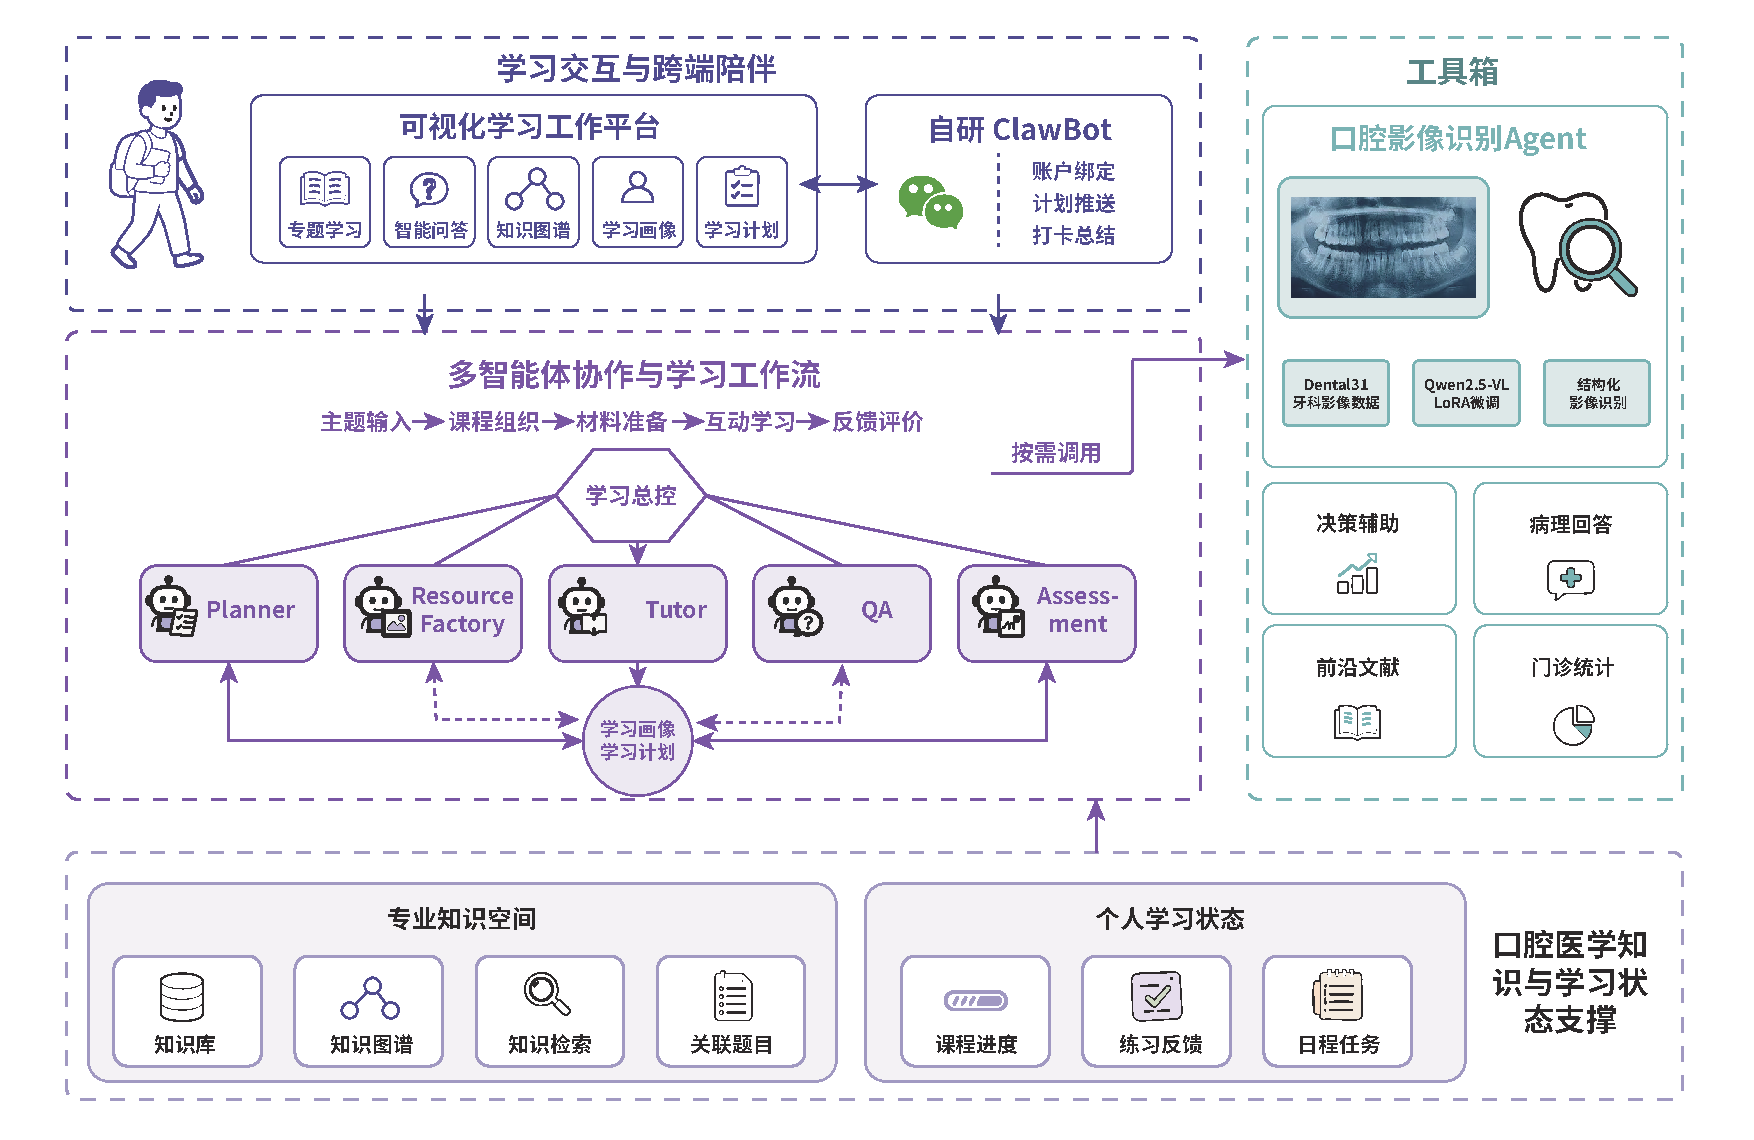
\includegraphics[width=\linewidth,height=8cm,keepaspectratio]{overall-architecture.pdf}
  \caption{OralSage 面向口腔医学个性化学习的总体架构}
  \label{fig:overall-architecture}
\end{figure}

从图\ref{fig:overall-architecture}可以看到，系统总体架构由四个相互连接的区域组成。上层是学习交互与跨端陪伴，承载专题学习、智能问答、知识图谱、学习画像、学习计划和 ClawBot 等学习入口；中层是多智能体协同与学习工作流，由学习总控协调 Planner、Resource Factory、Tutor、QA 和 Assessment 等 Agent；右侧是按需调用的专业工具箱，为影像学习、病理问答、病例分析、文献阅读、统计查询和病历文书等任务提供专项能力；下层是专业知识空间与个人学习状态，为课程规划、资源生成、教学互动和练习反馈提供知识内容、关系结构和学习记录支撑。

数字问诊通过独立的临床训练服务进入系统，患者 Agent 读取脱敏病例事实并保持多轮交流，判官 Agent 读取知识库检索证据并完成五个领域的表达评价。两类 Agent 通过诊断确认状态完成交接，问诊启动、诊断确认、分项评分和训练完成等事件写入共享学习画像。该入口与课程学习共同使用知识空间和个人学习状态，同时保留适合实时问诊的会话状态与接口边界，详细设计见第~\ref{sec:digital-consultation}章。

在知识与服务支撑层，系统将口腔医学知识库、知识图谱、专业资料片段和关联题目组织为统一的知识空间，并通过知识检索为课程规划、智能问答和练习反馈提供相关内容。当前知识底座覆盖 14 门口腔医学学科，包含 1,390 个核心条目、9,907 个知识概念、5,758 条知识关系和 3,161 道关联题目。

在此基础上，平台工具箱提供影像识别、决策辅助、门诊统计、前沿文献和病理问答等独立工具 Agent。其中，影像识别模块采用以 Qwen2.5-VL 为基座的牙科影像 LoRA 适配训练方案，为口腔影像学习和相关专业分析提供多模态能力。在跨端学习方面，自研 ClawBot 连接网页工作台与微信学习场景，支持账户绑定和学习计划推送，使学习者能够在日常沟通环境中接收任务提醒，并持续执行和跟进学习安排。

\section{专业学习闭环}

专业学习闭环描述学习者从提出主题到完成一次学习单元的过程。学习者输入学习主题后，系统结合专业知识内容和当前学习状态组织课程单元，并准备相应的讲义、课件、讲解和练习。进入课程后，学习者沿当前单元进行学习，可以在讲解过程中发起问题，也可以通过练习检验对知识内容的理解。

课程内的提问和作答反馈都会围绕当前主题和当前单元组织。QA Agent 负责补充解释，Assessment Agent 负责反馈正误、分析错因并提示需要回顾的内容。完成一个学习单元后，系统保留当前课程位置和学习结果，为继续学习或进入下一单元提供衔接。

\begin{center}
  \textbf{学习主题 $\rightarrow$ 课程与材料 $\rightarrow$ 分节学习与互动 $\rightarrow$ 练习反馈 $\rightarrow$ 学习状态 $\rightarrow$ 学习计划}
\end{center}

这一流程将主题输入、课程材料、分节学习、互动答疑和练习反馈组织为一次连续的课程会话，使学习者能够在保持课程主线的同时完成理解检验，并获得进入下一学习单元的明确衔接。

\section{学习状态驱动的持续陪伴}

OralSage 以学习画像汇集课程进度、练习反馈和学习偏好，并将这些学习状态转化为学习计划中的具体任务。学习画像通过学习活动趋势、阶段摘要和学习偏好等可视化信息呈现个人进展，学习者可以据此了解当前学习重点。完成课程或练习后，后续复习重点和日程安排随之更新，使学习记录能够自然进入下一阶段学习。

数字问诊进一步提供来自临床表达过程的细粒度信号。诊断是否正确、五个领域的分项得分和遗漏要点会更新知识节点掌握度与薄弱点，下一次病例选择再读取这些内容。学习者在课程中形成的知识状态可以影响病例训练，病例训练呈现出的表达缺口也能回到后续课程与复习安排，构成跨学习场景的动态联系。

学习计划以日历和待办承接课程内容与复习任务，学习者可以结合自己的时间安排完成、延期或调整任务。自研 ClawBot 连接网页工作台与微信学习场景，支持账户绑定和学习计划推送。学习者能够在日常沟通环境中接收任务提醒，并回到平台继续课程与计划执行，使学习陪伴覆盖更自然的使用场景。

% !TeX root = ../main.tex

\chapter{多智能体协同、Skill 封装与工具调用设计}
\label{sec:multi-agent}

\definecolor{chthreeaccent}{HTML}{E9E9F5}
\tikzset{
  cthreebox/.style={draw=black!70, rounded corners=2pt, fill=white, align=center, minimum height=0.92cm, text width=2.35cm, font=\small},
  cthreemain/.style={draw=black!78, rounded corners=2pt, fill=chthreeaccent, align=center, minimum height=1.02cm, text width=2.55cm, font=\small\bfseries},
  cthreedata/.style={draw=black!58, rounded corners=2pt, fill=black!5, align=center, minimum height=0.88cm, text width=2.5cm, font=\small},
  cthreewarn/.style={draw=black!70, rounded corners=2pt, fill=black!8, align=center, minimum height=0.88cm, text width=2.55cm, font=\small},
  cthreearrow/.style={->, >=stealth, thick, draw=black!78},
  agentinput/.style={draw=black!72, line width=.65pt, rounded corners=2pt, fill=white, align=center, minimum height=1.02cm, text width=2.25cm, font=\scriptsize},
  agentcore/.style={draw=black!78, line width=.8pt, rounded corners=2pt, fill=chthreeaccent, align=center, minimum height=1.08cm, text width=2.35cm, font=\scriptsize\bfseries},
  agentprocess/.style={draw=black!68, line width=.65pt, rounded corners=2pt, fill=black!3, align=center, minimum height=1.02cm, text width=2.2cm, font=\scriptsize},
  agentoutput/.style={draw=black!72, line width=.65pt, rounded corners=2pt, fill=white, align=center, minimum height=1.02cm, text width=2.3cm, font=\scriptsize},
  agentmemory/.style={draw=black!55, line width=.55pt, rounded corners=2pt, fill=black!5, align=center, minimum height=.72cm, text width=4.0cm, font=\scriptsize},
  agentarrow/.style={->, >=stealth, line width=.7pt, draw=black!78},
  agentfeedback/.style={->, >=stealth, line width=.65pt, dashed, draw=black!58}
}

\section{学习资源 Agent 设计与协作}

OralSage 围绕口腔医学主题学习展开路径规划、材料组织、连续讲解、即时答疑、理解检验和章节推进等相互衔接的教学活动。学习资源 Agent 群围绕同一学习会话协同工作，课程单元、讲义章节、知识图谱关系、学习进展和答题表现持续贯穿各个环节。学习者既能围绕当前需求启动某项专业能力，也能从一个主题进入具有完整结构的连续课程，系统会在不同学习时刻调动最契合的 Agent 参与教学。

这种设计让学习资源从静态内容扩展为动态生长的教学环境。课程规划提供知识理解的主线，讲义与多模态材料丰富学习媒介，讲解与答疑持续深化理解，测评与后续章节共同推动学习进展。对学习者而言，每一轮学习活动都能够回到当前主题、当前章节和当前学习状态，既保持课程结构的连续性，也保留按需探索的灵活性。

\begin{figure}[H]
  \centering
  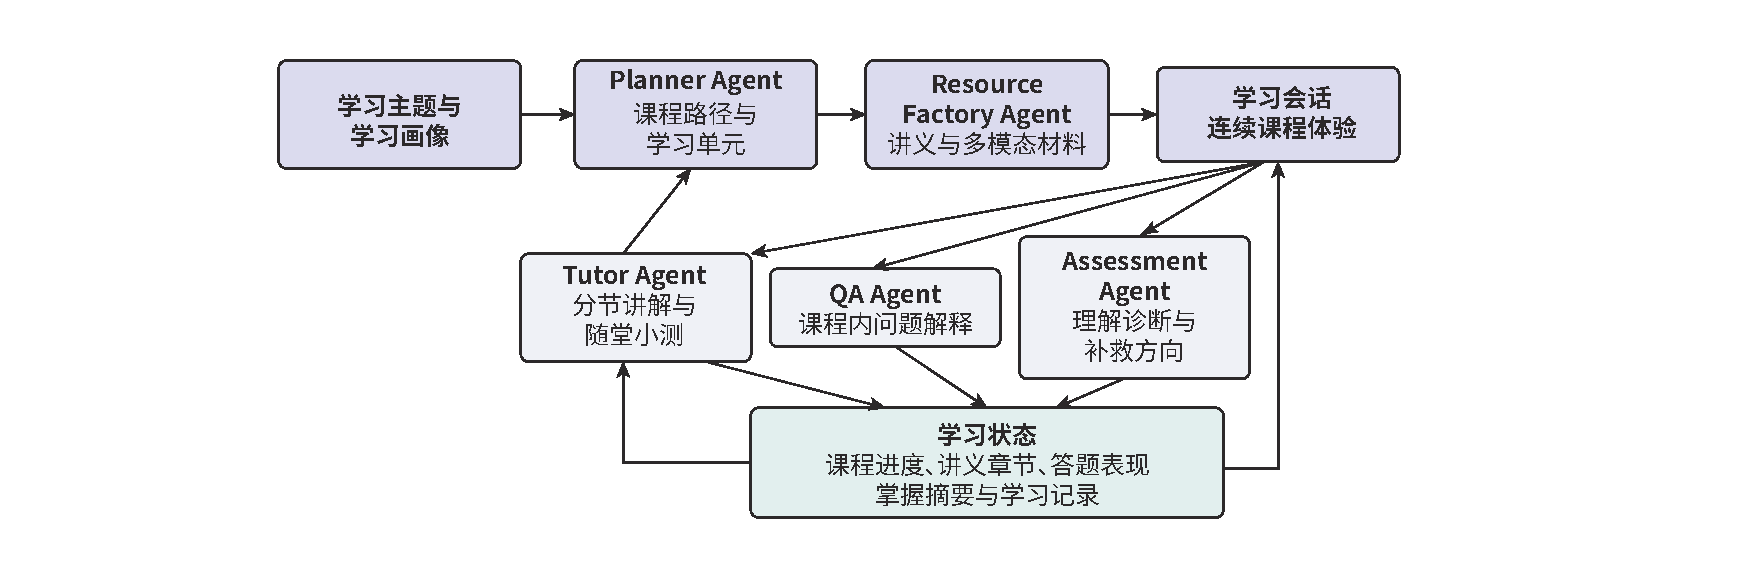
\includegraphics[width=0.96\linewidth]{Collaboration-between-learning-resources-and-agents.pdf}
  \caption{学习资源 Agent 群的协同关系}
  \label{fig:agent-overall-architecture}
\end{figure}

\subsection{Planner Agent}

主题进入课程后，Planner Agent 会综合学习主题、学习者画像、知识图谱节点、概念关系、资料片段和关联题目，编织由多个学习单元组成的课程路径。每个单元都围绕明确的理解目标展开，编排理由、知识范围和资料范围也会写入单元设计。口腔医学中病因机制、临床表现、诊断思路与治疗原则之间存在天然依赖，课程顺序能够沿着知识结构逐步展开，帮助学习者从概念建立走向重点理解。

Planner Agent 为整个学习资源体系确立共同教学语境，使 Resource Factory 能够围绕当前章节准备材料，Tutor 能够承接前后章节进行讲解，QA 能够理解问题所处的课程位置，Assessment 能够把作答表现映射到相关知识内容。对学习者而言，Planner Agent 的核心价值不只是排列课程单元，而是把分散的知识、资料和题目组织成一条可以执行的学习路径。学习者无需反复判断“先学什么、后学什么”，即可沿着清晰的主线逐步完成主题学习。

\begin{figure}[H]
  \centering
  \resizebox{\linewidth}{!}{%
  \begin{tikzpicture}[node distance=.5cm and .48cm]
    \node[font=\small\bfseries] at (6.85,1.25) {Planner Agent 工作流};
    \node[agentinput] (pinput) at (0,0) {主题学习请求\\学习画像与课程进展};
    \node[agentcore, right=of pinput] (pcontext) {主题语境聚合\\知识关系、资料与题目};
    \node[agentprocess, right=of pcontext] (pstructure) {知识结构编排\\前后概念依赖与重点};
    \node[agentcore, right=of pstructure] (punit) {学习单元设计\\目标、顺序与学习范围};
    \node[agentoutput, right=of punit] (ppath) {课程路径\\可进入的首个学习单元};
    \node[agentmemory, below=1.0cm of pstructure] (pmemory) {学习状态回流：章节进展、答题表现、掌握摘要与互动历史};
    \draw[agentarrow] (pinput) -- (pcontext);
    \draw[agentarrow] (pcontext) -- (pstructure);
    \draw[agentarrow] (pstructure) -- (punit);
    \draw[agentarrow] (punit) -- (ppath);
    \draw[agentfeedback] (ppath.south) |- (pmemory.east);
    \draw[agentfeedback] (pmemory.west) -| (pcontext.south);
  \end{tikzpicture}}
  \caption{Planner Agent 的课程路径规划工作流}
  \label{fig:planner-workflow}
\end{figure}

\subsection{Resource Factory Agent}

课程路径确定后，Resource Factory Agent 围绕学习单元组织讲义、课件、讲稿、语音、思维导图和练习材料。讲义生成遵循“资料规划、内容写作”的两阶段教学策略。前一阶段聚焦本节核心知识、资料组合和表达重点，后一阶段依据已经准备好的资料组织具有教学层次的讲义内容。课程目标、知识关系和重点概念持续贯穿材料生成过程，学习者能够在内容中感受到清晰的专业表达和稳定的章节主题。

同一学习单元还会延展出讲义、课件、文字讲解、语音讲解和思维导图等多种媒介形态。这些材料分别承担理论梳理、重点呈现、听觉讲解和复习辅助等作用，共同帮助学习者建立知识框架、理解重点内容，并完成后续练习与复习。学习者可以在阅读、浏览、听讲和练习之间自然切换，而不必重新寻找与当前主题对应的学习材料。首节优先的准备节奏进一步缩短主题学习的启动时间，随着课程推进，课程材料持续丰富，使课程体验兼具完整性和流畅性。

\begin{figure}[H]
  \centering
  \resizebox{\linewidth}{!}{%
  \begin{tikzpicture}[node distance=.5cm and .48cm]
    \node[font=\small\bfseries] at (6.85,1.25) {Resource Factory Agent 工作流};
    \node[agentinput] (rinput) at (0,0) {学习单元\\目标、范围与知识关系};
    \node[agentcore, right=of rinput] (rplan) {资料规划\\重点概念与材料组合};
    \node[agentprocess, right=of rplan] (rwrite) {教学内容组织\\层次、节奏与表达重点};
    \node[agentcore, right=of rwrite] (rmedia) {多媒介延展\\讲义、课件、讲稿、语音};
    \node[agentoutput, right=of rmedia] (rresult) {学习资源包\\围绕单元一致呈现};
    \node[agentmemory, below=1.0cm of rwrite] (rstate) {课程语境贯穿：当前章节、学习主题、概念脉络与后续活动};
    \draw[agentarrow] (rinput) -- (rplan);
    \draw[agentarrow] (rplan) -- (rwrite);
    \draw[agentarrow] (rwrite) -- (rmedia);
    \draw[agentarrow] (rmedia) -- (rresult);
    \draw[agentfeedback] (rresult.south) |- (rstate.east);
    \draw[agentfeedback] (rstate.west) -| (rplan.south);
  \end{tikzpicture}}
  \caption{Resource Factory Agent 的多媒介资源生成工作流}
  \label{fig:resource-factory-workflow}
\end{figure}

\subsection{Tutor Agent}

Tutor Agent 通过承接讲义内容、前后章节关系、学习位置、相关知识节点和掌握摘要，以更贴近教学语言的方式展开分节讲解，使得病因机制、临床表现、诊断思路和治疗原则之间的关联能够在连续表达中逐步展开，学习者既能理解当前概念，也能把握其与前后知识内容之间的联系。章节过渡、重点提示和即时小测共同让每一次讲解保持清晰的学习焦点。

学习者可以直接发起当前章节讲解，或根据自己的理解情况请求调整表达方式；Tutor 也会随着总控调度伴随课程进展持续出现。由于讲解始终承接当前章节、学习位置和已有掌握情况，学习者不需要每次重新说明背景，就可以继续上一次学习过程。每一轮讲解既承担知识解释，也承担学习节奏提示，使学习者能够持续感知已经理解的内容、正在学习的位置和下一步方向，形成接近一对一辅导的连续体验。

\begin{figure}[H]
  \centering
  \resizebox{\linewidth}{!}{%
  \begin{tikzpicture}[node distance=.5cm and .48cm]
    \node[font=\small\bfseries] at (6.85,1.25) {Tutor Agent 工作流};
    \node[agentinput] (tinput) at (0,0) {当前学习单元\\讲义内容与学习位置};
    \node[agentcore, right=of tinput] (tprepare) {教学语境组织\\概念关系与掌握摘要};
    \node[agentprocess, right=of tprepare] (texplain) {分节讲解推进\\机制、表现、思路与原则};
    \node[agentcore, right=of texplain] (tinteract) {互动教学调节\\重点提示、过渡与即时小测};
    \node[agentoutput, right=of tinteract] (tresult) {连续讲解体验\\理解当前位置与下一步方向};
    \node[agentmemory, below=1.0cm of texplain] (tstate) {学习信号回流：讲解进度、互动偏好、理解摘要与章节状态};
    \draw[agentarrow] (tinput) -- (tprepare);
    \draw[agentarrow] (tprepare) -- (texplain);
    \draw[agentarrow] (texplain) -- (tinteract);
    \draw[agentarrow] (tinteract) -- (tresult);
    \draw[agentfeedback] (tresult.south) |- (tstate.east);
    \draw[agentfeedback] (tstate.west) -| (tprepare.south);
  \end{tikzpicture}}
  \caption{Tutor Agent 的连续讲解工作流}
  \label{fig:tutor-workflow}
\end{figure}

\subsection{QA Agent}

用户进行提问之后，系统调用 QA Agent，将当前问题与正在学习的单元、讲义内容、知识图谱关系、相关资料和近期对话联系在一起。围绕病因机制、概念辨析、检查思路或治疗原则等问题，QA 会先判断提问与当前章节之间的联系，再结合课程资料和主题检索展开解释。这样，学习者得到的不是脱离课程上下文的孤立答案，而是能够回到当前知识结构中的针对性说明，在解决眼前困惑的同时继续推进对主题的理解。


\begin{figure}[H]
  \centering
  \resizebox{\linewidth}{!}{%
  \begin{tikzpicture}[node distance=.5cm and .48cm]
    \node[font=\small\bfseries] at (6.85,1.25) {QA Agent 工作流};
    \node[agentinput] (qinput) at (0,0) {课程内追问\\当前单元与近期对话};
    \node[agentcore, right=of qinput] (qidentify) {问题语境辨析\\问题与章节位置关联};
    \node[agentprocess, right=of qidentify] (qretrieve) {主题资料联结\\讲义、知识关系与相关资料};
    \node[agentcore, right=of qretrieve] (qanswer) {深入解释组织\\概念辨析与机制阐释};
    \node[agentoutput, right=of qanswer] (qreturn) {回归课程主线\\带着理解继续学习};
    \node[agentmemory, below=1.0cm of qretrieve] (qstate) {课程语境保持：正在学习的章节、问题脉络与知识范围};
    \draw[agentarrow] (qinput) -- (qidentify);
    \draw[agentarrow] (qidentify) -- (qretrieve);
    \draw[agentarrow] (qretrieve) -- (qanswer);
    \draw[agentarrow] (qanswer) -- (qreturn);
    \draw[agentfeedback] (qreturn.south) |- (qstate.east);
    \draw[agentfeedback] (qstate.west) -| (qidentify.south);
  \end{tikzpicture}}
  \caption{QA Agent 的课程内即时解释工作流}
  \label{fig:qa-workflow}
\end{figure}

\subsection{Assessment Agent}

提交作答后，Assessment Agent 先核对选项与答案，再结合题目考查内容解释关键判断依据。出现偏差时，系统会定位容易混淆的概念，并把相关知识点和复习方向带回当前学习单元；答对时，则以简短提示强化本题的判断线索。练习结果能够转化为下一步学习的具体着力点。

Assessment Agent 能够将学习者的答题表现、相关知识点和知识点巩固方向写进学习状态中，使后续 Tutor 讲解、QA 追问和课程路径调节获得更具针对性的学习信号。对学习者而言，练习结果不再只是一次性的对错反馈，而会进一步转化为“哪些概念已经掌握、哪些地方容易混淆、下一步应该复习什么”的学习提示，成为知识掌握、学习反馈和后续学习之间的重要连接点。

\begin{figure}[H]
  \centering
  \resizebox{\linewidth}{!}{%
  \begin{tikzpicture}[node distance=.5cm and .48cm]
    \node[font=\small\bfseries] at (6.85,1.25) {Assessment Agent 工作流};
    \node[agentinput] (ainput) at (0,0) {练习作答\\当前主题与题目语境};
    \node[agentcore, right=of ainput] (ajudge) {作答理解\\选项识别与正误判断};
    \node[agentprocess, right=of ajudge] (aanalyze) {理解诊断\\误区、知识缺口与关联概念};
    \node[agentcore, right=of aanalyze] (adirect) {学习建议组织\\解析、复习重点与补救方向};
    \node[agentoutput, right=of adirect] (aresult) {学习推进信号\\服务后续讲解与课程调节};
    \node[agentmemory, below=1.0cm of aanalyze] (astate) {掌握状态更新：作答表现、薄弱知识点、复习方向与课程进展};
    \draw[agentarrow] (ainput) -- (ajudge);
    \draw[agentarrow] (ajudge) -- (aanalyze);
    \draw[agentarrow] (aanalyze) -- (adirect);
    \draw[agentarrow] (adirect) -- (aresult);
    \draw[agentfeedback] (aresult.south) |- (astate.east);
    \draw[agentfeedback] (astate.west) -| (ajudge.south);
  \end{tikzpicture}}
  \caption{Assessment Agent 的理解诊断与学习推进工作流}
  \label{fig:assessment-workflow}
\end{figure}

\subsection{叶子 Agent 群设计}

为了更好地协调学习系统的各类能力，OralSage 设计了叶子 Agent 群。这里的“叶子 Agent”是指能够直接完成某一项具体学习服务、也能够被上层课程流程组合调用的基础能力单元。它们把学习资源交付和学习推进拆解为一组可独立调用的专业能力。学习者可以根据当下需求快速获得讲义、课件、演示文稿、讲稿、语音、练习或继续学习体验；进入系统化主题课程后，这些能力又会围绕同一学习单元依次出现，形成材料准备、知识讲授、主动检验和章节推进之间的连续协作。

\paragraph{（1）讲义 Agent}
讲义 Agent 围绕课程单元组织结构化学习文本，重点概念、关键解释和章节脉络在此汇聚为便于阅读与复习的学习材料。课程知识由此以稳定、清晰的文本形态呈现，为后续讲解、答疑、课件和练习提供共同的学习基础。

\paragraph{（2）课件与演示文稿 Agent}
课件与演示文稿 Agent 把章节重点转化为视觉化学习材料。知识层次、关键概念和章节结构通过页面组织得到突出，学习者在快速浏览、课堂展示和阶段复习时能够更高效地把握内容主线，并与讲义、讲稿保持一致的学习节奏。

\paragraph{（3）教学讲稿与语音 Agent}
教学讲稿与语音 Agent 延展了阅读之外的连续学习场景。讲义内容经过教学化组织后形成自然的讲解节奏，语音学习进一步支持通勤、碎片时间和重复回顾等多种学习场景。学习者能够在不同时间和媒介中围绕同一主题持续学习。

\paragraph{（4）练习 Agent}
练习 Agent 围绕当前课程主题组织题目和阶段练习，把知识理解转化为主动检验。题目活动与课程单元同步，学习者能够在完成讲解后及时检查理解程度，并把作答表现带入后续的测评分析和学习推进。

\paragraph{（5）继续学习 Agent}
继续学习 Agent 承接当前学习单元的完成状态，组织进入下一章节的自然过渡。课程主线、当前进展和已经形成的学习记录会随着章节推进持续延续，学习者能够始终保持对整体路径和当前阶段的清晰感知。

\begin{figure}[H]
  \centering
  \resizebox{\linewidth}{!}{%
  \begin{tikzpicture}[node distance=.35cm and .45cm]
    \node[font=\small\bfseries] at (7.0,4.05) {叶子 Agent 群的按需调用与课程接续工作流};
    \node[agentinput, text width=2.1cm] (lin) at (0,0) {学习者当前需求\\或课程单元事件};
    \node[agentcore, text width=2.25cm] (ldoc) at (3.0,2.4) {讲义 Agent\\结构化学习文本};
    \node[agentcore, text width=2.25cm] (lslide) at (3.0,1.2) {课件与演示文稿 Agent\\重点视觉化呈现};
    \node[agentcore, text width=2.25cm] (laudio) at (3.0,0) {教学讲稿与语音 Agent\\连续讲解媒介};
    \node[agentcore, text width=2.25cm] (lpractice) at (3.0,-1.2) {练习 Agent\\阶段性主动检验};
    \node[agentcore, text width=2.25cm] (lnext) at (3.0,-2.4) {继续学习 Agent\\单元衔接与推进};
    \node[agentprocess, text width=2.55cm] (lcontext) at (6.15,0) {共享学习语境\\主题、单元、章节进展\\知识关系与学习记录};
    \node[agentoutput, text width=2.45cm] (lout) at (9.3,0) {多样学习活动\\材料交付、讲解、练习\\与下一章节进入};
    \node[agentmemory, text width=2.5cm] (lstate) at (12.15,0) {学习状态\\课程轨迹持续更新};
    \draw[agentarrow] (lin.east) -| (ldoc.west);
    \draw[agentarrow] (lin.east) -| (lslide.west);
    \draw[agentarrow] (lin.east) -- (laudio.west);
    \draw[agentarrow] (lin.east) -| (lpractice.west);
    \draw[agentarrow] (lin.east) -| (lnext.west);
    \draw[agentarrow] (ldoc.east) -| (lcontext.west);
    \draw[agentarrow] (lslide.east) -| (lcontext.west);
    \draw[agentarrow] (laudio.east) -- (lcontext.west);
    \draw[agentarrow] (lpractice.east) -| (lcontext.west);
    \draw[agentarrow] (lnext.east) -| (lcontext.west);
    \draw[agentarrow] (lcontext) -- (lout);
    \draw[agentarrow] (lout) -- (lstate);
  \end{tikzpicture}}
  \caption{叶子 Agent 群围绕共享学习语境形成的并行服务流程}
  \label{fig:leaf-agent-workflow}
\end{figure}

\begin{table}[H]
  \centering
  \caption{学习资源 Agent 的职责边界与用户价值}
  \label{tab:agent-boundaries}
  \begin{tabularx}{\linewidth}{p{0.22\linewidth}p{0.35\linewidth}X}
    \toprule
    Agent 类型 & 课程学习中的能力表现 & 学习体验提升 \\
    \midrule
    Planner Agent & 组织知识结构、学习顺序与单元目标 & 课程主线清晰，学习路径由浅入深 \\
    Resource Factory Agent & 形成讲义与多模态学习材料 & 多种学习媒介围绕同一知识主题协同展开 \\
    Tutor 与 QA Agent & 提供连续讲解和课程内深入解释 & 讲解、追问和继续学习保持自然衔接 \\
    Assessment Agent & 展开作答分析、误区解释与补救方向 & 练习结果能够进入后续学习调节 \\
    叶子 Agent 群 & 支持讲义、课件、讲稿、语音、练习和章节推进 & 学习者能够按需组合多样化学习活动 \\
    \bottomrule
  \end{tabularx}
\end{table}

\section{工具 Agent}

除课程学习能力外，OralSage 在影像、病理、病例、文献、知识图谱、统计和病历文书等专业能力上也设计了工具 Agent，服务于更深层的口腔医学学习，并为课程中的案例讨论、资料查阅和知识延展带来丰富的专业信息。影像分析、病理问答、决策辅助和文献阅读体现了工具 Agent 最具代表性的专业价值。

影像分析 Agent 涉及口腔影像数据治理、OralPath 视觉模型微调、本地推理部署和结构化多模态输出，已经从本章工具 Agent 总览中拆分为独立章节，详见第~\ref{sec:image-analysis-agent}章。本节后续重点说明其他专业工具 Agent 的协作职责。

\subsection{病理问答 Agent}

病理问答 Agent 面向口腔病理专题学习，本地专业资料、主题检索和前沿文献线索会汇聚到同一问题语境中。学习者围绕疾病机制、典型表现、诊断思路、鉴别要点和处理原则展开研读时，系统会组织结构化的病理学习内容，并呈现相应的资料依据和研究线索。抽象的病理概念能够与临床表现和学习问题建立更紧密的联系。

这一 Agent 特别适合服务于专题复习、课程案例讨论和病理机制深化学习。学习者能够从一个具体问题进入多层次的专业解释，再回到当前课程主题继续学习，病理知识由此成为连接基础理论和口腔医学应用的重要桥梁。

\subsection{决策辅助 Agent}

决策辅助 Agent 面向脱敏病例文本组织口腔医学案例研读。主诉、现病史、口内检查、影像资料和风险信息共同进入病例理解过程，系统围绕诊断依据、鉴别方向、检查建议、处理原则和风险关注点形成清晰的分析脉络。复杂病例信息以适合学习讨论的结构呈现，学习者能够沿着临床思维路径理解信息之间的关联。

病例分析过程还会结合口腔医学知识库和专题资料组织重点内容，使案例学习兼具专业知识深度和情境理解价值。对于医学生和口腔医学学习者而言，这一 Agent 能够把教材中的知识点带入更接近真实专业讨论的场景，强化从知识理解到案例思考的迁移能力。

\subsection{文献阅读 Agent}

文献阅读 Agent 围绕口腔医学主题开展术语理解、检索词组织、PubMed 与 Elsevier 文献检索、研究资料整理和中文阅读支持。学习者提出前沿问题后，系统能够把专业主题转化为更贴近学术检索的关键词，并整合不同来源的研究资料，帮助学习者快速进入某一方向的研究脉络。

检索结果以题名、来源、摘要、链接和综合解读等形式组织，英文研究内容可以进一步进入中文阅读流程。课程知识与前沿研究由此获得自然连接，学习者能够在专题学习过程中同步理解教材中的稳定知识和最新研究中的发展方向。

知识浏览、知识图谱、临床统计和病历文书工具进一步扩展了专业工具箱的能力广度。教材知识点、概念关联和局部知识网络支持专题探索，结构化门诊数据支持统计学习与图表分析，语音转写修订、信息提取和文书生成则带来面向口腔医学文书场景的综合学习体验。

\section{总控调度器设计}

总控调度器让自主学习请求和系统化主题课程进入同一协作体系。学习者可以直接提出“生成讲义”“准备课件”“讲解当前章节”“出一组练习题”等明确需求，相关 Agent 会快速进入当前学习活动。学习者也可以从“系统学习某一主题”开启完整课程，总控随后结合主题、学习画像、课程单元、讲义进展、互动历史和掌握摘要组织多 Agent 协作。两种入口共享同一学习会话，使自由探索与连续课程在体验上保持一致。

课程推进过程中，总控调度器持续理解学习者的行为变化。继续学习意味着当前章节需要更深入的讲解，课程内追问会带来 QA 的解释活动，提交作答会引导 Assessment 展开理解诊断，章节完成后则进入下一单元的材料与讲解准备。学习者的每次交互都丰富了会话语境，总控据此选择合适的 Agent 和学习动作，让多个专业角色在恰当时机自然接续。

\begin{figure}[H]
  \centering
  \begin{tikzpicture}[>=stealth]
    \node[agentinput] (input) at (0,0) {学习者互动\\继续、提问、作答或学习偏好};
    \node[agentinput] (state) at (3.5,0) {学习会话\\当前单元、进度与学习记录};
    \node[agentcore] (policy) at (7.0,0) {总控调度器\\识别下一步学习动作};
    \node[agentprocess] (check) at (7.0,-1.9) {课程调度检查\\学习情境、角色与课程进展};
    \node[agentoutput] (tutor) at (3.5,-3.8) {Tutor\\连续讲解};
    \node[agentoutput] (qa) at (7.0,-3.8) {QA\\即时解释};
    \node[agentoutput] (assessment) at (10.5,-3.8) {Assessment\\理解诊断};
    \node[agentmemory, text width=5.8cm] (result) at (7.0,-5.45) {学习进展与状态更新};
    \draw[agentarrow] (input) -- (state);
    \draw[agentarrow] (state) -- (policy);
    \draw[agentarrow] (policy) -- (check);
    \draw[agentarrow] (check.south west) -- (tutor.north);
    \draw[agentarrow] (check) -- (qa);
    \draw[agentarrow] (check.south east) -- (assessment.north);
    \draw[agentarrow] (tutor.south) -- (result.north west);
    \draw[agentarrow] (qa.south) -- (result.north);
    \draw[agentarrow] (assessment.south) -- (result.north east);
    \draw[agentfeedback] (result.west) to[out=160,in=-90] (state.south);
  \end{tikzpicture}
  \caption{总控调度器驱动的会话内 Agent 协同}
  \label{fig:session-policy-routing}
\end{figure}

\section{工作流编排}

\subsection{主题学习主工作流}

主题学习工作流从知识上下文汇聚开始。相关知识图谱节点、概念关系、资料片段和题目共同描绘主题的知识范围，Planner Agent 据此建立学习单元与课程顺序。首节单元随后进入讲义和多模态材料准备，学习者进入会话后获得 Tutor 的连续讲解，并在需要时接入 QA 的即时解释和 Assessment 的理解检验。课程进展、互动行为和练习表现持续进入学习状态，下一轮教学活动由此能够建立在已经形成的学习经历之上。

工作流的灵活性体现在学习活动能够根据用户需求和会话进展动态组合。学习者可以从某一单项能力直接开始，也可以从完整课程进入后在任何章节发起讲解、提问、练习或材料生成。总控调度器把这些分散动作重新组织为面向当前课程目标的连续体验，课程主线始终清晰，学习过程也具备充分的探索空间。

\begin{algorithm}[H]
  \caption{主题学习的动态工作流编排}
  \label{alg:dynamic-dispatch}
  \begin{algorithmic}[1]
    \Require 学习主题、学习画像、知识上下文与学习者互动
    \Ensure 连续学习会话、多 Agent 协同结果与学习状态
    \State 汇聚主题相关知识结构、资料片段和关联题目
    \State 规划课程单元与学习顺序，准备首个学习单元
    \State 组织讲义、课件、讲稿、语音和练习等学习材料
    \State 启动学习会话，围绕当前单元开展连续讲解
    \While{课程处于学习状态}
      \State 理解学习者的继续学习、课程提问、练习作答和学习偏好
      \State 调度最契合当前学习情境的 Agent 进入本轮教学活动
      \State 汇入讲解、答疑和测评产生的学习信号
      \State 根据课程进展组织下一章节或下一轮学习活动
    \EndWhile
    \Return 具有课程轨迹和学习记录的主题学习体验
  \end{algorithmic}
\end{algorithm}

\subsection{多阶段内容生成}

内容生成围绕课程单元逐步展开。资料规划阶段明确本节知识重点和材料组合，讲义写作阶段形成具有教学层次的文本内容，课件、演示文稿、讲稿、语音、导图和练习随后围绕同一单元延展。多种材料共享章节主题和概念顺序，学习者在不同媒介之间切换时能够保持稳定的理解脉络。

首节优先的课程准备节奏让学习者更早进入主题学习，后续材料随着学习进展持续丰富。课程资源、连续讲解和即时互动由此形成相互呼应的学习环境，主题学习兼具整体路径与细节探索的灵活性。

\section{Skill 设计}

在上述工作流基础上，完整主题学习被进一步抽象为可复用的知识点学习 Skill。工作流描述的是一次主题学习运行时如何推进，Skill 则把这套推进方式封装为可以被系统调用的教学剧本。课程规划、讲义准备、课件生成、教学讲解、讲稿、语音、答疑、练习和学习状态更新沿着明确时序进入同一会话。学习者提出系统学习需求后，Skill 带动多 Agent 进入课程协作；在需要时，系统也可以调用其中的单项能力，为学习者提供更灵活的学习入口。

Skill 还让独立能力与完整课程保持自然衔接。学习者既可以直接请求某项学习服务，也可以在系统化课程中调用相同能力继续深化当前章节。课程规划、材料准备、教学互动和学习状态共同保持一致，学习者在自由探索和连续学习之间获得顺畅的体验转换。

\begin{figure}[H]
  \centering
  \begin{tikzpicture}[>=stealth]
    \node[agentinput] (input) at (0,0) {学习请求\\主题、画像与学习范围};
    \node[agentcore] (skill) at (3.6,0) {知识点学习 Skill\\完整课程任务编排};
    \node[agentoutput] (result) at (7.2,0) {学习会话\\连续课程体验与阶段轨迹};
    \node[agentprocess] (plan) at (0,-2.15) {课程规划\\学习单元与顺序};
    \node[agentprocess] (material) at (3.6,-2.15) {材料准备\\讲义、课件与练习};
    \node[agentprocess] (teach) at (7.2,-2.15) {教学互动\\讲解、答疑与测评};
    \node[agentmemory] (write) at (10.8,-2.15) {学习状态更新\\学习事件与画像信号};
    \draw[agentarrow] (input) -- (skill);
    \draw[agentarrow] (skill) -- (result);
    \draw[agentarrow] (skill.south) -- (material.north);
    \draw[agentarrow] (plan) -- (material);
    \draw[agentarrow] (material) -- (teach);
    \draw[agentarrow] (teach) -- (write);
    \draw[agentfeedback] (write.north) to[out=75,in=-35] (result.south);
  \end{tikzpicture}
  \caption{知识点学习 Skill 的课程编排逻辑}
  \label{fig:learning-skill-composition}
\end{figure}

\begin{lstlisting}[caption={知识点学习 Skill 编排示意},label={lst:learning-skill}]
skill "知识点学习" {
  课程路径 <- 规划主题学习路径(主题, 画像, 知识上下文)
  学习材料 <- 准备首个学习单元(课程路径)
  学习会话 <- 启动连续学习(课程路径, 学习材料)

  while 学习会话处于进行中:
      讲解当前单元
      响应课程内追问
      解析练习表现
      组织下一轮学习活动
}
\end{lstlisting}

\section{MCP 工具与专业知识增强}

MCP 工具层把专业检索和术语理解引入多 Agent 学习体系。口腔医学知识库检索、口腔医学术语解析、PubMed 检索和 Elsevier 检索共同扩展课程学习和专题探索的信息广度。课程规划能够从主题资料中组织学习内容，QA 能够围绕当前问题深化解释，病理问答和文献阅读 Agent 也能进入更丰富的专业资料语境。

知识库检索连接教材知识与当前学习主题，术语解析帮助学习者理解专业表达，PubMed 与 Elsevier 则为前沿研究学习提供权威资料入口。检索结果以结构化内容进入后续学习活动，课程知识、专题讨论和研究阅读因而能够形成更紧密的联系。检索增强医疗人工智能研究表明，专业资料与生成式系统协同能够增强复杂健康教育任务的信息支撑\cite{collaco2026ft_rag}。OralSage 通过专业工具、学习会话和多智能体协作，把这一能力转化为口腔医学学习中的持续价值。

\begin{figure}[H]
  \centering
  \resizebox{\linewidth}{!}{%
  \begin{tikzpicture}[>=stealth]
    \node[agentinput] (agents) at (0,0) {学习与工具 Agent\\规划、答疑、病理与文献服务};
    \node[agentcore] (mcp) at (3.5,0) {MCP 工具层\\主题检索与结构化资料};
    \node[agentprocess] (kb) at (6.9,1.35) {知识库检索\\主题资料与相关性说明};
    \node[agentprocess] (term) at (10.2,1.35) {术语解析\\口腔医学概念理解};
    \node[agentprocess] (pubmed) at (6.9,-1.35) {PubMed 检索\\口腔医学前沿文献};
    \node[agentprocess] (elsevier) at (10.2,-1.35) {Elsevier 检索\\口腔医学研究资料};
    \node[agentmemory, text width=2.9cm] (return) at (13.5,0) {结构化资料返回\\查询主题、资料数量与内容摘要};
    \draw[agentarrow] (agents) -- (mcp);
    \draw[agentarrow] (mcp.east) -- (kb.west);
    \draw[agentarrow] (mcp.east) -- (pubmed.west);
    \draw[agentarrow] (kb) -- (term);
    \draw[agentarrow] (pubmed) -- (elsevier);
    \draw[agentarrow] (term.east) -- (return.north west);
    \draw[agentarrow] (elsevier.east) -- (return.south west);
    \draw[agentfeedback] (return.south) to[out=-130,in=-30] (agents.south);
  \end{tikzpicture}}
  \caption{MCP 工具层对口腔医学学习与专题探索的支持}
  \label{fig:mcp-tool-layer}
\end{figure}

% !TeX root = ../main.tex

\chapter{影像分析 Agent：模型微调与推理}
\label{sec:image-analysis-agent}

本项目在模型层面的设计目标，并不是简单完成牙科影像的目标检测，而是在通用视觉语言模型的基础上，构建一个能够适配口腔场景的多模态专用模型，使其既能识别牙科影像中的关键目标，又能够以中文完成结构化描述、结果摘要和后续问答推理。基于这一目标，项目整体采用“通用多模态基座+领域指令数据+分阶段 LoRA 微调+本地推理部署”的技术路线。影像分析 Agent 正是该技术路线在 OralSage 系统中的工程封装：前端负责影像上传与结果展示，后端负责多模态请求构造与模型服务调用，OralPath-VL 视觉模型负责完成口腔影像理解与结构化输出。

\section{微调数据集}

本项目在模型适配部分主要使用团队自行整理的专门针对牙科疾病诊断设计的高精度多模态数据集。该数据集涵盖了 31 类口腔病理特征、治疗状态及解剖结构。

该数据集共包含 31 类牙科结构与病变目标，覆盖 4 大口腔临床领域，如表~\ref{tab:oralpath-target-overview} 所示。

\begin{table}[H]
  \centering
  \caption{牙科结构与病变目标概述}
  \label{tab:oralpath-target-overview}
  \small
  \renewcommand{\arraystretch}{1.18}
  \begin{tabularx}{\linewidth}{p{0.20\linewidth}X}
    \toprule
    领域 & 类别 \\
    \midrule
    牙体牙髓 & Caries（龋坏）、Filling（充填）、Root Canal Treatment、Periapical lesion、Root resorption、Fracture teeth \\
    修复/种植 & Crown（牙冠）、Implant（种植体）、Abutment、Post-core、Retained root、Root Piece \\
    牙周/颌骨 & Bone Loss、Bone defect、Cyst（囊肿）、Maxillary sinus、Mandibular Canal \\
    正畸/其他 & Orthodontic brackets、Wire、Metal band、TAD、Permanent retainer、Malaligned、Missing teeth、Supra Eruption 等 \\
    \bottomrule
  \end{tabularx}
\end{table}

经过前述处理方案后，本项目团队获得了三类基础任务数据：

1、结构化定位任务，用于训练模型识别图中目标并输出标准化的 JSON 结果；

2、中文摘要任务，用于训练模型根据牙科影像中的已标注信息生成较符合临床表达习惯的中文摘要；

3、长尾类别聚焦任务，用于针对低频类别进行专项补强。最终，这些数据又被统一整合为混合型训练数据集，用于后续多任务联合训练。

\begin{figure}[H]
  \centering
  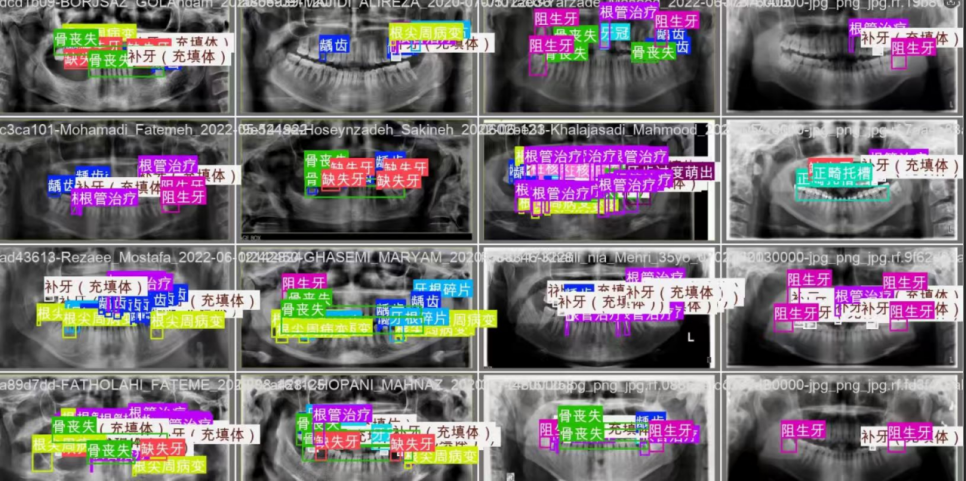
\includegraphics[width=0.96\linewidth]{oralpath-fig17-multimodal-data.png}
  \caption{高精度多模态数据部分示意}
  \label{fig:oralpath-multimodal-data}
\end{figure}

根据上述数据集的特性与 OralSage 项目的定位，本项目设计了如下模型微调方案，使模型在保持通用能力的同时具备更强的口腔专业理解能力。

\section{基座模型}

本项目采用“通用大模型推理 + 专科小模型微调”的组合架构。

在 Agent 实际运行中，调用 Pro/Qwen/Qwen2.5-7B-Instruct 处理纯文本逻辑，调用 volcano 处理语音交互，从而保证日常对话、文本理解和语音输入输出具有较好的稳定性与响应速度；而在口腔影像识别、多模态理解和图文联合推理等核心任务上，项目团队并未直接依赖通用模型，而是单独选择一套适合作为领域微调基座的视觉语言模型，用于构建面向口腔场景的专用多模态能力。

结合项目的实际需求与运行环境，本项目最终选取 Qwen/Qwen2.5-VL-7B-Instruct 作为微调基座模型。其选择并非单纯因为参数规模适中，而是综合考虑了口腔影像的图像特点、多模态任务形式、以及后续本地部署的可行性。从整体原则上看，本项目的模型选型主要围绕四个关键词展开：适配口腔影像特点、支持多模态推理、能够稳定调用，以及具备较好的轻量化与工程部署能力。

1、视觉感知适配性：面向口腔特殊影像结构

口腔全景片（OPG）具有“幅面宽、细节密”的特点。若使用常规 VLM，往往需要对图像进行填充（Padding）或拉伸，导致无效计算或特征变形。本项目利用 Qwen2.5-VL 的 M-RoPE（旋转位置编码）机制，将全景片切分为多个 Patch 进行序列化输入，在不增加显存开销的前提下，实现了对全景片原始分辨率的完整保留。

2、多模态推理一致性：支持图文联合决策场景

口腔诊疗决策是典型的多模态任务（X 光 + 主诉 + 既往史）。Qwen2.5-VL 支持图像与长文本的交错输入（Interleaved Input），使得系统可以将“患者全景片”与“RAG 召回的文本指南”作为一个完整的 Prompt 输入给模型。这种设计避免了传统“视觉模型看图 + 语言模型看文”的分离式架构带来的语义损耗，显著提升了解释型回答（Explainable AI）的准确性。

3、模型规模与成本平衡：兼顾效果与训练部署效率

对于口腔领域这样的垂直场景，项目目标不是训练一个超大规模通用模型，而是在有限的时间和算力约束下，构建一个“足够强、且可部署”的专科视觉语言模型。如果选择更大规模的多模态模型，虽然可能在通用任务上有更强的上限，但训练成本、显存占用、推理时延以及后续部署复杂度都会明显提升，不利于项目在竞赛场景与实际平台中的快速落地。而 7B 级别模型在当前硬件环境下已经能够较好地支撑 LoRA 微调、本地测试和后续服务封装，同时在效果与效率之间取得较合理平衡。

4、工程接入可行性：适配本地服务链路

Qwen2.5-VL 作为当前社区中兼容性较好、生态较成熟的视觉语言模型，在本地推理服务构建、LoRA 微调适配、模型权重导出以及 OpenAI-compatible 接口封装方面都具有较好的工程基础，这使得项目团队可以在较短时间内打通“模型训练—模型评测—模型部署—平台接入”的闭环，而不必将大量精力消耗在底层兼容问题上。

\begin{figure}[H]
  \centering
  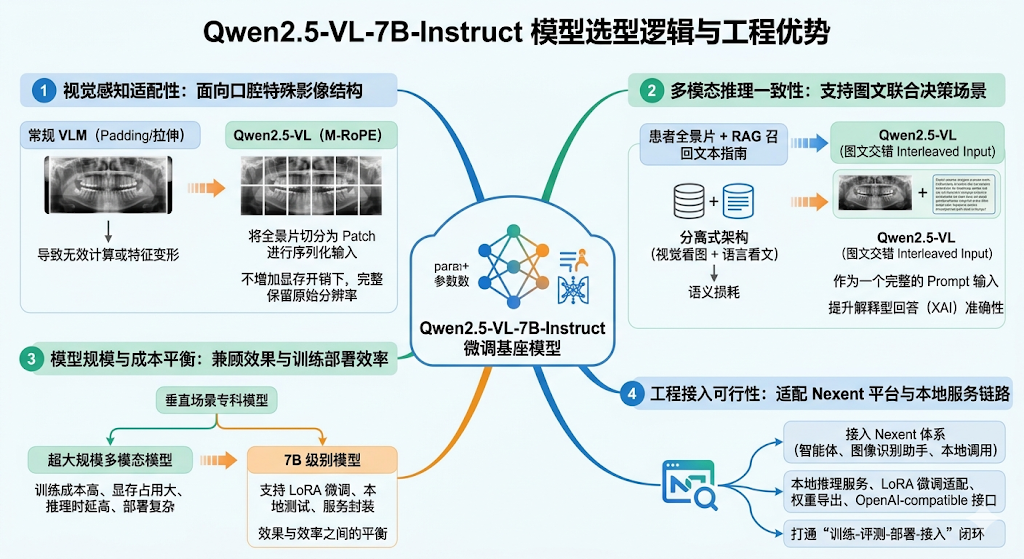
\includegraphics[width=0.96\linewidth]{oralpath-fig18-qwen-vl-design.png}
  \caption{Qwen2-VL-7B 模型微调设计思路}
  \label{fig:oralpath-qwen-vl-design}
\end{figure}

基于上述特性，项目团队采用 Qwen/Qwen2.5-VL-7B-Instruct 的微调版本作为“口腔多模态能力”的核心支撑模型。在此基础上，再利用口腔领域图像数据和转换后的多模态指令数据进行 LoRA 微调，使模型逐步获得面向牙科影像的目标识别、结构化定位、中文摘要表达和长尾类别补强能力。

从实际项目需求来看，本研究并不打算重新训练一个全新的牙科多模态模型，而是希望在高质量通用模型基础上，利用专科领域数据进行适配，使模型逐步获得口腔影像理解能力。采用 Qwen2.5-VL-7B-Instruct 作为基座，可以保留通用视觉语言推理能力，并通过较低成本的领域微调，使其更适合口腔场景中的图像理解与问答需求。

\section{设计思路概述}

模型微调的整体思路可以概括为“先建立主体能力，再补强薄弱类别，最后衔接推理和评测”。在训练逻辑上，项目并未采用单轮单任务微调方式，而是根据口腔场景的实际需求，将训练过程设计为分阶段的领域适配过程。

1、第一阶段：主训练阶段

该阶段使用混合型多任务数据集，让模型同时学习目标识别、位置表达和中文摘要能力。这样做的目的，是让模型优先建立对口腔影像中“主要对象”和“主要表达方式”的整体理解，而不是只停留在单一检测任务上。

2、第二阶段：长尾类别补强阶段

由于原始牙科数据中不同类别之间分布极不均衡，部分重要病变和器械类别样本数量很少，如果不单独强化，模型容易在高频类别上表现良好，却对稀有类别缺乏敏感性。因此，在主训练完成后，项目再使用长尾类别聚焦数据集对模型进行二次补强。

3、第三阶段：推理评测阶段

在微调完成后，通过快速评测和全量评测两种方式，对模型在测试集上的表现进行验证，并为后续本地部署和智能体调用提供依据。

\begin{figure}[H]
  \centering
  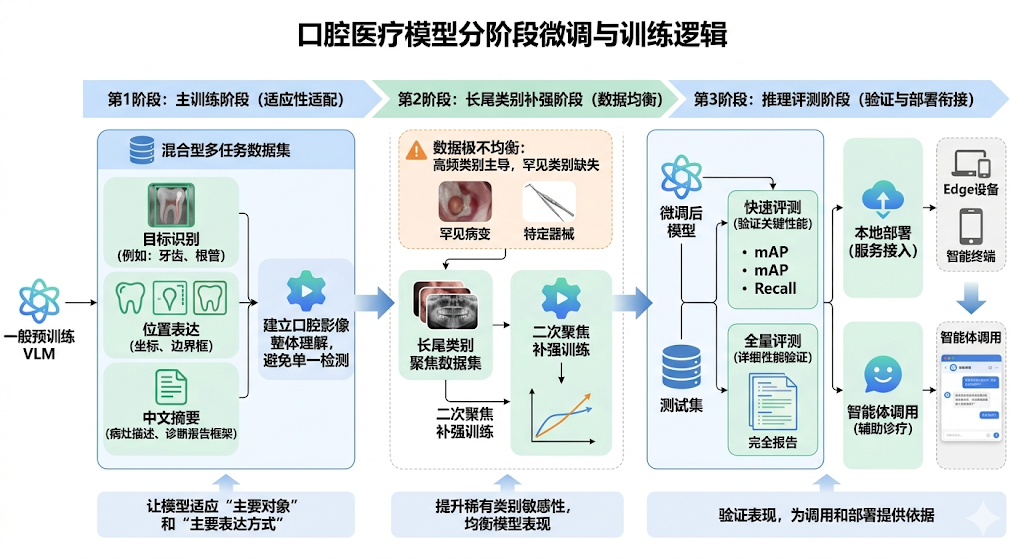
\includegraphics[width=0.96\linewidth]{oralpath-fig19-training-logic.png}
  \caption{口腔医疗模型微调与训练逻辑}
  \label{fig:oralpath-training-logic}
\end{figure}

这种设计的核心思想，是把“会识别”“会描述”和“会关注难例”拆分成相互衔接的训练目标，而不是试图在一次训练中同时解决所有问题。这样既能提升训练效率，也能使每个阶段的目标更加清晰。

\section{详细微调策略}

针对口腔医疗场景中影像长宽比特殊（全景片）、病灶细微（如早期龋齿）、专业术语复杂等挑战，本项目并不是沿用传统“单一任务、单轮训练”的方式，而是围绕口腔影像场景的特点，构建了一套面向视觉语言模型的多任务、分阶段、渐进式领域适配方案：

\subsection{训练目标}

本项目没有将微调任务限制为单一的目标检测式输出，而是将原始牙科影像标注扩展为多个层次的视觉语言学习任务。模型既需要学习“图像中有哪些目标、它们位于何处”，又需要学习“如何将这些目标组织成符合口腔场景的中文描述”，同时还需要在样本极不均衡的前提下，尽可能保留对稀有类别的识别能力。

基于这一考虑，项目将整个微调目标划分为三个互补方向：其一是结构化定位学习，其二是中文摘要表达学习，其三是长尾类别强化学习。三者并不是相互割裂的独立任务，而是在同一模型内部共同推动口腔领域能力的形成。

\subsection{训练流程安排}

在训练流程安排上，本项目采用了分阶段渐进式微调策略。

第一阶段为主体能力建立阶段，其任务重点在于让模型完成对口腔影像主要目标的识别与理解，并初步掌握中文描述方式。这一阶段并不刻意追求对所有细小类别的极致表现，而是优先建立稳定的领域基础能力，使模型先学会“看懂图像、说清结果”。

第二阶段为长尾类别补强阶段，其任务重点不再是全面学习，而是将有限训练资源集中到样本较少、但临床意义较强的类别上。

通过这种“先整体、后细节”的训练安排，可以避免模型在一开始就被复杂的类别长尾分布打乱训练节奏，同时也能够减少高频类别对低频类别的梯度压制问题。

\begin{figure}[H]
  \centering
  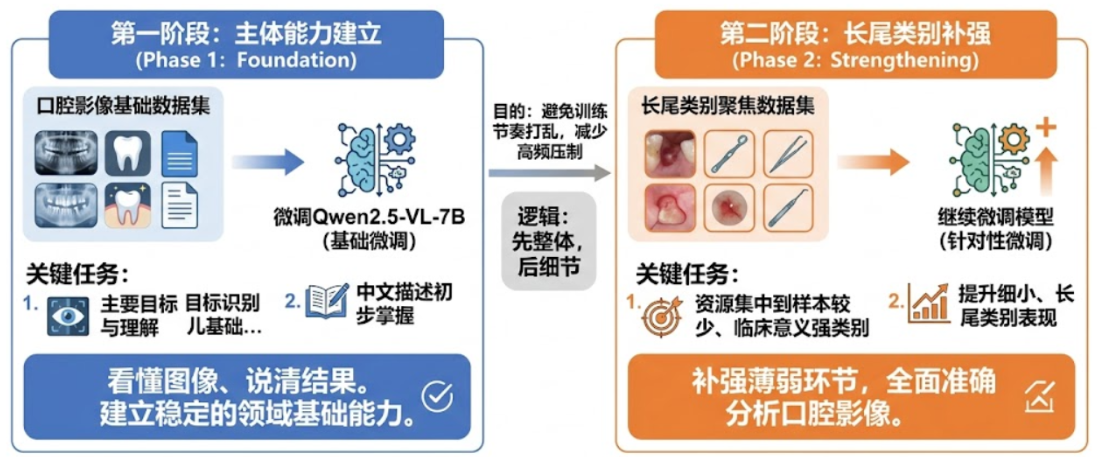
\includegraphics[width=0.96\linewidth]{oralpath-fig20-training-flow.png}
  \caption{训练流程安排}
  \label{fig:oralpath-training-flow}
\end{figure}

\subsection{具体训练方案}

在具体训练方法上，本项目采用的是 LoRA（Low-Rank Adaptation）参数高效微调方案。

相比全参数训练，LoRA 不需要对整个大模型的全部参数进行更新，而是仅在核心线性层中引入少量可训练参数，从而在尽量保留基座模型原有通用能力的同时，快速完成口腔领域知识与视觉特征的适配。

之所以采用 LoRA 而非全参数微调，一方面是考虑到多模态大模型训练成本高、工程复杂度大，另一方面也是希望在不破坏通用图文推理能力的前提下，让模型获得更稳定、更可控的专科迁移效果。LoRA 方案在训练效率、显存占用、模型可复用性以及最终权重导出方面都具有明显优势。

\begin{figure}[H]
  \centering
  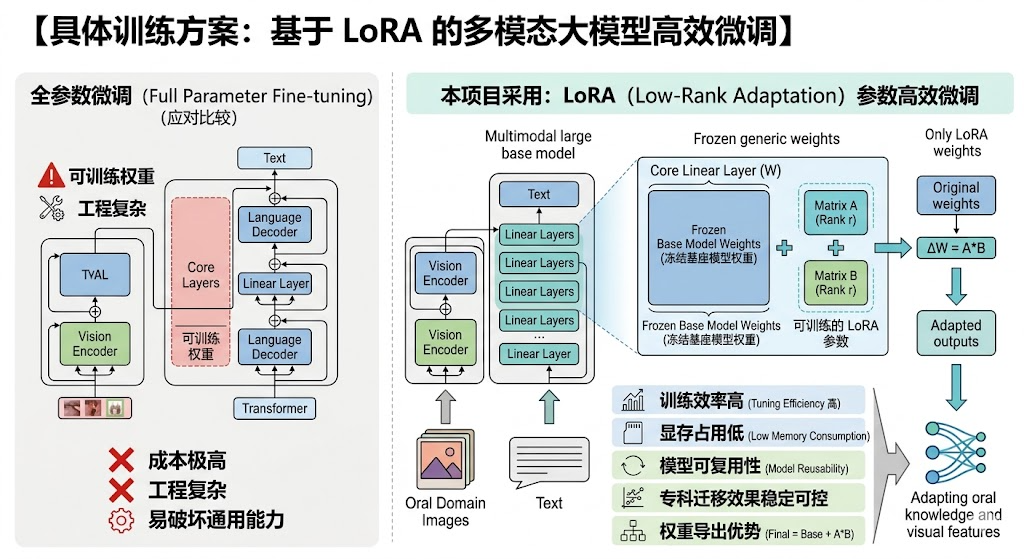
\includegraphics[width=0.96\linewidth]{oralpath-fig21-lora-scheme.png}
  \caption{基于 LoRA 的多模态大模型微调方案}
  \label{fig:oralpath-lora-scheme}
\end{figure}

\subsection{训练执行细节}

在训练执行细节上，本项目进一步结合当前硬件条件与模型特性，采用了一组面向稳定性和效率优化的训练策略。

1、混合精度计算：以降低显存占用并提高吞吐效率；

2、梯度检查点机制，以在不显著损失模型表达能力的前提下缓解长序列图文输入带来的显存压力。

3、优化器选择：优先采用 fused 版本的 AdamW，以提高训练阶段的实际执行效率。

4、输入控制：根据不同阶段任务的特点对输入长度进行区分设置：

（1）主体训练阶段保留更充分的图文上下文，确保模型能够同时处理定位信息和中文摘要信息；

（2）长尾补强阶段则适当压缩输入长度，使模型更专注于长尾类别本身，从而在有限时间内提升专项学习效率。

\subsection{创新性微调策略说明}

（一）面向多任务融合的视觉语言训练框架

本项目微调策略的一个重要创新点，在于并未简单将检测标注数据“翻译”为文本，而是把检测任务、图文摘要任务和长尾聚焦任务共同纳入统一的视觉语言训练框架中。传统检测数据集通常只能训练模型完成目标识别和位置回归，而本项目通过任务重构，使同一份牙科影像数据同时承担“目标定位监督”“中文表达监督”和“长尾类别监督”三类角色。这种设计使模型不再只具备“框出目标”的能力，而能够进一步具备“解释图像中目标及其临床含义”的能力，更符合口腔智能助手的真实使用需求。

（二）面向长尾类别的专项补强训练思路

口腔影像数据天然存在类别分布不均问题，常见修复体和常见牙列结构远多于少见病变和特殊器械。如果只依赖混合训练，模型通常会优先收敛到高频类别，对稀有类别表现不足。

针对这一问题，本项目并未仅依赖重采样或损失加权，而是进一步通过“任务级别聚焦”的方式，让模型在专门的长尾指令中只关注特定类别，从而显式强化低频目标在模型内部的表示能力。这种做法本质上是将类别不平衡问题从“样本分布问题”提升为“任务设计问题”来处理，具有较强的针对性。

（三）“主训练 + 补强训练”的层次化领域适配路径

许多传统领域微调方案会直接使用全部数据进行统一训练，但这种做法在面对复杂多模态任务时，往往容易造成模型在训练早期目标不清、学习方向混杂。本项目将“主体能力构建”和“长尾能力强化”明确拆分为不同阶段，使模型在主训练阶段优先获得稳定的口腔影像识别与表达基础，再在第二阶段补足其对少样本类别的关注能力。这样的安排不仅提高了训练的可解释性，也更有利于控制不同阶段的目标与风险。

\begin{figure}[H]
  \centering
  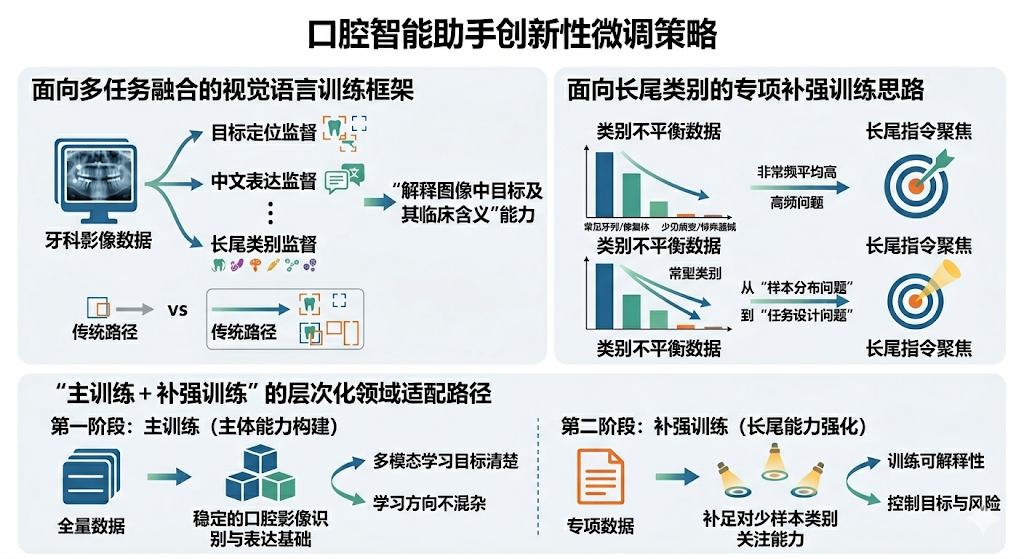
\includegraphics[width=0.96\linewidth]{oralpath-fig22-innovation-strategy.png}
  \caption{创新性微调策略说明}
  \label{fig:oralpath-innovation-strategy}
\end{figure}

总体来看，本项目的详细微调策略可以概括为：以高质量通用视觉语言模型为基座，以口腔影像多任务指令数据为训练核心，以 LoRA 为主要适配方式，以分阶段训练和长尾补强为优化重点，以部署可落地为最终导向。这一策略既兼顾了口腔场景下的识别精度与表达能力，也兼顾了当前实验资源约束、训练周期控制和后续部署实施的现实要求。

\section{微调结果自测及说明}

为验证模型在口腔场景下的实际适配效果，项目团队在主训练完成后，依次对模型进行了训练过程自检、长尾类别补强验证以及多轮快速评测。

考虑到本项目的训练目标并不单一，既包含结构化定位任务，也包含中文摘要任务，因此在结果验证阶段没有仅依赖通用文本相似度指标，而是结合任务特点分别采用了训练损失、验证损失、文本类指标和结构化指标进行综合分析，尽可能从“模型是否稳定收敛”“模型是否具备口腔领域表达能力”“模型是否真正学会结构化识别”三个层面，对当前模型效果作出较全面判断。

\subsection{训练收敛情况}

在训练流程上，模型首先完成了主训练阶段，再完成了长尾类别补强阶段。主训练阶段面向多任务混合数据展开，重点学习口腔影像中的主体目标识别能力和中文摘要表达能力；长尾补强阶段则聚焦于稀有类别，进一步增强模型对少样本病变和器械目标的敏感性。当前训练结果表明，两阶段训练整体过程是稳定的，未出现明显的发散或训练崩溃现象。

主训练阶段共完成 2410 个优化步，最佳验证点出现在 checkpoint-2000，其最佳验证损失为 0.2144，最终训练损失约为 0.2572。

从训练曲线看，损失值整体呈下降趋势，说明模型已经较稳定地完成了从通用多模态基座向口腔场景的主体能力迁移。

长尾补强的第二轮训练共完成 99 个优化步，最佳验证点出现在 checkpoint-50，对应的验证损失约为 0.3955，最终训练损失约为 0.4098。由于长尾补强阶段的数据分布更稀疏、任务目标更聚焦，因此其损失数值不能简单与主训练阶段横向比较，但从训练日志和收敛趋势看，该阶段同样保持了稳定优化，没有出现明显的过拟合失控现象。

\subsection{评测策略说明}

由于本项目的训练数据同时包含结构化定位任务、中文摘要任务和长尾类别聚焦任务，因此单一评测方式很难完整反映模型能力。项目团队在评测阶段采取了“两层评测”的思路。

1、基于文本相似度的快速评测，用于观察模型整体输出是否已经偏离参考答案；

2、面向任务本身的结构化评测，用于更准确判断模型在 JSON 输出、类别识别、目标匹配和中文摘要等方面的真实表现。

其中，结构化评测是当前最值得参考的一组结果。原因在于，检测型任务和长尾聚焦任务本质上都要求模型输出可解析的结构化 JSON，如果只使用 ROUGE 或 Token F1 来评价，容易低估模型在类别和位置上的真实能力，也容易因为字段顺序变化而误判结果。因此，本项目对 detection\_json 和 rare\_focus\_json 任务采用了更贴合任务的指标：包括 JSON 可解析率、结构化完全匹配率、类别识别 F1、目标数量误差、IoU 条件下的检测精度与召回率，以及已命中目标的平均 IoU。同时，对 summary\_zh 任务保留文本相似度指标，用于评估模型的中文摘要表达能力。

\begin{figure}[H]
  \centering
  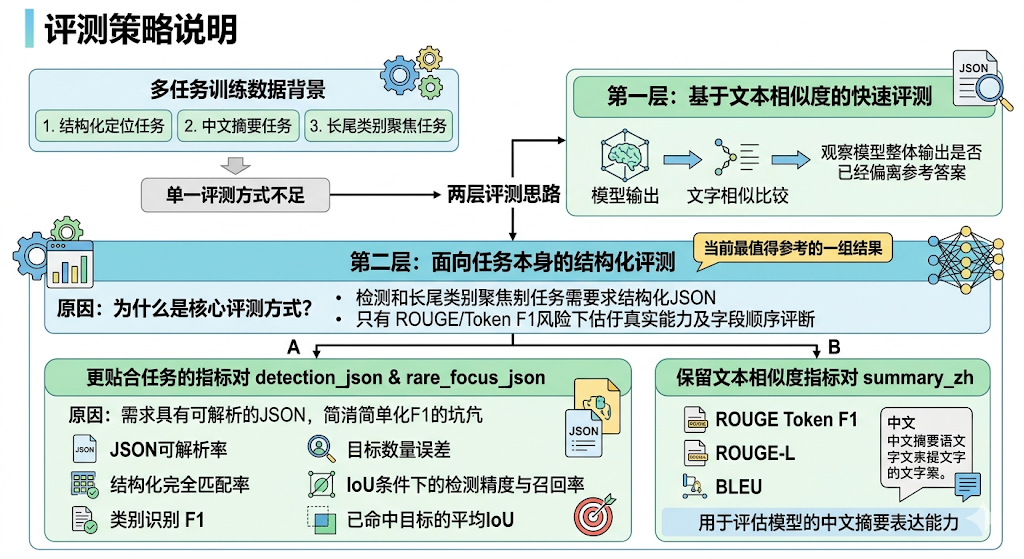
\includegraphics[width=0.96\linewidth]{oralpath-fig23-evaluation-strategy.png}
  \caption{评测策略说明}
  \label{fig:oralpath-evaluation-strategy}
\end{figure}

\subsection{口腔 X 片中文摘要能力评测}

为了验证 OralPath 在口腔影像场景中的实际应用能力，项目团队重点对模型的口腔 X 片中文摘要生成能力进行了专项评测。之所以将这一能力单独抽出进行分析，是因为在口腔临床场景中，医生对于模型的需求并不只是“识别出图中某个目标”，而更希望模型能够对整张影像中的主要发现进行归纳、提炼并用符合医学语义的中文表达出来。

相比单纯的结构化框输出，口腔 X 片摘要能力更接近实际应用中“图像辅助解读”的使用需求，也是 OralPath 当前最具代表性的优势能力之一。

\begin{figure}[H]
  \centering
  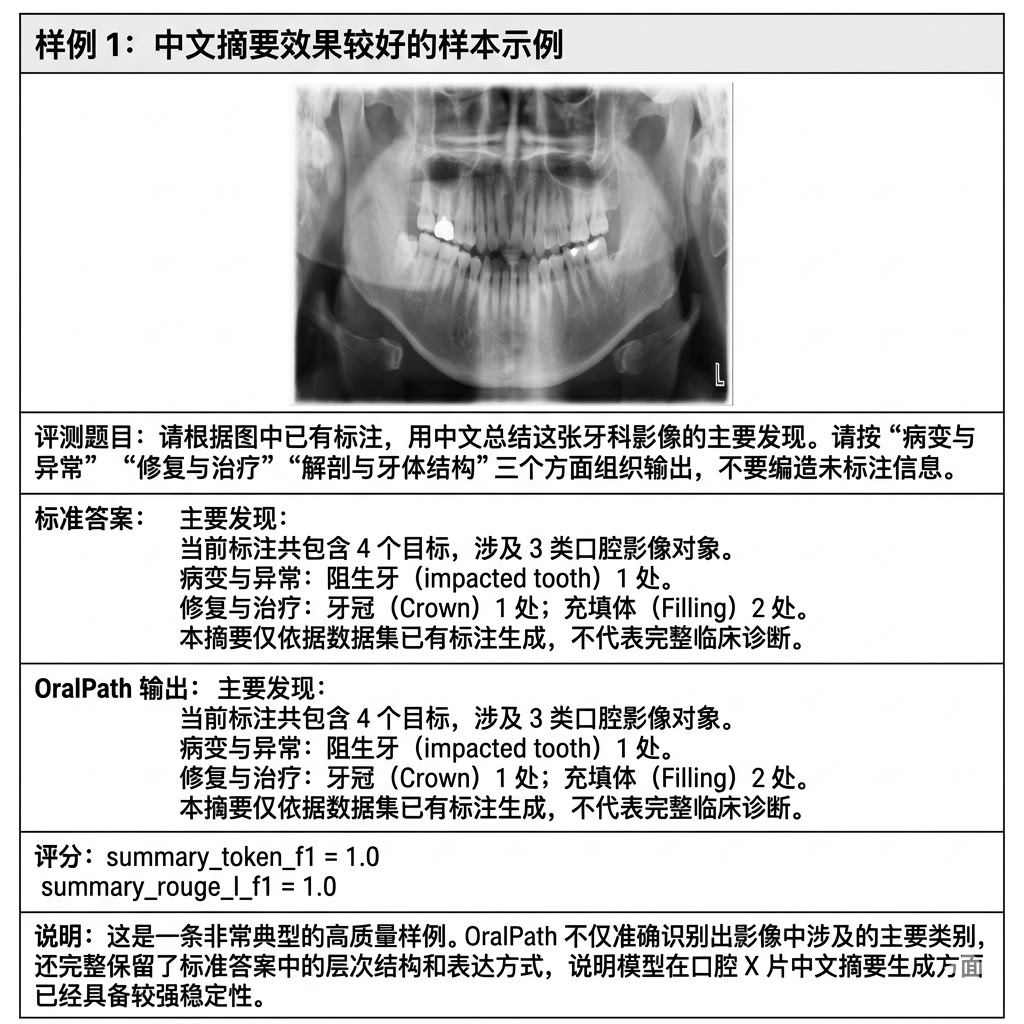
\includegraphics[width=0.96\linewidth]{oralpath-fig24-summary-example.png}
  \caption{中文摘要样例示意}
  \label{fig:oralpath-summary-example}
\end{figure}

当前结果显示，OralPath 在中文摘要任务上的 \softid{token\_f1\_mean} 达到 0.6511，\softid{rouge\_l\_f1\_mean} 达到 0.6461。这一结果说明，模型已经能够较稳定地抓住口腔 X 片中的主要语义内容，并以较接近参考答案的方式完成中文总结。

从输出表现来看，OralPath 在摘要任务中的优势主要体现在两个方面：

对主要口腔对象和异常征象的抓取能力较强。模型能够识别并整合龋坏、阻生牙、根尖周病变、充填体、牙冠、根管治疗等高频目标，并在输出中形成较清晰的“主要发现”描述。这意味着模型已经建立起对口腔影像中核心语义元素的优先感知能力。

中文表达结构较稳定。在多条测试样本中，OralPath 能够较好地沿用“病变与异常—修复与治疗—解剖与牙体结构”的组织方式输出摘要，使结果更符合面向临床和教学场景的表达习惯。相比原始基座模型，这一能力提升尤为明显，因为未经微调的通用模型虽然能够处理图文输入，但难以稳定地产出口腔场景所需的专业化中文总结，而 OralPath 已经表现出较明显的专科表达优势。

从口腔影像任务的复杂性来看，这一结果具有较强的实际意义。因为牙科全景片通常同时包含牙体、牙列、修复结构、病变影像及相关解剖特征，信息密度高，类别繁多，而 OralPath 已能够在这种复杂图像中提炼出关键信息，并形成面向中文场景的较完整表达，这说明 OralPath 经过口腔专向微调后，已经不再只是一个通用视觉语言模型，而是初步具备了口腔影像语义归纳能力。

\subsection{口腔 X 片主要对象识别能力评测}

除了中文摘要能力之外，口腔 X 片中的主要对象识别能力也是 OralPath 当前多模态能力的重要组成部分。

对于口腔影像场景而言，模型不仅需要能够“总结这张图的大致发现”，还需要具备对核心牙科目标进行区分和定位的能力，例如识别充填体、牙冠、阻生牙、根管治疗相关结构、缺失牙以及部分病变征象等。这种能力虽然不同于传统目标检测模型的严格框回归任务，但在口腔多模态助手的实际应用中依然至关重要，因为模型是否能够识别主要对象，直接决定了其后续摘要、问答和诊疗辅助推理的质量。

\begin{figure}[H]
  \centering
  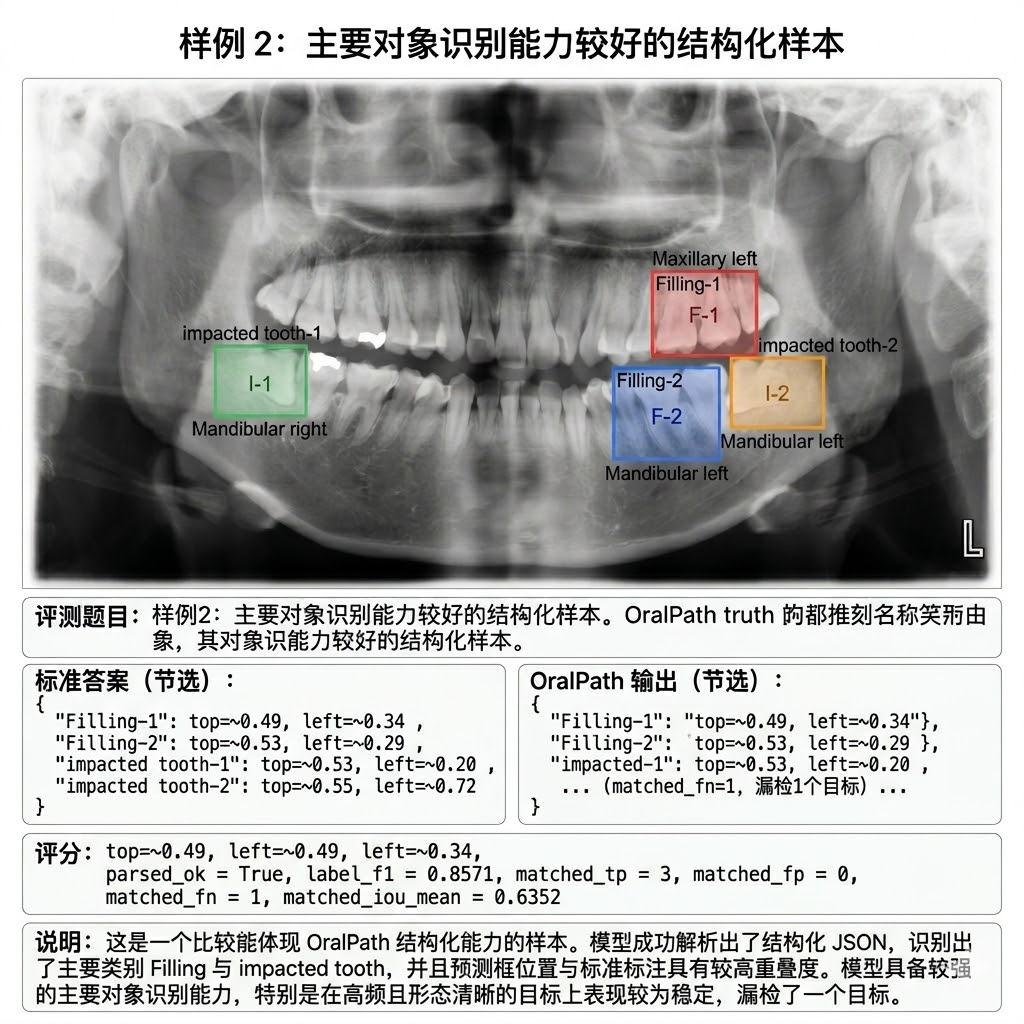
\includegraphics[width=0.96\linewidth]{oralpath-fig25-detection-example.png}
  \caption{对象识别能力较好的结构化样本示意}
  \label{fig:oralpath-detection-example}
\end{figure}

在当前项目中，团队采用了面向结构化输出的专门评测方式，对 OralPath 在牙科主要对象识别任务中的表现进行了验证。评测不是简单使用通用文本相似度打分，而是围绕结构化结果本身进行分析，包括 JSON 可解析率、类别识别 F1、目标数量误差、IoU 条件下的精度与召回率，以及匹配成功目标的平均 IoU。通过这种更贴近实际任务的方式，能够更真实地反映模型在“主要对象识别”上的能力基础。

\begin{table}[H]
  \centering
  \caption{评测项目与模型的表现}
  \label{tab:oralpath-current-metrics}
  \small
  \renewcommand{\arraystretch}{1.18}
  \begin{tabularx}{\linewidth}{p{0.28\linewidth}p{0.18\linewidth}X}
    \toprule
    指标 & OralPath 当前结果 & 说明 \\
    \midrule
    \softid{json\_parse\_rate} & 0.5417 & 超过一半的结构化结果已经可以被系统直接解析 \\
    \softid{label\_f1\_mean} & 0.3577 & 模型已经具备一定的主要牙科对象识别能力 \\
    \softid{det\_precision\_iou50} & 0.3886 & 模型输出目标较保守，但命中的目标准确性尚可 \\
    \softid{det\_recall\_iou50} & 0.0642 & 当前主要短板在于多目标场景下的召回不足 \\
    \softid{det\_f1\_iou50} & 0.1102 & 结构化识别能力已建立基础，但整体仍有较大提升空间 \\
    \softid{matched\_iou\_mean} & 0.6449 & 对成功命中的目标，定位框质量较好 \\
    \bottomrule
  \end{tabularx}
\end{table}

当前评测结果表明，OralPath 在主要对象识别任务上已经具备一定基础。其 \softid{label\_f1\_mean} 为 0.3577，说明模型已经能够在相当一部分样本中识别出图像中的主要牙科对象类别；\softid{json\_parse\_rate = 0.5417}，说明超过一半的结构化结果已经可以直接被解析；而 \softid{matched\_iou\_mean = 0.6449} 则表明，在成功命中的目标上，预测框与参考框之间具有较好的重叠度，定位质量总体较可靠。从这些指标可以看出，当前 OralPath 并不是“不能识别目标”，而是已经建立起了对主要牙科对象的初步识别能力，特别是在高频目标和形态较清晰的对象上表现相对稳定。

可见 OralPath 在口腔 X 片主要对象识别任务上已经较好能力。模型不仅能够识别充填体、牙冠、阻生牙、根管治疗等高频牙科对象，而且在命中目标时具有较好的定位质量，\softid{matched\_iou\_mean} 达到 0.6449。虽然当前在多目标密集场景下仍存在召回偏低的问题，但与原始基座模型相比，OralPath 已经表现出明确的口腔结构识别优势，为图像问答和摘要生成提供了稳定的对象级视觉基础。

\subsection{原始基座模型与微调模型对比}

\begin{table}[H]
  \centering
  \caption{模型微调前后结构化任务对比}
  \label{tab:oralpath-structured-before-after}
  \small
  \renewcommand{\arraystretch}{1.18}
  \begin{tabularx}{\linewidth}{p{0.26\linewidth}p{0.27\linewidth}p{0.24\linewidth}X}
    \toprule
    指标 & 原始 Qwen2.5-VL-7B-Instruct & 当前微调模型（OralPath） & 变化 \\
    \midrule
    JSON 可解析率 & 1.0000 & 0.6538 & 下降 \\
    完全结构匹配率 & 0.0000 & 0.1538 & 上升 \\
    类别识别 F1 & 0.0000 & 0.4438 & 明显上升 \\
    目标数量误差 & 5.6538 & 5.3462 & 略有改善 \\
    检测精度 & 0.0000 & 0.3830 & 明显上升 \\
    检测召回 & 0.0000 & 0.0978 & 明显上升 \\
    检测综合 F1 & 0.0000 & 0.1558 & 明显上升 \\
    匹配框平均 IoU & 0.0000 & 0.6347 & 明显上升 \\
    \bottomrule
  \end{tabularx}
\end{table}

\begin{table}[H]
  \centering
  \caption{模型微调前后摘要任务对比}
  \label{tab:oralpath-summary-before-after}
  \small
  \renewcommand{\arraystretch}{1.18}
  \begin{tabularx}{\linewidth}{p{0.26\linewidth}p{0.27\linewidth}p{0.24\linewidth}X}
    \toprule
    指标 & 原始 Qwen2.5-VL-7B-Instruct & 当前微调模型（OralPath） & 变化 \\
    \midrule
    \softid{token\_f1\_mean} & 0.0000 & 0.6685 & 显著提升 \\
    \softid{rouge\_l\_f1\_mean} & 0.0000 & 0.6660 & 显著提升 \\
    \bottomrule
  \end{tabularx}
\end{table}

原始 Qwen2.5-VL-7B-Instruct 作为通用视觉语言基座模型，虽然具备较强的通用图文理解能力，但由于未经过口腔专科数据和本项目任务格式的适配，在当前结构化牙科识别与中文摘要评测协议下，几乎无法产生有效得分。尤其在类别识别、检测匹配和摘要生成等指标上接近于零，这并不说明基座模型通用能力不足，而是说明其尚未形成针对口腔场景的专科任务能力。与之相比，经过领域微调后的 OralPath 在相同协议下已能够获得显著更高的结果，体现出明确的口腔专科适配效果。

\section{微调效果总结}

综上所述，本项目通过引入多任务融合的微调策略，成功地将通用视觉语言模型转化为专门适配口腔影像的多模态模型，显著提高了口腔影像的目标识别、结构化定位和中文摘要生成能力。通过长尾类别补强、分阶段训练和 LoRA 微调等策略，模型不仅提升了在高频目标上的表现，也显著增强了对低频类别的敏感性。

尽管仍有一些挑战需要克服，但 OralPath 已在多个方面表现出良好的临床应用潜力，并为口腔医疗领域的智能化辅助诊疗提供了可行的技术路径。

同时，本团队决定在比赛结束后将模型及数据集开源，解决市面上缺乏真正开源的牙科影像模型、大规模牙科影像数据集的痛点。

% !TeX root = ../main.tex

\chapter{学习画像}
\label{sec:profile-path}

\section{学习画像总体架构}

口腔医学学习具有知识依赖密集、概念边界细致、诊疗决策链条长的特点。同一疾病的知识点下往往同时涉及解剖基础、病因机制、临床表现、诊断依据、治疗原则和预后维护。OralSage 因此将学习画像设计为贯穿学习过程的共享状态模型，用于连接课程规划、讲授组织、上下文问答、阶段测评和学习计划推荐。画像记录学习者当前希望达成的目标，也记录系统在交互中逐步观察到的知识状态、解释偏好和执行节奏，使每一次后续决策都能建立在可复用的个体信息之上。

参考智能教学系统中学习者建模与知识追踪的基本思想\cite{corbett1994knowledge,vanlehn2011relative}，与近期智能体个性化辅导研究中“静态知识基础+动态个人记忆”的分层理念\cite{deeptutor2026}，OralSage 以口腔医学知识图谱组织课程知识与学习单元，以学习事件和多层记忆记录学习者的学习行为，并在持续交互中动态更新学习画像。面向具体学习任务时，系统再通过角色化画像切片，将与当前主题和 Agent 职责相关的信息按需交付，为课程规划、讲解、答疑、测评和计划推荐提供个性化依据。

\begin{figure}[H]
  \centering
  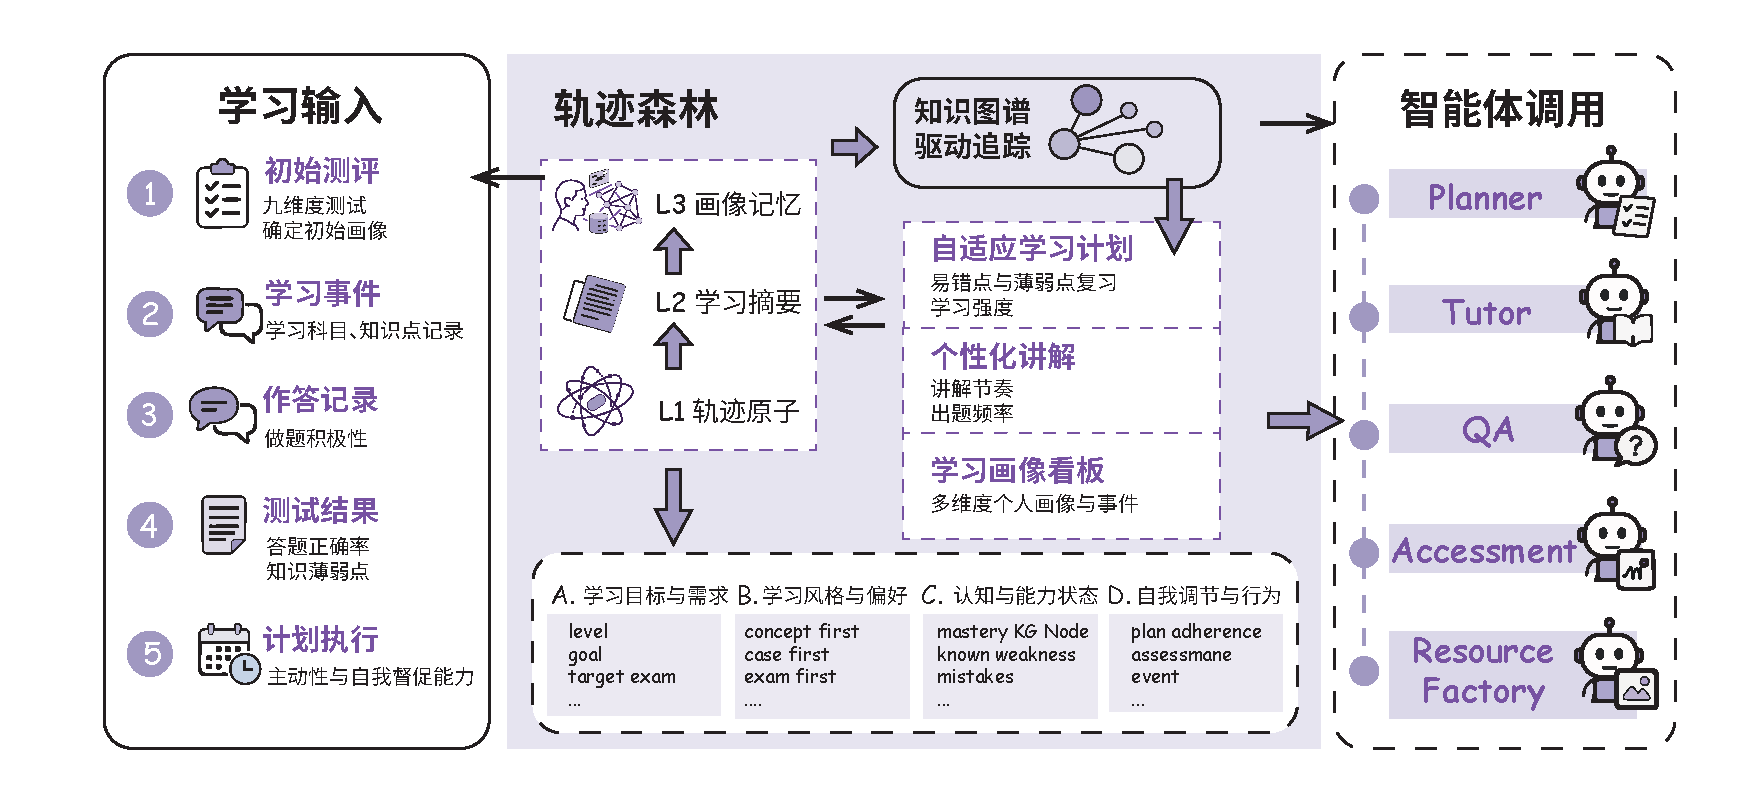
\includegraphics[width=\linewidth]{figures/profile-overall-architecture.pdf}
  \caption{OralSage 学习画像总体架构}
  \label{fig:profile-overall-architecture}
\end{figure}

如图\ref{fig:profile-overall-architecture}所示，OralSage 将初始测评、课程讲授、追问、答题、阅读、复习和计划打卡等学习事件存入持久化学习记忆中，经由按学习轨迹聚合的摘要形成较为稳定的行为描述，最终通过 LLM 总结写入长期记忆，形成动态更新的学习画像，并且支持产品侧的响应速度与长期行为建模保持协同。

\section{初始画像构建与教学调节}

\subsection{初始测评}

学习者首次进入学习流程时，OralSage 将提供九道测评题目，围绕学习目标、每日可用时间、知识进入方式、讲解深度、学习节奏、小测接受度、计划引导需求、时间紧张时的优先策略和自动调整接受度几个维度来采集用户的偏好信息，为个性化服务提供基础。测评结果写入基础画像，并生成解释深度、知识进入方式、互动倾向、节奏和计划支持需求等风格维度。系统据此生成考试导向、练习驱动、病例驱动、机制推导等学习者类型描述。

\begin{table}[H]
  \centering
  \caption{初始测评维度与学习调节映射}
  \label{tab:onboarding-profile-mapping}
  \begin{tabularx}{\linewidth}{p{0.22\linewidth}p{0.30\linewidth}X}
    \toprule
    测评维度 & 主要画像字段 & 后续调节作用 \\
    \midrule
    学习目标 & 学习目标、目标考试 & 路径重点与任务优先级 \\
    每日时间 & 每日可用时间、节奏 & 每日任务量与计划周期 \\
    知识进入方式 & 讲解偏好、进入方式 & 概念、病例、题目和考点的组织顺序 \\
    讲解深度 & 解释深度 & 机制讲解与要点归纳的展开程度 \\
    小测接受度 & 测评偏好 & 小测密度与阶段练习安排 \\
    计划引导需求 & 计划支持需求 & 任务拆分粒度与推荐强度 \\
    时间紧张策略 & 复习需求、目标倾向 & 重点复习与主线推进的权重 \\
    自动调整接受度 & 执行节奏、计划偏好 & 计划变更的呈现方式与调整频率 \\
    \bottomrule
  \end{tabularx}
\end{table}

\subsection{面向口腔医学任务的支架化调节}

支架化教学与维果茨基提出的“最近发展区”思想密切相关，强调辅导系统应依据学习者的当前状态提供适度支持，并随着学习进展调整支持强度\cite{wood1976tutoring}。OralSage 将这一思想落实为共享学习状态驱动的协同调节机制。系统在课程范围、知识点优先级、讲解组织、答疑补充、测评反馈和任务密度等决策中读取同一份学习画像，根据学习目标确定课程重点，根据知识掌握状态调整讲解与复习内容，并结合可用时间和执行节奏调节任务密度，使不同学习环节围绕学习者当前状态保持协调，并在后续交互中持续调整支持方式。

OralSage 的这种动态调节将学习偏好视为可被持续校准的工作假设。用户后续的追问方式、答题反馈和计划执行能够逐渐补充对学习行为的理解，并逐步形成更加稳定的学习画像。因此，系统能够在较短学习任务中保持一致的讲解策略，也能够在跨会话学习中根据长期表现调整节奏和任务密度。

\section{轨迹森林与多层学习记忆}

\subsection{从学习事件到长期画像}

为处理跨课程、跨会话的连续学习记录，OralSage 构建了“轨迹森林”式的多层学习记忆。系统将学习者在不同课程和会话中产生的学习事件分别组织为持续延伸的学习轨迹，多条轨迹共同构成反映长期学习过程的“轨迹森林”。该结构围绕问答、讲授、测评、规划、阅读、复习和学习计划等学习行为，将细粒度的事件逐步归纳为可调用的长期状态。L1、L2 与 L3 的层级关系如图\ref{fig:trace-forest-flow}所示。

\textbf{L1 学习轨迹原子层}以 \texttt{lesson\_events} 保存课程学习、授课推进、用户追问、答题提交、进度更新、资源阅读、复习完成和计划执行等学习事件，并关联 KG 节点、行为结果和上下文信息。

\textbf{L2 学习摘要层}以 \texttt{learning\_summaries} 对同类事件进行阶段性归纳。摘要能够捕捉画像关键变化、关联 KG 节点和来源事件编号，避免下游模块反复读取大量原始交互记录。\texttt{memory\_consolidation\_meta} 保存已处理事件的位置，使归纳过程可按新增事件持续推进。

\textbf{L3 长期画像记忆层}将阶段性摘要和有效学习行为整理为六个维度的画像字段，分别覆盖总体特征、知识掌握、薄弱点、学习偏好、目标和节奏。\texttt{profile\_state} 进一步汇总学习风格、薄弱点与易错点、知识点掌握度和个性化策略。

\begin{figure}[H]
  \centering
  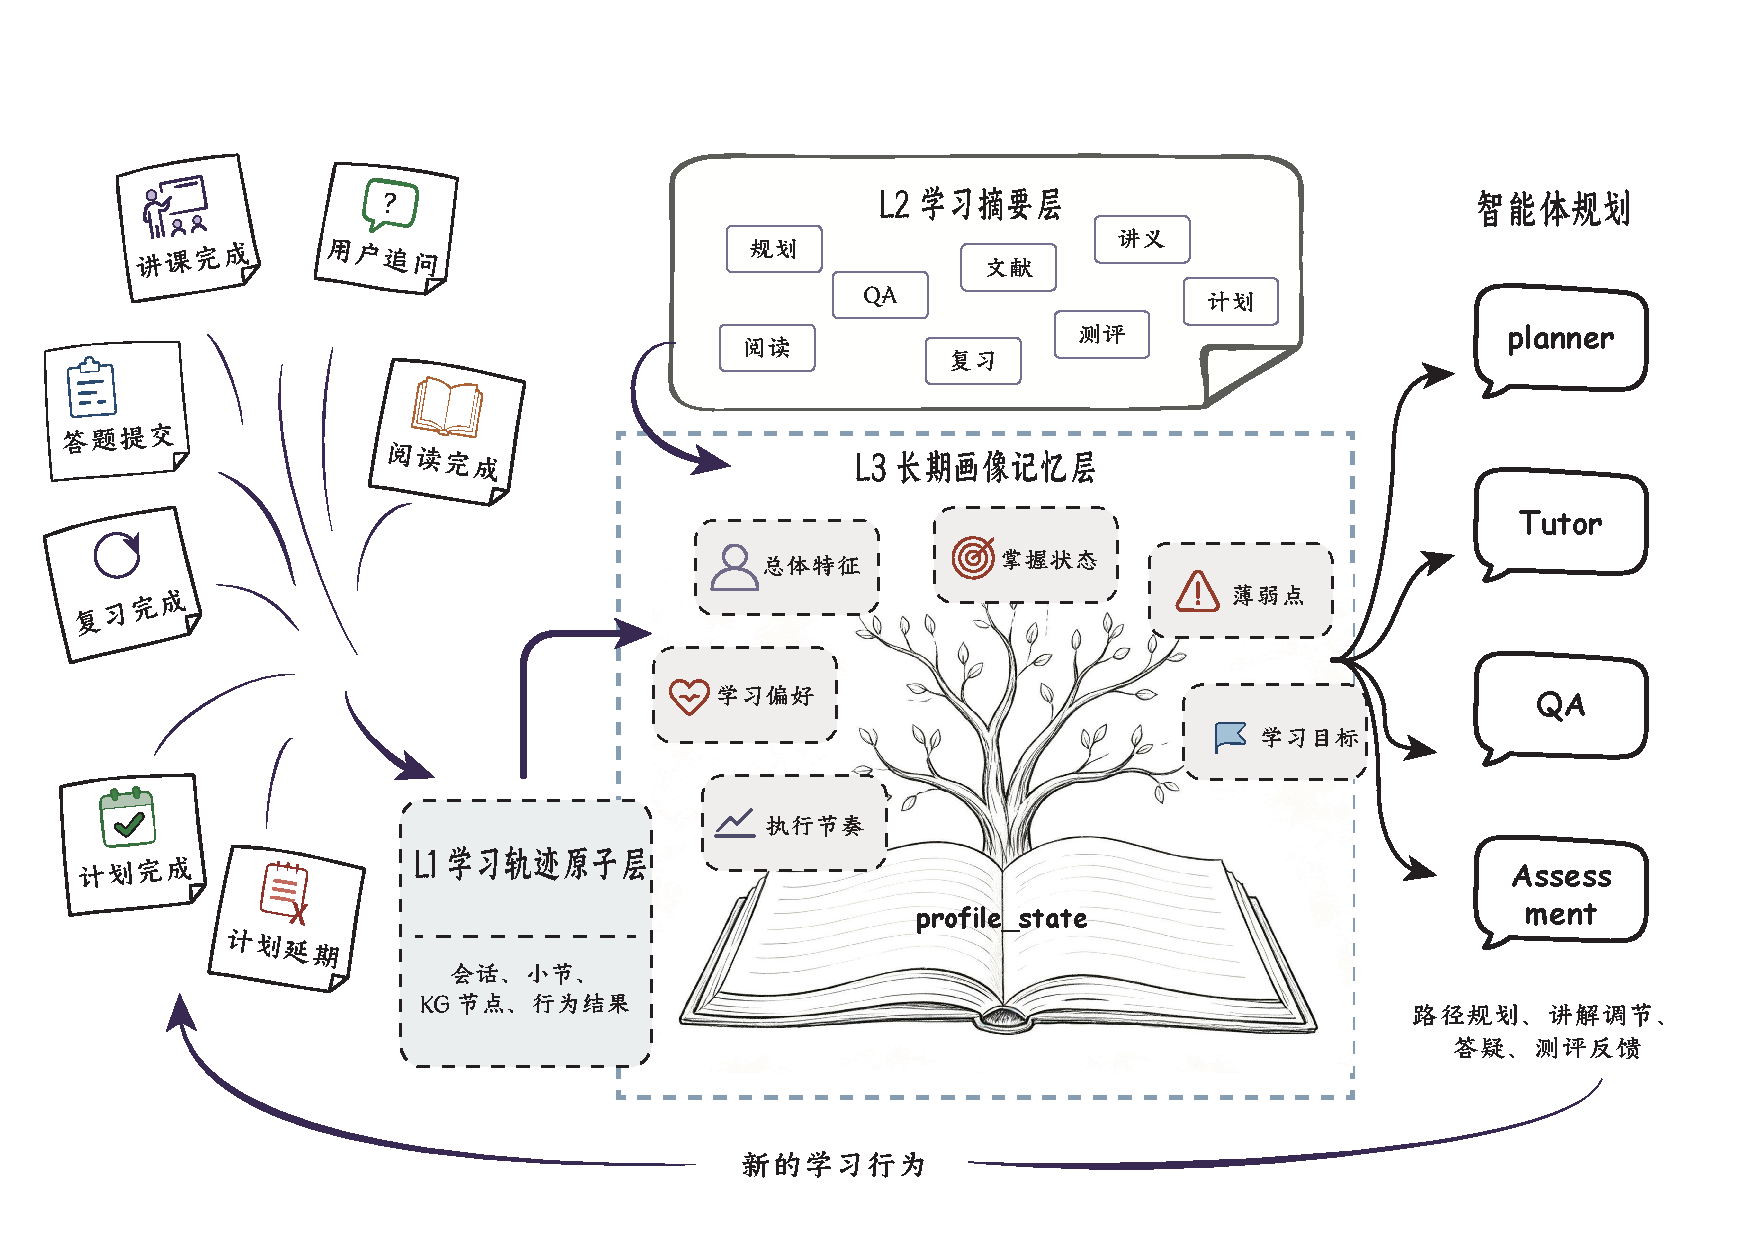
\includegraphics[width=0.96\linewidth]{figures/trace-forest.pdf}
  \caption{轨迹森林三层协作流程}
  \label{fig:trace-forest-flow}
\end{figure}

\subsection{学习画像的动态更新}

OralSage 能够将“用户说过什么”“用户做过什么”“据此形成何种判断”和“用户是谁”连接为完整的记录链。学习事件存入 L1 后，系统对事件进行语义归类，记录相应的记忆类别、画像维度、行为内容和关联 KG 节点；随后通过事件编号与有效性校验，将同类事件逐步归纳为阶段性摘要。只有经过持续学习行为支持、能够形成相对稳定判断的信息，才会进一步进入长期画像。长期画像中的特征并非一次写入后永久固定，而是能够随着后续行为被新增、修订、强化或减弱。对于掌握度与薄弱点，系统会保存用户答题分值，并结合后续学习表现更新相关知识点的掌握状态与错误理解程度。

\subsection{数字问诊事件与画像反馈}

数字问诊使用独立事件类型记录临床训练轨迹。\texttt{clinical\_speaking\_started} 保存病例训练启动信息，\texttt{clinical\_diagnosis\_confirmed} 保存诊断确认结果，\texttt{clinical\_speaking\_answer\_assessed} 记录病理机制、临床表现与诊断依据、鉴别诊断、治疗原则、风险与随访的分项得分，\texttt{clinical\_speaking\_completed} 汇总总分与完成状态。这些事件在画像时间线中以“问诊、诊断、考核”呈现，学习者可以通过问诊筛选查看相关活动。

判官 Agent 的分项结果会更新相关知识节点的掌握度、接触次数和置信度，回答中遗漏的关键内容同步进入已知薄弱点。画像保留目标诊断、领域名称、得分、遗漏要点和会话来源，使一次表达不足能够定位到具体知识内容。新建问诊会话时，病例选择服务读取 \texttt{known\_weak\_points} 与近期学习主题，将已有学习记录转化为优先训练方向，完成“训练表现、画像变化、再次选题”的连续循环。

由于学习目标、可用时间、讲解偏好和任务执行策略会随课程阶段发生变化，OralSage 将这一现象建模为\textbf{学习偏好漂移}（learner preference drift），并据此构建时变学习者画像。时间感知推荐研究表明，用户兴趣与行为模式具有明显的时间动态，较早观察对当前偏好的解释力会逐步减弱\cite{koren2009temporal}。在口腔医学学习场景中，系统学习、考前冲刺和查缺补漏等阶段对内容组织与任务密度的需求并不相同，因此画像聚合需要持续关注近期学习行为，该设计能够降低一次短暂偏好对长期画像的影响，同时保留反复出现的稳定行为特征。

设某条记忆距当前时间为 $\Delta t$ 天，其时间权重定义为：
\begin{equation}
  w_t=\max\left(0.25,\ 0.5^{\Delta t/90}\right).
  \label{eq:profile-recency}
\end{equation}

其中，画像信号的减半周期设置为90天，使置信度与时间权重共同影响风格和状态的汇总，并通过 0.25 的下界保留长期目标、持续性薄弱点和稳定偏好的基础影响，适合处理学习者在备考冲刺、课程切换等场景中的短期行为波动。

\section{角色画像切片与 Agent 调用}

完整学习画像包含较多历史信息，若所有模块都读取全部内容，会显著增加上下文负担，也会导致当前任务最关心的部分被淹没。因此，OralSage 构建 Profile Slice 机制。系统根据Agent角色、当前主题、小节和关联 KG 节点提取小型画像子集，并优先保留与当前知识节点相关的掌握度和薄弱点记录。存在会话上下文时，切片还会附带近期学习摘要，使智能体能够理解当前学习阶段。具体按需调用的画像切片内容与决策影响如表\ref{tab:profile-slices-agents}所示。

\begin{table}[H]
  \centering
  \caption{智能体的画像切片与决策影响}
  \label{tab:profile-slices-agents}
  \begin{tabularx}{\linewidth}{p{0.18\linewidth}p{0.42\linewidth}X}
    \toprule
    调用模块 & 主要切片内容 & 决策影响 \\
    \midrule
    Planner & 目标、每日时间、节奏、薄弱点、KG 节点掌握度、近期学习摘要 & 路径范围、小节顺序、任务密度与复习插入位置 \\
    Tutor & 解释偏好、知识进入方式、节奏、当前节点掌握度与薄弱点 & 讲解入口、例证组织、展开深度和小测提示 \\
    QA & 近期困惑、表达偏好、相关 KG 节点、掌握度与薄弱点 & 答疑角度、补充解释范围和是否需要加强复习 \\
    Assessment & 答题历史、错因摘要、薄弱点、掌握度与节奏 & 评分反馈、错因解析和补救建议 \\
    综合考试工具 Agent & 薄弱知识点、掌握记录、近期作答表现与目标考试 & 单选题优先级、简答题知识侧重与复习内容更新 \\
    Study-Planner & 掌握状态、待完成任务、延期记录、错题记录和执行节奏 & 继续学习、复习、练习、自测和补计划任务 \\
    \bottomrule
  \end{tabularx}
\end{table}

综合考试调用画像切片时，仅保留与命题有关的知识状态和学习目标。服务依据这些信息优先选择与薄弱内容相关的题库题目，并将同一份切片作为讯飞星火生成简答题时的知识侧重信息。考试结果中的单选得分、简答题反馈和缺失要点随后进入学习记录，后续复习推荐能够读取这一轮考试留下的细粒度表现。

\section{知识图谱约束的知识状态追踪}

知识追踪的关键在于将学习行为映射到明确的知识单元，并持续更新该单元的掌握状态\cite{corbett1994knowledge,piech2015deep}。OralSage 以口腔医学知识图谱节点作为课程学习单元，将课程大纲、讲义小节、题库和学习事件通过 KG 节点关联到同一知识空间，使“系统已讲授的内容”“用户作答的题目”“用户反复追问的概念”能够在同一节点尺度上汇合。

当前实现采用面向业务可解释性的掌握记录机制。系统围绕用户、会话和 KG 节点汇聚讲授覆盖、测评作答与问答困惑等学习信息，并在 \texttt{mastery\_records} 及直接问答掌握记录中保存掌握分数、置信度、讲授次数和关联上下文。各类行为依据其诊断价值写入不同幅度的状态增量，明确困惑同步进入薄弱点记录。该机制将分散的学习过程收束为节点级知识状态，为后续复习推荐、定向练习和个性化答疑提供统一输入。

\begin{figure}[H]
  \centering
  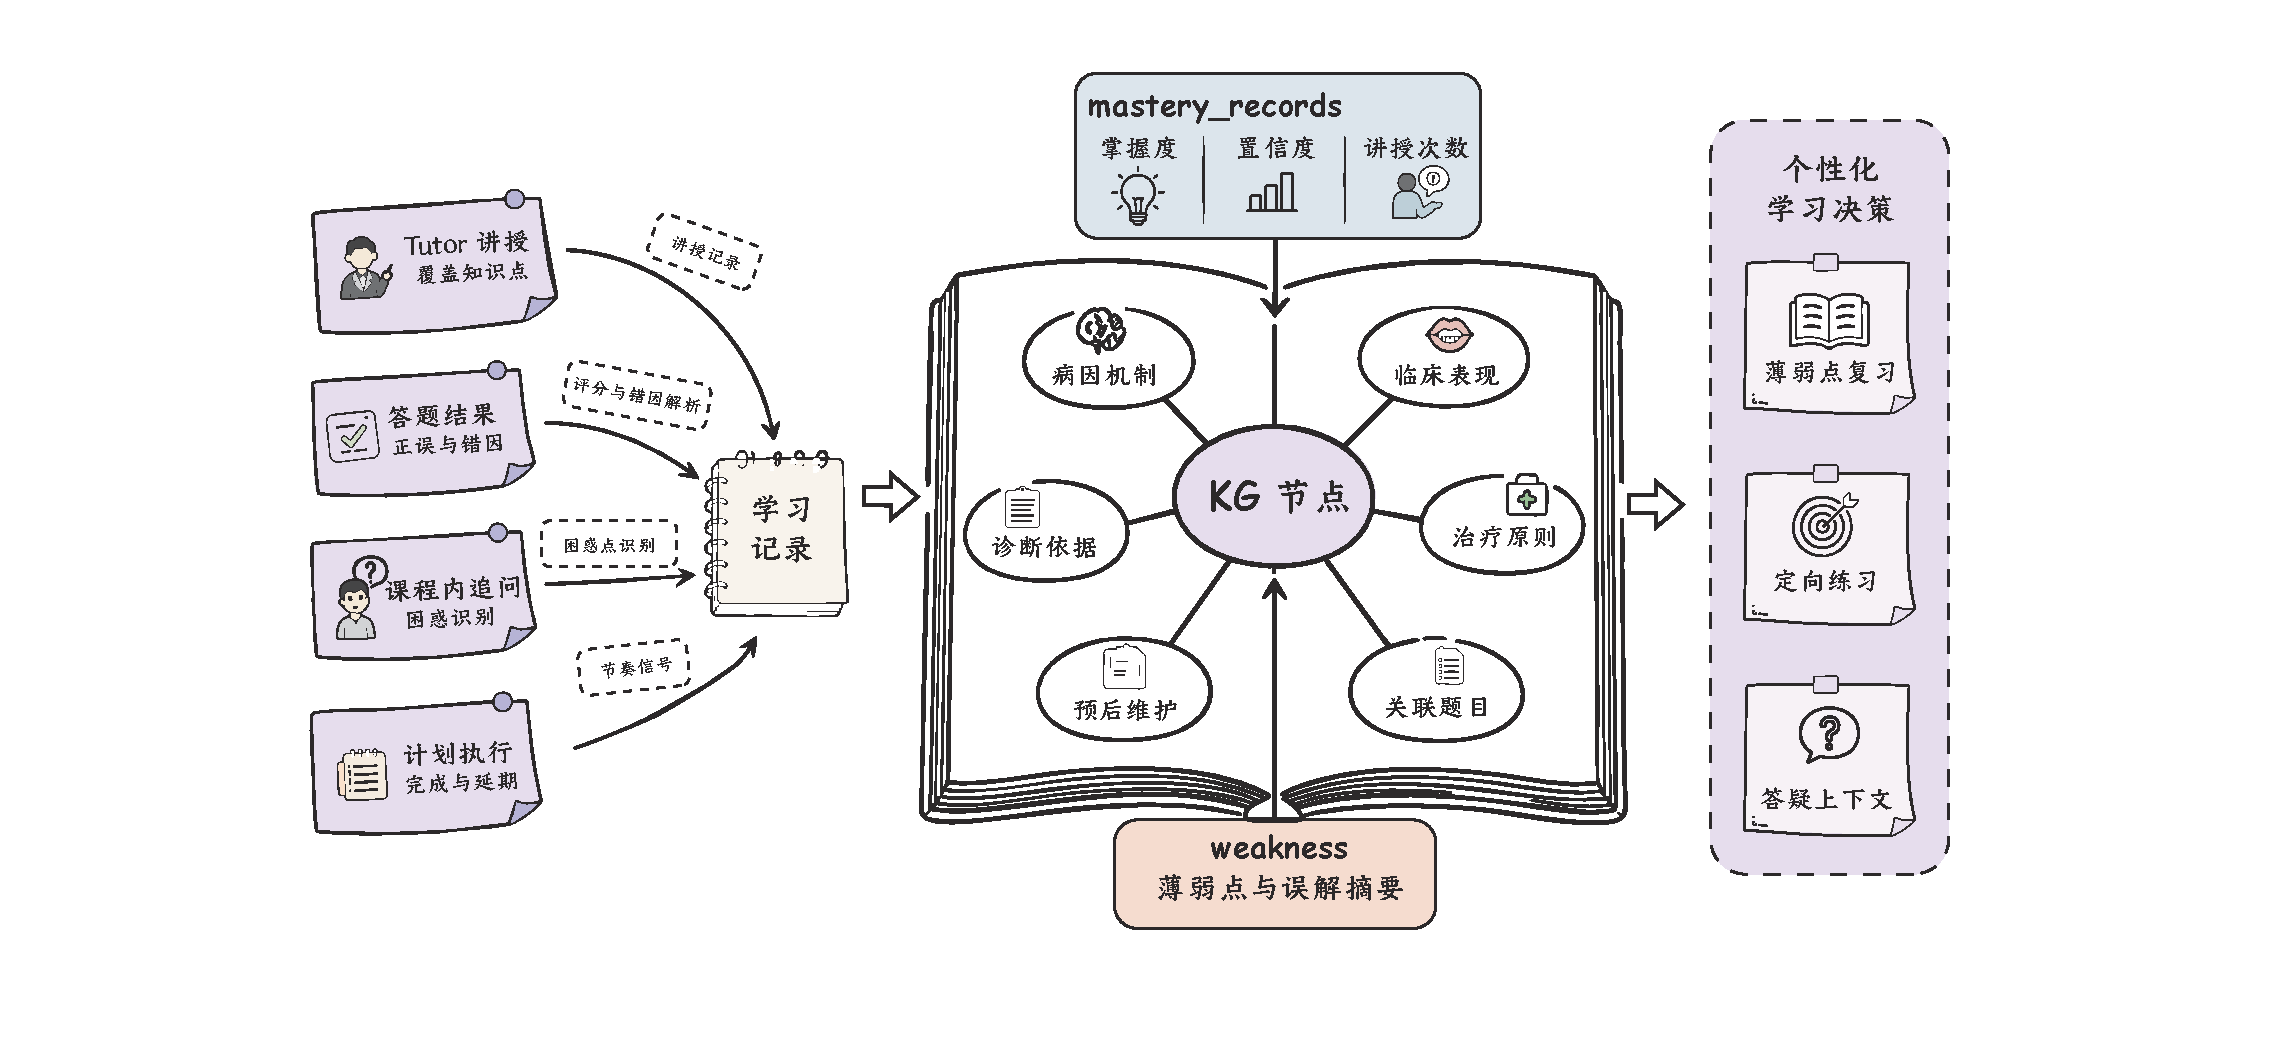
\includegraphics[width=0.94\linewidth]{figures/KG-knowledge-trace.pdf}
  \caption{学习行为与 KG 节点关联流程}
  \label{fig:learning-behavior-to-kg}
\end{figure}

如图\ref{fig:learning-behavior-to-kg}所示，知识图谱能够发挥课程组织和学习状态定位的双重作用，在为路径规划提供概念依赖与章节边界的同时，让薄弱点回顾、定向练习和答疑上下文能够聚焦到相关知识单元。相较于只记录总正确率的方式，节点级追踪能够进一步识别学习者对哪些具体知识内容掌握不足，更适合口腔医学中诊断条件、疾病分期、适应证与治疗原则容易发生混淆的学习任务。具体行为对后续学习状态的影响如表\ref{tab:learning-behavior-effects}所示。

\begin{table}[H]
  \centering
  \caption{主要学习行为对画像与知识状态的影响}
  \label{tab:learning-behavior-effects}
  \begin{tabularx}{\linewidth}{p{0.20\linewidth}p{0.34\linewidth}X}
    \toprule
    学习行为 & 主要记录内容 & 画像与状态更新 \\
    \midrule
    Tutor 讲授 & 小节、覆盖 KG 节点、讲授次数 & 写入 \texttt{tutor\_exposure}，形成小幅掌握度与置信度增量 \\
    答题正确 & 题目、关联节点、评分结果 & 提升对应节点的掌握度，并更新课程进度 \\
    答题错误 & 错选原因、误解摘要、关联节点、补救建议 & 降低相关节点掌握度，写入薄弱点和错因模式 \\
    课程内追问 & 问题、上下文、困惑节点、答疑结果 & 对明确困惑写入薄弱点与问答掌握记录，扩展性提问保留为交互记录 \\
    数字问诊 & 诊断结果、五域分数、遗漏要点、关联知识节点 & 更新掌握度、接触次数、置信度与薄弱点，并影响后续病例选择 \\
    计划完成或延期 & 任务状态、日期变化、完成情况 & 写入节奏类记忆，为后续任务密度和优先级调整提供输入 \\
    \bottomrule
  \end{tabularx}
\end{table}

\section{掌握学习反馈循环}

根据掌握学习理论指出的测评后的针对性反馈与补救机会能够帮助学习者逐步达成预设学习目标\cite{bloom1968mastery}的思想，OralSage 设计“测评、分析、反馈、再练习、再规划”的连续循环。Assessment 能够对学习者提交的错误答案，结合讲义小节和关联知识节点提供正确答案解释，生成错选原因，总结误解摘要，为学习者提供复习和知识补救建议。随后，相关知识节点的掌握状态和薄弱点记录进入学习画像，并供后续讲解、问答和计划推荐使用。

\begin{figure}[H]
  \centering
  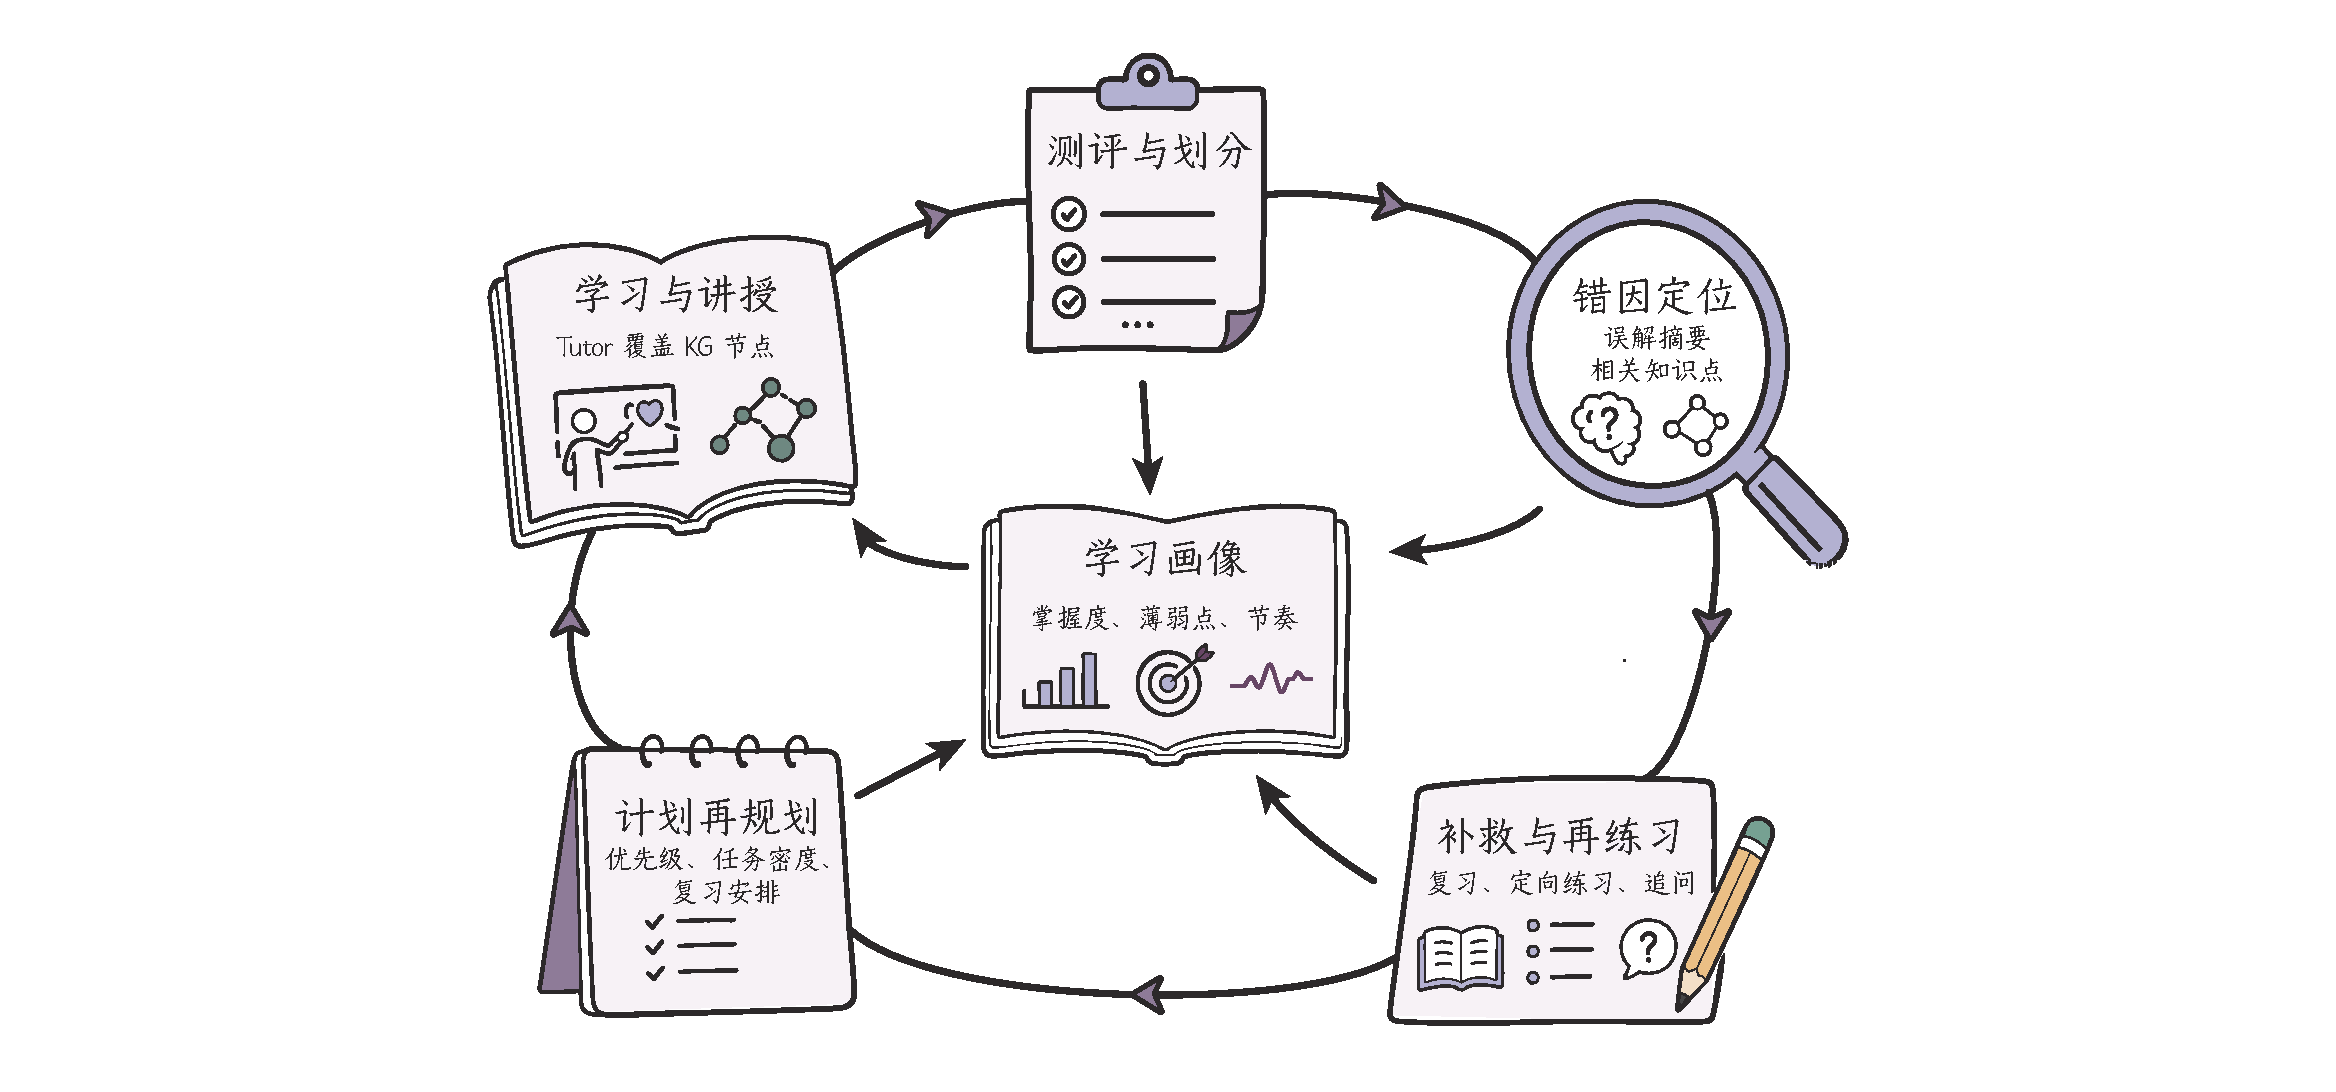
\includegraphics[width=0.94\linewidth]{figures/profile-feedback-loop.pdf}
  \caption{掌握学习反馈循环}
  \label{fig:mastery-feedback-loop}
\end{figure}

如图\ref{fig:mastery-feedback-loop}所示，反馈循环的重点在于将补救行动重新写入学习轨迹。学习者完成薄弱点复习、定向练习或阶段测评后，新的行为事件会进入 L1 层，经过摘要和长期记忆更新影响下一次学习决策。系统由此能够将一次答错转化为后续课程中的可执行任务，并持续组织相应的复习安排。

\section{画像可视化}

学习画像页将抽象的学习状态转化为学习者易于理解的可视化界面。页面展示近期学习天数、本日计划、完成记录、每日可用时间和学习活动趋势，并通过能力雷达图呈现自主规划、执行反馈、学习节奏、薄弱点修正、知识掌握和练习反馈等维度；当前学习风格、易错点与错因、目标导向、学习偏好及事件时间线也会在同一页面集中呈现。这些信息不仅用于展示学习结果，也帮助学习者理解近期完成了哪些任务、哪些知识仍需巩固，以及当前学习安排依据何种状态形成。

此外，用户可以重新完成测评来更新偏好基线，系统能够实时记录历史学习行为和知识状态。通过学习趋势、易错点和事件时间线，学习者可以回顾自身状态的变化；通过重新测评和学习计划入口，学习者也可以对原有偏好与后续安排进行调整。画像可视化由此不仅承担结果展示功能，也在系统的个性化判断与学习者的自主决策之间建立可理解、可回顾和可调整的交互界面。

% !TeX root = ../main.tex

\chapter{BKT/DKT 驱动的知识追踪与认知状态估计}
\label{sec:knowledge-tracing}

\section{技术定位与设计目标}

学习画像需要解决的核心问题，不只是记录学习者做过哪些题、问过哪些问题，而是推断学习者对每一个知识点是否已经形成稳定掌握。口腔医学知识具有强依赖、强迁移和高混淆度的特点，同一个错误答案可能源于概念边界不清、机制链条断裂、诊断条件遗漏或治疗适应证误判。若系统只使用答对加分、答错扣分的方式维护 \texttt{mastery\_by\_kg\_node}，则难以区分“真正掌握”“猜对”“会但失误”和“证据不足”四类状态，也无法表达系统对掌握度判断的置信程度。

OralSage 因此在学习画像层引入知识追踪（Knowledge Tracing）机制，将学习者画像从静态标签和规则评分升级为动态认知状态建模。系统以口腔医学知识图谱中的 KG 节点作为 skill 单元，以学习者答题序列、课程讲授、追问困惑和复习反馈作为观测证据，持续估计每个知识点的隐含掌握概率。该机制以 BKT（Bayesian Knowledge Tracing）作为可解释的概率推断核心，并结合 DKT（Deep Knowledge Tracing）建模长序列依赖和跨知识点迁移关系\cite{corbett1994knowledge,piech2015deep}。

该模块的目标包括三个方面。第一，将 \texttt{mastery\_score} 从简单行为分数升级为 $P(\mathrm{mastery}\mid\mathrm{evidence})$ 后验概率。第二，为每个 KG 节点输出掌握概率、不确定性、证据次数和最近观测，支撑学习画像、复习调度和数字孪生仿真。第三，将 BKT 的可解释性与 DKT 的序列建模能力结合，使系统既能展示贝叶斯公式推断过程，又能捕捉“答对 A 后 B 的掌握概率同步提升”等复杂学习迁移。

\section{面向 KG 节点的 Skill 建模}

OralSage 将口腔医学知识图谱中的每一个可学习节点视为一个 skill。设知识图谱节点集合为 $\mathcal{K}=\{k_1,k_2,\ldots,k_N\}$，学习者 $u$ 在时刻 $t$ 对节点 $k$ 的认知状态表示为
\begin{equation}
  \mathcal{Z}_{u,k,t}=
  \left(
  p_{u,k,t},
  c_{u,k,t},
  \sigma_{u,k,t},
  n_{u,k,t},
  a_{u,k,t}
  \right),
  \label{eq:kt-state}
\end{equation}
其中 $p_{u,k,t}$ 表示掌握概率，$c_{u,k,t}$ 表示模型置信度，$\sigma_{u,k,t}$ 表示不确定性，$n_{u,k,t}$ 表示累计观测证据数量，$a_{u,k,t}$ 表示最近一次观测动作或结果。

系统将题目、课程节点、讲义小节、QA 困惑和复习计划统一映射到 KG 节点，使不同学习行为能够在同一 skill 空间中汇合。对于一条答题观测事件
\begin{equation}
  o_t=(u,q_t,\mathbf{k}_t,y_t,s_t),
\end{equation}
其中 $q_t$ 为题目编号，$\mathbf{k}_t$ 为题目关联的 KG 节点集合，$y_t\in\{0,1\}$ 表示答题是否正确，$s_t$ 表示得分。若一道题关联多个 KG 节点，则系统对每一个 $k\in\mathbf{k}_t$ 独立更新 BKT 后验，同时将该观测写入序列模型输入，使节点级独立推断和序列级联合建模保持一致。

\begin{table}[H]
  \centering
  \caption{知识追踪模块的输入信号}
  \label{tab:kt-input-signals}
  \begin{tabularx}{\linewidth}{p{0.24\linewidth}p{0.33\linewidth}X}
    \toprule
    输入来源 & 主要字段 & 建模作用 \\
    \midrule
    Assessment & \texttt{is\_correct}、\texttt{score}、\texttt{kg\_node\_ids} & 将答题结果转化为 BKT 观测事件 \\
    题目结构 & 题干、选项、正确答案、关联 KG 节点 & 确定观测对应的 skill 单元 \\
    Tutor 讲授 & 课程节点、讲授覆盖 KG 节点、讲授次数 & 作为学习转移和曝光证据 \\
    QA 困惑 & \texttt{confusion\_kg\_node\_ids}、\texttt{should\_reinforce} & 识别失误、混淆和潜在薄弱节点 \\
    学习计划 & 复习完成、延期、任务类型、计划日期 & 校准复习后掌握变化和执行稳定性 \\
    \bottomrule
  \end{tabularx}
\end{table}

该设计使学习画像具备节点级可追踪性。系统不只知道学生在某次测评中得了多少分，还知道这次观测分别支持或削弱了哪些 KG 节点的掌握判断，并能够解释每个判断来自哪些题目、哪些课程和哪些追问证据。

\section{BKT 贝叶斯后验更新}

BKT 将学习者对某个 skill 的真实掌握状态视为隐变量 $L_t$，将答题对错视为可观测变量 $O_t$。对每个 KG 节点 $k$，系统维护四类核心参数：
\begin{itemize}
  \item $P(L_0)$：初始掌握概率，表示学习者在没有观测证据前掌握该知识点的先验概率；
  \item $P(T)$：学习转移概率，表示一次学习或练习后从未掌握转为掌握的概率；
  \item $P(G)$：猜测概率，表示未掌握但答对的概率；
  \item $P(S)$：失误概率，表示已掌握但答错的概率。
\end{itemize}

当学生答对时，系统根据贝叶斯公式计算已掌握状态的后验概率：
\begin{equation}
  P(L_t\mid Correct)=
  \frac{P(L_t)(1-P(S))}
  {P(L_t)(1-P(S))+(1-P(L_t))P(G)}.
  \label{eq:bkt-correct}
\end{equation}

当学生答错时，系统计算
\begin{equation}
  P(L_t\mid Incorrect)=
  \frac{P(L_t)P(S)}
  {P(L_t)P(S)+(1-P(L_t))(1-P(G))}.
  \label{eq:bkt-incorrect}
\end{equation}

完成观测更新后，系统再引入学习转移：
\begin{equation}
  P(L_{t+1})=
  P(L_t\mid O_t)+
  \left(1-P(L_t\mid O_t)\right)P(T).
  \label{eq:bkt-transition}
\end{equation}

对于复习间隔较长、遗忘风险较高的知识点，系统同时支持遗忘项：
\begin{equation}
  P(L_{t+1})=
  P(L_t\mid O_t)(1-P(F))+
  \left(1-P(L_t\mid O_t)\right)P(T),
  \label{eq:bkt-forget}
\end{equation}
其中 $P(F)$ 表示遗忘概率。通过式\eqref{eq:bkt-correct}--式\eqref{eq:bkt-forget}，系统能够区分“答对是因为掌握”与“答对可能只是猜测”，也能够区分“答错说明没学会”与“答错可能是失误”。这比单纯按照正确率更新掌握度更符合真实学习过程。

\begin{algorithm}[H]
  \caption{面向 KG 节点的 BKT 后验更新}
  \label{alg:bkt-kg-node}
  \begin{algorithmic}[1]
    \Require 学习者 $u$，题目 $q_t$，关联节点集合 $\mathbf{k}_t$，观测结果 $y_t$
    \Ensure 更新后的知识追踪状态集合 $\mathcal{Z}_{u,t+1}$
    \For{每一个 KG 节点 $k\in\mathbf{k}_t$}
      \State 读取节点 $k$ 的上一时刻掌握概率 $P(L_t)$ 与 BKT 参数
      \If{$y_t=1$}
        \State 根据式\eqref{eq:bkt-correct}计算答对后的掌握后验
      \Else
        \State 根据式\eqref{eq:bkt-incorrect}计算答错后的掌握后验
      \EndIf
      \State 根据式\eqref{eq:bkt-transition}和式\eqref{eq:bkt-forget}更新 $P(L_{t+1})$
      \State 计算不确定性、置信度、证据次数和观测追踪信息
      \State 写入 \texttt{knowledge\_tracing\_states}，并同步更新 \texttt{mastery\_by\_kg\_node}
    \EndFor
  \end{algorithmic}
\end{algorithm}

\section{不确定性估计与置信度表达}

知识追踪的价值不仅在于输出一个掌握概率，还在于表达系统对该判断是否有把握。OralSage 使用概率熵刻画认知状态不确定性。设某节点掌握概率为 $p$，则不确定性定义为
\begin{equation}
  U(p)=
  -\frac{p\log p+(1-p)\log(1-p)}{\log 2}.
  \label{eq:kt-uncertainty}
\end{equation}
当 $p$ 接近 $0.5$ 时，系统最不确定；当 $p$ 接近 $0$ 或 $1$ 时，系统判断更明确。该指标使画像能够展示“掌握概率较高但证据不足”“掌握概率中等且不确定性高”“掌握概率低且证据稳定”等不同状态。

模型置信度同时考虑证据数量和概率确定性：
\begin{equation}
  C_{u,k}=
  \lambda
  \left(1-e^{-n_{u,k}/\rho}\right)
  +(1-\lambda)(1-U(p_{u,k})),
  \label{eq:kt-confidence}
\end{equation}
其中 $n_{u,k}$ 为该节点累计观测次数，$\rho$ 控制证据增长速度，$\lambda$ 控制证据量与概率确定性的权重。该设计避免系统在单次答对后过度自信，也避免在多次稳定表现后仍然给出模糊判断。

\begin{table}[H]
  \centering
  \caption{知识追踪状态的结构化输出}
  \label{tab:kt-output-fields}
  \begin{tabularx}{\linewidth}{p{0.28\linewidth}p{0.27\linewidth}X}
    \toprule
    输出字段 & 含义 & 用途 \\
    \midrule
    \texttt{p\_mastery} & KG 节点掌握后验概率 & 作为画像掌握度、复习调度和路径仿真的核心输入 \\
    \texttt{uncertainty} & 掌握判断的不确定性 & 标记需要诊断题确认的知识点 \\
    \texttt{confidence} & 综合证据量和概率确定性的置信度 & 向学生解释系统判断是否可靠 \\
    \texttt{evidence\_count} & 节点累计观测次数 & 区分冷启动判断与稳定判断 \\
    \texttt{last\_observation\_correct} & 最近一次答题观测 & 展示最新学习反馈 \\
    \texttt{parameters} & BKT 参数集合 & 支持算法解释和参数校准 \\
    \texttt{trace} & 先验、后验、来源和模型信息 & 支持答辩展示、调试和审计 \\
    \bottomrule
  \end{tabularx}
\end{table}

前端画像页将该输出转化为“认知状态追踪”可视化：每个 KG 节点展示掌握概率条、不确定性标记、模型置信度、证据次数和最近观测。对于掌握概率低且不确定性高的节点，系统标记为“需要诊断”；对于掌握概率低且证据充分的节点，系统标记为“稳定薄弱”；对于掌握概率高但复习间隔较长的节点，系统交由 SM-2/FSRS 调度器判断复习窗口。

\section{DKT 深度序列建模}

BKT 在单个 skill 上具有清晰的概率解释，但口腔医学学习中还存在复杂的跨节点依赖。例如，学生在“牙周袋形成机制”上连续答对，往往意味着其对“附着丧失”“牙槽骨吸收进展”和“牙周炎分期”也具备更高的理解基础；学生在“根管治疗适应证”上反复错误，也可能影响其对“根尖周炎治疗原则”的后续表现。OralSage 因此采用 DKT 层对答题序列进行深度建模。

设学生的第 $t$ 次答题输入为
\begin{equation}
  \mathbf{x}_t=
  \operatorname{Embed}(k_t,y_t,s_t,\Delta t_t),
  \label{eq:dkt-input}
\end{equation}
其中 $k_t$ 为知识点编号，$y_t$ 为答题结果，$s_t$ 为得分，$\Delta t_t$ 为距上次学习或答题的时间间隔。序列编码器使用 LSTM 或 Transformer 对历史答题轨迹进行建模：
\begin{equation}
  \mathbf{h}_t=
  \operatorname{SeqEncoder}(\mathbf{x}_1,\mathbf{x}_2,\ldots,\mathbf{x}_t),
  \label{eq:dkt-hidden}
\end{equation}
并输出所有 KG 节点的下一次答对概率：
\begin{equation}
  \hat{\mathbf{y}}_{t+1}=
  \sigma(W\mathbf{h}_t+\mathbf{b}).
  \label{eq:dkt-output}
\end{equation}

其中 $\hat y_{t+1,k}$ 表示学习者下一次遇到节点 $k$ 相关题目时答对的概率。与 BKT 不同，DKT 不要求每个 skill 只受自身历史影响，而是通过序列隐状态捕捉跨节点迁移。系统将 DKT 输出与 BKT 后验进行融合：
\begin{equation}
  \bar p_{u,k,t}=
  \omega_k P_{\mathrm{BKT}}(L_{u,k,t})
  +(1-\omega_k)\hat y_{u,k,t}^{\mathrm{DKT}},
  \label{eq:bkt-dkt-fusion}
\end{equation}
其中 $\omega_k$ 由该节点证据数量、BKT 不确定性和序列模型置信度共同决定。证据较少或节点间迁移较强时，DKT 权重提高；证据充分且 BKT 后验稳定时，BKT 权重提高。该融合机制兼顾 BKT 的可解释性和 DKT 的表达能力。

\section{知识图谱约束的跨节点迁移}

为了使 DKT 输出符合口腔医学知识结构，系统在序列建模之外引入知识图谱约束。设 $A$ 为 KG 节点依赖矩阵，$A_{ij}$ 表示节点 $i$ 对节点 $j$ 的前置或关联强度，则跨节点掌握度传播定义为
\begin{equation}
  \tilde p_{u,j,t}=
  \bar p_{u,j,t}
  +
  \mu
  \sum_{i\in\operatorname{Pre}(j)}
  A_{ij}
  \left(\bar p_{u,i,t}-\bar p_{u,j,t}\right),
  \label{eq:kg-constrained-kt}
\end{equation}
其中 $\operatorname{Pre}(j)$ 表示节点 $j$ 的前置知识集合，$\mu$ 为图传播强度。该公式使系统能够根据前置知识状态校准后继节点预测。例如，若“牙周组织解剖基础”掌握概率较低，则系统会降低对“牙周袋形成机制”和“牙槽骨吸收进展”的高阶掌握预测；若前置节点稳定掌握，则系统能够更合理地解释后续节点掌握概率提升。

知识图谱约束还用于避免深度模型产生不符合课程结构的迁移。例如，若两个 KG 节点在图谱中没有明确依赖、共现或同章关系，则 DKT 的跨节点影响会被图约束削弱；若节点之间存在“前置”“组成”“鉴别”“治疗依据”等关系，则迁移权重相应增强。由此，知识追踪结果既具备序列模型的学习能力，又保持专业知识结构上的可解释性。

\section{与学习画像、复习调度和数字孪生的协同}

知识追踪模块位于 OralSage 个性化学习闭环的认知状态估计层。Assessment 产生答题观测，Knowledge Tracing 计算 KG 节点掌握后验，Memory/User Model 将后验写入长期学习画像，SM-2/FSRS Scheduler 根据掌握概率和遗忘风险生成复习窗口，Student Twin Agent 再基于这些状态模拟不同学习路径的收益。

该协同链路可以表示为
\[
\begin{aligned}
&\text{Assessment/QA/Tutor}
\rightarrow
\text{Knowledge Tracing}
\rightarrow
\text{Memory/User Model}
\\
&\rightarrow
\text{SM-2/FSRS Scheduler}
\rightarrow
\text{Student Twin}
\rightarrow
\text{Study Plan}.
\end{aligned}
\]

在画像层，\texttt{mastery\_by\_kg\_node} 保存的不再是单纯的累计分数，而是包含 \texttt{score}、\texttt{confidence}、\texttt{uncertainty}、\texttt{evidence\_count} 和 \texttt{model} 的认知状态摘要。在复习层，SM-2/FSRS 使用掌握后验和不确定性判断哪些节点需要复习、哪些节点需要诊断题确认。在数字孪生层，Student Twin 使用知识追踪状态估计学习路径收益，将“继续新课”“薄弱点复习”“复习后小测”等策略建立在更稳定的认知状态之上。

\begin{table}[H]
  \centering
  \caption{知识追踪与下游模块的协同关系}
  \label{tab:kt-downstream}
  \begin{tabularx}{\linewidth}{p{0.22\linewidth}p{0.34\linewidth}X}
    \toprule
    下游模块 & 使用的知识追踪输出 & 技术作用 \\
    \midrule
    学习画像 & 掌握概率、置信度、不确定性、证据次数 & 将画像升级为动态认知状态模型 \\
    SM-2/FSRS & 掌握概率、证据次数、最近观测、遗忘风险 & 计算复习优先级和最佳复习窗口 \\
    Student Twin & 瓶颈节点、掌握概率、不确定性 & 模拟不同学习路径下的风险下降和掌握提升 \\
    Study Plan & 低掌握节点、高不确定节点、复习债务 & 生成 \texttt{review\_section}、诊断题和小测任务 \\
    前端可视化 & 概率条、置信度、不确定性、观测轨迹 & 向学生解释系统为什么推荐某个知识点 \\
    \bottomrule
  \end{tabularx}
\end{table}

\section{工程落地与接口结构}

系统使用 \texttt{knowledge\_tracing\_states} 维护每个用户、每个 KG 节点的认知状态。该状态表采用用户编号和 KG 节点编号作为联合主键，保存 skill 名称、掌握概率、不确定性、置信度、证据次数、正确次数、错误次数、最近观测、BKT 参数和推断 trace。该结构既能支持 BKT 的实时更新，也能承载 DKT 序列模型输出，使上层模块始终读取统一认知状态。

\begin{table}[H]
  \centering
  \caption{知识追踪状态表的核心字段}
  \label{tab:kt-state-table}
  \begin{tabularx}{\linewidth}{p{0.30\linewidth}p{0.25\linewidth}X}
    \toprule
    字段 & 类型含义 & 技术作用 \\
    \midrule
    \texttt{user\_id}、\texttt{kg\_node\_id} & 学生与 skill 标识 & 定位节点级认知状态 \\
    \texttt{p\_mastery} & 掌握后验概率 & 替代简单累计掌握分数 \\
    \texttt{uncertainty} & 概率熵归一化结果 & 表达模型不确定性 \\
    \texttt{confidence} & 综合置信度 & 支持解释与前端展示 \\
    \texttt{evidence\_count} & 观测次数 & 判断证据是否充分 \\
    \texttt{correct\_count}、\texttt{incorrect\_count} & 正误统计 & 支持校准和评估 \\
    \texttt{parameters\_json} & BKT 参数 & 保存 skill 级模型参数 \\
    \texttt{trace\_json} & 推断过程 & 保存先验、后验、来源和模型信息 \\
    \bottomrule
  \end{tabularx}
\end{table}

系统提供 \texttt{/api/learning/knowledge-tracing/\{user\_id\}} 接口返回学习者的知识追踪状态。接口输出包含 \texttt{schema\_version}、\texttt{model} 和 \texttt{states}，其中每个 state 对应一个 KG 节点。该接口使前端能够直接展示认知状态，也使答辩演示能够呈现系统如何从一次答题观测更新出新的掌握概率。

\section{评估指标与展示方式}

知识追踪模块从预测准确性、概率校准、认知解释和学习收益四个层面进行评估。预测准确性关注模型对下一次答题正确率的预测能力；概率校准关注掌握概率与真实正确率是否一致；认知解释关注系统能否清楚说明掌握判断来自哪些证据；学习收益关注基于知识追踪的复习计划是否提升后续表现。

\begin{table}[H]
  \centering
  \caption{BKT/DKT 知识追踪模块评估指标}
  \label{tab:kt-evaluation}
  \begin{tabularx}{\linewidth}{p{0.25\linewidth}p{0.30\linewidth}X}
    \toprule
    指标类别 & 指标名称 & 含义 \\
    \midrule
    预测准确性 & Next Question AUC & 使用当前认知状态预测下一题是否答对 \\
    概率校准 & Calibration Error & 比较 $P(\mathrm{mastery})$ 与真实正确率的一致性 \\
    状态稳定性 & Posterior Stability & 多次观测后掌握概率是否趋于稳定 \\
    不确定性质量 & Uncertainty Reduction & 证据增加后不确定性是否合理下降 \\
    学习收益 & Mastery Uplift & 知识追踪驱动复习后的掌握度提升 \\
    计划效果 & Review Hit Rate & 被模型标记为低掌握节点的复习命中率 \\
    \bottomrule
  \end{tabularx}
\end{table}

在答辩展示中，系统可以选择一个口腔医学知识点展示完整推断过程：初始掌握概率为 $P(L_0)$，学生答对后根据猜测概率和失误概率计算后验，再经过学习转移得到新的 $P(L_{t+1})$；若学生随后答错，系统不会简单扣固定分，而是根据 slip 与 guess 参数重新解释该观测。前端同时展示掌握概率曲线、不确定性变化和证据次数，使评委能够直观看到系统如何把答题行为转化为动态认知状态。

通过 BKT/DKT 知识追踪，OralSage 将学习画像从“记录型画像”提升为“推断型画像”。系统不再只保存学生做过什么，而是持续估计学生脑中对每个 KG 节点的隐含掌握状态，并将这一状态用于复习调度、数字孪生仿真和个性化计划生成，从而形成具有教育 AI 技术深度的认知建模闭环。

% !TeX root = ../main.tex

\chapter{认知科学驱动的间隔重复复习调度}
\label{sec:spaced-repetition-scheduling}

\section{技术定位与设计目标}

口腔医学学习不仅要求学生理解单个概念，还要求其在较长周期内稳定保持对疾病机制、诊断依据、鉴别诊断、治疗原则和临床决策链条的记忆。传统学习计划通常依据固定规则安排复习，例如“答错后次日复习”或“章节结束后统一回顾”。这类学习计划虽然能够简单地覆盖一些明显的模式，但没有显式刻画记忆随时间衰减的过程，也难以回答“某一个具体知识点在今天是否已经到达最佳复习窗口”这一问题。

OralSage 在学习计划模块中进一步引入认知科学驱动的间隔重复调度思想，将复习安排从经验规则提升为面向知识点的记忆状态建模。系统不再仅根据任务完成状态或错误记录静态生成计划，而是读取学习画像中的 \texttt{weak\_kg\_node\_ids}、\texttt{mastery\_by\_kg\_node}、课程掌握记录和直接问答掌握记录，为每一个薄弱 KG 节点计算下一次复习时间、记忆保持率估计和复习优先级，并输出为 \texttt{review\_section} 类型的学习计划项。

该模块的核心目标包括三个方面。第一，建立面向 KG 节点的记忆单元，使复习对象从“章节”细化到“具体知识点”。第二，引入 SM-2 与 FSRS 两类间隔重复算法框架，使计划推荐具备可解释的数学依据。第三，将复习调度结果写入学习计划，使 Planner、Assessment、QA 和 Memory/User Model 之间形成可闭环的复习决策链路。

\section{基于 SM-2 的确定性复习调度}

SM-2 是经典间隔重复算法之一，其主要思想是根据学习者每次回忆质量更新重复次数、难度因子和下次复习间隔\cite{wozniak1990sm2}。OralSage 将该算法从传统卡片级复习扩展为 KG 节点级复习，使口腔医学知识图谱中的每一个概念节点都可以拥有独立的复习状态。

\subsection{知识点记忆状态建模}

设第 $k$ 个知识点的记忆状态为
\begin{equation}
  \mathcal{M}_k=(m_k,c_k,d_k,n_k,EF_k,I_k,t_k),
\end{equation}
其中 $m_k$ 表示掌握度，$c_k$ 表示置信度，$d_k$ 表示知识点难度，$n_k$ 表示连续成功复习次数，$EF_k$ 表示易度因子，$I_k$ 表示当前复习间隔，$t_k$ 表示上次学习或复习时间。与普通背词软件不同，OralSage 的状态不是由用户手动维护，而是由多源学习证据自动融合得到。

\begin{table}[H]
  \centering
  \caption{间隔重复调度器的输入信号}
  \label{tab:spaced-review-inputs}
  \begin{tabularx}{\linewidth}{p{0.26\linewidth}p{0.27\linewidth}X}
    \toprule
    输入来源 & 主要字段 & 技术作用 \\
    \midrule
    长期学习记忆 & \texttt{weaknesses}、\texttt{mastery} & 抽取薄弱知识点、错误理解和低掌握度节点 \\
    学习画像 & \texttt{mastery\_by\_kg\_node} & 提供跨课程的节点级掌握状态 \\
    课程掌握记录 & \texttt{mastery\_records} & 记录课程学习、讲授覆盖和题目表现后的掌握度变化 \\
    直接问答记录 & \texttt{direct\_qa\_mastery\_records} & 捕捉学生主动提问暴露出的困惑节点 \\
    学习计划记录 & \texttt{study\_plan\_items} & 避免重复推荐，并为后续执行反馈提供闭环入口 \\
    \bottomrule
  \end{tabularx}
\end{table}

在候选知识点合并阶段，系统按照 KG 节点编号进行聚合，保留最小掌握度、最高薄弱严重度、最近一次学习时间、证据来源和关联课程信息。该设计使同一知识点即使来自课程学习、直接问答和错题反馈等不同路径，也能被统一映射到同一个复习调度单元。

\subsection{掌握度到回忆质量的映射}

传统 SM-2 依赖用户在复习后给出 $0$ 到 $5$ 的回忆质量评分。面向智能学习系统时，OralSage 使用学习画像中的掌握度自动估计回忆质量。设 $m_k\in[0,1]$ 为知识点掌握度，$b_k$ 表示该节点是否为薄弱点，则质量分数 $q_k$ 定义为
\begin{equation}
  q_k =
  \begin{cases}
  2, & \tilde m_k < 0.35,\\
  3, & 0.35 \le \tilde m_k < 0.55,\\
  4, & 0.55 \le \tilde m_k < 0.78,\\
  5, & \tilde m_k \ge 0.78,
  \end{cases}
  \quad
  \tilde m_k =
  \begin{cases}
  m_k-0.08, & b_k=1,\\
  m_k, & b_k=0.
  \end{cases}
  \label{eq:sm2-quality-mapping}
\end{equation}

该映射保留了 SM-2 对回忆质量的离散判断，同时引入薄弱点惩罚项，使系统在识别到“概念混淆”“机制链条不完整”“诊断依据遗漏”等风险时，更倾向于缩短复习间隔。对于口腔医学中容易混淆的知识，例如牙龈炎与牙周炎鉴别、牙髓炎与根尖周炎鉴别、牙周袋深度与附着丧失关系，该设计能够比单纯正确率更敏感地捕捉复习需求。

\subsection{SM-2 状态更新公式}

设知识点当前易度因子为 $EF_k$，复习质量为 $q_k$，则 SM-2 的易度因子更新为
\begin{equation}
  EF'_k = \max\left(1.3,\ EF_k + 0.1 - (5-q_k)\left(0.08+(5-q_k)0.02\right)\right).
  \label{eq:sm2-ef}
\end{equation}

若 $q_k<3$，说明本次回忆失败，系统将连续成功次数重置为 $0$，并将复习间隔设为 $1$ 天。若 $q_k\ge3$，则进入成功复习分支：
\begin{equation}
  I'_k =
  \begin{cases}
  1, & n'_k=1,\\
  6, & n'_k=2,\\
  \operatorname{round}(I_k EF'_k), & n'_k>2.
  \end{cases}
  \label{eq:sm2-interval}
\end{equation}

为避免稀疏学习记录导致过长间隔，系统对 $I'_k$ 设置上界，并将其与知识点难度、掌握度和证据置信度共同用于优先级排序，而不是机械地只按到期日期排序。

\section{遗忘曲线与复习优先级函数}

SM-2 给出了下次复习间隔，但学习计划推荐还需要在多个候选知识点之间排序。OralSage 因此进一步构建遗忘曲线估计与优先级函数，将“是否到期”“薄弱程度”“知识点难度”和“距上次学习时间”统一纳入调度。

设 $\Delta t_k$ 为当前日期与上次学习日期之间的间隔，$S_k$ 为知识稳定度估计，则知识点 $k$ 的记忆保持率估计为
\begin{equation}
  \hat R_k = \exp\left(-\frac{\Delta t_k}{S_k}\right),
  \quad
  S_k = I'_k(0.85+0.3c_k).
  \label{eq:retention-estimate}
\end{equation}

其中，$c_k$ 为证据置信度。掌握证据越稳定，系统越允许间隔略微延长；置信度较低或薄弱证据较强时，系统会更保守地安排复习。对于计划推荐排序，OralSage 使用如下优先级函数：
\begin{equation}
  P_k=\operatorname{clip}\left(
  0.28+
  \frac{(1-m_k)\cdot O_k\cdot H_k\cdot B_k}{2.8},
  0,\ 0.98
  \right),
  \label{eq:review-priority}
\end{equation}
其中
\begin{equation}
  O_k=1+\min\left(2,\frac{\max(0,\ t_{\mathrm{now}}-(t_k+I'_k))}{\max(1,I'_k)}\right),
  \quad
  H_k=0.85+0.65d_k,
  \quad
  B_k =
  \begin{cases}
  1.18, & k\in \mathcal{W},\\
  1.00, & k\notin \mathcal{W}.
  \end{cases}
\end{equation}

$O_k$ 表示逾期因子，$H_k$ 表示难度因子，$B_k$ 表示薄弱点权重。该公式使推荐排序不只关注“错没错”，而是同时考虑“掌握得是否牢固”“是否已经越过最佳复习窗口”“知识点本身是否困难”和“是否被多源证据识别为薄弱点”。因此，系统能够将学习计划推荐从规则触发升级为可解释的算法调度。

\begin{algorithm}[H]
  \caption{面向 KG 节点的 SM-2 复习调度}
  \label{alg:kg-sm2-review}
  \begin{algorithmic}[1]
    \Require 学习者编号 $u$，目标日期 $T$，长期记忆 $L$，课程掌握记录 $C$
    \Ensure 排序后的复习候选集合 $\mathcal{R}$
    \State 从 $L$ 和 $C$ 中抽取薄弱节点、低掌握节点和问答困惑节点
    \State 按 KG 节点编号聚合同一知识点的掌握度、置信度、难度和证据来源
    \For{每一个候选知识点 $k$}
      \State 根据式\eqref{eq:sm2-quality-mapping}计算回忆质量 $q_k$
      \State 根据式\eqref{eq:sm2-ef}和式\eqref{eq:sm2-interval}更新 $EF'_k$ 与 $I'_k$
      \State 根据式\eqref{eq:retention-estimate}估计保持率 $\hat R_k$
      \State 根据式\eqref{eq:review-priority}计算复习优先级 $P_k$
      \State 生成包含 \texttt{kg\_node\_ids} 与 \texttt{spaced\_repetition} 追踪信息的候选项
    \EndFor
    \State 按 $P_k$、复习到期日期和知识点名称排序，输出前若干项
  \end{algorithmic}
\end{algorithm}

\section{面向 FSRS 的高级记忆状态扩展}

SM-2 的优点是计算稳定、解释直接、对数据量要求低。为了进一步提升长期个性化能力，OralSage 同时预留 FSRS（Free Spaced Repetition Scheduler）扩展方向。FSRS 使用 DSR 记忆模型，将每个记忆单元表示为 Difficulty、Stability 和 Retrievability 三个核心变量\cite{openfsrs2025algorithm}，比 SM-2 更适合在积累大量复习日志后进行参数学习和个体化拟合。

\subsection{DSR 记忆模型}

在 FSRS 框架下，知识点 $k$ 的记忆状态可表示为
\begin{equation}
  \mathcal{F}_k=(D_k,S_k,R_k),
\end{equation}
其中 $D_k$ 表示知识点对该学习者的主观难度，$S_k$ 表示记忆稳定度，$R_k$ 表示在当前时刻成功回忆该知识点的概率。其遗忘曲线可写为
\begin{equation}
  R_k(t,S_k)=\left(1+\mathrm{FACTOR}\cdot\frac{t}{S_k}\right)^{\mathrm{DECAY}},
  \label{eq:fsrs-forgetting}
\end{equation}
其中 $t$ 为距上次复习的时间。FSRS 通过设置 \texttt{DECAY} 与 \texttt{FACTOR}，使 $t=S_k$ 时保持率接近目标阈值，例如 $R=0.9$。当系统设定期望保持率为 $\rho$ 时，可以反推出下一次复习间隔：
\begin{equation}
  I_{\rho,k}=
  \frac{S_k}{\mathrm{FACTOR}}
  \left(\rho^{1/\mathrm{DECAY}}-1\right).
  \label{eq:fsrs-interval}
\end{equation}

与 SM-2 相比，FSRS 不再只使用连续成功次数和易度因子控制间隔，而是显式估计“知识点难度”和“记忆稳定度”。这使系统能够区分两类不同情况：一类是学生暂时答错但长期稳定度较高的知识点，另一类是学生偶尔答对但稳定度很低的知识点。后者在口腔医学学习中更危险，因为其表面正确率可能掩盖对诊断边界、机制推理或治疗适应证的不稳定理解。

\subsection{从系统日志学习 FSRS 参数}

FSRS 的高级性在于其参数可以由学习者历史复习记录反向拟合。设一次复习日志为
\begin{equation}
  x_i=(k_i,t_i,g_i,y_i),
\end{equation}
其中 $k_i$ 为知识点，$t_i$ 为距上次复习时间，$g_i$ 为系统或学习者给出的回忆等级，$y_i\in\{0,1\}$ 表示是否成功回忆。系统可以使用历史日志最小化预测回忆概率与真实表现之间的交叉熵：
\begin{equation}
  \mathcal{L}(\theta)=
  -\sum_i
  \left[
  y_i\log R_{\theta}(t_i,S_{k_i})
  +(1-y_i)\log(1-R_{\theta}(t_i,S_{k_i}))
  \right].
  \label{eq:fsrs-loss}
\end{equation}

在 OralSage 中，FSRS 参数学习可以直接利用现有的学习事件表、掌握度记录、直接问答记录和学习计划完成记录。随着学生完成更多 \texttt{review\_section} 任务，系统能够从真实复习正确率、任务延迟情况和答题结果中学习个体化参数，使复习调度从“基于通用遗忘曲线的估计”逐步升级为“基于个人记忆曲线的预测”。

\begin{table}[H]
  \centering
  \caption{SM-2 与 FSRS 在 OralSage 中的技术分工}
  \label{tab:sm2-fsrs-comparison}
  \begin{tabularx}{\linewidth}{p{0.18\linewidth}X X}
    \toprule
    维度 & SM-2 调度器 & FSRS 扩展调度器 \\
    \midrule
    状态变量 & 重复次数、易度因子、复习间隔 & 难度、稳定度、可回忆概率 \\
    数据需求 & 少量掌握度和薄弱点记录即可运行 & 需要持续积累复习日志和正确率反馈 \\
    可解释性 & 公式简单，适合展示单次调度过程 & 可展示个体遗忘曲线与目标保持率 \\
    个性化程度 & 基于掌握度和薄弱证据进行轻量个性化 & 可通过历史日志训练学习者级或群体级参数 \\
    工程角色 & 当前确定性落地方案，稳定生成 \texttt{review\_section} & 后续高级优化方向，用于自适应记忆预测和工作量模拟 \\
    \bottomrule
  \end{tabularx}
\end{table}

\section{与多智能体学习闭环的协同}

间隔重复调度是 OralSage 多智能体学习闭环中的一个算法决策层。Tutor 在讲授过程中记录知识点覆盖和学习进度，QA 根据学生追问识别困惑节点，Assessment 根据答题结果生成错误原因和补救建议，Memory/User Model 将上述证据写入长期学习画像，Study-Planner 再根据 SM-2 或 FSRS 调度结果生成复习任务。

该闭环可以表示为
\[
\text{Tutor/QA/Assessment}
\rightarrow
\text{Memory/User Model}
\rightarrow
\text{SM-2/FSRS Scheduler}
\rightarrow
\text{Study Plan}
\rightarrow
\text{Review Feedback}.
\]

在学习计划输出层，调度器将候选知识点转换为结构化计划项：
\begin{itemize}
  \item \texttt{task\_type}: 设为 \texttt{review\_section}，表示该任务是面向知识点的复习区块；
  \item \texttt{kg\_node\_ids}: 保存需要复习的 KG 节点，支持后续定位讲义、题目和证据片段；
  \item \texttt{learning\_scope}: 保存调度算法、掌握度、难度、易度因子、间隔天数、下次复习日期和保持率估计；
  \item \texttt{priority}: 保存由掌握度、逾期因子、难度因子和薄弱点权重共同计算得到的复习优先级。
\end{itemize}

这种结构化输出使复习计划具备可追溯性，系统不仅推荐了某个复习任务，还可以解释推荐的数学依据：该知识点掌握度较低，距上次学习已经超过模型计算出的最佳复习间隔，记忆保持率估计下降，因此被提升到今日计划中。

\section{评估指标与展示方式}

OralSage 从算法准确性、学习效果和计划执行三个层面构建评估指标。算法层面关注保持率预测与实际复习正确率之间的偏差；学习效果层面关注薄弱知识点在复习后的掌握度提升；执行层面关注推荐任务是否被学生完成，以及逾期复习债务是否下降。

\begin{table}[H]
  \centering
  \caption{间隔重复调度模块的评估指标}
  \label{tab:spaced-review-evaluation}
  \begin{tabularx}{\linewidth}{p{0.24\linewidth}p{0.32\linewidth}X}
    \toprule
    指标类别 & 指标名称 & 含义 \\
    \midrule
    预测准确性 & Retention Calibration & 比较模型估计保持率与实际复习正确率是否一致 \\
    学习收益 & Mastery Uplift & 统计复习前后相关 KG 节点掌握度提升幅度 \\
    计划质量 & Review Debt Reduction & 统计逾期复习节点数量和逾期天数是否下降 \\
    执行行为 & Completion Rate & 统计 \texttt{review\_section} 任务完成比例 \\
    算法对比 & SM-2/FSRS A/B Test & 比较不同调度策略下的正确率、完成率和任务负担 \\
    \bottomrule
  \end{tabularx}
\end{table}

当曲线下降到目标保持率阈值附近时，系统生成复习任务；当学生完成复习并答对相关题目后，稳定度提升，下一次复习间隔随之延长。通过对比不同算法策略下的保持率、掌握度提升和复习落后进度变化，系统评估了 SM-2 与 FSRS 在口腔医学学习场景中的适用性和效果。


% !TeX root = ../main.tex

\chapter{学习数字孪生学生 Agent}
\label{sec:student-twin-simulation}

\section{技术定位与设计目标}

在传统个性化学习系统中，学习计划通常根据当前薄弱点、已完成任务和用户设定的学习时间进行推荐。这类推荐能够回答“今天可以学什么”，但难以进一步回答“如果选择不同学习路径，学生未来的掌握度会如何变化”“当前 20 分钟应该优先投入到哪个知识点收益最大”“某个薄弱点是否会阻塞后续章节理解”等更高阶问题。OralSage 因此在学习画像和间隔重复调度之上进一步设计\textbf{学习数字孪生学生 Agent}，为每个真实学习者构建一个可计算、可更新、可仿真的虚拟学习分身。

数字孪生的核心思想是为现实对象建立动态映射模型，使系统能够在虚拟空间中观察状态、预测变化并评估不同决策方案\cite{grieves2017digitaltwin}。面向口腔医学学习场景，OralSage 将这一思想转化为学习过程仿真：系统根据学习者历史答题、追问行为、学习节奏、薄弱 KG 节点、掌握度和复习债务构建 Student Twin，再在虚拟学生状态上模拟多条候选学习路径，预测每条路径带来的掌握度增益、风险下降和认知负荷变化，最终向学习计划模块输出可执行任务。

该模块的设计目标包括四个方面。第一，将学习画像从“状态记录”升级为“状态预测”，使系统不仅知道学生当前哪里薄弱，还能预测后续可能在哪里卡住。第二，将学习计划推荐从单点排序升级为反事实路径仿真，使系统能够比较“继续新课”“先复习薄弱点”“复习后小测”等不同策略的预期收益。第三，将知识图谱、SM-2/FSRS 复习调度和掌握度追踪统一到同一个仿真状态中，使推荐结果具有明确的算法解释。第四，为前端提供可视化证据，使学生能够看到虚拟分身的风险、瓶颈和推荐路径，而不是只接收一个静态任务列表。

\section{虚拟学生状态建模}

学习数字孪生首先需要将多源学习证据压缩为可计算的学生状态。设学习者 $u$ 在日期 $T$ 的虚拟状态为
\begin{equation}
  \mathcal{S}_{u,T}=
  \left(
  \mathbf{m}_{u,T},
  \mathbf{r}_{u,T},
  \mathbf{d}_{u,T},
  \mathbf{b}_{u,T},
  \tau_{u,T},
  \pi_u
  \right),
  \label{eq:student-twin-state}
\end{equation}
其中 $\mathbf{m}_{u,T}$ 表示 KG 节点掌握度向量，$\mathbf{r}_{u,T}$ 表示记忆保持率估计，$\mathbf{d}_{u,T}$ 表示知识点难度向量，$\mathbf{b}_{u,T}$ 表示薄弱点与错因证据，$\tau_{u,T}$ 表示可用学习时间和执行节奏，$\pi_u$ 表示学习偏好与讲解风格。

与一次性问卷画像不同，Student Twin 的状态由系统内已有学习证据持续生成。课程讲授记录提供知识点覆盖情况，Assessment 记录答题正确率和错因，QA 记录学生主动暴露的困惑点，Memory/User Model 聚合长期薄弱点和掌握度，间隔重复调度器提供遗忘风险和复习债务。各类输入信号如表\ref{tab:student-twin-inputs}所示。

\begin{table}[H]
  \centering
  \caption{Student Twin 的输入信号与建模作用}
  \label{tab:student-twin-inputs}
  \begin{tabularx}{\linewidth}{p{0.24\linewidth}p{0.32\linewidth}X}
    \toprule
    输入来源 & 主要字段 & 建模作用 \\
    \midrule
    学习画像 & \texttt{mastery\_by\_kg\_node}、每日可用时间、学习偏好 & 构建节点级掌握度、学习节奏和策略约束 \\
    长期学习记忆 & \texttt{weaknesses}、错因摘要、近期学习事件 & 识别稳定薄弱点和容易阻塞后续学习的概念断点 \\
    间隔重复调度 & \texttt{retention\_estimate}、\texttt{overdue\_days}、\texttt{priority} & 提供遗忘曲线风险、复习债务和最佳复习窗口 \\
    课程与测评记录 & 课程覆盖、题目结果、掌握度增量 & 估计学习行为对知识状态的影响 \\
    计划执行记录 & 完成、延期、跳过和打卡行为 & 估计执行稳定性与任务负荷承受能力 \\
    \bottomrule
  \end{tabularx}
\end{table}

当前工程落地版本采用确定性、可解释的状态构建方式：系统优先读取 SM-2 调度器返回的薄弱节点和复习候选项，将掌握度、保持率、逾期天数和难度转化为瓶颈风险；若复习候选不足，则回退读取长期记忆中的薄弱点和画像中的低掌握度 KG 节点，保证 Student Twin 在冷启动阶段仍能生成可用仿真结果。后续高级版本可进一步接入深度知识追踪模型，将历史答题序列编码为隐状态，预测每个 KG 节点的未来答题成功概率\cite{corbett1994knowledge,piech2015deep}。

\section{瓶颈风险识别与遗忘风险融合}

在口腔医学学习中，真正影响后续学习的往往不是单个题目的得失，而是某些前置概念未被稳定掌握。例如牙龈炎与牙周炎边界、牙周袋形成机制、牙槽骨吸收进展、牙髓炎与根尖周炎鉴别等知识点，一旦掌握不稳，会在病例分析、诊断选择和治疗方案理解中反复造成错误。Student Twin 因此将薄弱点建模为具有风险分数的瓶颈节点。

设知识点 $k$ 的掌握度为 $m_k$，保持率估计为 $R_k$，逾期复习天数为 $o_k$，难度为 $d_k$，则瓶颈风险定义为
\begin{equation}
  B_k=\operatorname{clip}
  \left(
  \alpha(1-m_k)+\beta(1-R_k)+\gamma \min(1,o_k/5)+\eta d_k,
  0,1
  \right).
  \label{eq:student-twin-bottleneck-risk}
\end{equation}

其中 $\alpha,\beta,\gamma,\eta$ 分别控制掌握不足、记忆衰减、复习逾期和知识难度的影响。当前落地版本使用轻量启发式权重，使结果具有稳定可解释性；在数据规模扩大后，该权重可以通过复习正确率、错题复发率和计划完成记录自动拟合。对于每个瓶颈节点，系统同时保存证据来源、推荐原因和调度轨迹，使前端能够展示“为什么该知识点被判定为风险点”。

学生整体风险由排名靠前的瓶颈节点聚合得到：
\begin{equation}
  \operatorname{Risk}(u,T)=
  \frac{1}{|\mathcal{K}_{top}|}
  \sum_{k\in \mathcal{K}_{top}}B_k,
  \label{eq:student-twin-overall-risk}
\end{equation}
其中 $\mathcal{K}_{top}$ 为风险最高的若干 KG 节点。该设计避免大量低风险知识点稀释真正关键的瓶颈，使系统更关注“最可能让学生卡住的少数知识点”。

\section{反事实学习路径仿真}

Student Twin 的核心创新不只是识别薄弱点，而是在虚拟学生状态上模拟不同学习路径的结果。给定当前状态 $\mathcal{S}_{u,T}$ 和候选学习动作集合 $\mathcal{A}$，系统构建状态转移函数：
\begin{equation}
  \mathcal{S}_{u,T+1}^{(a)}=
  f_{\theta}(\mathcal{S}_{u,T},a),
  \quad a\in\mathcal{A}.
  \label{eq:student-twin-transition}
\end{equation}

候选动作可以包括继续学习新章节、优先复习最高风险薄弱点、复习后进行小测、先做病例题再回看讲义、降低任务量只完成核心回顾等。系统在不真正改变用户数据的情况下，预测每种动作对掌握度、风险和认知负荷的影响，并进行反事实比较。当前版本内置三类基础策略：

\begin{itemize}
  \item \textbf{继续学习新章节}：适用于整体风险较低、复习债务较少的学习者，收益来自课程推进，但对薄弱点修复有限；
  \item \textbf{薄弱点间隔复习}：优先处理 SM-2/FSRS 判定接近或超过复习窗口的知识点，主要目标是降低遗忘风险；
  \item \textbf{薄弱点复习 + 小测}：先修复最高风险节点，再通过病例题或基础练习验证迁移效果，适合风险较高但仍有一定可用时间的场景。
\end{itemize}

对每条路径 $a$，系统估计掌握度增益 $\Delta M_a$、风险下降 $\Delta R_a$、认知负荷 $C_a$ 和时间适配惩罚 $P_a$，并使用收益函数进行排序：
\begin{equation}
  J(a)=
  \lambda_1\Delta M_a+
  \lambda_2\Delta R_a-
  \lambda_3C_a-
  \lambda_4P_a.
  \label{eq:student-twin-path-score}
\end{equation}

当前工程版本采用可解释的线性打分函数：
\[
  J(a)=2.2\Delta M_a+1.8\Delta R_a-C_a-P_a.
\]
该函数体现了系统的教学策略：在短时学习场景中，降低关键薄弱点风险通常比机械推进新课更重要；当学习者可用时间较少时，系统会降低高负荷路径的优先级。后续可扩展为模型预测控制（Model Predictive Control）形式，在未来多天计划窗口内滚动优化：
\begin{equation}
  \max_{a_1,\ldots,a_H}
  \sum_{h=1}^{H}
  \delta^{h-1}
  J(a_h)
  \quad
  \text{s.t.}\quad
  \sum_{h=1}^{H}t(a_h)\le T_{\mathrm{budget}}.
  \label{eq:student-twin-mpc}
\end{equation}

通过这种方式，学习计划不再只是对当天任务排序，而可以扩展为对未来一周甚至一个复习周期的滚动仿真优化。

\begin{algorithm}[H]
  \caption{Student Twin 反事实路径仿真}
  \label{alg:student-twin-simulation}
  \begin{algorithmic}[1]
    \Require 学习者编号 $u$，计划日期 $T$，可用时间 $\tau$，学习画像 $P$，长期记忆 $M$
    \Ensure 推荐路径 $a^\ast$ 与可写入学习计划的任务集合 $\mathcal{I}$
    \State 从 $P$ 与 $M$ 中读取 KG 掌握度、薄弱点、学习偏好和执行节奏
    \State 调用 SM-2/FSRS 调度器生成候选复习节点与遗忘风险
    \State 将掌握度、保持率、逾期天数和难度融合为瓶颈风险 $B_k$
    \State 构造虚拟学生状态 $\mathcal{S}_{u,T}$
    \State 生成候选路径集合 $\mathcal{A}$，包括新课、复习、复习后小测等策略
    \For{每条候选路径 $a\in\mathcal{A}$}
      \State 估计路径后的掌握度增益 $\Delta M_a$ 与风险下降 $\Delta R_a$
      \State 估计认知负荷 $C_a$ 和时间适配惩罚 $P_a$
      \State 根据式\eqref{eq:student-twin-path-score}计算路径得分 $J(a)$
    \EndFor
    \State 选择 $a^\ast=\arg\max_{a\in\mathcal{A}}J(a)$
    \State 将 $a^\ast$ 的步骤转化为 \texttt{student\_twin} 类学习计划项
    \State 输出瓶颈节点、路径比较、反事实解释和推荐任务
  \end{algorithmic}
\end{algorithm}

\section{当前工程落地形态}

OralSage 已将 Student Twin 作为独立学习智能体接入后端和前端。后端提供面向用户编号的数字孪生查询接口 \url{/api/learning/student-twin/{user_id}}，返回 \texttt{StudentTwinAgent} 的结构化仿真结果，包括整体掌握度、整体风险、记忆保持率、复习债务、瓶颈节点、候选路径、推荐路径、推荐计划项和反事实解释。系统能力接口中同步暴露 \texttt{learning\_student\_twin}，便于前端和演示环境识别该创新模块。

接口输出遵循 \texttt{student\_twin.simulation.v1} 结构，核心字段如表\ref{tab:student-twin-output}所示。

\begin{table}[H]
  \centering
  \caption{Student Twin API 的核心输出结构}
  \label{tab:student-twin-output}
  \begin{tabularx}{\linewidth}{p{0.25\linewidth}p{0.27\linewidth}X}
    \toprule
    输出字段 & 数据含义 & 前端或计划模块用途 \\
    \midrule
    \texttt{state} & 掌握度、风险、保持率、复习债务 & 展示虚拟学生当前状态与风险水平 \\
    \texttt{bottlenecks} & 风险最高的 KG 节点列表 & 展示可能卡住的概念、原因和证据来源 \\
    \texttt{paths} & 多条候选学习路径及仿真分数 & 支持比较不同学习策略的预期收益 \\
    \texttt{recommended\_path\_id} & 系统推荐路径编号 & 标记最优路径并驱动默认计划生成 \\
    \texttt{recommended\_plan\_items} & 可写入计划的任务项 & 将仿真结果落地为 \texttt{review\_section} 或练习任务 \\
    \texttt{counterfactual} & 反事实解释文本 & 向用户解释为什么不选择另一条路径 \\
    \texttt{trace} & 模型、公式和生成时间 & 便于答辩展示与系统调试 \\
    \bottomrule
  \end{tabularx}
\end{table}

前端学习计划页新增数字孪生卡片，集中展示虚拟学生状态、关键瓶颈、候选路径和一键生成计划操作。如图\ref{fig:student-twin-ui-mockup}所示，页面通过指标卡展示整体掌握度、卡点风险、保持率和复习债务，通过瓶颈列表显示薄弱 KG 节点，通过路径比较呈现“继续新课”“间隔复习”“复习 + 小测”等策略的预期提升。学生可以直接将推荐路径转换为今日学习计划，使仿真结果进入真实任务执行闭环。

\begin{figure}[H]
  \centering
  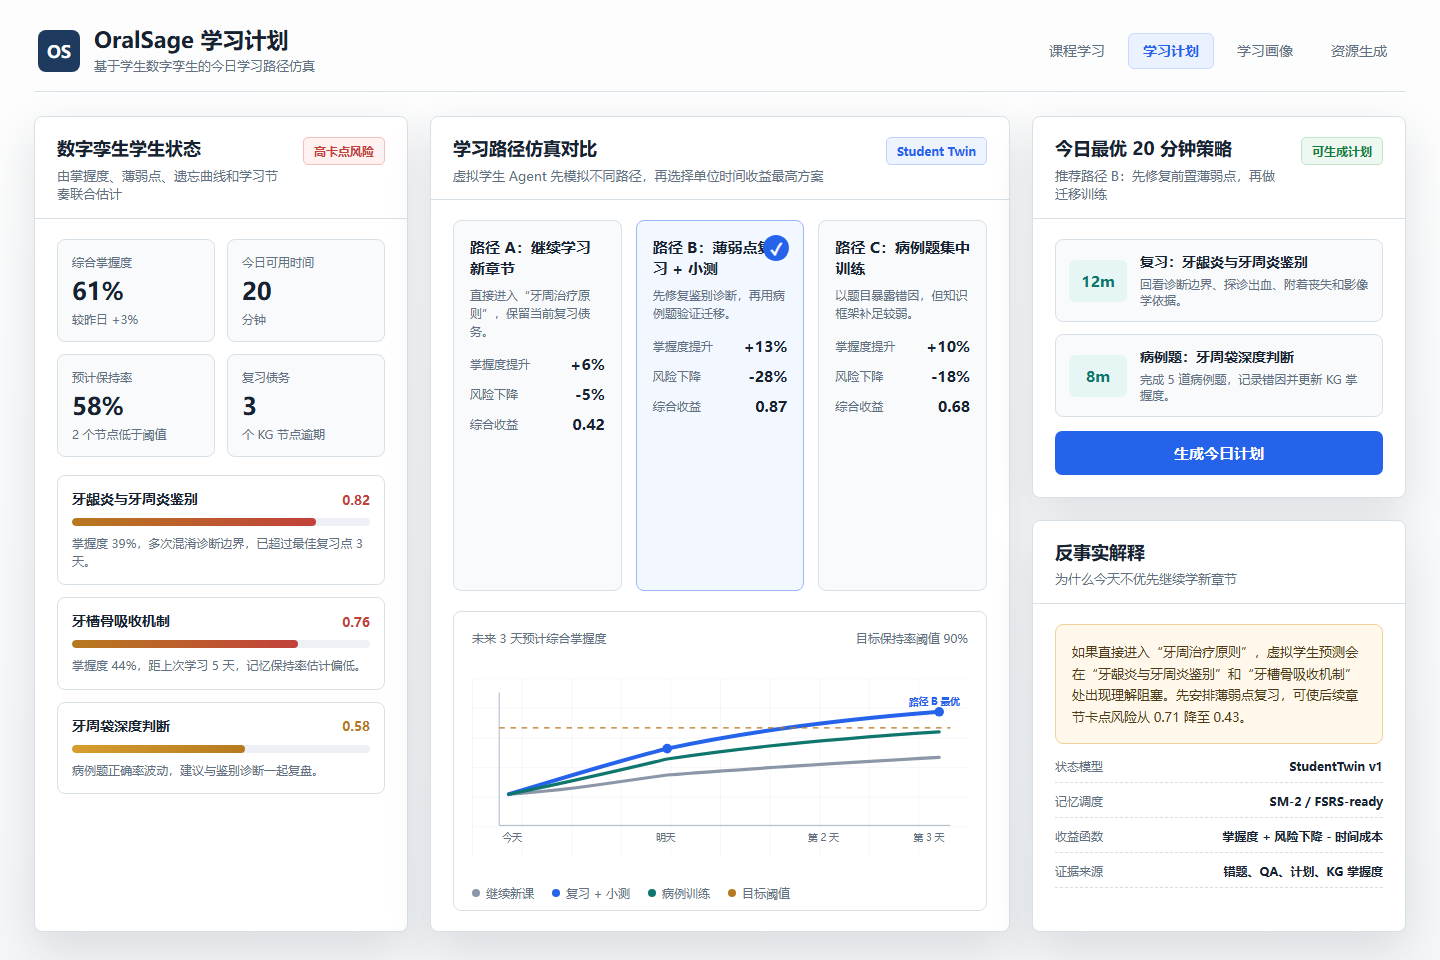
\includegraphics[width=0.96\linewidth]{student-twin-ui-mockup.png}
  \caption{学习数字孪生 Agent 的前端可视化示意}
  \label{fig:student-twin-ui-mockup}
\end{figure}

从工程实现角度看，当前版本选择确定性仿真而非黑盒深度模型，主要原因在于参赛展示阶段需要稳定复现、便于解释和易于与现有学习计划模块集成。该版本已经实现了“画像读取--瓶颈识别--路径仿真--推荐任务--计划写入”的最小闭环；在数据积累后，可以平滑替换状态估计器和转移函数，而不改变前端交互和计划接口。

\section{与多智能体系统的协同关系}

Student Twin 并不是孤立的推荐模块，而是 OralSage 多智能体学习闭环中的预测层。Planner 负责生成课程结构，Tutor 负责讲授，QA 捕捉用户追问，Assessment 诊断答题结果，Memory/User Model 更新长期状态，SM-2/FSRS Scheduler 估计复习窗口，Student Twin 则在这些状态之上进行未来路径仿真。

其协同链路可以表示为
\[
\begin{aligned}
&\text{Tutor/QA/Assessment}
\rightarrow
\text{Memory/User Model}
\rightarrow
\text{SM-2/FSRS Scheduler}
\\
&\rightarrow
\text{Student Twin}
\rightarrow
\text{Study Plan}.
\end{aligned}
\]

在该链路中，Student Twin 的角色是将已有状态转化为“如果这样学会怎样”的预测结果。它既可以服务于学习计划，也可以反向影响 Tutor 和 Assessment。例如，当 Student Twin 预测某个薄弱点会阻塞后续课程时，Tutor 可以在讲解新课前插入前置概念回顾；当仿真显示复习后仍存在较高风险时，Assessment 可以生成更聚焦的病例题；当计划执行多次延期时，Planner 可以降低任务密度并改为短时高收益路径。

\begin{table}[H]
  \centering
  \caption{Student Twin 与其他智能体的协同分工}
  \label{tab:student-twin-agent-collaboration}
  \begin{tabularx}{\linewidth}{p{0.22\linewidth}p{0.34\linewidth}X}
    \toprule
    协同对象 & 输入或输出关系 & 技术价值 \\
    \midrule
    Planner & 接收仿真推荐路径，调整学习顺序和任务密度 & 将课程规划从静态大纲转为预测驱动路径 \\
    Tutor & 根据瓶颈节点插入前置概念讲解 & 减少学生在后续章节中反复卡住 \\
    QA & 将高频追问转化为数字孪生的风险证据 & 让主动提问成为状态预测信号 \\
    Assessment & 根据仿真风险生成定向练习和病例题 & 用测评验证虚拟学生预测是否准确 \\
    Memory/User Model & 回收真实执行结果，更新孪生状态 & 形成仿真、执行、校准的闭环 \\
    Study Plan & 接收 \texttt{student\_twin} 类计划项 & 将路径仿真落地为可执行任务 \\
    \bottomrule
  \end{tabularx}
\end{table}

\section{高级扩展：概率孪生与策略优化}

当前实现是可解释的最小落地版本，已经能够支持答辩演示和产品闭环。为了进一步体现技术深度，Student Twin 可扩展为概率化、可学习、可优化的高级智能体。

\subsection{概率知识状态与不确定性估计}

现有掌握度可以从单一分数扩展为概率分布：
\begin{equation}
  m_k\sim \operatorname{Beta}(\alpha_k,\beta_k),
  \label{eq:student-twin-beta-mastery}
\end{equation}
其中 $\alpha_k$ 和 $\beta_k$ 分别由正确作答、错误作答、追问困惑和课程覆盖证据更新。这样系统不仅知道某个知识点掌握度约为 $0.6$，还知道该估计是否可靠。当样本较少或证据冲突时，Student Twin 可以输出较高不确定性，并推荐低成本诊断题而不是直接安排较长复习任务。

进一步地，系统可以将深度知识追踪或贝叶斯知识追踪作为状态估计器，使用学习事件序列预测未来答题成功概率。对于口腔医学中前后依赖强的知识结构，还可以引入知识图谱传播项，使某个前置节点的薄弱风险影响其后继节点：
\begin{equation}
  \tilde B_j =
  B_j+
  \mu
  \sum_{i\in \operatorname{Pre}(j)}
  w_{ij}B_i,
  \label{eq:student-twin-graph-risk}
\end{equation}
其中 $\operatorname{Pre}(j)$ 表示节点 $j$ 的前置知识集合，$w_{ij}$ 表示依赖强度。该扩展能够更准确地预测“下一章可能在哪里卡住”，而不仅是识别当前已经暴露的薄弱点。

\subsection{蒙特卡洛路径仿真}

当前版本对每条路径输出一个确定性收益分数。高级版本可以采用蒙特卡洛仿真，从掌握度分布、完成概率和遗忘曲线中采样，得到路径收益的置信区间：
\begin{equation}
  \hat J(a)=
  \frac{1}{N}
  \sum_{n=1}^{N}
  J^{(n)}(a),
  \quad
  \operatorname{Var}(J(a))=
  \frac{1}{N-1}
  \sum_{n=1}^{N}
  \left(J^{(n)}(a)-\hat J(a)\right)^2.
  \label{eq:student-twin-monte-carlo}
\end{equation}

前端可进一步展示“预计提升区间”和“策略风险区间”，例如某条路径虽然平均收益较高，但不确定性较大；另一条路径平均收益略低，但结果更稳定。这样，学习计划推荐可以从单一最优选择升级为风险感知决策。

\subsection{FSRS 记忆参数与数字孪生融合}

FSRS 的 Difficulty、Stability 和 Retrievability 变量可以直接作为 Student Twin 的记忆状态子空间。对于每个 KG 节点 $k$，系统可维护
\[
  \mathcal{F}_k=(D_k,S_k,R_k),
\]
并将其并入虚拟学生状态。完成一次 \texttt{review\_section} 后，系统根据复习正确率、作答时间和自信度更新 $D_k$ 与 $S_k$，再由 $R_k$ 预测下次复习时的回忆概率。与 SM-2 相比，FSRS 更适合在长期日志积累后学习个体化遗忘曲线，因此可以作为 Student Twin 的长期记忆动力学模型。

该扩展使答辩展示能够从“今天推荐什么任务”进一步升级为“系统如何拟合学生自己的遗忘曲线，并用该曲线模拟未来路径”。前端可展示不同学习路径下未来 7 天或 14 天的预计保持率曲线、掌握度曲线和复习债务变化曲线，从而体现算法性和高级感。

\subsection{强化学习式策略优化}

当系统积累足够多的计划执行和学习效果数据后，可以将学习路径选择建模为马尔可夫决策过程：
\begin{equation}
  \mathcal{M}=(\mathcal{S},\mathcal{A},P,R,\gamma),
\end{equation}
其中状态 $\mathcal{S}$ 为 Student Twin 的虚拟学生状态，动作 $\mathcal{A}$ 为不同学习策略，转移概率 $P$ 表示学习行为后的状态变化，奖励 $R$ 综合掌握度提升、风险下降、完成率和认知负荷。系统可以先使用离线日志进行策略评估，再在安全约束下进行轻量在线优化。由于教育场景需要稳定和可解释，实际产品中可采用“规则策略 + 学习型重排序”的混合方式，将强化学习限制在候选路径排序层，避免直接生成不可控任务。

\section{评估指标与答辩展示方式}

Student Twin 的评估应同时关注预测准确性、学习收益和用户执行效果。预测准确性衡量系统判断的瓶颈是否真的在后续答题或提问中出现；学习收益衡量推荐路径是否提升掌握度并降低错题复发；执行效果衡量数字孪生推荐是否更容易被学生完成。

\begin{table}[H]
  \centering
  \caption{学习数字孪生 Agent 的评估指标}
  \label{tab:student-twin-evaluation}
  \begin{tabularx}{\linewidth}{p{0.25\linewidth}p{0.32\linewidth}X}
    \toprule
    指标类别 & 指标名称 & 含义 \\
    \midrule
    预测准确性 & Bottleneck Hit Rate & 被预测为瓶颈的 KG 节点是否在后续错题、追问或低掌握记录中出现 \\
    风险校准 & Risk Calibration & 瓶颈风险分数与真实错误率、追问率之间的一致性 \\
    学习收益 & Simulated Uplift vs. Actual Uplift & 仿真预测的掌握度提升与真实掌握度变化是否接近 \\
    路径质量 & Counterfactual Gain & 推荐路径相对备选路径带来的风险下降差值 \\
    执行效果 & Completion Rate & 数字孪生生成计划项的完成率和延期率 \\
    负荷控制 & Cognitive Load Stability & 推荐任务是否在可用时间内完成，是否造成计划堆积 \\
    \bottomrule
  \end{tabularx}
\end{table}

在答辩展示中，可以选择同一名学生的学习画像作为输入，展示三层结果。第一层展示虚拟学生状态，包括掌握度、风险、保持率和复习债务；第二层展示系统预测的卡点知识点及证据来源；第三层展示多条学习路径的反事实比较，例如“继续新课预计风险下降 4\%”“先复习薄弱点预计风险下降 18\%”“复习后小测预计风险下降 24\%”。最后将推荐路径一键写入学习计划，形成“预测--仿真--决策--执行”的完整闭环。

由此，Student Twin 将 OralSage 的个性化能力从资源生成和任务推荐进一步推进到学习过程仿真层面。系统不只是根据已有规则推荐学习内容，而是为每个学生构建一个能够被观察、被模拟、被校准的虚拟学习分身，使口腔医学学习计划具备更强的技术可解释性、算法深度和创新展示价值。

% !TeX root = ../main.tex

\chapter{个性化学习资源生成}
\label{sec:resource-generation}

\definecolor{chfiveaccent}{HTML}{E9E9F5}

\section{设计思想}

第五章说明学习画像如何形成和更新，本章进一步说明这些个体信息如何转化为学习路径、学习计划、讲义、讲解和练习等可直接使用的学习资源。

口腔医学的学习困难往往来自知识体系庞大、前后依赖紧密，以及基础理论与临床判断之间存在较长的理解距离。面对同一主题，备考学习者更关心高频考点和诊断辨析，临床应用导向的学习者需要理解病例线索与治疗原则，刚接触课程的学习者则需要更充分的概念铺垫。统一的资源顺序和解释密度难以同时满足这些需求。

针对这一痛点，OralSage 采用学习画像驱动的资源生成流程，综合学习目标、基础水平、解释偏好、每日可用时间、学习节奏、知识掌握状态和薄弱内容，形成适合当前学习者的主题路径，再围绕路径生成讲义、互动讲解、语音、课件、知识结构图和练习。资源的个性化体现在学习什么、先学习什么、解释到何种深度、以何种节奏复习，以及何时进入练习和回顾。

这一设计将生成式人工智能置于明确的医学教育活动之中。近期研究指出，生成式人工智能能够支持医学教育中的内容组织和个体化辅导，教学目标、学习活动和专业判断决定了其实际价值\cite{lie2024harnessing,rodman2024using}。OralSage 围绕口腔医学主题建立连续学习过程，使资源生成服务于理解、应用、巩固和反馈四类学习活动。

\begin{figure}[H]
  \centering
  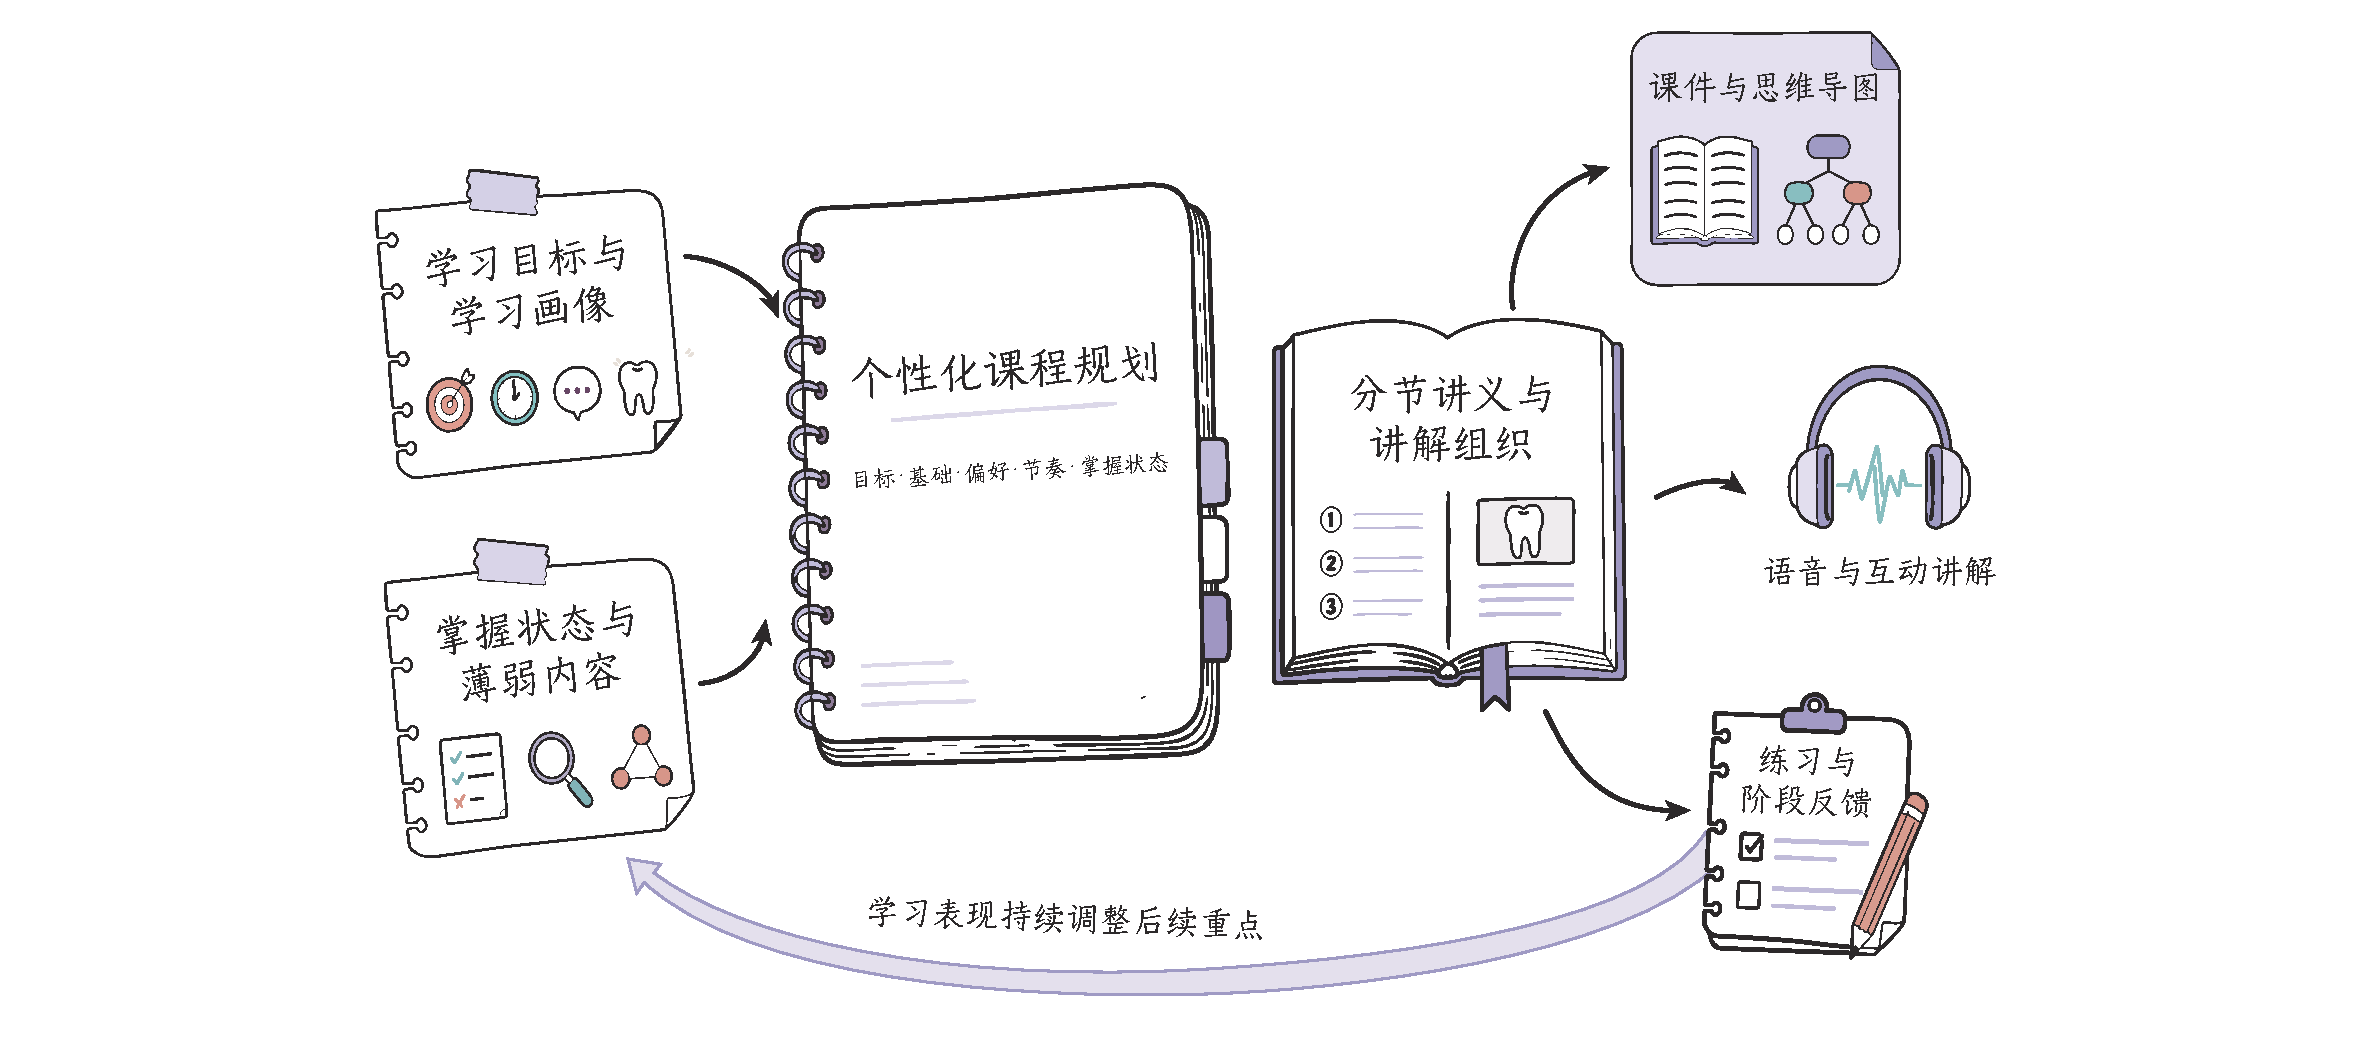
\includegraphics[width=\linewidth]{profile-resource-generation.pdf}
  \caption{学习画像驱动的个性化资源生成过程}
  \label{fig:personalized-resource-generation}
\end{figure}

如图\ref{fig:personalized-resource-generation}所示，学习者画像和知识状态共同决定课程规划。分节讲义承担课程内容的组织作用，互动讲解、语音、课件、知识结构图和练习围绕已规划的学习单元展开。练习表现和学习过程中的困惑进一步更新知识状态，为后续课程资源调整提供依据。

\begin{table}[H]
  \centering
  \caption{学习画像信息对资源生成的影响}
  \label{tab:profile-resource-mapping}
  \begin{tabularx}{\linewidth}{p{0.24\linewidth}p{0.30\linewidth}X}
    \toprule
    个性化信息 & 资源调节方向 & 学习效果 \\
    \midrule
    学习目标 & 调整课程范围、考点比重和案例比重 & 使学习内容贴近备考、课程学习或临床理解需求 \\
    基础水平与掌握状态 & 安排基础铺垫、机制展开和回顾内容 & 避免学习难度脱离当前理解基础 \\
    解释偏好 & 调整概念、病例、问题和考点的进入顺序 & 提升知识进入方式与个人习惯的匹配度 \\
    每日可用时间与节奏 & 调整小节长度、学习顺序和复习密度 & 使学习任务更适合持续完成 \\
    薄弱内容与错因 & 插入定向讲解、辨析和练习 & 将学习时间聚焦于真正需要巩固的内容 \\
    \bottomrule
  \end{tabularx}
\end{table}

\section{个性化学习路径与计划}

\subsection{知识状态感知的课程路径生成}

学习路径将学习画像中的目标、时间预算、知识状态和口腔医学知识图谱转化为可执行的学习单元序列。得到学习指令后，系统首先根据主题和知识图谱确定知识范围及其依赖关系，再结合学习目标、薄弱点、掌握度和学习节奏调整单元顺序与内容重点，最后为每个单元配置相应的讲义、讲解、练习与复习任务。由此，知识结构决定课程的基本边界，学习者的个人状态进一步决定实际学习路径。

在不同的情境下，系统会灵活采取不同的措施，生成节奏匹配的个性化资源。学习者提出备考学习的需求时，系统会优先呈现高频考点、薄弱内容回顾和阶段练习；重点在临床应用时，系统则倾向于由病例情境进入，再逐步讲授诊断依据与治疗原则；学习者需要查缺补漏时，低掌握度内容会获得更高优先级，并在相关学习单元后安排定向练习。

\begin{figure}[H]
  \centering
  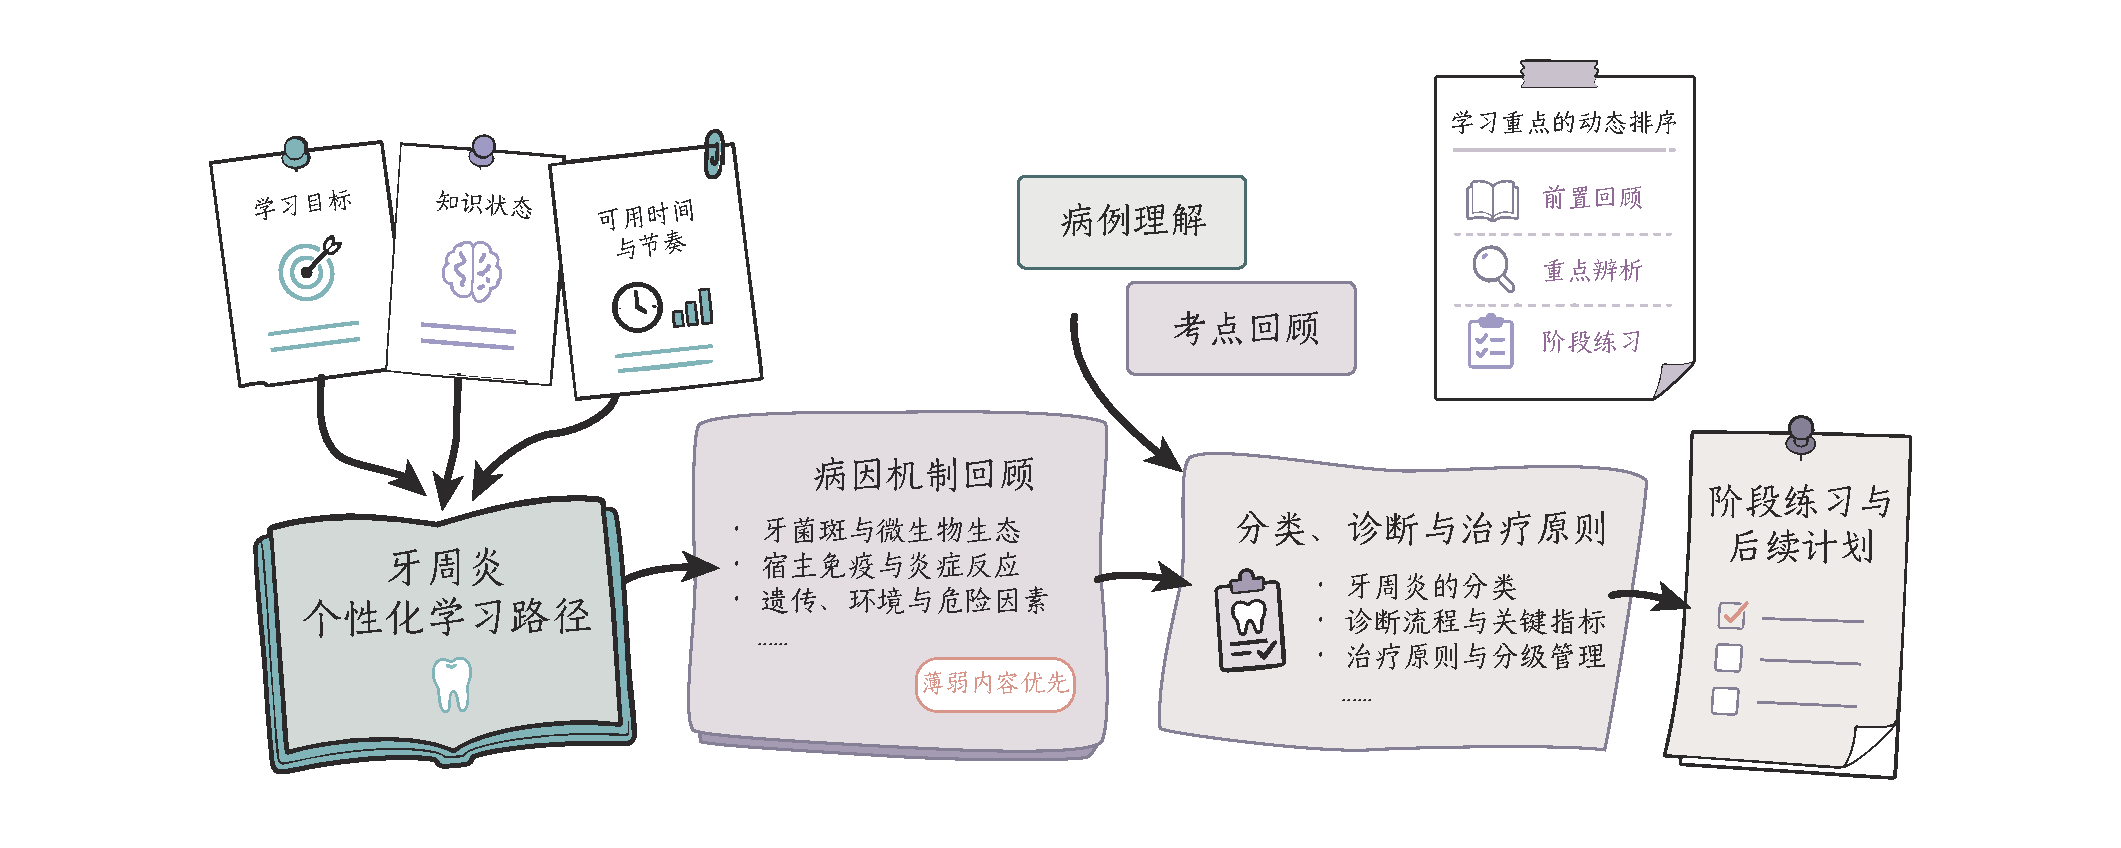
\includegraphics[width=\linewidth]{personalized-path-generation.pdf}
  \caption{个性化学习路径生成示例（以牙周炎为例）}
  \label{fig:personalized-path-generation}
\end{figure}

以牙周炎主题为例，系统可以将牙周组织基础、病因机制、分类与临床表现、诊断标准、治疗原则和维护阶段组织为连续学习单元。当画像显示学习者对基础病因概念掌握不足时，系统会在机制学习之前配置回顾任务。当目标为考试复习时，治疗原则学习之后可安排阶段性测评。图\ref{fig:personalized-path-generation}以这一过程说明知识结构、个人目标与行为状态如何共同影响学习路径。

\subsection{学习计划的长期节奏反馈}

学习计划推荐模块从近期画像和长期学习记忆中读取测评偏好、计划需求、薄弱点和掌握度等画像信息，生成面向下一阶段的任务列表并持续更新。任务完成、延期和计划修改等执行状态会作为学习事件写入节奏类学习记忆，为系统重新判断任务密度和优先级提供依据。OralSage 既利用已有画像形成初始安排，也持续吸收学习者的真实执行表现，使学习计划能够在长周期中保持可调整性。

\begin{table}[H]
  \centering
  \caption{学习计划推荐的输入与输出}
  \label{tab:study-plan-io}
  \begin{tabularx}{\linewidth}{p{0.24\linewidth}X}
    \toprule
    类型 & 内容 \\
    \midrule
    输入画像 & 学习目标、每日时间、计划支持需求、有效学习风格与执行节奏 \\
    输入学习状态 & 当前课程进度、KG 节点掌握度、薄弱点、错题和近期会话 \\
    输入计划状态 & 待完成任务、延期任务、完成记录与计划日期 \\
    输出任务 & 继续学习、薄弱点复习、低掌握节点回顾、定向练习、阶段测评和自定义计划 \\
    反馈写入 & 任务完成、延期与课程推进进入 L1 事件，并更新节奏类长期记忆 \\
    \bottomrule
  \end{tabularx}
\end{table}

\subsection{计划执行}

学习计划生成后，学习者可以在月历中查看计划分布，选择具体日期查看待办任务，也可以从总控对话中直接采纳系统生成的计划草案。面对个人时间变化，学习者可以根据实际安排补充、修改或删除任务，并始终保留计划执行与调整的主动权。

计划推荐全面覆盖课程进度、薄弱点复习、低掌握度内容回顾、补学任务、错题练习和阶段总结等学习场景。推荐过程优先读取近期学习行为和任务状态，使当日任务与正在进行的课程、尚未解决的薄弱内容以及已经延期的事项形成关联。以根尖周炎课程为例，当学习者完成“定义与疾病本质”后，计划可以安排后续的病因与危险因素学习。若阶段练习暴露出诊断辨析困难，计划会将临床表现与检查要点的回顾放到更靠前的位置，并附带对应练习。

任务的完成、延期和修改情况会被记录到学习记忆中，为系统判断当前任务量和学习节奏是否适配提供依据。持续完成能够为当前计划节奏提供正向信号，延期或反复修改则提示系统重新评估单日负荷和任务优先级。学习计划由此连接课程资源与真实执行行为，使后续安排能够参考学习者实际完成任务的情况。

\begin{figure}[H]
  \centering
  \begin{tikzpicture}[
    node distance=9mm and 8mm,
    planstep/.style={draw=black!70, rounded corners=2pt, fill=black!4, minimum width=28mm, minimum height=10mm, align=center, font=\small},
    focus/.style={draw=black!78, rounded corners=2pt, fill=chfiveaccent, minimum width=30mm, minimum height=11mm, align=center, font=\small\bfseries},
    flow/.style={->, >=stealth, thick, draw=black!78}
  ]
    \node[planstep] (state) {学习目标、掌握状态\\与可用时间};
    \node[focus, right=of state] (recommend) {当日计划推荐};
    \node[planstep, right=of recommend] (adopt) {采纳、修改\\与补充任务};
    \node[planstep, below=of adopt] (execute) {课程学习、复习\\与练习};
    \node[planstep, left=of execute] (feedback) {完成记录与\\调整信号};
    \draw[flow] (state) -- (recommend);
    \draw[flow] (recommend) -- (adopt);
    \draw[flow] (adopt) -- (execute);
    \draw[flow] (execute) -- (feedback);
    \draw[flow] (feedback) -- (state);
  \end{tikzpicture}
  \caption{学习计划连接资源推荐与每日学习执行}
  \label{fig:study-plan-resource-loop}
\end{figure}

\begin{table}[H]
  \centering
  \caption{学习计划中的任务类型及其资源组织}
  \label{tab:study-plan-resource-tasks}
  \begin{tabularx}{\linewidth}{p{0.22\linewidth}p{0.33\linewidth}X}
    \toprule
    任务类型 & 触发条件 & 面向学习者的资源安排 \\
    \midrule
    继续课程 & 当前主题尚有后续单元 & 进入下一节讲义、讲解和相关课件 \\
    薄弱点复习 & 追问、错因或测验显示理解缺口 & 回顾对应小节、易混辨析和定向练习 \\
    低掌握度回顾 & 某些知识内容的掌握状态偏低 & 优先复习基础概念和关键判断线索 \\
    补学任务 & 已安排任务未在计划日期完成 & 重新安排学习时段并保持原有学习顺序 \\
    阶段总结与练习 & 完成多个连续学习单元 & 组织阶段测试、解析和后续学习建议 \\
    \bottomrule
  \end{tabularx}
\end{table}

\section{个性化讲义与互动讲解}

学习者进行课程知识点学习时，系统会根据知识点和学习画像生成个性化讲义。每节讲义围绕当前学习单元组织概述、核心要点、临床病例、易混概念和章节过渡，帮助学习者明确本节任务，理解疾病机制和病理原因。病例内容进一步将抽象概念放入就诊情境，引导学习者辨析相近疾病、相似表现和常见误判。

对于基础尚需巩固的学习者，讲解从概念定义和病因机制进入，并通过病例连接临床表现。对于备考导向的学习者，讲解会更早呈现诊断线索、易混点和考查重点。对于希望理解临床应用的学习者，病例与治疗原则获得更充分的说明。学习者还可以围绕当前小节提出问题，在保持课程主线的前提下获得针对性解释。

这种组织方式与医学教育中强调案例化学习和问题驱动理解的方向相契合\cite{wei2025aipbl,sharmin2025oralhealthllm}。它使同一主题既保留医学知识的完整脉络，也允许学习者沿自己需要的深度和节奏进入内容。

\begin{figure}[H]
  \centering
  \begin{tikzpicture}[
    item/.style={draw=black!70, rounded corners=2pt, fill=white, minimum width=0.70\linewidth, minimum height=8mm, align=left, font=\small},
    emphasis/.style={draw=black!78, rounded corners=2pt, fill=chfiveaccent, minimum width=0.70\linewidth, minimum height=8mm, align=left, font=\small\bfseries},
    flow/.style={->, >=stealth, thick, draw=black!78}
  ]
    \node[item] (overview) {本节概述：明确当前学习任务与主题范围};
    \node[item, below=6mm of overview] (points) {核心要点：根据课程目标组织概念、机制和判断线索};
    \node[item, below=6mm of points] (case) {临床病例：将知识放入诊断和治疗情境};
    \node[emphasis, below=6mm of case] (confusion) {易混概念：突出学习者需要重点辨析的内容};
    \node[item, below=6mm of confusion] (next) {章节过渡：引导进入下一项个性化学习任务};
    \draw[flow] (overview) -- (points);
    \draw[flow] (points) -- (case);
    \draw[flow] (case) -- (confusion);
    \draw[flow] (confusion) -- (next);
  \end{tikzpicture}
  \caption{个性化分节讲义的学习组织方式}
  \label{fig:personalized-handout-structure}
\end{figure}

\begin{table}[H]
  \centering
  \caption{不同学习需要下的讲解组织重点}
  \label{tab:personalized-explanation}
  \begin{tabularx}{\linewidth}{p{0.23\linewidth}p{0.34\linewidth}X}
    \toprule
    学习需要 & 讲解组织重点 & 对学习者的支持 \\
    \midrule
    基础理解 & 概念定义、病因机制与层级关系 & 建立稳定的知识框架 \\
    考试复习 & 考点、易混判断和临床题干线索 & 提升辨析效率与应试准备度 \\
    临床应用 & 病例、检查结果、诊断依据和治疗原则 & 连接理论知识与临床思维 \\
    查缺补漏 & 薄弱内容、错因和定向回顾 & 聚焦个人理解缺口 \\
    \bottomrule
  \end{tabularx}
\end{table}

多媒体学习理论指出，学习材料需要帮助学习者在有限注意资源下组织关键信息\cite{mayer2021multimedia}。基于这一思路，OralSage 将长篇医学叙述转化为适合不同复习节奏的资源组合。

口腔医学知识包含疾病机制、诊断依据和治疗原则等细密内容，也强调概念之间的关联与临床判断的整体脉络。OralSage 围绕同一学习单元组织分节讲义、结构化课件、知识结构图和可播放语音，使学习者能够在文字阅读、视觉梳理与语音收听之间切换。多种资源围绕统一课程主线展开，有助于学习者在不同复习场景中保持理解的连续性。

每套课程会生成完整的知识结构图，呈现主题、学习单元与核心概念之间的关系，帮助学习者从局部内容回到疾病知识的整体框架。配套的 PPT 课件将当前小节的标题、导语和核心要点整理为层次清晰的知识卡片，配套语音则将课程内容延展为连续的听觉复习材料，支持学习者在通勤、间歇和睡前等碎片化时间中继续复习。

例如，图\ref{fig:personalized-ppt-preview}展示了“根尖周炎系统学习路径”的课件预览页。该页围绕“定义与疾病本质”展开，将规范定义、疾病本质与急慢性表现的连续性组织为三张要点卡片。学习者可以通过课件快速回顾核心内容，再结合知识结构图与语音讲解进一步梳理疾病机制和临床表现之间的联系。

\begin{figure}[H]
  \centering
  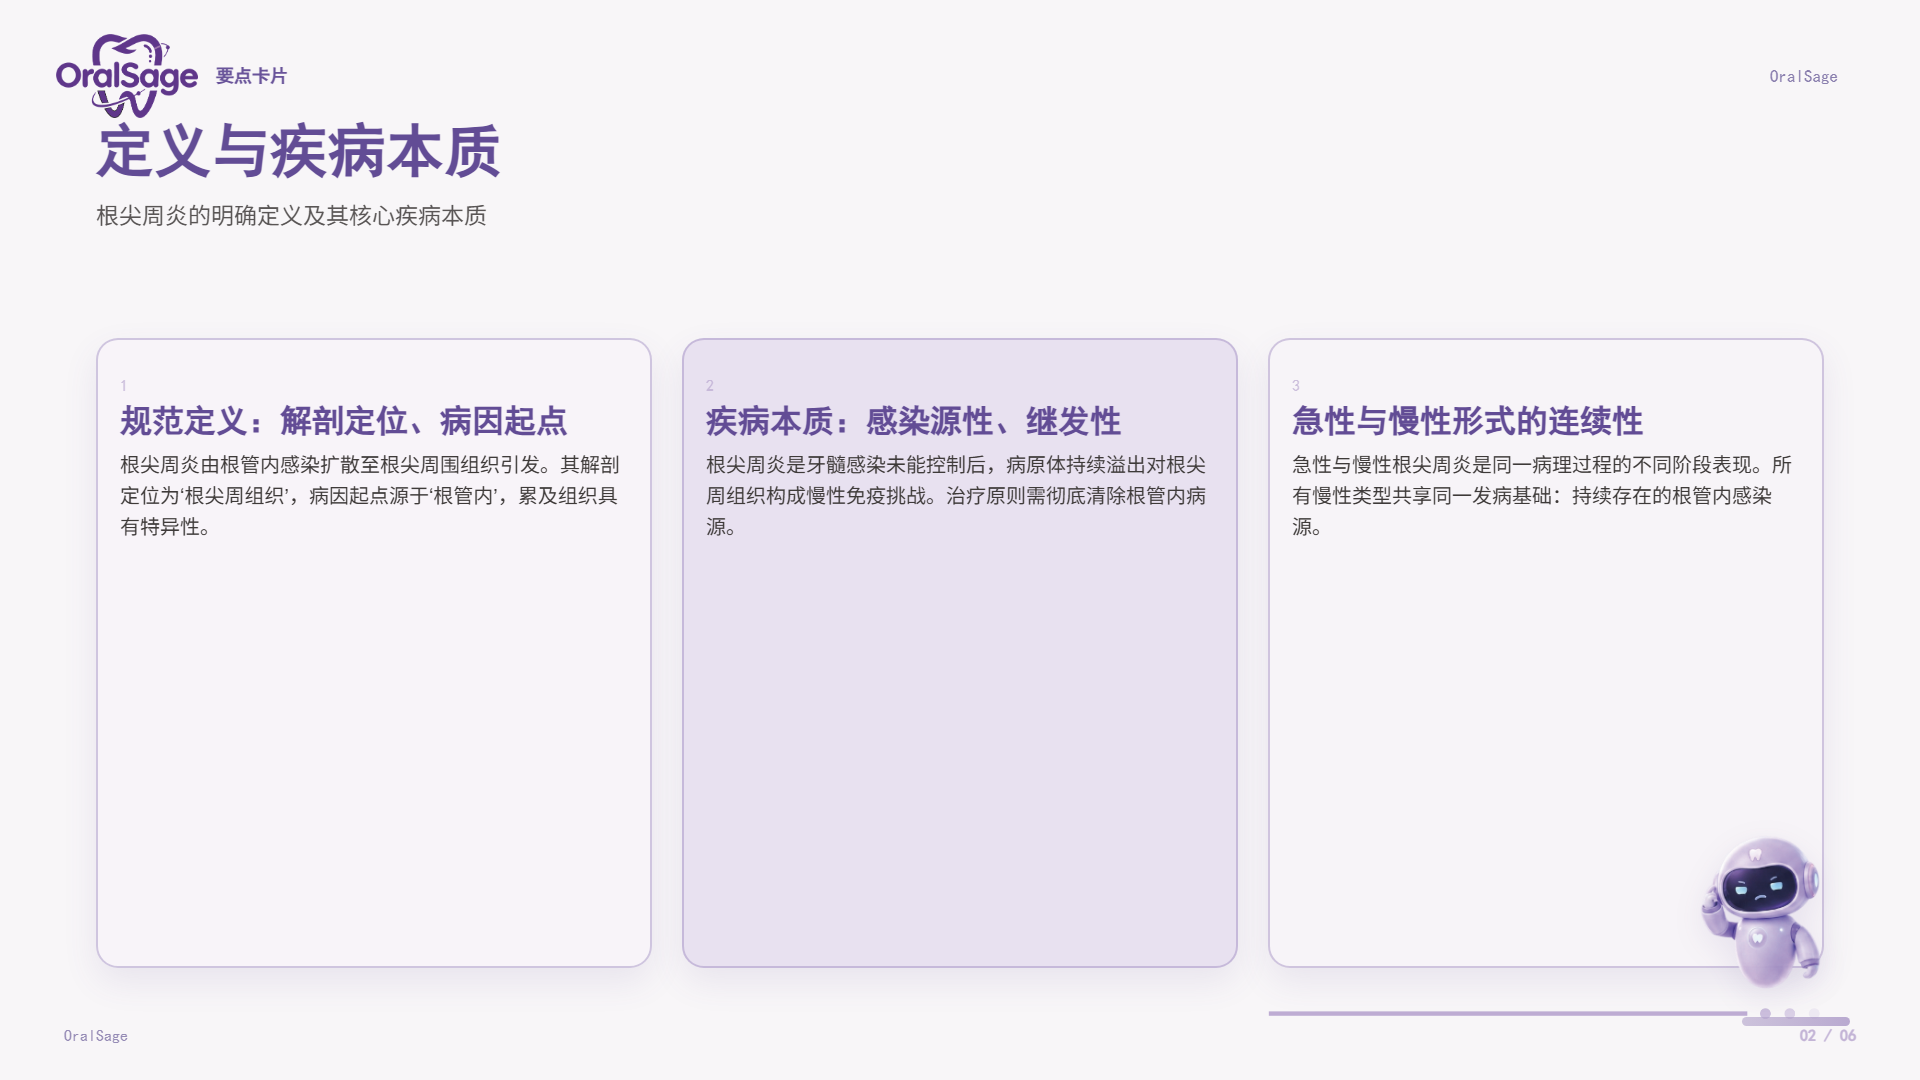
\includegraphics[width=\linewidth]{resource-ppt-preview.png}
  \caption{根尖周炎个性化课程中的结构化课件示例}
  \label{fig:personalized-ppt-preview}
\end{figure}

\begin{table}[H]
  \centering
  \caption{多模态资源对个性化复习的支持}
  \label{tab:multimodal-personalization}
  \begin{tabularx}{\linewidth}{p{0.20\linewidth}p{0.30\linewidth}X}
    \toprule
    资源形式 & 适合的学习节奏 & 学习支持 \\
    \midrule
    结构化课件 & 集中浏览和阶段回顾 & 快速定位当前主题与核心判断线索 \\
    知识结构图 & 学习前预览和考前梳理 & 建立主题全貌，识别前后知识关系 \\
    连续语音 & 通勤、间歇和睡前复习 & 利用碎片时间维持学习连续性 \\
    互动讲解 & 有疑问或需要深入理解时 & 根据当前困惑补充解释与例证 \\
    \bottomrule
  \end{tabularx}
\end{table}

\subsection{讯飞长文本语音合成}

语音资源以已经生成的课程讲稿为输入，不另行生成与讲义无关的内容。系统将 Tutor 讲解文本按照课程节点和讲稿片段组织为语音任务，服务端调用讯飞长文本语音合成 API 完成异步生成，再将音频文件保存到对应学习会话的资源目录中。部署版本使用中文发音人 \texttt{x4\_mingge}，输出 MP3 文件，并通过音频资源记录返回播放路径。

长文本语音合成采用“创建任务—查询状态—下载结果”的流程。这样既适合课程讲义和连续讲解等较长文本，也便于在前端先展示课程内容、再等待音频资源就绪。语音与讲义、Tutor 讲解共享同一课程节点，保证学习者在文字阅读、视觉回顾和听觉复习之间切换时仍处于同一学习主题。

\section{个性化练习与反馈}

个性化学习资源需要以练习检验理解，以反馈调整后续重点。小节练习紧跟当前学习内容，帮助学习者主动回忆和辨析关键知识。阶段测试覆盖多个连续单元，用于检查学习者对主题的整体掌握。根尖周炎真实课程会话已经形成五题阶段测试，题目通过临床情境、检查结果和治疗选择考查诊断线索与治疗原则的综合应用。

学习者提交答案后，系统提供得分、解析、薄弱内容提示和下一步建议。答题正确能够确认当前学习重点，答题失误则引导学习者回到相关小节，重新理解概念、病例或易混判断。对于反复出现的薄弱内容，后续课程更强调相应的讲解和练习。资源生成能够随着学习表现持续调整，并在后续安排中体现新的学习重点。

\begin{figure}[H]
  \centering
  \begin{tikzpicture}[
    node distance=14mm,
    box/.style={draw=black!70, rounded corners=2pt, fill=white, minimum width=29mm, minimum height=10mm, align=center, font=\small},
    focus/.style={draw=black!78, rounded corners=2pt, fill=chfiveaccent, minimum width=29mm, minimum height=10mm, align=center, font=\small\bfseries},
    flow/.style={->, >=stealth, thick, draw=black!78}
  ]
    \node[box] (learn) {当前学习重点};
    \node[box, right=of learn] (quiz) {小节练习};
    \node[box, right=of quiz] (exam) {阶段测试};
    \node[focus, below=of exam] (feedback) {得分与薄弱内容};
    \node[focus, left=of feedback] (adapt) {后续资源调整};
    \draw[flow] (learn) -- (quiz);
    \draw[flow] (quiz) -- (exam);
    \draw[flow] (exam) -- (feedback);
    \draw[flow] (feedback) -- (adapt);
    \draw[flow] (adapt) -- (learn);
  \end{tikzpicture}
  \caption{练习反馈驱动的资源动态调节}
  \label{fig:personalized-feedback-loop}
\end{figure}

\begin{table}[H]
  \centering
  \caption{练习反馈对资源调整的作用}
  \label{tab:personalized-feedback-effects}
  \begin{tabularx}{\linewidth}{p{0.22\linewidth}p{0.32\linewidth}X}
    \toprule
    学习表现 & 后续资源变化 & 学习意义 \\
    \midrule
    当前内容掌握良好 & 继续推进后续单元与综合测试 & 保持学习效率和挑战度 \\
    某一知识点理解薄弱 & 增加对应讲解、易混辨析和定向练习 & 集中解决真实理解缺口 \\
    多个单元出现困难 & 调整复习顺序并回顾基础内容 & 重新建立必要的知识基础 \\
    节奏执行不稳定 & 减少单次任务量并强化碎片化复习 & 提升学习计划的可持续性 \\
    \bottomrule
  \end{tabularx}
\end{table}

OralSage 由此将学习画像转化为可执行的学习路径和计划，并围绕各学习单元组织讲义、讲解、多模态材料与练习。学习者的实际学习表现又会反向影响后续资源重点，使个性化不只体现在首次生成，而是持续贯穿课程推进、练习反馈和复习调整过程。


% !TeX root = ../main.tex

% !TeX root = ../main.tex
\chapter{知识库}
\label{sec:knowledge-guardrail}

本章介绍 OralSage 从多源医学资料到智能体知识服务的完整构建链路。教材、临床规范、诊疗手册和题库经过结构恢复与语义处理后，分别形成医学文本、知识图谱和题目对象；这些对象通过多路索引与来源关系连接，再由 KAGSolver 为课程规划、资源生成、教学讲解、智能答疑和学习测评提供带有知识关系与来源位置的检索上下文。

\section{数据输入与预处理}

本项目收集了14本口腔医学专业课程教材、口腔医学领域专家共识与临床规范、《默沙东诊疗手册》以及口腔医师执业考试真题作为知识库基础资料输入，具体资料说明如表~\ref{tab:kb-source-overview}所示。

{\small
\renewcommand{\arraystretch}{1.08}
\begin{longtable}{p{0.27\linewidth}p{0.63\linewidth}}
  \caption{知识库基础资料}\label{tab:kb-source-overview}\\
  \toprule
  资料类型 & 内容与使用范围 \\
  \midrule
  \endfirsthead
  \multicolumn{2}{c}{续表~\thetable}\\
  \toprule
  资料类型 & 内容与使用范围 \\
  \midrule
  \endhead
  \bottomrule
  \endfoot
  口腔医学教材 & 理论学习基础，并为知识图谱和教学内容提供教材依据 \\
    专家共识与临床规范 & 实操规范，为诊疗选择、适用条件和风险控制提供权威依据 \\
    《默沙东诊疗手册》 & 补充各类疾病、药物、症状鉴别和跨学科的医学知识 \\
    口腔执业医师考试相关题库 & 课后练习和测试，支持薄弱点和知识盲区的识别 \\
\end{longtable}
}

数据输入先按照资料形态完成基础预处理，保留表格、版面、文字与层级结构，并统一整理文档、页面、片段和段落位置。文本内容按照引文范围和主题边界合并为语义单元，教材知识图谱、医学文本和题库随后建立双向联系，再生成统一检索语料以及稀疏、向量和图关系索引。标识与引用校验、重复内容标记、链接验证和质量检查随各处理步骤执行，整体流程如图~\ref{fig:data-processing-pipeline} 所示。

\begin{figure}[H]
  \centering
  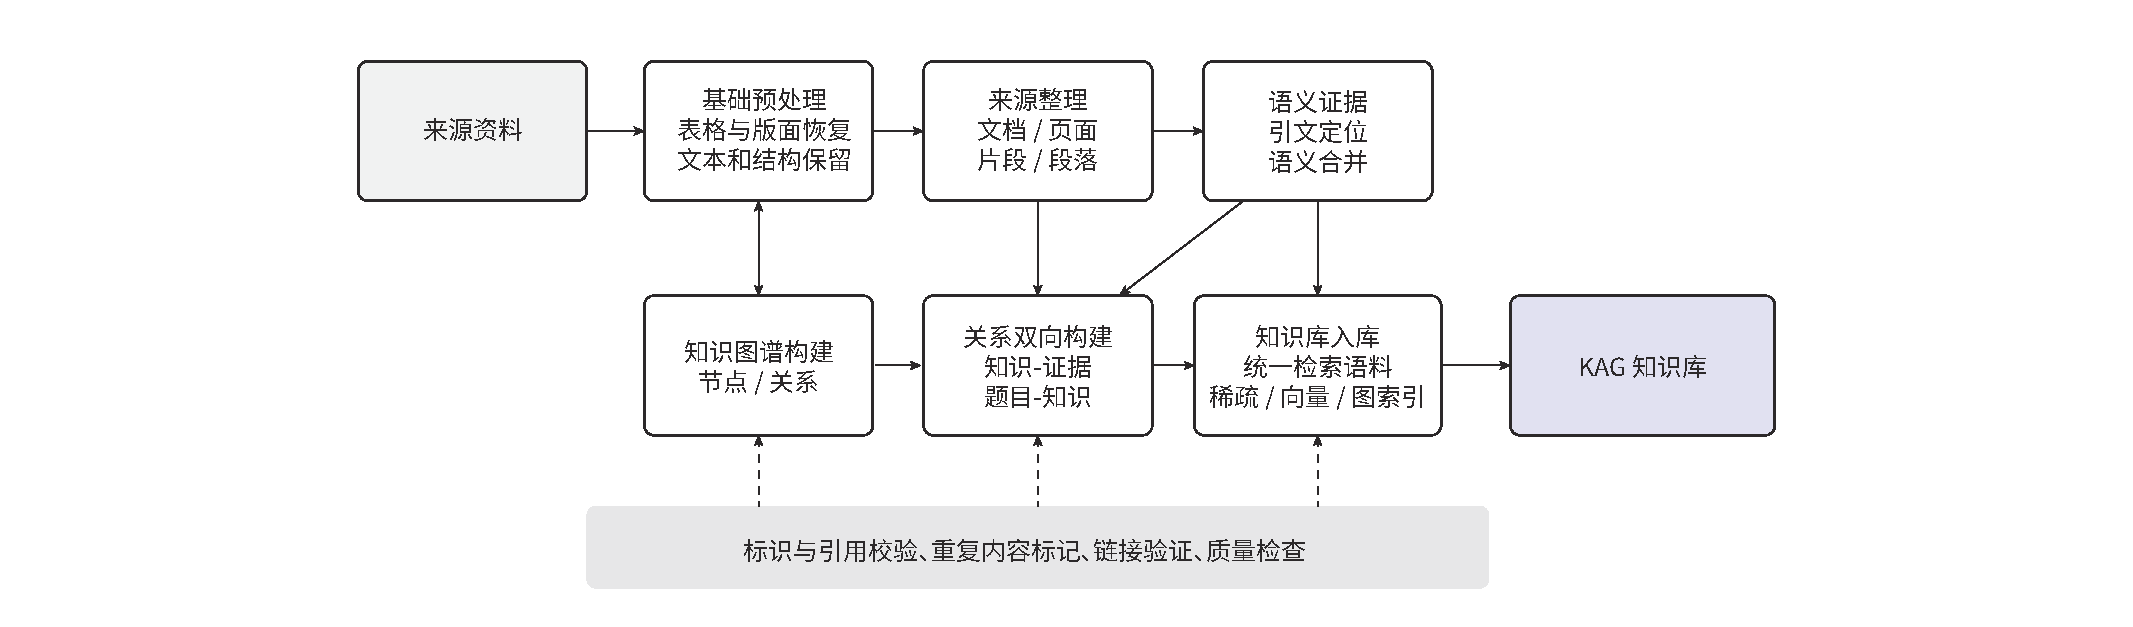
\includegraphics[trim=150 8 150 8,clip,width=\linewidth]{kb-data-process.pdf}
  \caption{OralSage 多源数据处理流程}
  \label{fig:data-processing-pipeline}
\end{figure}

\subsection{口腔医学教材}

项目收集整合了 14 本口腔医学权威教材，这些教材多选自“人卫十三五”规划系列，涵盖口腔医学的临床诊疗、生物机理、材料科学及全流程治疗方案等核心领域，侧重于基础理论的深度阐释和学科体系的完整性，构成了系统的“学术基础层”，为学习内容提供完整的学科体系、稳定的术语规范和教学级知识依据。教材具体说明如表~\ref{tab:textbook-inputs}所示。
{\small
\renewcommand{\arraystretch}{1.08}
\begin{longtable}{p{0.27\linewidth}p{0.10\linewidth}p{0.49\linewidth}}
  \caption{口腔医学教材输入清单}\label{tab:textbook-inputs}\\
  \toprule
  教材 & 版本 & 主要知识范围 \\
  \midrule
  \endfirsthead
  \multicolumn{3}{c}{续表~\thetable}\\
  \toprule
  教材 & 版本 & 主要知识范围 \\
  \midrule
  \endhead
  \bottomrule
  \endfoot
  《儿童口腔医学》 & 第5版 & 儿童口腔生长发育、龋病、牙髓根尖周病与牙外伤 \\
  《口腔材料学》 & 第6版 & 材料组成、理化性能、生物学性能与临床选择 \\
  《口腔颌面外科学》 & 第8版 & 颌面部疾病、创伤、肿瘤、诊断与外科操作 \\
  《口腔颌面医学影像诊断学》 & 第7版 & 影像检查原理、正常影像表现与疾病影像诊断 \\
  《口腔临床药物学》 & 第5版 & 口腔常用药物、药理作用、适应证与用药风险 \\
  《口腔黏膜病学》 & 第5版 & 口腔黏膜疾病的病因、表现、诊断与治疗 \\
  《口腔生物学》 & 第5版 & 口腔组织的细胞、分子、微生态与生物学机制 \\
  《口腔修复学》 & 第8版 & 牙体、牙列及颌面缺损的修复设计与临床流程 \\
  《口腔预防医学》 & 第7版 & 口腔流行病学、疾病预防、健康教育与社区保健 \\
  《口腔正畸学》 & 第7版 & 错颌畸形的病因、诊断、矫治设计与生物力学 \\
  《口腔种植学》 & 第1版 & 种植生物学、手术、修复设计与并发症管理 \\
  《口腔组织病理学》 & 第8版 & 口腔组织发育、正常结构及疾病病理变化 \\
  《牙体牙髓病学》 & 第5版 & 龋病、牙体硬组织病、牙髓病与根尖周病 \\
  《牙周病学》 & 第5版 & 牙周组织、牙周疾病的诊断、治疗与维护 \\
\end{longtable}
}

由于口腔医学各学科之间具有较强的知识依赖，真实的口腔医学课程学习中，学生往往需要建立起清晰的知识架构，同步理解正常组织结构、生物学机制、病理变化和临床表现。因此，本项目在处理教材资料时保持从基础理论到临床应用的连续知识脉络，将疾病分类、专业术语和诊疗原则经过系统编排，通过连续的章节论述，保留概念产生的背景与前后联系，避免零散知识片段带来的割裂感。

由于教材原始资料多为图片扫描版PDF，无法直接进行文本检索，为了将教材中的学科结构和医学内容转换为可检索定位的教学证据，本项目具体处理方法如下。

\noindent{（1）图像增强与 OCR 识别}
\nopagebreak[4]

教材 PDF 的原始扫描件存在分辨率不一、噪点较多等问题。首先对扫描页进行图像增强和高清压缩，随后使用开源 PaddleOCR 工具批量提取文字，并将识别结果统一转换为 UTF-8 文本。针对医学文档中常见的复杂排版和专有名词，对识别结果进行人工抽检和校对，将非图片内容转化为可编辑的文字模态信息。

\noindent{（2）保留章节结构与来源位置}

教材知识依赖章、节和局部标题形成连续语境，仅保存正文会丢失知识所属位置。因此，在对文字进行提取时保留章标题、节标题、局部标题、图题、表题和页码，并为教材、页面和局部文本片段建立逐级位置关系。

\noindent{（3）语义分块与索引复用}

由于 OCR 文本中的换行可能来自真实段落，也可能来自页面排版。本项目在处理时根据空行、章节编号、短标题、括号标题、编号条目和图表提示判断行的类型，同时清理重复页眉、页码和低信息噪声。对属于同一语句的连续行进行重新连接，章标题、节标题和局部标题则单独保留，并按出现顺序形成标题路径，使后续正文能够继承距离最近的有效标题。此外，按照语义构建分块，优先在新的章、节或主要标题处结束当前语义块，在必要时调整块的长度，确保按照知识逻辑进行组织，为后续知识图谱节点、检索结果和生成内容保留可定位的教材内容。索引构建后通过了召回验证，重点检查了专业术语和疾病分类的检索准确率，确保知识库在实际使用中具备基本可靠性。

\subsection{专家共识与临床规范}

本项目收集了 30 项与临床实践紧密相关的口腔医学专家共识、诊疗指南和操作规范，其中包括《创伤性周围性面瘫外科治疗专家共识》《单侧唇裂诊疗指南》《牙周龈下刮治和根面平整术操作规范》和《口腔种植体周病管理专家共识》等资料（详见附件）。涉及学科覆盖口腔颌面外科、牙体牙髓、牙周、修复、正畸、种植、口腔黏膜、儿童口腔和急诊处置。

专家共识代表了行业内的“金标准”，具有表述规范、逻辑严密、指导性强的特点。这部分数据作为临床规范，为适应证判断、治疗方案制定和操作风险控制提供权威依据。专家共识的补充，可以进一步回答特定条件下应选择何种方案、何时不宜实施以及操作中需要控制哪些风险。在处理临床应用题、诊疗原则和操作规范问题时，以临床规范为约束，能够减少智能体仅凭一般医学知识推演临床结论的风险，增强诊疗内容的严谨性。

专家共识和诊疗指南多以 PDF 格式输入，存在大量页眉页脚、分页残留和多栏分布文字，为了最大限度保留专家共识和数据指南材料的医学严谨性并适配知识库检索，制定以下处理策略。

\noindent{（1）文本清理与格式矫正}

处理过程中需要清理重复标点与异常空白，并按照栏区恢复双栏或多栏页面的阅读顺序。对于跨页但语义连续的段落，需要重新连接前后内容，使推荐意见及其适用条件能够保持完整。

\noindent{（2）临床条款结构保留}

专家共识在引用时需要与适用条件和操作要求共同出现，缺少上下文容易改变临床含义，且该类资料一般以条款式或分层级小节形式呈现，章节之间逻辑紧密，但每一段内部内容相对独立，较适合自动切分。因此，在处理过程中保留“推荐意见”“注意事项”“适应证”“禁忌证”和“操作步骤”等标题及其条款编号，并将标题与后续正文共同组织。经过处理后，治疗建议、适用范围和风险提示仍然保持明确对应关系。

\noindent{（3）表格语义重组}

诊疗指南中的表格将适用条件、操作要求和评价结果分置在不同列，逐单元格提取会破坏同一条临床信息的联系。因此，处理时按照数据行或完整逻辑单元转写表格，使同一项诊疗条件和结论进入连续文本，并保留表题及其所在章节，从而为后续分块提供完整语义。

\subsection{默沙东诊疗手册}

《默沙东诊疗手册》作为全球连续出版时间最长的综合性医学手册之一，自1899年首次发行以来，已成为世界上使用最广泛的医学信息资源之一。其核心特征包括内容全面性、权威可靠性、版本多样性、免费获取性和更新及时性，为医疗专业人士和普通公众提供科学准确的医学信息支持，在本项目中作为通用医学知识的重要来源。

口腔症状可能与感染、免疫、代谢和肿瘤等全身性问题相关，患者用药也会影响口腔表现与治疗选择。手册中的疾病百科、症状解析、检查方法、治疗原则和药物信息，能够补充基础病理知识缺失，使系统能够把口腔专科问题放入更完整的医学背景中理解。基础疾病查询、症状鉴别和药物咨询可从中获取跨学科线索，教材中的口腔知识也能由此联系炎症反应、组织损伤和全身疾病机制。

为了将手册内容适配到本项目知识库检索系统中，制定以下数据处理方法。

\noindent{（1）数据采集与格式处理}

使用爬虫技术将默沙东诊疗手册的公开内容完整爬取，统一文字编码与空白格式，并清理导航、模板和其他网页噪声，初步整理为JSONL格式以便存储。

\noindent{（2）保留疾病条目层级}

疾病条目中的概述、症状、检查、治疗和药物信息具有明确的从属关系，脱离标题后容易失去医学语境。因此，处理过程中按照网页标题层级组织正文，并把疾病名称和局部主题补充到对应文本中，使每段内容仍能确定所属疾病及其医学主题，为全身疾病口腔表现、药物作用、症状鉴别和跨学科概念解释提供补充依据。


\subsection{口腔执业医师考试相关题库}

题库面向口腔医学执业医师考试相关科目，共收集 3,161 道选择题，覆盖 12 个学科。题量分布见表~\ref{tab:question-inputs}，其中临床医学题目用于补充口腔疾病相关的全身医学基础。

\begin{table}[H]
  \centering
  \caption{执业医师考试相关题库的学科分布}
  \label{tab:question-inputs}
  \begin{tabularx}{\linewidth}{X r X r}
    \toprule
    学科 & 题量 & 学科 & 题量 \\
    \midrule
    牙体牙髓病学 & 651 & 口腔颌面外科学 & 549 \\
    口腔修复学 & 436 & 牙周病学 & 435 \\
    临床医学 & 410 & 口腔黏膜病学 & 204 \\
    儿童口腔医学 & 120 & 口腔组织病理学 & 106 \\
    口腔预防医学 & 104 & 口腔解剖生理学 & 72 \\
    口腔材料学 & 44 & 口腔颌面医学影像诊断学 & 30 \\
    \midrule
    合计 & \multicolumn{3}{r}{3,161} \\
    \bottomrule
  \end{tabularx}
\end{table}

题干将病史、症状、检查结果和治疗条件组织为具体的临床情境，要求学习者能够识别影响诊断或治疗选择的关键信息，并运用相应知识完成判断。该类题目精心设计了大量混淆项，不同选项之间往往只有疾病阶段、适用条件或处置原则上的细微差别，能够有效暴露出学习者的真实学习情况。学习者在答题过程中如果进行了错误的选择，在一定程度上能体现其该类知识点上的薄弱之处，系统会予以记录并更新学习画像，为学习者提供针对性反馈。

为了从题库 PDF 中得到题目结构完整、答案对应准确的标准记录，本项目具体处理方法如下。

\noindent{（1）恢复 PDF 分栏顺序}
\nopagebreak[4]

题库 PDF 采用双栏排版，直接提取容易把相邻题目的题号、题干和选项交叉拼接。程序在识别文字前按照栏区恢复阅读顺序，并检查题号与选项是否连续，使每道题目的内容保持在同一记录中。

\noindent{（2）对齐题目、答案与解析}

项目所收集到的资料中，题目和解析大多分开编排，答案汇总表与逐题解析也采用不同格式。在处理时需要识别题目页、答案汇总表和解析段落，再按照科目、章节和章节内题号建立对应关系。经过对齐后，每道题都能够同时关联题干、选项、答案和解析，并保留其在 PDF 中的题目块、答案块和解析块位置。


\noindent{（3）建立题目与知识点关联}

首先在同名科目和对应章节内匹配知识图谱中的核心知识、支撑知识和概念，再根据节点归属关系连接到正式核心知识点。处理后形成 3,161 个题目对象和 6,287 条题目到知识点的关系，使题目能够沿知识节点访问相应教材证据，并为练习推荐、错因分析和掌握度更新提供结构化依据。


\section{知识图谱构建}

完成教材文本整理和章节位置恢复后，项目使用 OralPath KG-Forge 构建口腔医学知识图谱。该流程借鉴编译系统的处理方式，将版本化教材与指南作为输入，将书、章、节组成的文档结构树作为章节映射，将受控医学 Schema 作为类型规则，并以片段标识、双页码和连续引文记录知识来源。模型抽取结果先写入 Evidence-to-Graph Intermediate Representation（EGIR），经过医学审议与确定性编译后，再生成口腔医学知识图谱节点。

\subsection{自动化持续构建}

构建过程中，系统能够实现新教材接入、教材版本更新和指定章节重建。Corpus Watcher 为文档、章节和局部片段计算内容指纹，并与上一次构建清单比较，从而确定需要处理的章节范围。文档随后解析为书、章、节组成的结构树，每个层级保留文档版本、PDF 页序、印刷页码和局部片段位置，章节范围按照同级标题边界确定，后续抽取能够始终在明确的教材范围内进行。

Incremental Build Planner 根据内容指纹和来源依赖关系生成持久化任务 DAG，将构建批次拆分为章节抽取、章节检查、跨章节归并和制品发布等任务。彼此独立的章节由 Worker Pool 并行处理，来源内容、Schema 版本和抽取配置共同形成任务幂等键。内容未发生变化的章节复用既有结果，发生变化的章节及其关联关系进入重建流程，使多本教材能够按照最小必要范围持续更新。

\subsection{Schema 引导抽取与 EGIR 生成}

提取章节过程中，首先识别普通医学、指南与防护、绪论与概述等不同内容模式，再选择对应的节点类型和关系集合。普通医学章节围绕疾病、病因、病原体、风险因素、症状、体征、影像表现、病理变化、诊断方法、治疗、并发症和解剖结构组织知识。放射防护、操作安全和规则型章节增加防护原则、防护措施、剂量限制、设备要求、操作规则和辐射风险等类型，合理处理规范化内容。

模型根据章节文本生成 EGIR，其中保存候选节点、原子医学陈述、补充概念、来源指针和抽取记录。每条候选陈述在生成时即关联连续引文、片段标识和页码位置，使实体、关系与教材内容从抽取阶段开始保持对应。书、章、节继续承担来源结构的组织功能，正式医学实体从核心知识层开始，章节标题不会混入疾病、治疗或诊断节点。

\subsection{节点与关系编译}

知识对象按照核心知识、支撑知识和补充概念分层组织，无法进入图谱的候选项同时保留处理原因。各层的编译要求见表~\ref{tab:kg-object-contract}。

\begin{table}[H]
  \centering
  \caption{知识图谱对象分层与编译要求}
  \label{tab:kg-object-contract}
  \begin{tabularx}{\linewidth}{>{\raggedright\arraybackslash}p{0.18\linewidth}p{0.40\linewidth}X}
    \toprule
    知识对象 & 医学内容 & 编译要求 \\
    \midrule
    核心知识 & 章节或节次重点讨论的疾病、解剖结构及医学主题 & 使用规范名称和受控类型，每个核心知识至少参与两条正式关系。 \\
    支撑知识 & 病因、症状、体征、影像、病理、诊断、治疗和并发症等关系对象 & 通过正式关系连接核心知识，每个支撑知识至少参与一条正式关系。 \\
    补充概念 & 来源明确且适合辅助解释，但难以使用受控谓词完整表达的内容 & 使用 \texttt{RELATE} 连接一至三个相关节点，并记录采用补充连接的原因。 \\
    舍弃候选 & 引文不完整、内容重复、缺少合理连接或图谱信息量较低的候选项 & 不写入正式节点与关系，同时保留候选内容、处理原因和对应引文。 \\
    \bottomrule
  \end{tabularx}
\end{table}

正式关系采用受控的主语、谓词和宾语结构。普通医学关系覆盖病因、病原体、风险因素、症状、临床体征、影像表现、病理特征、并发症、诊断方法、治疗方法、发生部位、鉴别对象和疾病亚型。指南与防护关系补充适用对象、前置要求、防护原则、防护措施、剂量限制、设备要求和风险降低等语义。编译程序同时检查谓词方向以及两端节点类型，使疾病与病因、疾病与诊断方法、操作规则与适用对象等关系保持一致的表达方式。

\subsection{医学审议与符号编译}

EGIR 依次经过医学抽取、类型复核、来源核验、图结构检查和综合裁决。医学抽取单元将连续文本拆为原子医学陈述并补全候选节点，类型复核单元检查节点类别、关系谓词和连接方向，来源核验单元判断连续引文能否完整支持一条主谓宾关系，图结构检查单元识别重复节点、自环、悬空连接和概念挂接异常，综合裁决单元据此确定正式关系、补充概念或舍弃候选。

完成审议的 EGIR 随后进入确定性编译步骤。程序依次规范实体名称和别名，检查节点与关系类型，核对片段、页码和连续引文，合并重复节点与完全相同的关系，并检查核心知识度数、支撑知识连接和补充概念挂接。可修正的名称、引用和连接问题进入一次有界修复，修正结果重新接受同一组检查。仍未满足结构要求的候选连同诊断信息进入隔离队列，其余章节可以继续完成构建与发布。

质量检查由 Schema 符合度、医学类型符合度、来源覆盖、引文支持、图结构完整性、概念连接完整性和构建可复现性共同组成。检查过程采用明确规则与结构化诊断，节点数量不会单独决定图谱质量。每条正式关系均保留片段标识、PDF 页序、印刷页码、连续引文和关系说明，使图谱中的医学陈述能够定位到对应教材内容。

\subsection{跨章节归并与交付}

各章节完成编译后，Resolution Job 根据规范名称、别名、节点类型和章节语境识别跨章节同名实体，并生成统一映射。章节内部的局部引用保持不变，单章节图谱可以独立读取，跨章节检索也能够识别指向同一医学实体的多个局部节点。该处理兼顾章节制品的独立性与全书范围内的术语一致性。

Publish Job 将章节 JSON、文档级索引和质量报告作为同一发布单元，解析检查完成后再登记正式版本。每次构建记录来源文档与版本、内容指纹、Schema 版本、流水线配置、制品摘要、质量报告和依赖快照。相同输入与配置对应相同的构建键，新版本以独立制品保存，使图谱生成过程具备清晰的版本链和来源记录\cite{w3c-prov-dm}。

系统同时维护局部片段到节点、关系和章节制品的依赖关系。教材版本或 OCR 文本发生变化时，Dependency Tracker 标记受影响的图谱对象，并由构建规划器重新处理相关章节与关系。未受影响的章节继续复用既有制品，从而完成按来源变化范围执行的增量更新。发布后的图谱节点、正式关系、补充概念、章节归属和来源位置随后进入 6.3 节的统一入库与索引构建流程。

\section{知识库入库与索引组织}

完成多源资料预处理和知识图谱构建后，将教材语义文本单元、临床规范文本、诊疗手册文本、知识图谱节点和题库题目进行知识库入库，核心工作包括检索对象组织、多路索引构建和知识关系连接，为后续 KAG 求解器提供候选召回、关系扩展和上下文基础。

\subsection{检索对象的统一组织}

多源资料入库后形成教材语义文本单元、临床规范文本、诊疗手册文本、知识图谱节点和题库题目五类检索对象。文本单元提供教材、规范和手册中的医学原文内容，知识图谱节点提供口腔医学概念、章节归属和关系结构，题库题目提供考查场景、选项解析和学习反馈依据。经过统一组织表示后，检索器能够在同一流程中处理医学正文、结构化知识和题库材料，并将不同来源的候选内容组织为面向 KAG 求解器的一致输入。

\subsection{多路索引的构建机制}

口腔医学查询包含明确术语、病例化描述、同义表达和关系推理需求。本项目围绕入库对象构建术语别名索引、稀疏倒排索引、稠密向量索引和图关系索引。四类索引分别承担名称匹配、词项匹配、语义匹配和关系扩展功能，其形式化表示为：

\begin{equation}
  \label{eq:multi-index-set}
  \mathcal{I}=\{\mathcal{I}_{\mathrm{alias}},\mathcal{I}_{\mathrm{sparse}},\mathcal{I}_{\mathrm{dense}},\mathcal{I}_{\mathrm{graph}}\}
\end{equation}

（1）术语别名索引。Alias Index 由知识节点的规范名称、常用别名、英文术语和专业缩写构成，采用字符串规范化与别名表匹配方式进行索引。其目的在于处理疾病名、操作名、解剖结构名和专业缩写等明确查询，并将查询直接映射到候选知识节点，为后续图扩展提供初始种子。

（2）稀疏倒排索引。BM25 Sparse Index 采用中文分词、英文数字识别和中文双字组合构建倒排结构，并按照 BM25 评分衡量查询词项与候选文本之间的匹配程度。该索引用于教材原文、题干关键词、数值条件和医学术语召回，能够保留精确词项匹配对医学检索的约束作用。

（3）稠密向量索引。BGE-M3 Dense Index 使用 BGE-M3 模型\cite{chen2024m3embedding}对入库对象进行语义编码，并通过归一化向量计算查询与候选对象之间的语义相似度。FAISS 进行相似向量检索功能，BGE-M3 负责文本表示生成。该索引用于同义表达、口语化问题和病例化描述召回，补充稀疏匹配难以覆盖的语义相关内容。

（4）图关系索引。Graph Index 保存知识节点、医学文本单元和题库题目之间的邻接关系，覆盖 KG adjacency、KG-Chunk links 和 Question-KG links 等关系。该索引用于从候选知识节点扩展到相关概念、医学原文和练习题目，并支持 KG path 输出、Graph-PPR 候选传播和来源定位。

\subsection{知识关系与来源关联}

入库阶段将知识图谱、医学文本和题库题目连接为能够遍历的关系结构。教材知识节点与医学文本单元之间建立知识到文本的关联，使知识点能够返回对应的原文材料。题库题目与知识节点之间建立考查关系，使练习推荐、错因分析和掌握度更新能够回到具体知识点。

医学文本单元继续保留资料、页码、span 和标题路径等来源信息。检索命中文本单元时，系统能够沿关联知识标识返回相关知识点。术语别名索引命中知识点时，系统能够沿关系结构获得相关医学文本和题目材料。图关系索引将这些连接组织为在线能够遍历的邻接结构，为 Graph-PPR、KG path 输出和引用定位提供基础。

\subsection{入库结果}

入库完成后，知识库形成了统一组织医学文本、结构知识、题库材料和来源位置的知识对象空间。专家共识和《默沙东诊疗手册》作为独立来源层保留各自的资料属性，用于补充口腔专科问题中的临床规范和通用医学参考。各类对象在入库阶段完成标识统一、关系连接和索引准备，具体在线召回、扩展与排序过程在 6.6 节中说明。

面向上层智能体，入库结果能够提供医学文本、相关知识点、关系路径和来源位置。不同智能体通过统一检索接口读取与当前任务相关的对象，具体调用方式在 6.6 节的 KAGSolver 与智能体调用部分说明。

\section{KAG 知识库架构}
本项目中的知识库需要同时支持课程规划、多模态资源生成、教学讲解、智能答疑和学习测评等任务。基于文本向量的检索方式难以同时表达教材章节关系、诊疗知识联系和题目考查关系，也难以让不同学习任务使用同一组知识对象。为此，项目采用基于 KAG 的知识库架构，沿用知识图谱与文本互索引、多路检索和图关系扩展等基础设计，并结合口腔医学资料特点补充教材章节组织、题目关联、来源属性和多智能体调用接口。

\subsection{KAG 基础架构与项目适配}

KAG 面向专业知识服务，将知识图谱的结构表达与向量检索的语义匹配能力结合起来，并通过适合大模型使用的知识表示、知识图谱与文本互索引、混合推理以及知识对齐，缩小文本相似度与知识推理相关性之间的差距\cite{liang2024kag}。本项目采用其中的结构化知识表示、双向索引和混合检索思路，以前期构建的口腔医学教材知识图谱组织学科范围与知识关系，通过结构化存储的医学文本保留专业表述，再通过多路检索与关系扩展为上层智能体整理学习上下文。

项目知识库分为知识表示、知识互索引、混合检索和知识服务四个部分。知识表示负责保存教材层级、知识点及医学关系；知识互索引负责连接知识节点、语义文本单元和考试题目；混合检索负责从不同匹配角度取得相关对象；知识服务则将结果整理为上层智能体能够按任务读取的统一上下文。针对口腔医学学习场景，项目进一步补充资料层级、题目到知识点的考查联系和多智能体调用接口，具体对应关系见表~\ref{tab:kag-adaptation}。

\begin{table}[H]
  \centering
  \caption{KAG 基础能力与 OralSage 场景适配}
  \label{tab:kag-adaptation}
  \begin{tabularx}{\linewidth}{p{0.22\linewidth}p{0.38\linewidth}X}
    \toprule
    KAG 基础能力 & OralSage 场景适配 & 支撑任务 \\
    \midrule
    结构化知识表示 & 以教材学科、章节和知识点层级组织口腔医学概念及其关系 & 学习顺序规划与知识范围控制 \\
    知识与文本互索引 & 建立知识点、医学内容和资料位置之间的双向联系 & 讲义生成、教学讲解与来源定位 \\
    混合检索与图扩展 & 联合术语、词项、语义向量和知识关系获取候选内容 & 病例化提问、同义表达与关联知识检索 \\
    知识服务输出 & 区分教材、临床规范、外部参考和题库的资料属性，并组合医学内容、知识节点、关系路径、引用位置和检索轨迹 & 多智能体调用、医学内容组织与学习评价反馈 \\
    \bottomrule
  \end{tabularx}
\end{table}

\subsection{知识库总体架构}

图~\ref{fig:kb-architecture} 将 KAG 知识库划分为知识库构建流、异构知识空间、KAG Solver 检索链路、来源与质量控制以及多智能体调用五个相互连接的区域。资料沿左侧构建流进入中央知识空间，查询从右侧检索链路获得经过组织的回答上下文，顶部智能体通过统一接口调用这些结果，底部的来源与质量控制为构建和检索过程提供限制条件。

\begin{figure}[H]
  \centering
  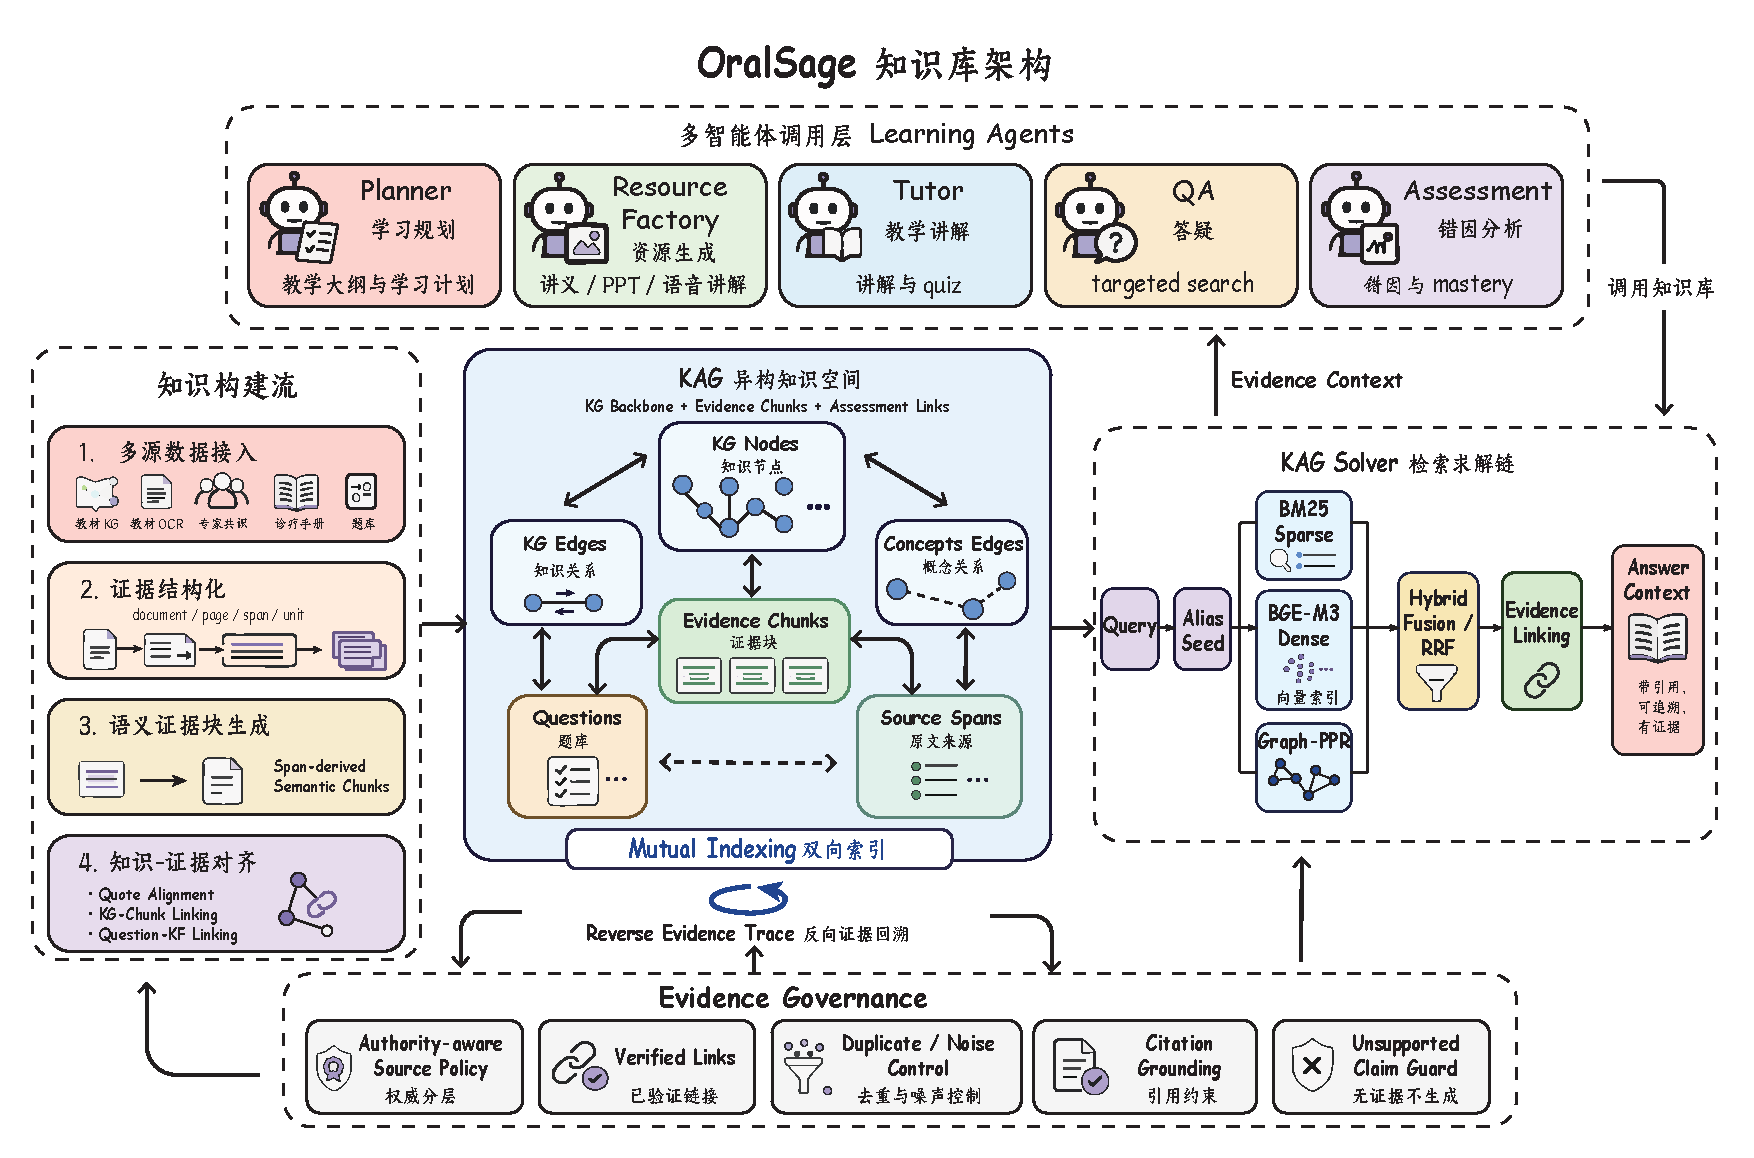
\includegraphics[width=\linewidth]{kb-architecture.pdf}
  \caption{OralSage KAG 知识库总体架构}
  \label{fig:kb-architecture}
\end{figure}

图中左侧构建流对应前述多源资料处理、知识图谱构建和统一入库过程，中央异构知识空间负责保存知识节点、关系、文本单元、来源片段和题目对象。右侧 KAG Solver 将这些对象组织为可检索的知识服务，其召回、图扩展、融合排序和结果补全过程在 6.6 节中展开说明。

底部来源与质量控制贯穿对象构建和在线检索，负责保持知识对象、文本内容与资料位置之间的对应关系；顶部多智能体调用区通过统一接口获取已经组织的检索上下文。由此，本节侧重说明各区域在总体架构中的位置与协作关系，具体算子封装见 6.5 节，检索约束和内容审查见 6.7 节。

\subsection{六层知识服务组织}

最终，本项目知识库组织为六个层次，如图~\ref{fig:kb-layered-architecture} 所示，依次完成资料定位、语义组织、图谱关联和索引生成。

\begin{figure}[H]
  \centering
  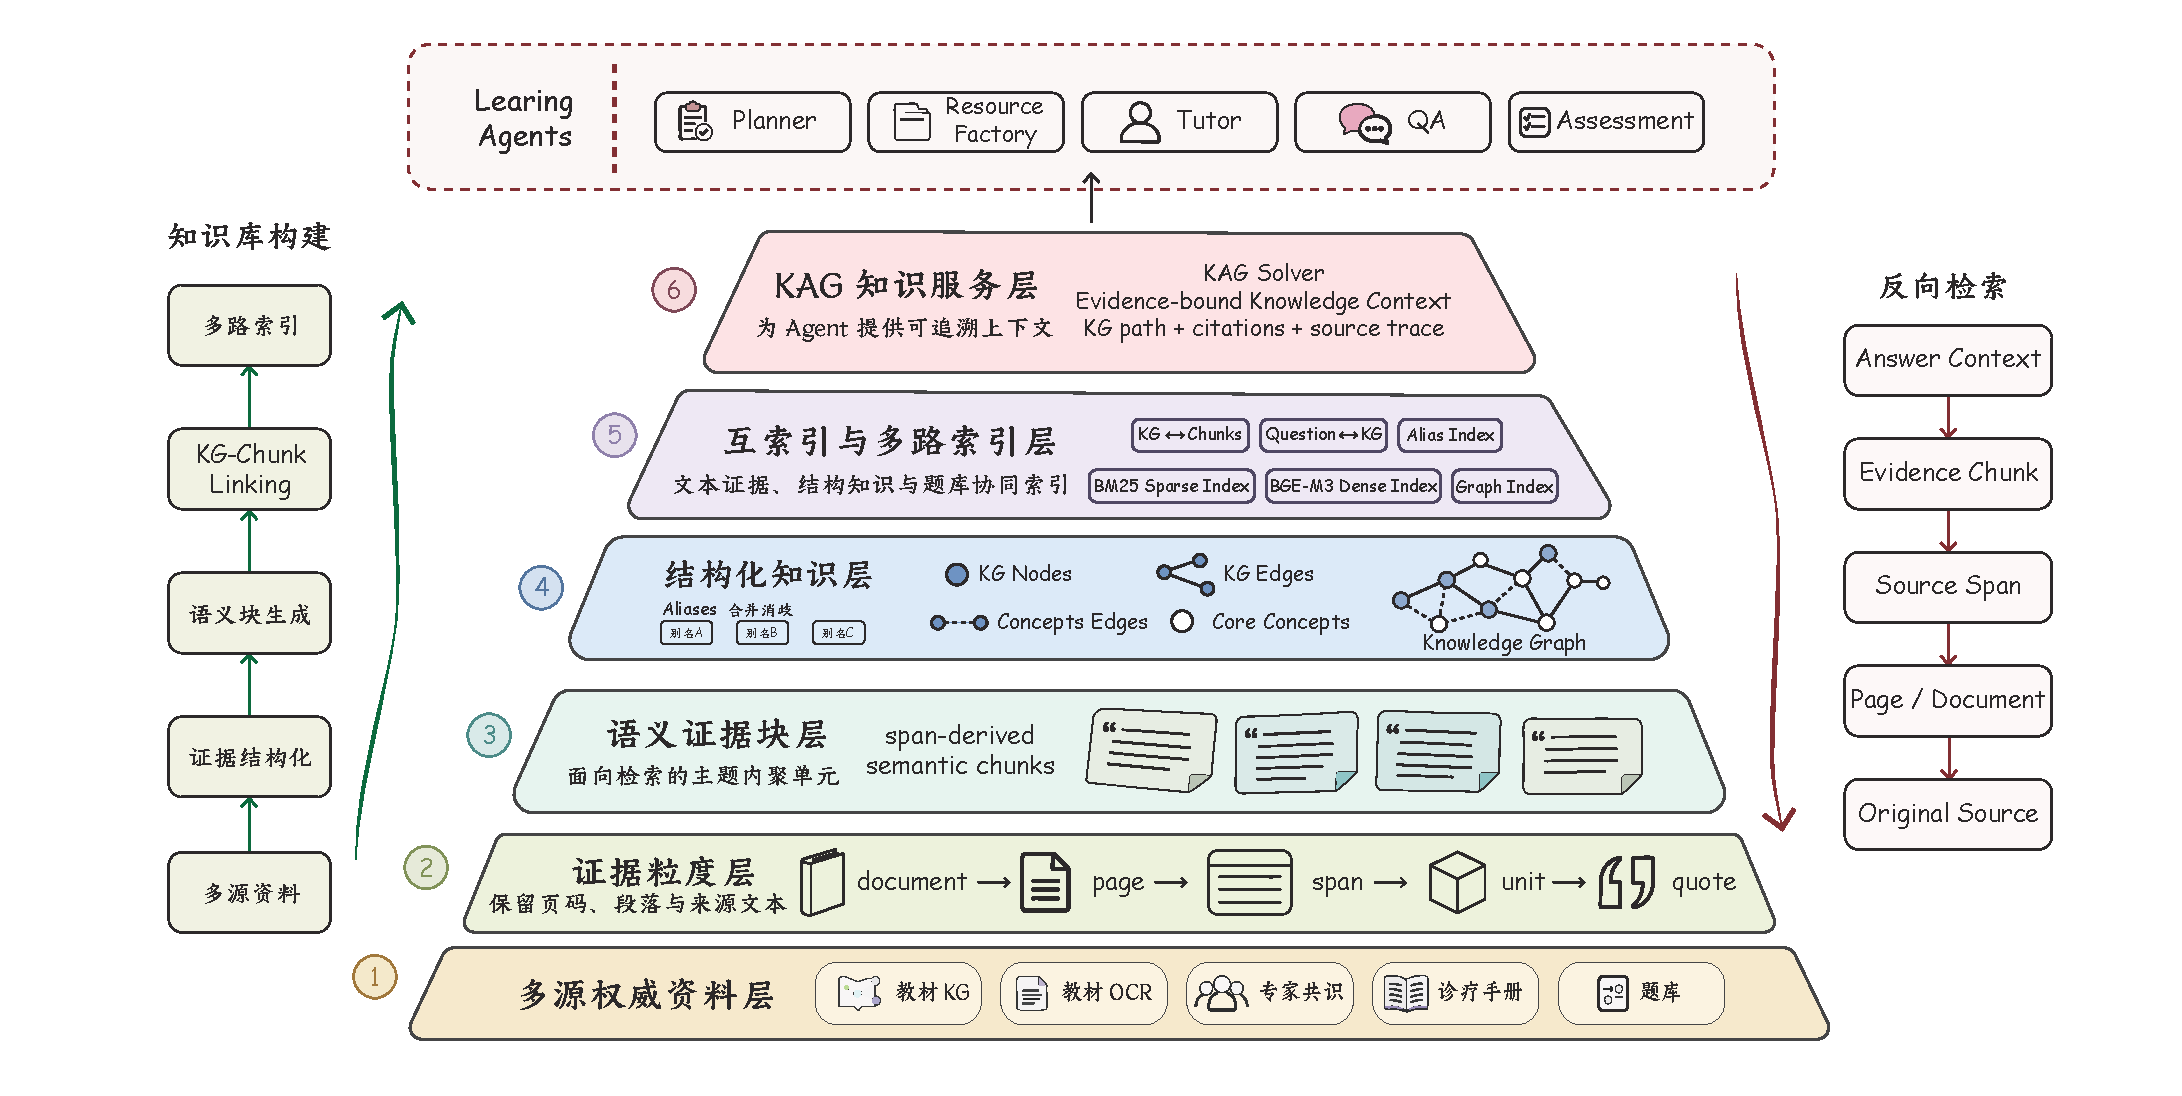
\includegraphics[width=\linewidth]{kb-layered-architecture.pdf}
  \caption{OralSage KAG 知识库分层结构}
  \label{fig:kb-layered-architecture}
\end{figure}


\section{自定义算子设计}

\subsection{算子设计规范}

OralSage 将知识库构建与在线检索拆分为若干具有明确输入和输出的算子。这里的自定义主要体现为对资料对象、知识图谱对象、索引资产和智能体接口进行统一编排，使 KAG 的基础组件能够接入本项目的数据处理流程。各算子沿用统一的对象标识和元数据格式，输入中记录资料类型、来源位置和质量标记，输出中保留对象之间的关联关系。

每个算子采用独立名称标识，并说明所属处理阶段、输入对象和输出对象。离线算子按照确定的顺序生成文本单元、知识对象和索引资产，并将运行结果写入构建清单，便于检查数据是否完整。在线算子以查询和已生成的索引为输入，返回候选内容、知识关系、资料位置和检索记录。

\subsection{数据与索引构建算子}

数据与索引构建算子按照资料规范化、语义单元生成、知识对象关联、索引校验的顺序执行。前两步将不同格式的来源资料转换为可检索的文本单元，第三步连接教材知识图谱、文本和题库，最后一步生成多路索引并检查各类对象之间的对应关系。

\begin{table}[H]
  \centering
  \caption{知识库数据与索引构建算子}
  \label{tab:kb-build-operators}
  \begin{tabularx}{\linewidth}{>{\raggedright\arraybackslash}p{0.24\linewidth}>{\raggedright\arraybackslash}p{0.20\linewidth}X}
    \toprule
    算子名称 & 处理阶段 & 输入与输出 \\ 
    \midrule
    Source Normalizer & 资料规范化 & {输入：} PDF、网页文本、OCR 文本、题库记录和来源信息。\newline {输出：} 文档记录、清理文本、标题路径、资料位置和质量标记。 \\ 
    Span Semantic Chunker & 语义单元生成 & {输入：} 段落单元、标题路径、引文范围和长度参数。\newline {输出：} 按主题边界组织的语义文本单元、来源片段和局部位置。 \\ 
    Canonical Object Builder & 知识对象规范化 & {输入：} 教材知识图谱草稿、题库匹配结果和资料属性。\newline {输出：} 具有统一标识和章节归属的知识节点、知识关系、概念关系、别名和题目对象。 \\ 
    KG--Chunk Linker\newline Question--KG Linker & 对象关联 & {输入：} 知识节点、文本单元、来源片段和题目对象。\newline {输出：} 知识到文本、文本到来源、题目到知识点的链接。 \\ 
    Sparse BM25 Builder\newline Dense BGE-M3 Builder\newline Graph Index Builder & 多路索引生成 & {输入：} 统一检索语料、BGE-M3 模型、知识关系和别名。\newline {输出：} BM25、向量、FAISS、图邻接和别名索引。 \\ 
    Index Asset Validator & 资产校验 & {输入：} 正式对象、索引和构建清单。\newline {输出：} 对象标识、链接目标、文档顺序和向量顺序的校验结果。 \\ 
    \bottomrule
  \end{tabularx}
\end{table}


\subsection{检索与结果组织算子}

在线检索被封装为候选召回、图扩展、候选筛选、融合排序、内容补全和上下文组织等具有明确输入输出的算子，如表~\ref{tab:kb-query-operators}所示。本节侧重说明各算子的职责边界，具体检索公式、参数和执行过程在 6.6 节中展开。

\begin{table}[H]
  \centering
  \caption{KAGSolver 在线检索算子}
  \label{tab:kb-query-operators}
  \begin{tabularx}{\linewidth}{>{\raggedright\arraybackslash}p{0.24\linewidth}>{\raggedright\arraybackslash}p{0.20\linewidth}X}
    \toprule
    算子名称 & 处理阶段 & 输入与输出 \\ 
    \midrule
    Alias Seed\newline Sparse BM25\newline Dense BGE-M3 & 候选召回 & {输入：} 查询、别名索引、BM25 索引和 FAISS 索引。\newline {输出：} 术语命中、关键词重合和近义表达对应的候选集合。 \\ 
    Graph Seed Collector\newline Graph-PPR Expansion & 图种子汇聚与扩展 & {输入：} 多路候选和图邻接。\newline {输出：} 知识节点种子、图候选、局部关联对象和关系路径。 \\ 
    Hybrid Union\newline Quality Gate & 候选合并与筛选 & {输入：} 多路候选、资料属性和质量标记。\newline {输出：} 按统一对象标识合并并完成质量筛选的候选集合。 \\ 
    RRF Fusion & 融合排序 & {输入：} 各通道排名和候选顺序。\newline {输出：} RRF 排序结果与融合分数。 \\ 
    Evidence Hydration\newline Citation Builder\newline KG Path Builder & 内容与路径补全 & {输入：} 排序后的对象标识、知识关系和来源位置。\newline {输出：} 智能体可读的完整文本、知识节点、关系路径和引用位置。 \\ 
    Agent Payload Builder & 上下文组织 & {输入：} 补全后的对象、排序信息和检索记录。\newline {输出：} 面向 Planner、Resource Factory、Tutor、QA 和 Assessment 的统一检索上下文与检索轨迹。 \\ 
    \bottomrule
  \end{tabularx}
\end{table}

算子之间通过统一的对象标识传递结果，保留参与的召回通道、候选数量、图扩展结果、排序方式和资料位置，便于分析一次检索由哪些步骤产生，集中处理检索和结果组织。

\section{知识库检索}

\begin{figure}[H]
  \centering
  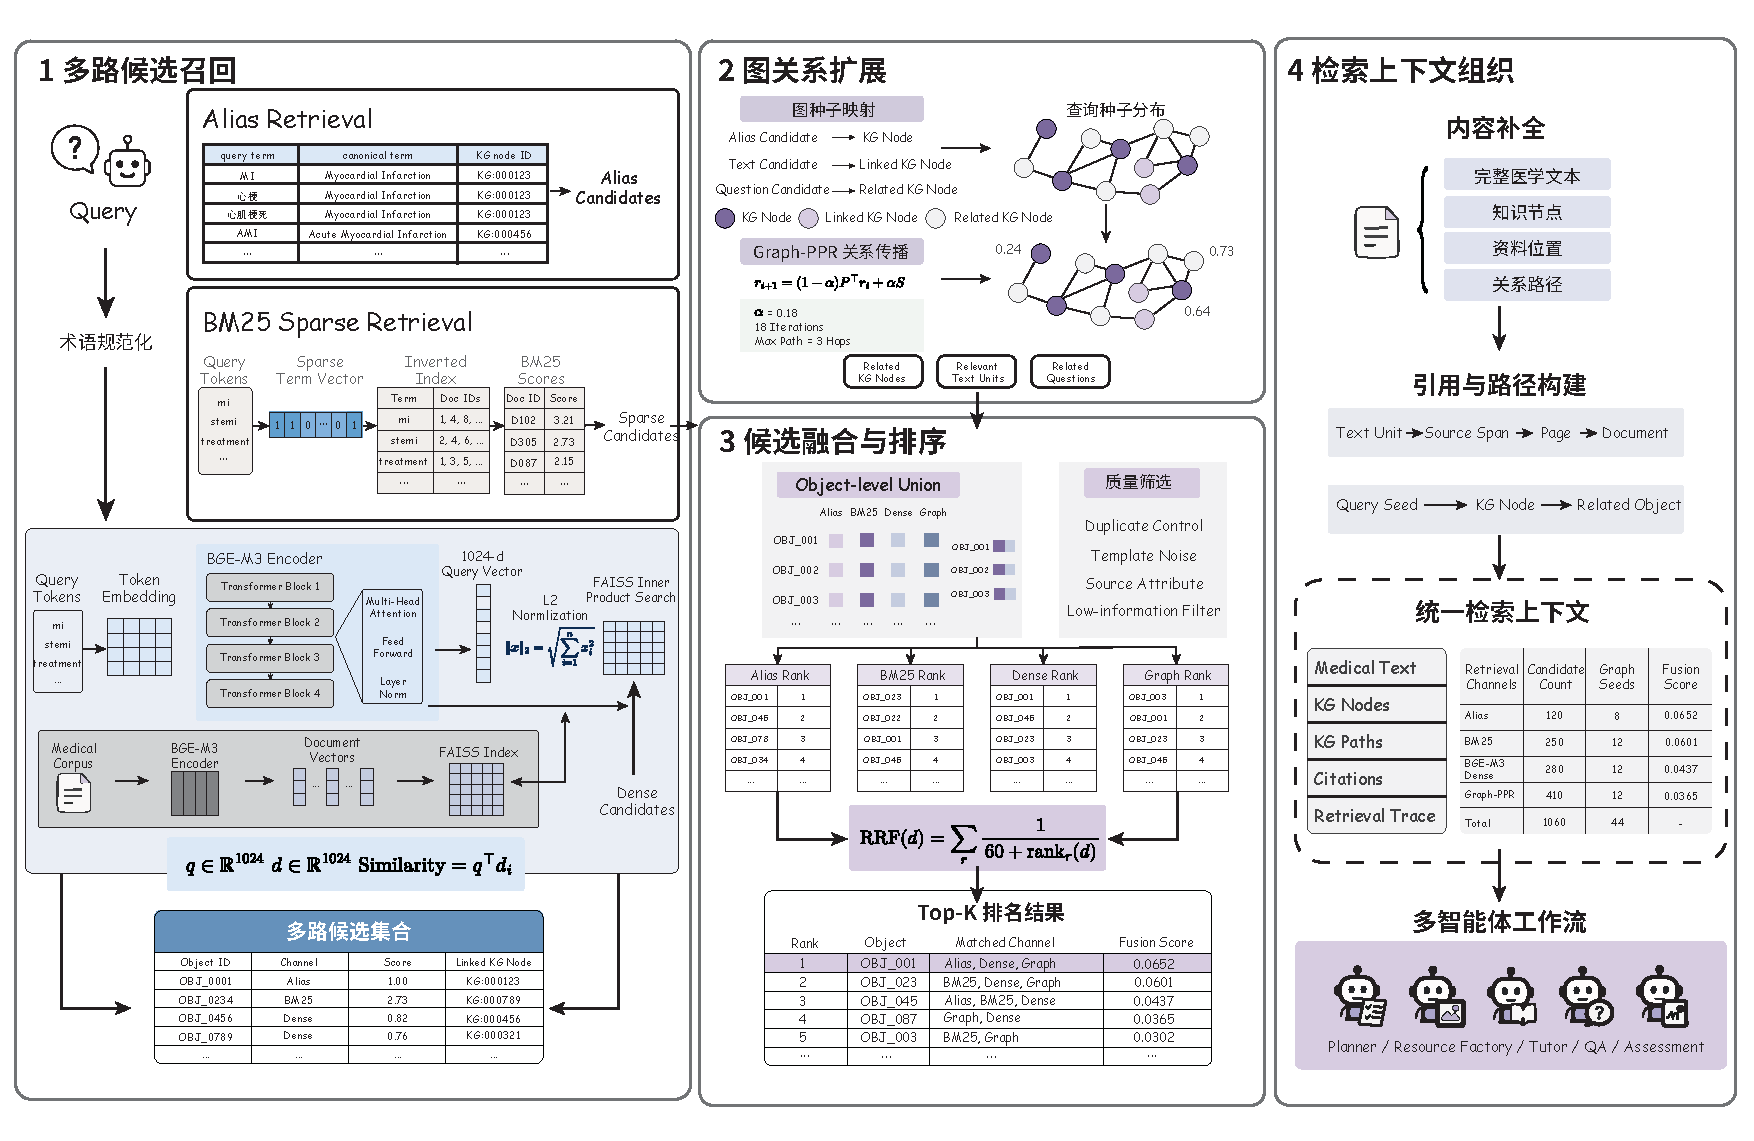
\includegraphics[width=\linewidth]{kb-search-process.pdf}
  \caption{OralSage 知识库检索流程}
  \label{fig:kb-search-process}
\end{figure}

知识库检索按照图~\ref{fig:kb-search-process} 所示的四个阶段执行。查询经过术语规范化后进入 Alias、BM25 和 BGE-M3 三路召回，各通道返回的候选映射到知识节点，并由 Graph-PPR 沿局部关系扩展相关节点、医学文本和题目。多路结果按照统一对象标识合并，经过质量筛选和 RRF 排序后补充完整医学文本、知识节点、资料位置、关系路径与引用信息，最终形成供 Planner、Resource Factory、Tutor、QA 和 Assessment 调用的统一检索上下文。


\subsection{多路候选召回}

KAGSolver 并行执行术语别名、BM25 和 BGE-M3 三路召回。术语别名通道直接匹配知识节点名称、别名和缩写，适合识别规范疾病名称、检查术语和治疗名称。BM25 通道对中英文内容进行词项切分，并保留医学术语、数字、英文缩写和教材表述之间的精确重合，适合处理定义查询和条件明确的问题。BGE-M3 通道对查询与检索文本进行语义编码，用于发现表达方式不同但医学含义接近的内容。

BM25 使用平滑后的逆文档频率衡量词项区分度。设语料库文档总数为 \(N\)，包含词项 \(t\) 的文档数为 \(df(t)\)，则：

\begin{equation}
  \label{eq:bm25-idf}
  \operatorname{idf}(t)=\log\left(\frac{N-df(t)+0.5}{df(t)+0.5}+1\right)
\end{equation}

对于查询 \(q\) 和文档 \(d\)，BM25 文档得分表示为：

\begin{equation}
  \label{eq:bm25-score}
  \operatorname{Score}_{\mathrm{BM25}}(q,d)
  =\sum_{t\in q}qtf(t)\operatorname{idf}(t)
  \frac{tf(t,d)(k_1+1)}
  {tf(t,d)+k_1\left(1-b+b\frac{|d|}{\operatorname{avgdl}}\right)}
\end{equation}

式中，\(tf(t,d)\) 和 \(qtf(t)\) 分别表示词项在文档和查询中的出现次数，\(|d|\) 表示文档长度，\(\operatorname{avgdl}\) 表示平均文档长度。系统设置 \(k_1=1.5\)、\(b=0.75\)。

BGE-M3 的最大输入长度为 512 个词元，编码后得到 1,024 维向量。设 \(E(x)\) 为文本 \(x\) 的编码结果，向量归一化与语义相关度计算为：

\begin{equation}
  \label{eq:dense-score}
  \hat{E}(x)=\frac{E(x)}{\lVert E(x)\rVert_2},
  \qquad
  \operatorname{Score}_{\mathrm{dense}}(q,d)=\hat{E}(q)^{\top}\hat{E}(d)
\end{equation}

归一化后的内积等价于余弦相似度，FAISS 据此返回语义距离较近的文本。三路召回结果保留各自的匹配方式和排名信息，为图关系扩展与融合排序提供输入。

\subsection{图种子汇聚与 Graph-PPR}

图种子汇聚模块将三路召回结果转换为知识节点。术语别名命中的节点直接加入种子集合，BM25 或 BGE-M3 命中知识节点时使用对应节点标识，命中文本单元或题目时则沿对象链接取得相关知识点。由此，名称匹配、词项匹配和语义匹配均能进入同一图扩展过程。

Graph-PPR 采用 Personalized PageRank 的局部随机游走思想\cite{page1999pagerank}。设 \(S\) 为查询种子分布，\(P\) 为图转移矩阵，\(\alpha\) 为重启概率，则迭代过程为：

\begin{equation}
  \label{eq:graph-ppr}
  r_{t+1}=(1-\alpha)P^{\top}r_t+\alpha S
\end{equation}

系统设置 \(\alpha=0.18\)，执行 18 次迭代，并从节点关系、概念关系、知识到文本关系和题目到知识点关系中取得局部候选。关系路径保留查询种子到结果对象的三跳以内连接，用于说明内容之间的知识联系。

\subsection{候选融合与 RRF 排序}

术语别名、BM25、BGE-M3 和 Graph-PPR 返回的候选按照统一对象标识合并，相同对象只保留一条记录，同时汇总其匹配通道和图关系得分。候选筛选读取资料属性与质量标记，降低重复文本、模板内容和参考文献密集片段的排序优先级。完成合并与筛选后，系统使用倒数排名融合方法计算综合顺序\cite{cormack2009rrf}：

\begin{equation}
  \label{eq:rrf}
  \operatorname{Score}_{\mathrm{RRF}}(d)=\sum_{r\in R_d}\frac{1}{k+\operatorname{rank}_r(d)}
\end{equation}

其中，\(R_d\) 表示对象 \(d\) 进入的排名通道集合，\(\operatorname{rank}_r(d)\) 表示该对象在通道 \(r\) 中的名次，平滑常数 \(k\) 取 60。一个对象由多个通道共同召回时，其综合得分会相应提高，从而兼顾精确术语命中、语义相关性和图关系关联。

\subsection{检索结果组织}

排序完成后，KAGSolver 根据对象标识读取完整内容，并组织为医学文本、相关知识节点、关系路径、引用位置和检索轨迹。医学文本保留资料类型、标题路径和来源片段，引用位置记录资料名称、页码范围及局部片段，关系路径记录查询种子到结果对象之间的连接。检索轨迹则汇总参与的召回通道、候选数量、图种子数量和融合分数。

这些内容采用统一结构返回，使上层调用既能取得直接用于生成的医学文本，也能读取与其关联的知识点和资料位置。结果组织阶段按照返回数量控制上下文规模，并保留排序分数和匹配方式，便于不同学习任务选择合适内容。

\subsection{KAGSolver 与智能体调用}

后端将 KAGSolver 作为进程内单例使用，首次调用加载检索语料、BM25、FAISS、图邻接、别名索引和 BGE-M3 查询编码器，后续请求复用已加载的索引与模型。统一检索接口将 KAG 返回结果映射为 \texttt{EvidenceChunk} 对象，使各智能体使用一致的文本、来源和分数格式。

Planner 在课程规划前检索主题相关知识，并结合章节归属和关系路径确定学习范围。Resource Factory 根据讲义小节组织定向查询，Tutor 与 QA 调用医学文本和引用位置完成讲解与答疑，Assessment 通过题目到知识点的关系分析错因并更新掌握情况。各智能体可以改变查询内容和返回数量，同时复用同一套检索链路与结果结构。

\section{防幻觉与内容审查机制}

口腔医学学习内容包含疾病定义、诊断条件、治疗原则、用药说明和操作要求，术语、数值或适用条件发生偏移都会改变医学含义。OralSage 将检查环节安排在输入接收、资料检索、上下文构造、内容生成和结果输出五个阶段，使用户请求、检索材料、生成陈述与引用位置保持明确对应。

\subsection{多阶段医学内容处理}

资料进入知识库时已进行 PDF 版面和网页层级恢复，清理 OCR 异常、重复页眉、模板文本及参考文献密集片段，并保留文档、页面、片段和标题路径。重复文本、免责声明和低信息内容写入质量标记，知识节点与文本之间的链接经过标识、目标和位置检查后参与检索。由此，模型接收的医学内容已经完成基础清理，并保留能够定位到具体资料的来源信息。不同资料按照内容类型进入生成过程。系统优先采用临床规范与教材中的明确结论，同时保留资料类型，使通用医学参考和考试材料在各自范围内参与内容组织。

在线检索阶段由 Quality Gate 读取来源属性与质量标记，过滤模板化内容，降低重复文本和参考文献密集片段的排序优先级。Alias、BM25、BGE-M3 和 Graph-PPR 返回的候选按照统一对象标识合并，再由 RRF 形成综合顺序。多路结果共同进入排序，可以减少单一关键词相似或单一语义相似带来的偏差。

\subsection{检索约束和引用绑定}

KAGSolver 将医学文本、知识节点、关系路径、资料位置和检索记录进行上下文统一，并要求医学陈述使用上下文中的材料，限制自行补充外部知识，并对药物剂量、诊断阈值、禁忌证、操作条件和疾病分类采用关键术语保留策略。

引用信息按照以下位置链组织，使生成内容能够定位到具体资料：

\begin{center}
  \softid{智能体上下文 -> 检索文本单元 -> 来源片段 -> 页面 -> 资料}
\end{center}

Citation Builder 为返回内容补充资料标题、页码范围和局部片段，KG Path Builder 记录查询种子与相关知识对象之间的关系路径，Retrieval Trace 保存召回通道、候选数量和融合顺序。通过引用绑定，使回答中的医学陈述与相应文本位置一并输出，并为后续审查提供可核对的内容单元\cite{mirage2024}。

Resource Factory 在生成讲义前先从检索结果中选择本节所需的知识节点、知识关系、题目和文本单元，再执行定向检索补充材料。内容生成完成后，程序核对实际使用的对象标识是否属于本次检索允许集合，定向检索获得的文本按照文本单元参与引用，知识节点和关系则保持知识库中已有的对象类型，从而避免生成过程自行构造不存在的知识对象或资料位置。

\subsection{输出过滤与分级审查}

输出审查首先检查结构完整性。后端依据预定义数据结构核对字段类型、必填内容、文本长度和对象标识，无法解析的结构不会进入资源派生与页面展示。对于带有医学陈述的讲义和回答，程序继续检查引用标识是否存在、引用位置是否属于相应资料，以及生成结果使用的知识节点、关系和题目是否来自本次允许集合。

系统重点核对疾病名称、分型、药物剂量、诊断阈值、适应证、禁忌证和操作条件。一般讲解内容检查陈述与引用文本的语义对应，包含数值和临床条件的内容还需比对关键术语与数值。对于需要细粒度复核的回答，审查程序将回答拆分为独立医学陈述，并使用 BGE Reranker 计算陈述与检索材料的对应分数，随后标记需要重新检索或改写的内容，保证医学一致性。

内容安全检查面向个体化诊断、处方剂量、侵入性操作、自伤伤人、药物滥用和其他可能造成现实伤害的输出。检测到高风险内容后，系统移除可直接执行的步骤、剂量和操作细节，将回答转换为医学常识、风险提示、就医建议或紧急求助指引。面向课程学习的定义、机理和规范性知识继续保留，输出范围限定在教学解释和经过引用的医学材料内。

\subsection{有害输入识别}

当输入包含要求忽略既有规则、泄露系统提示词、伪造引用、虚构资料位置或改变智能体职责的指令时，处理程序保留其中可识别的学习主题，阻断其控制意图。检索获得的网页文字和题库文本同样按医学材料处理，其中出现的命令式语句不会替代系统指令。

输入审查将请求区分为正常学习、医学高风险、指令操纵和有害行为等类型。涉及自伤伤人、毒物使用、处方药滥用、危险器械操作或规避医疗监管的请求进入安全响应流程，系统不提供可执行步骤、精确剂量和规避方法，转而给出风险说明、专业医疗建议和紧急求助信息。经过拆字、编码、同义替换或多轮诱导重复提交的请求仍按规范化后的语义进行判断，保持输入处理规则的一致性。

\chapter{系统实现}
\label{sec:implementation}

\section{技术栈}

\begin{table}[H]
  \centering
  \caption{技术栈说明}
  \label{tab:tech-stack-implementation}
  \begin{tabularx}{\linewidth}{p{0.20\linewidth}p{0.24\linewidth}X}
    \toprule
    层次 & 技术或组件 & 说明 \\
    \midrule
    前端 & HTML/CSS/JavaScript & 实现学习入口、画像、学习页、资源展示和计划页等。 \\
    后端 & Python、FastAPI、Pydantic、Uvicorn & 提供 API、参数校验、静态资源和流式进度接口。 \\
    智能体 & Orchestrator、Planner、Resource Factory、Tutor、QA、Assessment、Memory/User Model & 实现学习规划、资源生成、答疑、测评和记忆更新。 \\
    临床训练 & 患者 Agent、判官 Agent、状态机、数字人 SDK & 支持数字人问诊、自然语言诊断理解、五域表达考核和画像反馈。 \\
    知识库 & KAG、KG、题库、BM25、BGE-M3/FAISS & 支撑证据检索、路径规划和测评。 \\
    多模态资源 & PPT/slides、TTS 音频、思维导图、阶段卷 & 支撑多类型个性化学习资源生成。 \\
    \bottomrule
  \end{tabularx}
\end{table}

\section{讯飞平台与 API 集成}

作品的开发工具和运行时服务分别采用讯飞平台中的不同产品。开发阶段使用讯飞官方的 \textbf{iFlyCode 智能编程助手}，用于代码生成、代码续写、代码检查、单元测试和调试辅助；iFlyCode 只参与项目开发过程，不作为用户请求处理时的运行时依赖。

系统运行时的文本智能体统一接入讯飞星火 4.0 Ultra API，用于课程规划、讲义生成、Tutor 讲解、即时答疑、学习测评和学习状态分析。该接口采用 OpenAI 兼容的 HTTP 调用方式，后端通过统一的模型客户端读取 Base URL、模型名称和服务端密钥，各 Agent 不直接依赖具体模型厂商的请求格式。部署配置如下：

\begin{lstlisting}
LEARNING_LLM_BASE_URL=https://spark-api-open.xf-yun.com/v1
LEARNING_LLM_MODEL=4.0Ultra
LEARNING_LLM_API_KEY=<APIPassword>
\end{lstlisting}

数字问诊使用讯飞星火 \texttt{xsparkx2flash} 推理服务处理病例选题映射、患者多轮交流、自然语言诊断识别、考核题目构建与分项评分。临床训练服务通过专用配置连接推理接口，并要求模型名称与 \texttt{xsparkx2flash} 一致。结构化输出经过字段、事实编号与证据引用检查后进入状态机，使讯飞星火的中文语义理解能够可靠承接患者和判官两个角色。

语音输入采用讯飞流式语音听写 WebSocket，后端生成短时签名地址供浏览器建立会话，访问密钥始终保留在服务端。听写结果经过医学术语整理后提交给患者 Agent，口腔疾病名称和临床专有词能够以更适合后续推理的文本形式进入问诊。数字人部分使用讯飞实时互动 SDK 和 \texttt{xrtc} 协议，透明渲染层展示患者形象，Agent 回复通过 \texttt{x4\_lingxiaoqi\_oral} 发音人播报，形成语音输入、语义理解和患者表达连续衔接的交互体验。

课程讲稿和 Tutor 内容的语音资源采用讯飞长文本语音合成 API。后端先调用 \texttt{dts\_create} 创建合成任务，再通过 \texttt{dts\_query} 查询任务状态并下载生成的音频文件。部署版本使用中文发音人 \texttt{x4\_mingge}，输出 MP3 音频，服务端保存音频文件并向前端返回资源路径。该方式适合课程讲义和连续讲解等较长文本，不在浏览器端直接保存或暴露讯飞鉴权信息。

\begin{table}[H]
  \centering
  \caption{讯飞平台组件与项目使用位置}
  \label{tab:xfyun-integration}
  \begin{tabularx}{\linewidth}{p{0.25\linewidth}p{0.30\linewidth}X}
    \toprule
    平台组件 & 使用阶段或接口 & 项目中的使用位置 \\
    \midrule
    iFlyCode 智能编程助手 & 开发辅助工具 & 代码生成、代码检查、单元测试和调试，不参与运行时请求 \\
    星火 4.0 Ultra API & \texttt{/v1/chat/completions} & Planner、Resource Factory、Tutor、QA、Assessment 和学习状态分析 \\
    星火 \texttt{xsparkx2flash} & 推理服务 HTTP 接口 & 数字问诊选题、患者交互、诊断理解、判官出题与评分，以及综合考试的简答题命题与评阅 \\
    流式语音听写 & \texttt{/v2/iat} WebSocket & 实时转写学生口述并衔接医学术语整理 \\
    实时数字人 & 实时互动 WebSocket 与浏览器 SDK & 展示并播报患者和判官回复 \\
    长文本语音合成 API & \texttt{dts\_create}/\texttt{dts\_query} & 将课程讲稿和 Tutor 内容生成 MP3 音频 \\
    \bottomrule
  \end{tabularx}
\end{table}

讯飞 API 的 AppID、APIKey、APISecret 和 APIPassword 只在服务端环境变量中配置，不写入源代码、前端静态文件或提交文档。项目保留统一的服务适配层，使模型服务切换不会改变课程规划、资源生成和学习状态模块的数据结构。

\section{后端接口设计}

OralSage 后端基于 FastAPI 构建，围绕学习测评、课程会话、教学互动、学习画像、学习计划和多模态资源等业务域组织接口。后端使用 Pydantic 模型定义请求字段并完成参数校验，使用户标识、学习主题、会话状态、测评答案和计划任务等数据能够按照统一结构进入相应业务模块。

系统根据任务执行特点提供普通请求和流式请求两类接口。画像查询、计划管理和资源状态查询等操作采用普通 HTTP 接口，以 JSON 格式返回处理结果；主题课程启动、课程内答疑和继续学习等耗时操作同时提供基于 Server-Sent Events（SSE）的流式接口，使前端能够持续展示请求接收、智能体调度、资源生成和执行完成等阶段状态。核心接口如表~\ref{tab:core-backend-api} 所示。

{\small
\renewcommand{\arraystretch}{1.12}
\begin{longtable}{
  p{0.14\linewidth}
  p{0.31\linewidth}
  p{0.23\linewidth}
  p{0.23\linewidth}
}
  \caption{OralSage 后端核心接口}
  \label{tab:core-backend-api}\\
  \toprule
  功能 & 方法与路径 & 主要请求参数 & 主要返回内容 \\
  \midrule
  \endfirsthead

  \multicolumn{4}{c}{续表~\thetable}\\
  \toprule
  功能 & 方法与路径 & 主要请求参数 & 主要返回内容 \\
  \midrule
  \endhead

  \bottomrule
  \endfoot

  系统健康检查
  & \texttt{GET /api/system/health}
  & 无
  & 系统运行状态、工作模式和状态说明 \\

  获取初始测评
  & \texttt{GET /api/learning/assessment}
  & 无
  & 测评题目、选项和测评版本 \\

  提交初始测评
  & \texttt{POST /api/learning/assessment/submit}
  & \texttt{user\_id}、测评答案、目标考试和跳过状态
  & 初始学习画像和测评状态 \\

  启动主题学习
  & \texttt{POST /api/learning/session/start}
  & 用户标识、学习主题、显示名称和初始画像信息
  & 新建学习会话及课程启动结果 \\

  流式启动学习
  & \texttt{POST /api/learning/session/start/stream}
  & 与主题学习启动接口一致
  & 知识检索、课程规划和资源准备的 SSE 事件 \\

  查询会话状态
  & \texttt{GET /api/learning/session/\{session\_id\}/state}
  & 路径参数 \texttt{session\_id}
  & 当前策略状态和学习会话摘要 \\

  课程内提问
  & \texttt{POST /api/learning/interruption}
  & 会话标识、用户问题和调度策略选项
  & QA 调度决策、回答结果和更新后的会话状态 \\

  继续课程学习
  & \texttt{POST /api/learning/continue}
  & 会话标识和调度策略选项
  & 下一阶段调度决策、Tutor 执行结果和会话状态 \\

  提交随堂答案
  & \texttt{POST /api/learning/answer}
  & 会话标识、题目信息和用户答案
  & Assessment 执行结果、答题反馈和状态更新 \\

  获取与生成阶段卷
  & \texttt{GET/POST /api/learning/session/\{session\_id\}/stage-exam}
  & 会话标识、是否重新生成和每节题目数量
  & 阶段试卷内容及当前测评状态 \\

  提交阶段卷
  & \texttt{POST /api/learning/session/\{session\_id\}/stage-exam/submit}
  & 题目标识和所选答案列表
  & 得分、题目解析、薄弱内容和测评结果 \\

  生成综合考试试卷
  & \texttt{POST /api/learning/comprehensive-exams}
  & \texttt{user\_id}
  & 考试标识、十五道单选题、五道简答题和试卷摘要 \\

  提交综合考试
  & \texttt{POST /api/learning/comprehensive-exams/\{exam\_id\}/submit}
  & 用户标识和全部题目作答
  & 总分、单选与简答分项得分、逐题反馈、参考答案和解析 \\

  查询学习画像
  & \texttt{GET /api/learning/profile/\{user\_id\}}
  & 路径参数 \texttt{user\_id}
  & 基础画像、长期记忆、学习摘要和近期事件 \\

  获取画像切片
  & \texttt{POST /api/learning/profile/slice}
  & 用户标识、Agent 角色、任务上下文和数量限制
  & 面向当前 Agent 的学习画像子集 \\

  推荐学习计划
  & \texttt{POST /api/learning/plan/recommend}
  & 用户标识、计划日期、任务数量和自然语言需求
  & 指定日期的学习计划推荐草案 \\

  查询学习计划
  & \texttt{GET /api/learning/plan/\{user\_id\}/month}
  & 年份和月份
  & 按日期组织的月度学习任务 \\

  管理计划任务
  & \texttt{POST/DELETE /api/learning/plan/items}
  & 日期、标题、任务类型、课程和知识节点信息
  & 创建、修改、完成、延期或删除后的任务状态 \\

  获取课程资源
  & \texttt{GET /api/learning/session/\{session\_id\}/slides}
  & 会话标识
  & 当前课程的结构化课件数据 \\

  获取课件预览
  & \texttt{GET /api/learning/session/\{session\_id\}/ppt-preview}
  & 会话标识
  & 课件页面信息和预览图片地址 \\

  下载 PPT 文件
  & \texttt{GET /api/learning/session/\{session\_id\}/pptx}
  & 会话标识
  & 当前课程生成的 PPTX 文件 \\

  获取语音资源
  & \texttt{GET /api/learning/session/\{session\_id\}/audio-manifest}
  & 会话标识
  & 分节语音资源及其文件清单 \\

  数字问诊就绪检查
  & \texttt{GET /api/clinical-speaking/readiness}
  & 无
  & 星火、语音听写、数字人和病例训练条件 \\

  数字问诊会话
  & \texttt{GET/POST /api/clinical-speaking/sessions}
  & 用户标识、请求编号
  & 历史会话列表或新建的个性化病例会话 \\

  提交问诊轮次
  & \texttt{POST /api/clinical-speaking/sessions/\{session\_id\}/turns}
  & 用户文本、输入方式、请求编号
  & 患者回复、意图理解和当前阶段 \\

  确认诊断
  & \texttt{POST /api/clinical-speaking/sessions/\{session\_id\}/diagnosis}
  & 诊断确认、请求编号
  & 判官接管结果和首道考核问题 \\

  提交考核回答
  & \texttt{POST /api/clinical-speaking/sessions/\{session\_id\}/exam-answers}
  & 问题编号、回答文本、请求编号
  & 分项分数、批评意见、下一问题或训练总结 \\

  获取语音听写配置
  & \texttt{GET /api/clinical-speaking/iat-config}
  & 无
  & 短时签名地址和公开听写参数 \\
  \end{longtable}
}

普通接口采用统一的 JSON 响应结构。响应中的 \texttt{ok} 表示本次调用是否成功，\texttt{module} 标识所属业务模块，\texttt{action} 表示实际执行动作，\texttt{result} 保存学习会话、课程资源、画像或计划任务等业务数据。以主题学习启动接口为例，其基础响应结构如下：

\begin{lstlisting}
{
  "ok": true,
  "module": "learning",
  "action": "start_lesson",
  "result": {
    "...": "课程启动与会话结果"
  }
}
\end{lstlisting}

流式接口使用 \texttt{text/event-stream} 返回执行过程。事件主要包括 \texttt{start}、\texttt{progress}、\texttt{complete} 和 \texttt{error}。其中，开始事件用于确认请求已经进入系统，进度事件用于提示当前正在进行知识检索、课程规划或智能体执行，完成事件返回最终业务结果，错误事件则记录发生异常的阶段和错误信息。该机制使前端在等待课程与资源生成时仍能展示明确的执行进度。

后端同时根据错误类型返回相应的 HTTP 状态码，主要错误处理规则如表~\ref{tab:backend-error-codes} 所示。

\begin{table}[H]
  \centering
  \caption{后端接口主要错误状态}
  \label{tab:backend-error-codes}
  \begin{tabularx}{\linewidth}{p{0.16\linewidth}p{0.27\linewidth}X}
    \toprule
    状态码 & 错误类型 & 典型情况 \\
    \midrule
    400 & 请求内容无效
        & 测评答案、计划日期或阶段卷提交内容不符合业务要求 \\
    401/403 & 身份或权限异常
        & 用户未登录、微信内部认证失败或跨用户读取计划草案 \\
    404 & 对象或资源不存在
        & 学习会话、计划任务、音频、课件或阶段卷不存在 \\
    409/410 & 资源状态冲突
        & PPTX 尚未生成、阶段卷当前不可用或计划草案已经过期 \\
    422 & 请求字段校验失败
        & 缺少必填字段、字段类型错误或参数范围不符合模型约束 \\
    500/503 & 内部或外部服务异常
        & 资源文件无法解析、内部执行失败或外部服务暂时不可用 \\
    \bottomrule
  \end{tabularx}
\end{table}

通过上述接口，前端可以围绕同一用户和学习会话依次完成初始测评、主题课程启动、讲解与答疑、练习测评、画像更新、计划推荐和多模态资源获取。数字问诊接口另行维护患者会话和临床考核状态，并把诊断与评分事件写入同一学习画像。两类学习过程共享用户身份和专业知识空间，页面可以呈现连续积累的个人学习变化。

\section{前端页面设计}

OralSage 前端采用统一导航组织核心学习页面，顺序为总控学习入口、智能问答、问诊模拟、学习计划、学习画像和知识图谱。首页保留智能问答、问诊模拟、综合考试、知识图谱、学习画像、学习计划和专业工具等主要入口，知识库查看移入工具箱并以独立页面打开。主题学习、学习计划生成和课程交互仍从总控对话页面进入，数字问诊拥有单独页面，使实时数字人、历史会话与连续问诊获得更完整的展示空间。

综合考试页面采用“生成试卷、开启摄像头、开始考试、提交评卷”的顺序组织交互。试卷生成完成后，页面请求摄像头权限并显示本地预览。计时开始后，单选题与简答题分别显示在答题卡中，学习者可在二十道题目之间切换。交卷请求返回后，结果页展示单选题解析，并将讯飞星火对简答题给出的得分、反馈、参考答案、评分要点和证据解析集中呈现。页面通过不同深浅的淡紫色区分满分题目与仍有可补充内容的题目，帮助学习者快速定位需要回看的作答。

\begin{figure}[H]
  \centering
  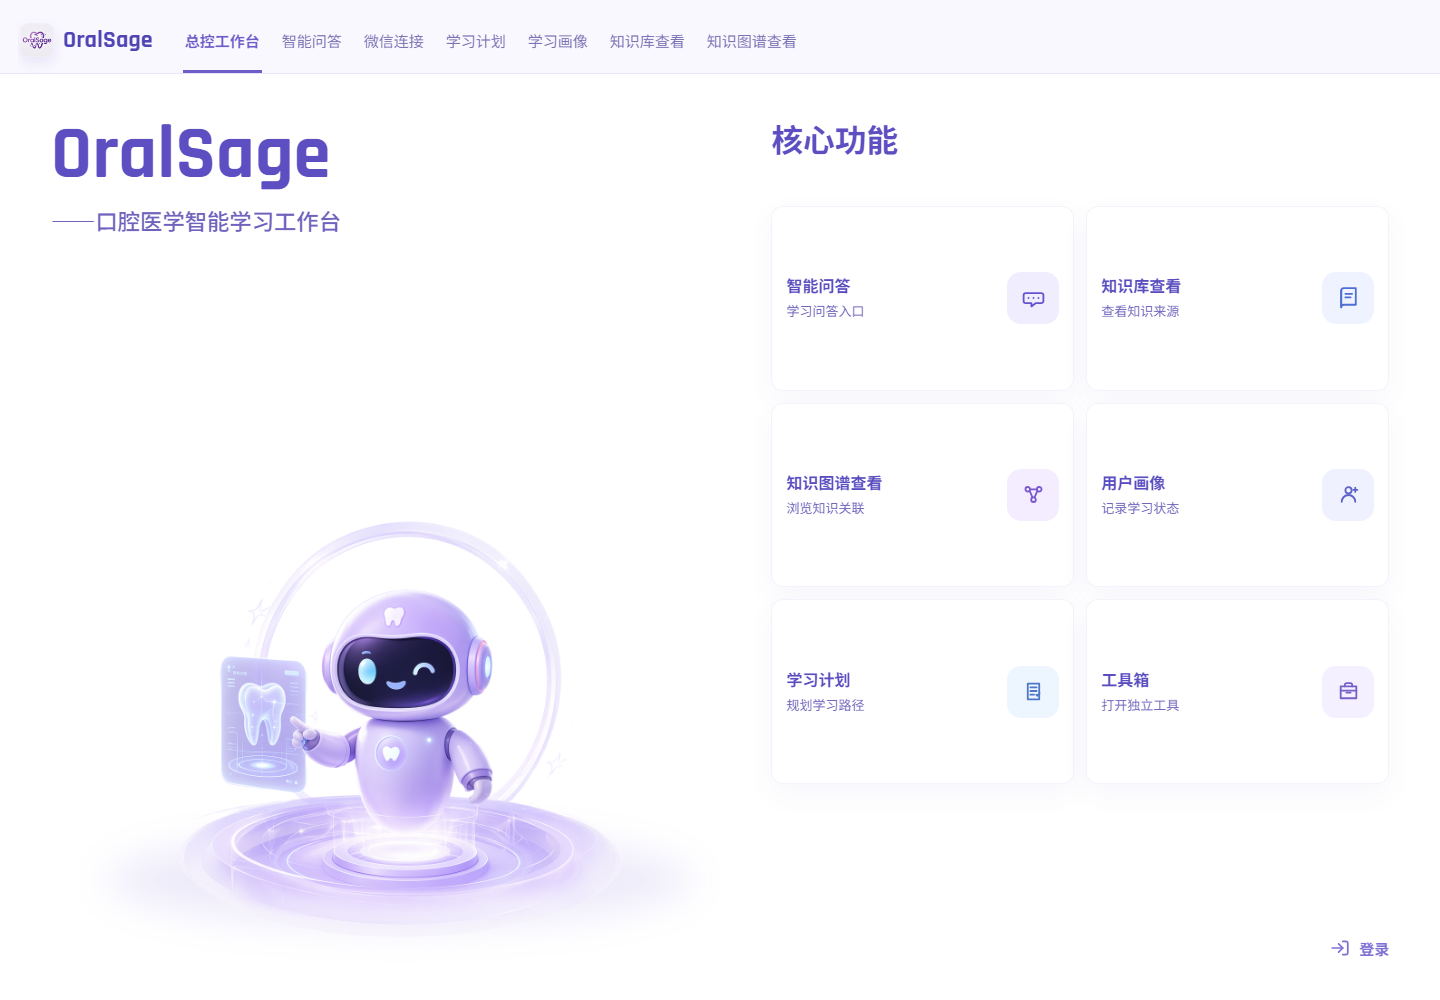
\includegraphics[width=0.92\linewidth]{ui-home.png}
  \caption{OralSage 首页与核心功能入口}
  \label{fig:ui-home}
\end{figure}

在主题学习场景中，学习者可以直接输入希望学习的口腔医学主题，由系统组织课程内容并进入连续讲解。以“系统学习牙周炎”为例，页面在同一会话中呈现当前学习单元和讲解内容，并提供继续下一节、针对本节提问、本节自测和同步演示等后续操作，使课程讲解、即时答疑与理解检验形成连续的学习过程。

\begin{figure}[H]
  \centering
  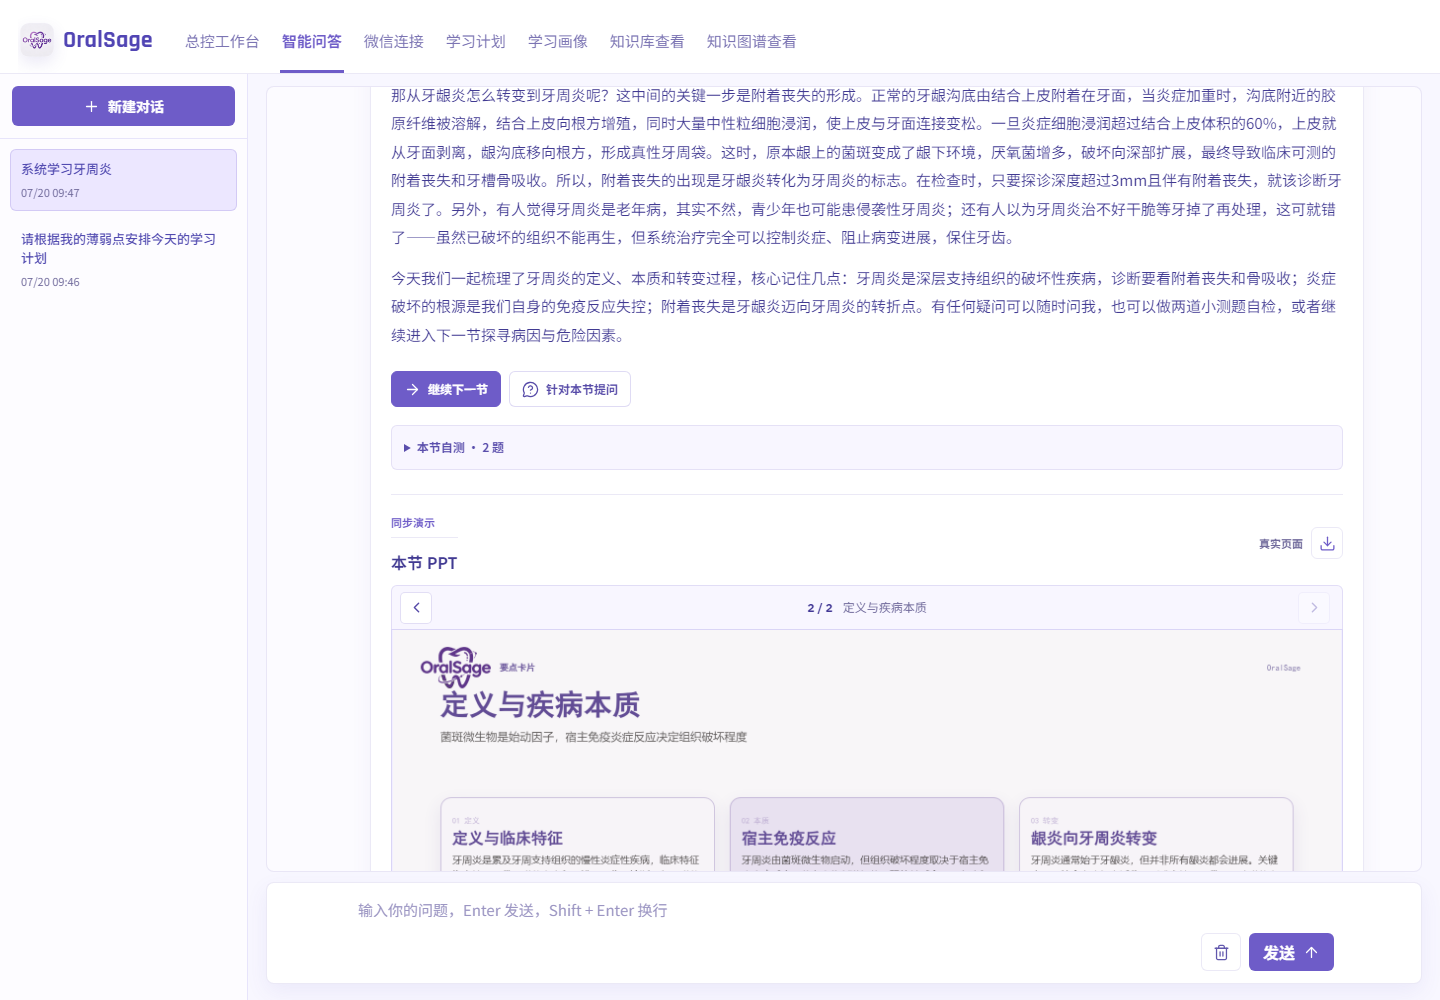
\includegraphics[width=0.92\linewidth]{ui-teaching-result.png}
  \caption{主题学习模式下的连续讲解结果}
  \label{fig:ui-teaching-result}
\end{figure}

在课程学习过程中，学习者可以针对当前讲解内容提出补充问题。系统保留当前学习主题、章节和对话上下文，对问题进行关联回答，避免学习者重新描述背景。当学习者对练习题或自测结果存在疑问时，也可以继续追问题目考点、选项依据和相关知识点，从而形成“讲解—提问—解释—检验”的学习闭环。除课程内答疑外，系统还支持直接输入口腔医学问题进行独立问答，以满足临时知识查询和概念澄清需求。

\begin{figure}[H]
  \centering
  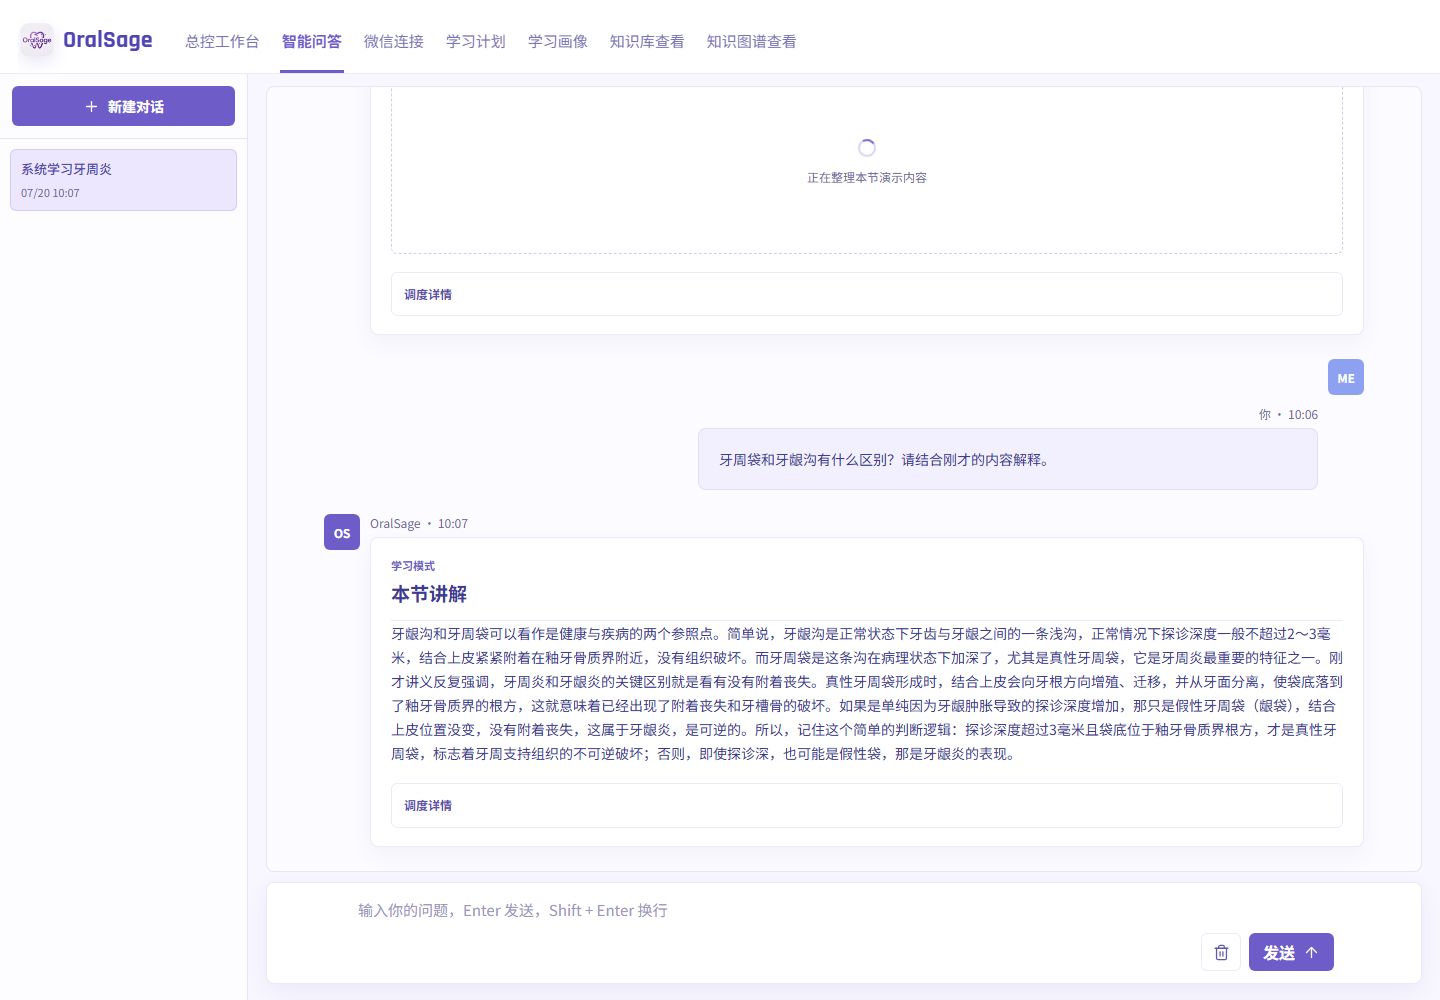
\includegraphics[width=0.92\linewidth]{ui-qa-result.png}
  \caption{课程上下文中的即时答疑结果}
  \label{fig:ui-qa-result}
\end{figure}

问诊模拟页面采用左侧历史记录、中央透明数字人和右侧连续对话区域。学生发送文字或完成语音转写后，医生消息立即进入会话，患者 Agent 的回答由数字人同步播报。正确诊断触发判官接管，后续问题和评分继续出现在同一对话中，页面无需切换到独立考核区。数字人下方只保留当前阶段提示，输入区会随文本内容自动调整高度，减少临床交流中的操作干扰。图~\ref{fig:clinical-speaking-ui}展示了诊断确认后由判官 Agent 接续考核的实际页面，历史问诊、作答输入和当前阶段均保留在同一训练语境中。

\begin{figure}[H]
  \centering
  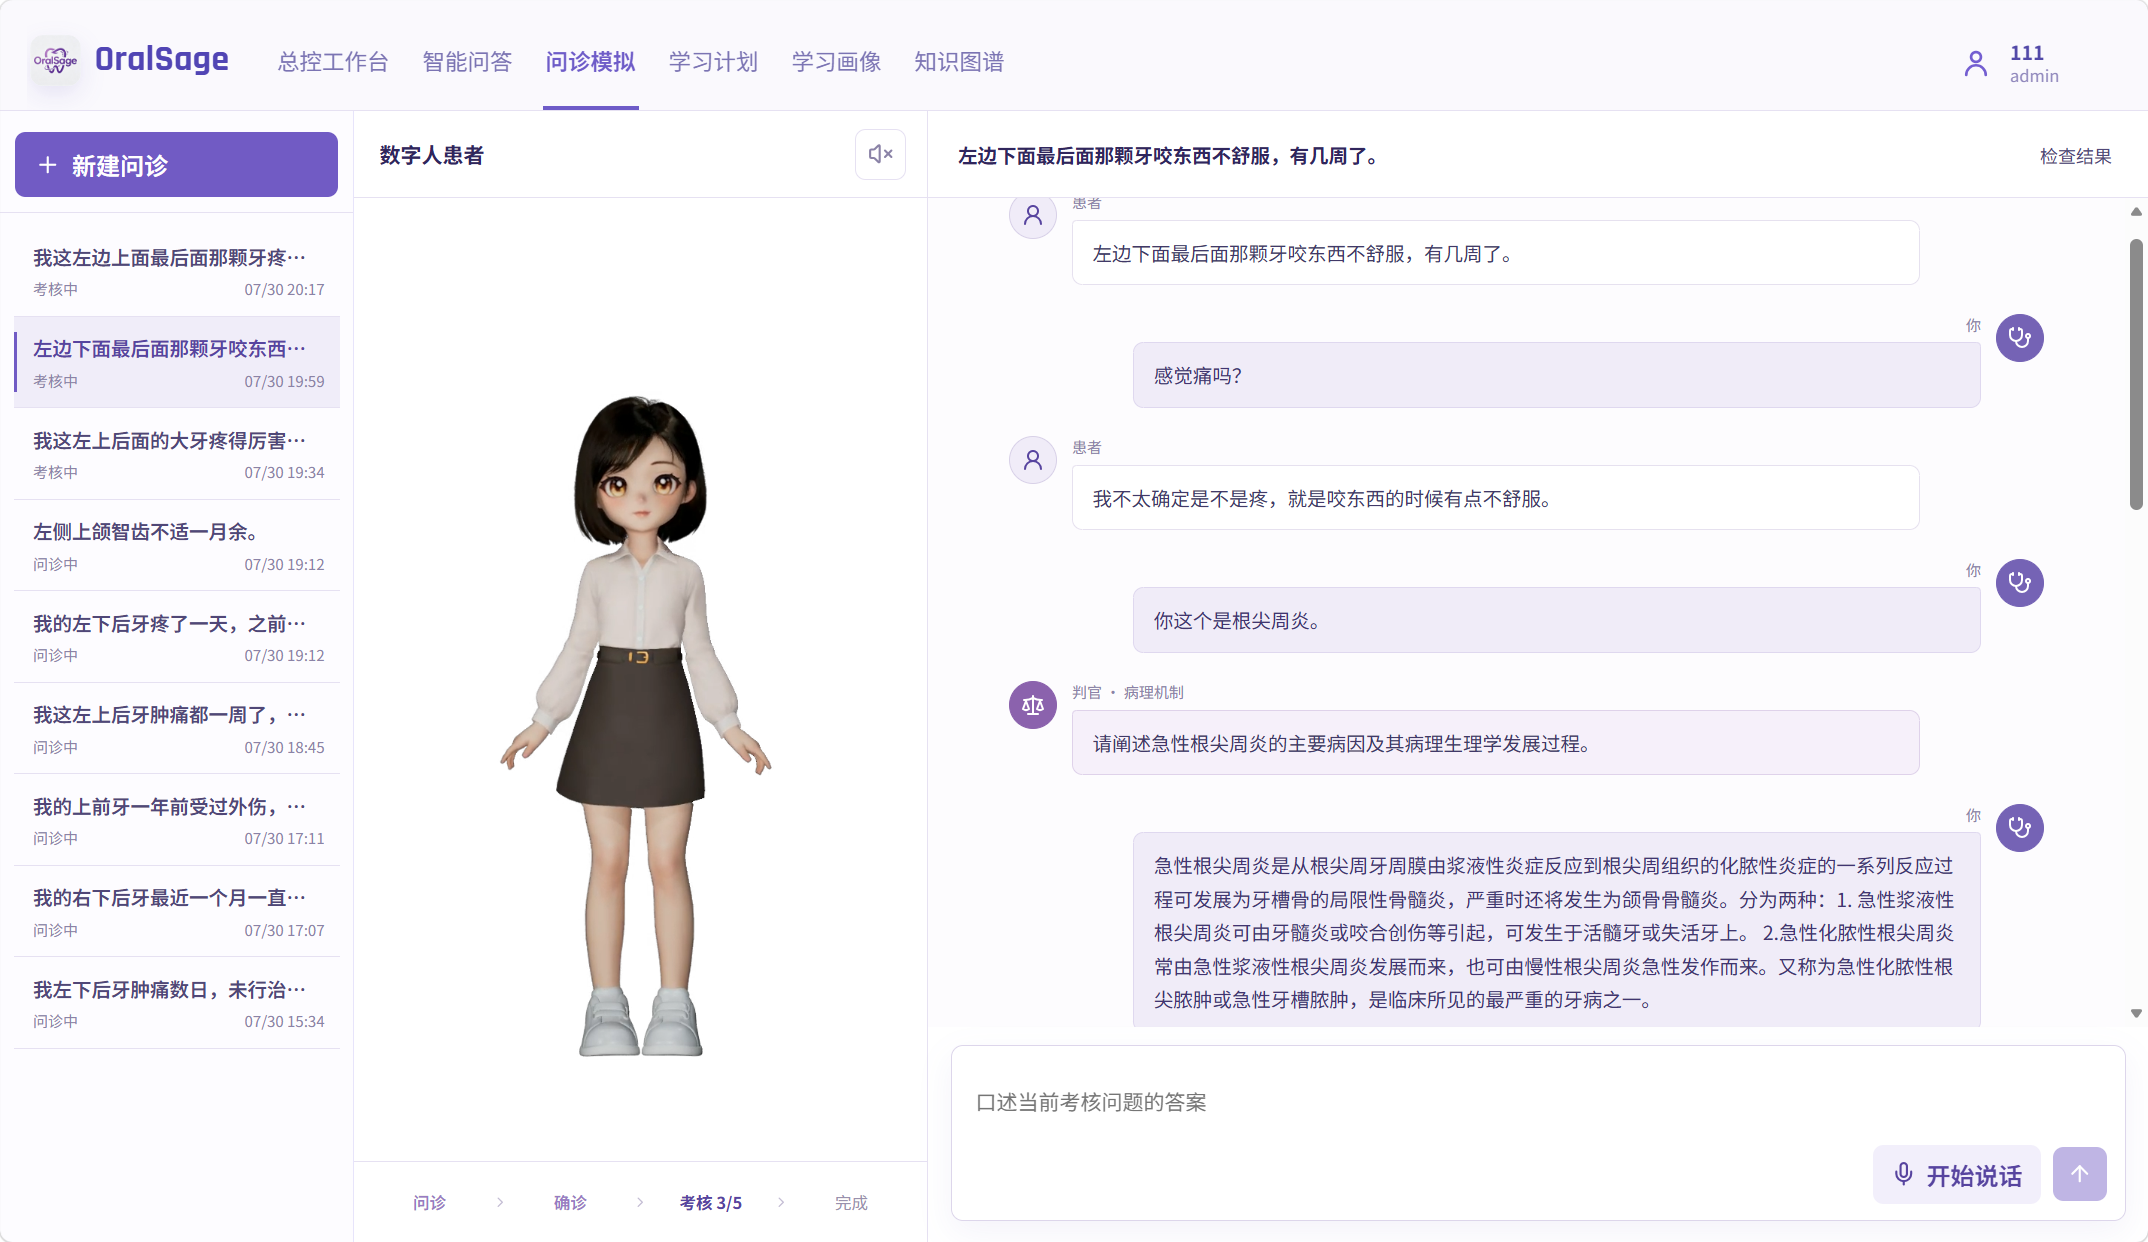
\includegraphics[width=0.92\linewidth]{ui-clinical-speaking.png}
  \caption{数字问诊页面中的患者交互与判官考核}
  \label{fig:clinical-speaking-ui}
\end{figure}

当学习者提出计划需求时，系统能够结合学习画像中记录的薄弱点和用户可用的学习时间组织学习任务。示例中，系统围绕“牙周袋概念混淆”生成学习计划，将章节复习与基础练习拆分为具体任务，并提供进入学习计划页面的操作入口。该设计既保留了通过自然语言提出目标的便捷性，也将生成结果进一步转换为可查看、可执行的任务清单。

\begin{figure}[H]
  \centering
  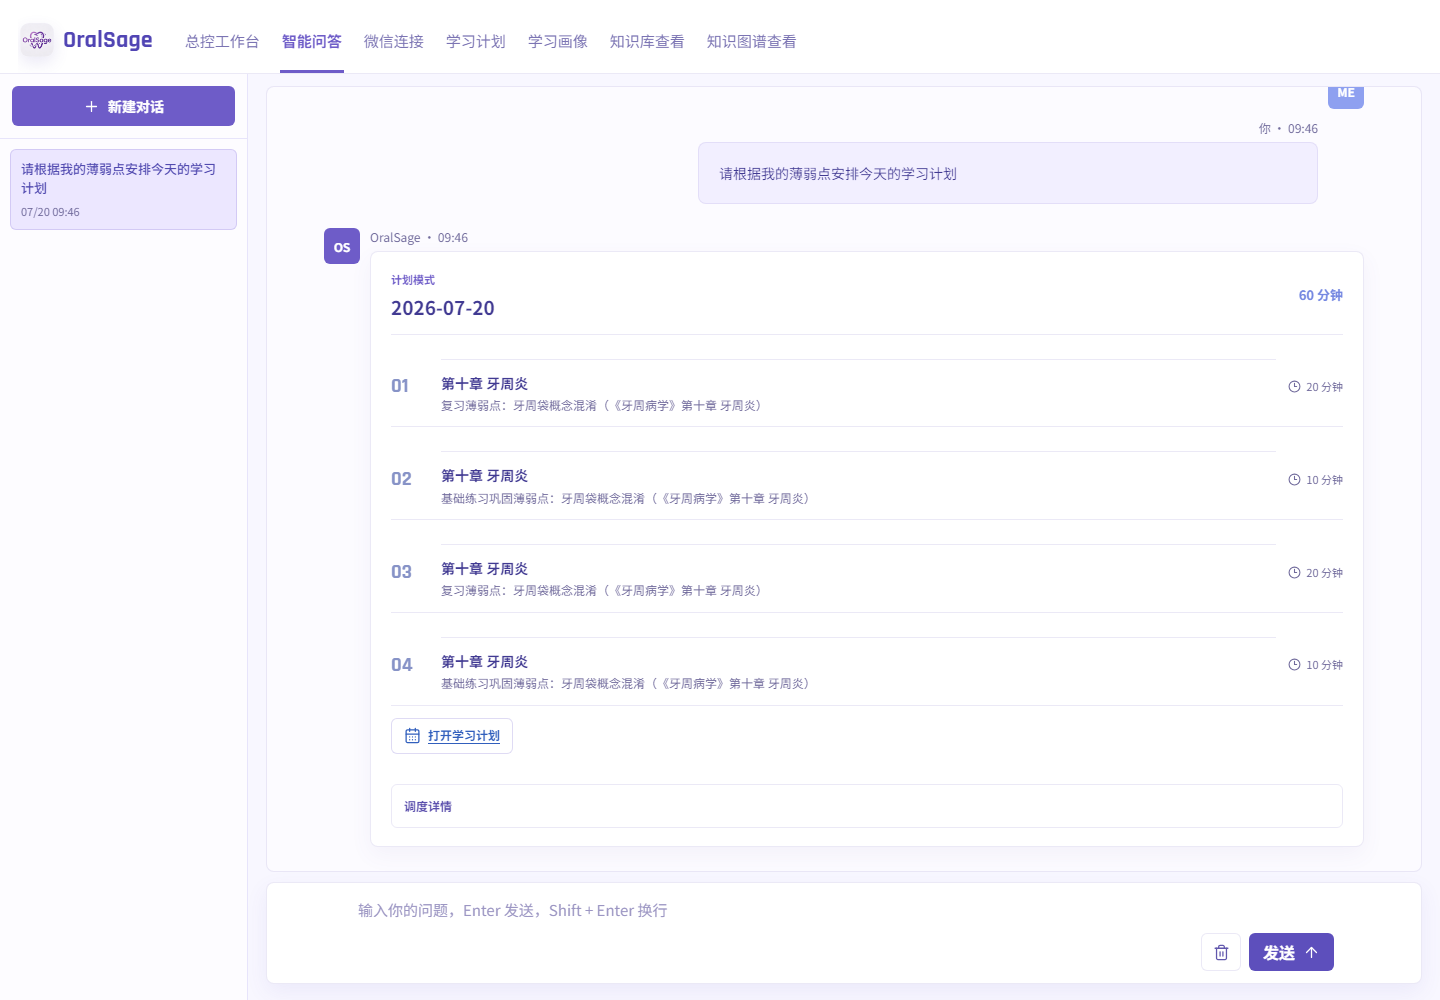
\includegraphics[width=0.92\linewidth]{ui-study-plan-chat.png}
  \caption{通过对话生成学习计划}
  \label{fig:ui-study-plan-chat}
\end{figure}

学习计划并非一次生成后固定不变。学习者可以在计划生成后继续提出时间安排、任务难度或重点内容方面的反馈，系统根据新的约束条件重新组织任务，并将调整结果同步至学习计划页面。由此，计划生成由单向推荐转变为学习者与系统共同调整的过程，使计划内容能够更贴合学习者当前的实际状态。

\begin{figure}[H]
  \centering
  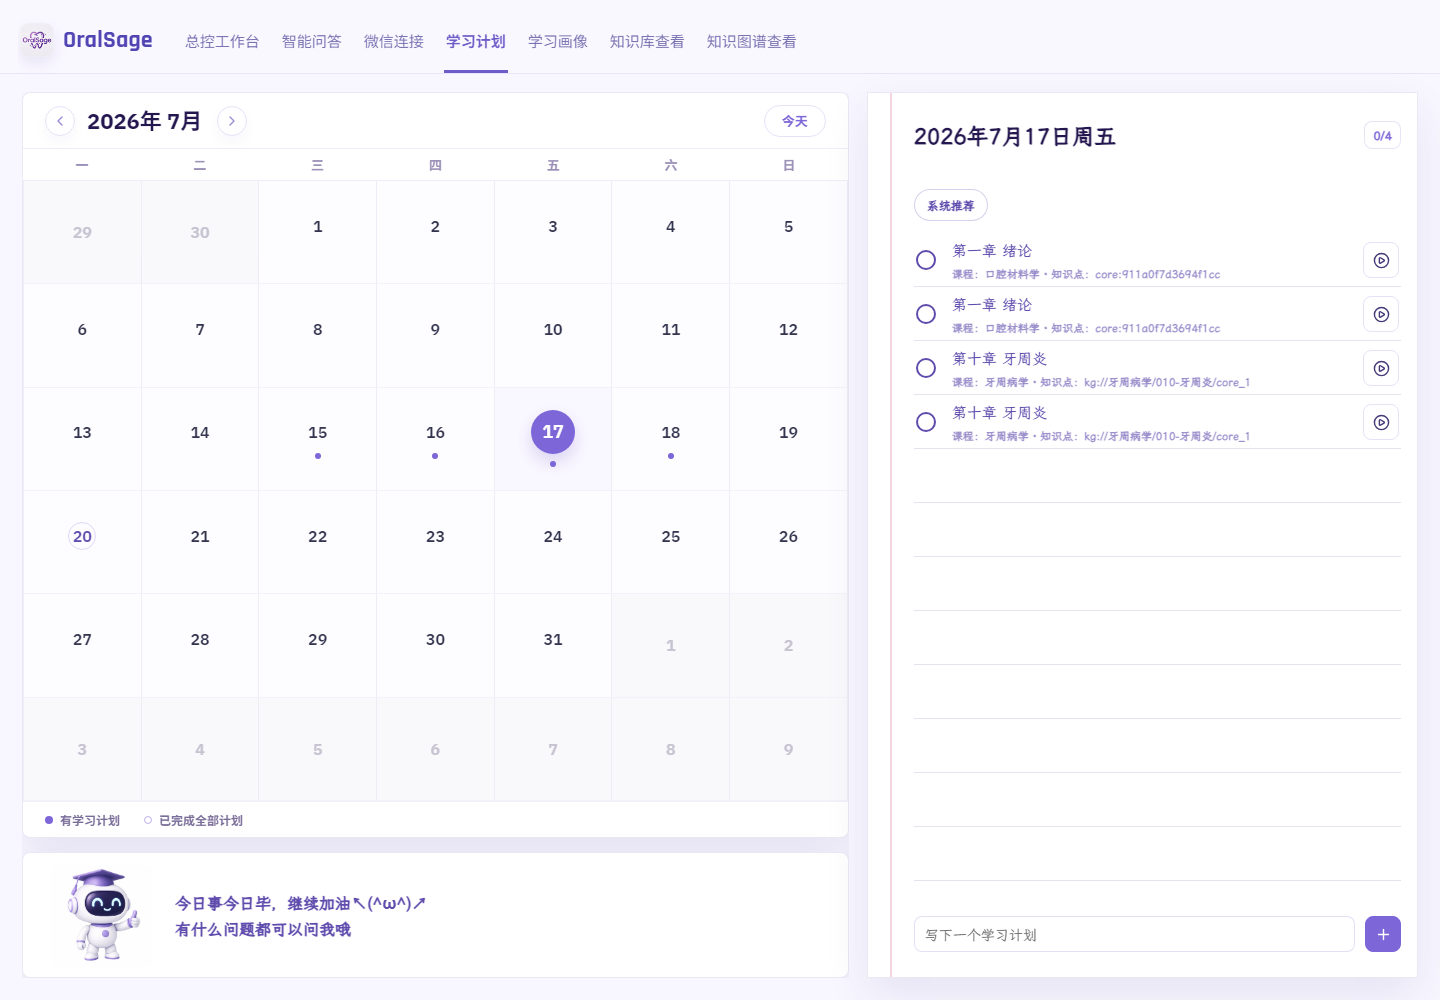
\includegraphics[width=0.92\linewidth]{ui-learning-plan.png}
  \caption{学习计划页面及任务调整入口}
  \label{fig:ui-plan-feedback}
\end{figure}

在文献检索场景中，学习者可以输入检索主题，并设置时间范围和返回数量。页面通过 \texttt{/api/literature/search} 调用文献检索服务并接收 JSON 结果。智能问答中的文献请求由 Router Job 创建任务并通过 SSE 返回进度事件，总控调度器经 MCP Client 调用术语解析、PubMed 和 Scopus 工具。两类请求均使用同一套术语解析、数据源适配与结果整理逻辑，检索编排与工具协议细节见第~\ref{sec:mcp-knowledge-tools}节。检索结果采用列表与详情相结合的双栏布局：左侧集中呈现文献题名、来源、作者和相关度等信息，右侧展示当前选中文献的基本信息及摘要，帮助学习者快速浏览检索结果并查阅与课程主题相关的前沿资料。

\begin{figure}[H]
  \centering
  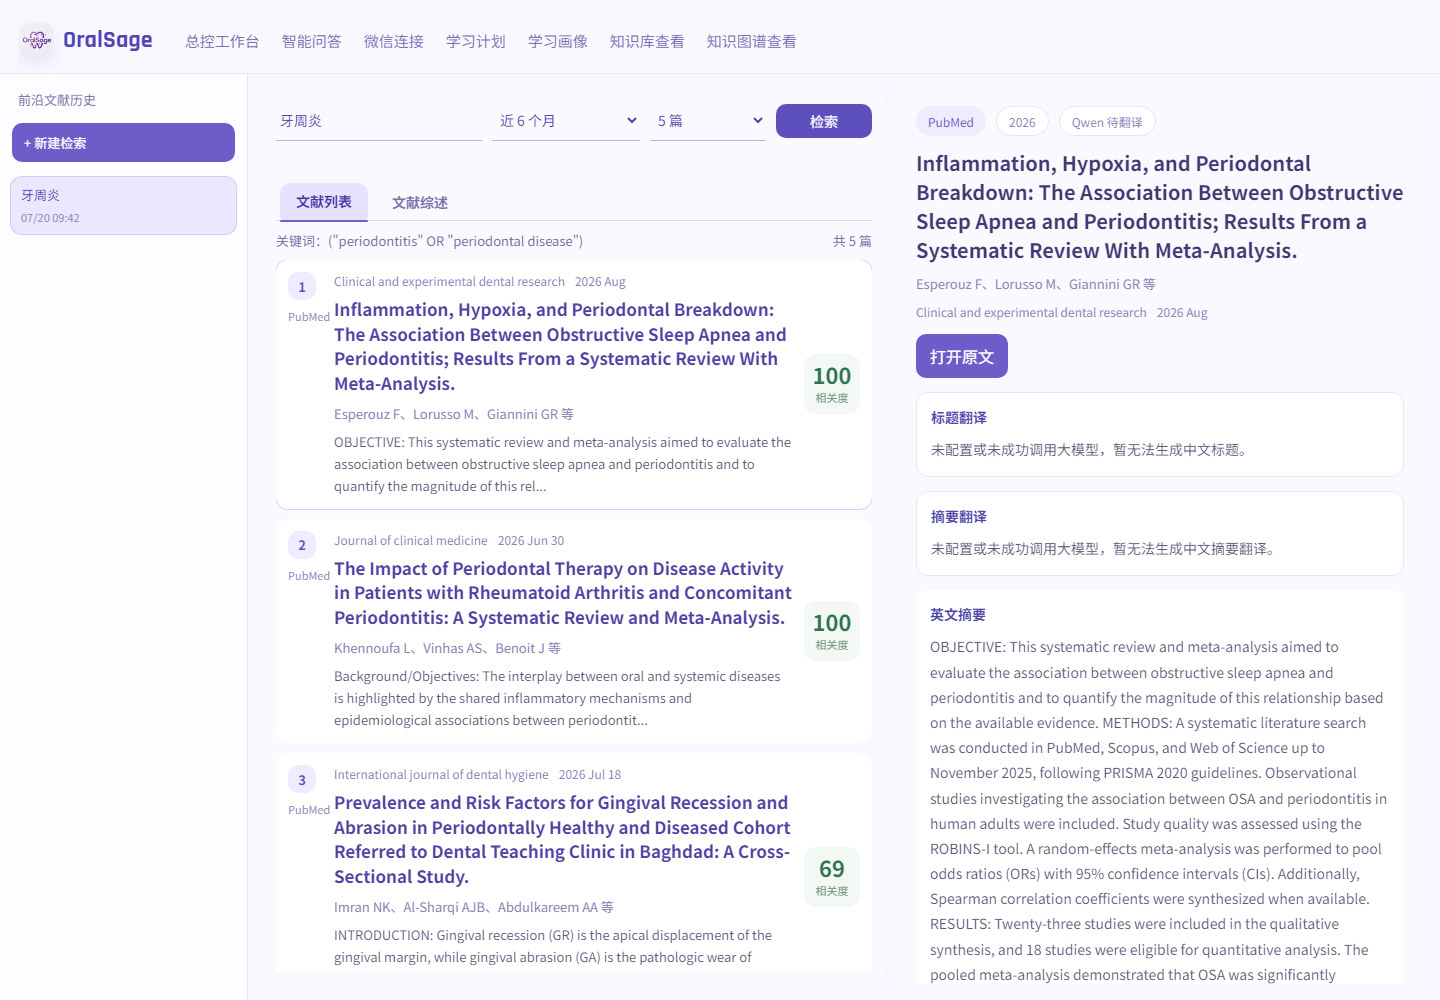
\includegraphics[width=0.92\linewidth]{ui-literature-result.png}
  \caption{前沿文献检索结果}
  \label{fig:ui-literature-result}
\end{figure}

除即时交互外，系统还通过学习画像和学习计划页面呈现持续积累的学习状态。学习画像页汇总近期学习趋势、能力维度、知识薄弱点、学习偏好、目标导向、学习节奏和学习事件，既帮助学习者了解当前学习情况，也为后续课程组织和计划生成提供个性化依据。

\begin{figure}[H]
  \centering
  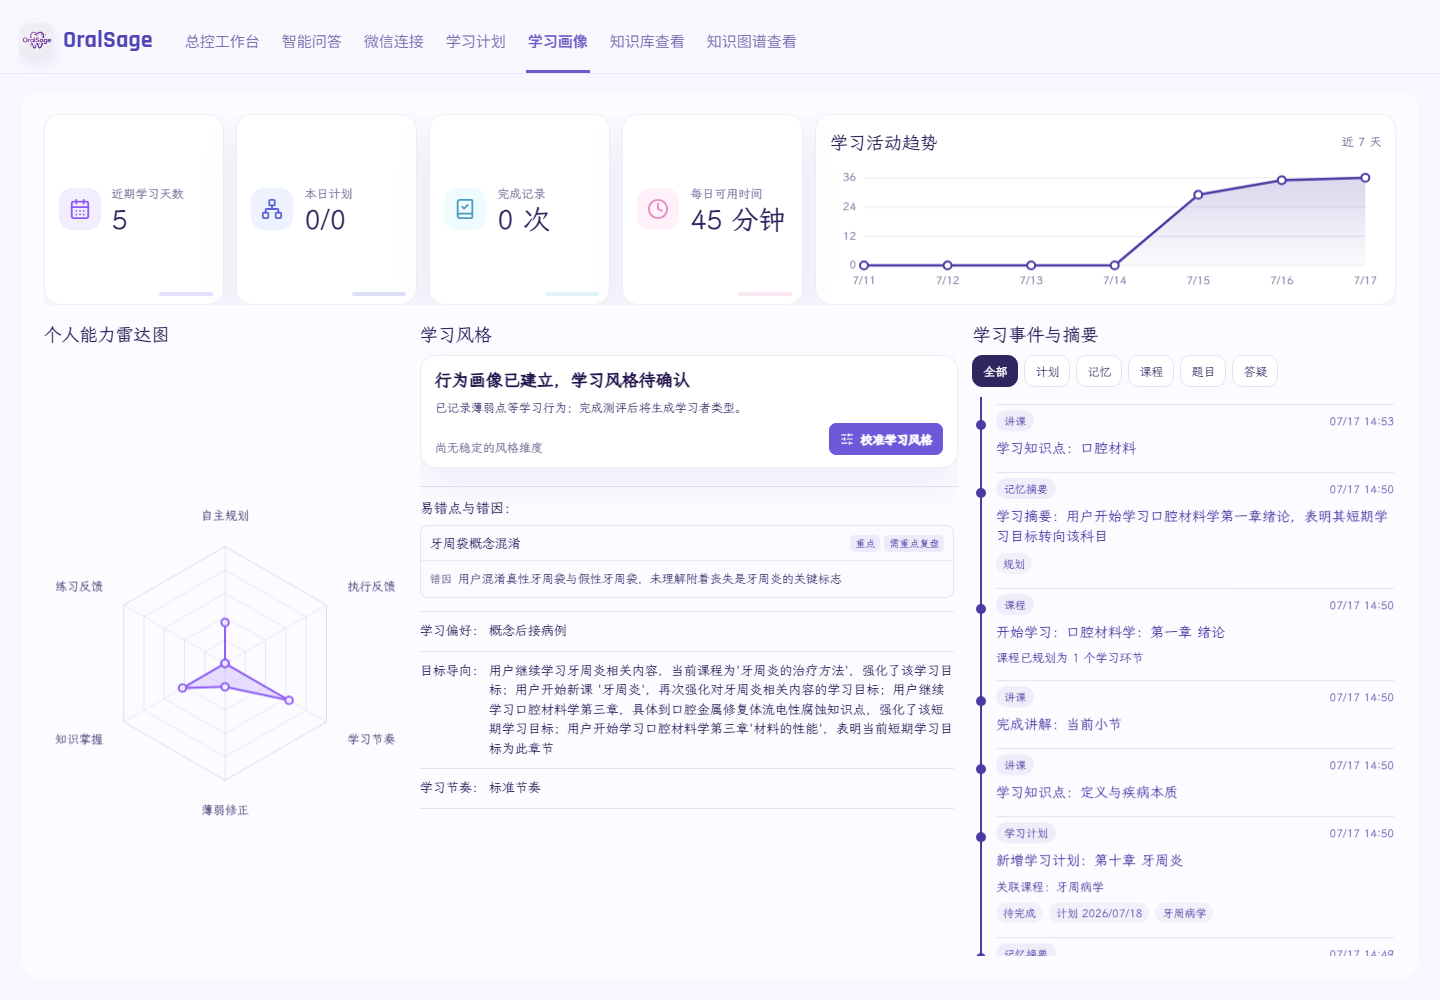
\includegraphics[width=0.92\linewidth]{ui-learning-profile.png}
  \caption{学习画像与学习状态汇总}
  \label{fig:ui-learning-profile}
\end{figure}

学习计划页采用月历与当日任务列表相结合的布局，将系统推荐的学习内容按日期组织，并展示任务所属章节、学习形式和完成状态。学习者可以从具体任务继续进入相应课程。学习画像与学习计划共同将一次性的问答和练习行为沉淀为可持续更新的学习状态与执行安排。

\begin{figure}[H]
  \centering
  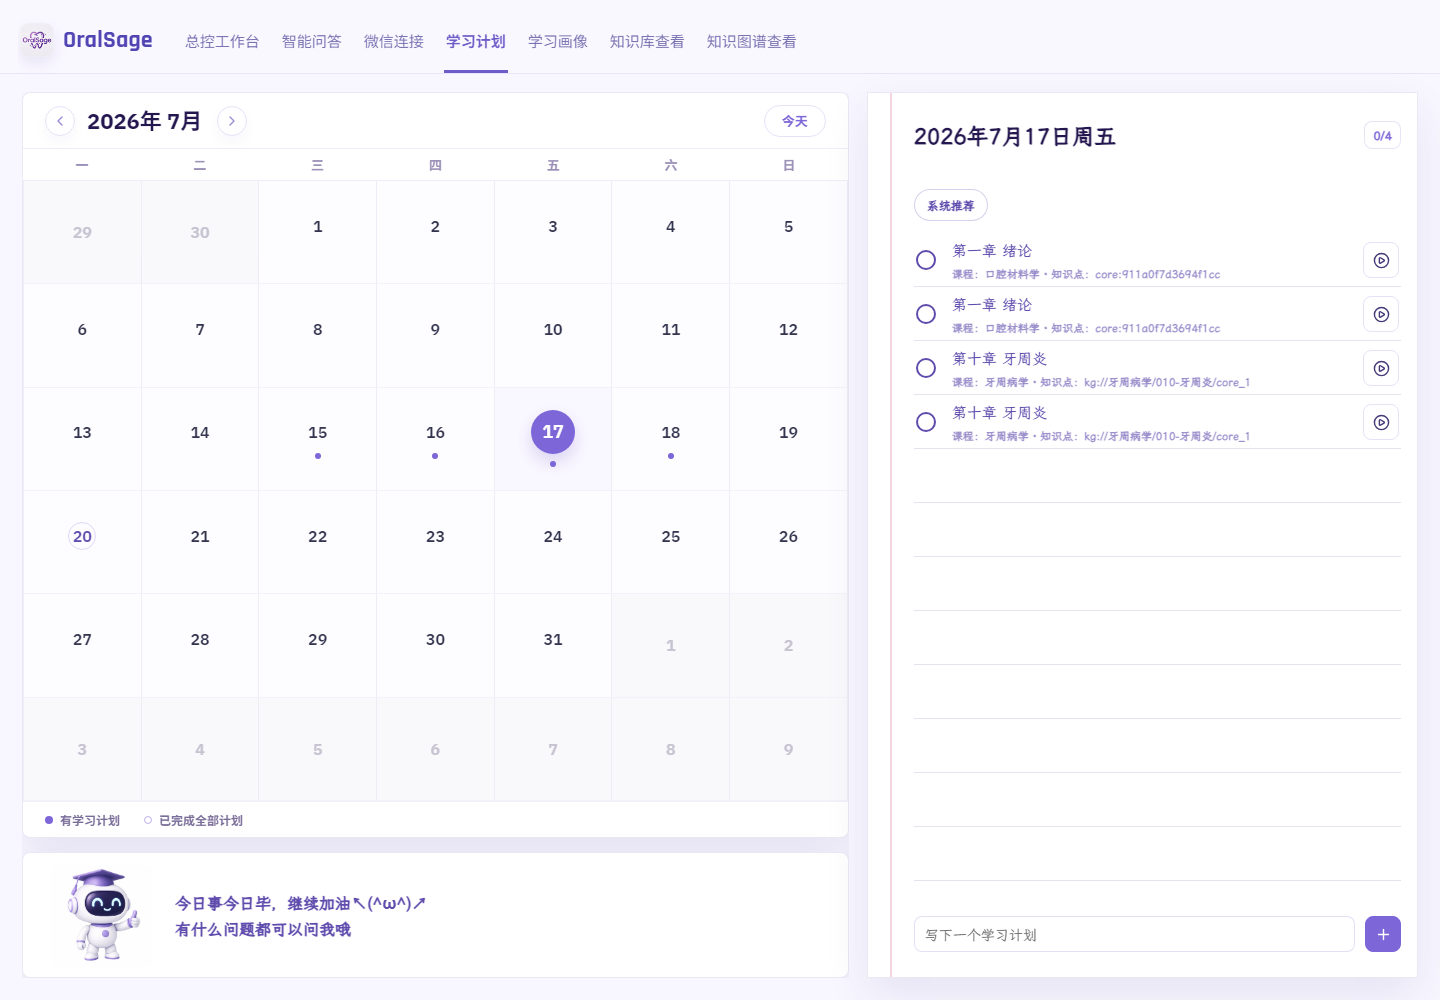
\includegraphics[width=0.92\linewidth]{ui-learning-plan.png}
  \caption{月历式学习计划与任务列表}
  \label{fig:ui-learning-plan}
\end{figure}


\section{数据存储与文件组织}

OralSage 采用“SQLite 持久化学习状态、文件系统保存知识资源和生成资源”的混合存储方式。后端服务负责业务接口、多智能体编排和数据访问，前端目录保存静态页面、样式表和交互脚本，数据目录保存知识库、索引、学习状态和生成文件，模型目录保存本地推理所需的嵌入模型及相关权重，脚本目录用于数据处理、知识库构建和索引生成，测试目录保存接口和核心流程测试，文档目录保存项目说明与辅助材料。

主要目录职责如下：

\begin{itemize}
  \item \texttt{backend/}：包含 FastAPI 接口、请求模型、学习编排器、知识检索、答疑、测评、学习画像和学习计划等后端模块；
  \item \texttt{frontend/}：包含首页、智能问答、问诊模拟、学习画像、学习计划、知识库和知识图谱等页面，以及对应的 JavaScript 交互逻辑和 CSS 样式。
  \item \texttt{data/}：保存知识库文件、检索索引、学习数据库、学习会话资源和微信桥接数据；
  \item \texttt{models/}：保存本地嵌入模型和其他推理模型资源；
  \item \texttt{scripts/}：用于知识库构建、文本切分、索引生成、数据校验和实验性流程运行；
  \item \texttt{tests/}：保存后端接口、学习流程、资源生成和数据处理相关测试；
  \item \texttt{docs/}：保存项目说明、数据处理记录和辅助文档。
\end{itemize}

学习状态和学习画像统一保存在 \texttt{data/learning/learning.sqlite3} 中。数据库以用户和学习会话为主线组织数据，主要包括用户表、用户画像表、学习会话表、课程大纲表、生成资源表、学习事件表、掌握度记录表、答题记录表、学习记忆表、学习摘要表和学习计划任务表。用户画像通过 \texttt{user\_id} 与用户和学习事件关联，学习会话通过 \texttt{session\_id} 关联课程主题、当前大纲节点、讲解过程、答疑记录、练习结果和生成资源，知识掌握度则通过 \texttt{kg\_node\_id} 与知识图谱节点关联。

数字问诊会话保存在 \texttt{data/learning/clinical\_speaking.sqlite3} 中，数据库记录患者对话、状态机阶段、诊断候选、判官题目、分项评分和已处理请求编号。经过确认的诊断与评分结果通过专用事件编号写入 \texttt{learning.sqlite3}，临床训练服务可以独立恢复会话，学习画像也能持续汇总课程与问诊两类学习行为。

综合考试以 \texttt{data/learning/comprehensive\_exams/\{exam\_id\}.json} 保存试卷。文件包含出题时选定的单选题、简答题、题库解析证据、参考答案、评分要点和提交后的评卷结果。考试页面获取试卷时隐藏标准答案、解析和评分要点。提交后服务端读取同一份试卷数据完成答案比对和讯飞星火评阅，再将完整结果返回给页面。

对于课程生成过程中产生的文件，系统以学习会话编号作为资源目录的组织单位，基本路径为：

\begin{lstlisting}
data/learning/sessions/{session_id}/
\end{lstlisting}

该目录用于保存当前课程相关的讲义、课程大纲、思维导图、演示文稿数据、题目、阅读清单、讲稿缓存、音频文件以及 PPT 生成状态等资源。数据库中的生成资源记录保存资源类型、文件路径和来源信息，文件系统保存实际内容，二者通过 \texttt{session\_id} 和资源路径保持对应关系。这样既便于按照学习会话管理生成结果，也支持在前端页面中按需加载讲义、题目、音频和演示资源。

知识库数据与学习状态相互独立。知识库和索引主要以 JSONL、JSON、向量文件和检索索引的形式保存在数据目录中，检索结果通过知识片段标识、知识图谱节点标识和来源信息回写到答疑、课程和学习记忆过程。由此，系统形成了“用户—学习会话—课程节点—知识节点—学习事件—生成资源”的关联链路。

\section{部署与运行方式}

\subsection{本地后端启动}

项目默认在同一 FastAPI 服务中托管后端接口与前端页面。首次运行时进入项目根目录，安装依赖并创建环境配置文件：

\begin{lstlisting}[language=bash,caption={后端本地启动命令},label={lst:backend-start}]
python -m pip install -r backend/requirements.txt
cp .env.example .env
python -m uvicorn backend.main:app --host 127.0.0.1 --port 8000
\end{lstlisting}

Windows PowerShell 环境中，可将第二行替换为：

\begin{lstlisting}[language=bash]
if (-not (Test-Path .env)) { Copy-Item .env.example .env }
\end{lstlisting}

服务启动后，访问 \softid{http://127.0.0.1:8000/} 进入首页，访问 \softid{http://127.0.0.1:8000/docs} 查看接口文档，访问 \softid{http://127.0.0.1:8000/api/system/health} 进行健康检查。开发调试时可增加 \softid{--reload} 参数，使后端代码修改后自动重载。


\subsection{视觉模型服务启动}

若使用本地合并后的 OralPath-VL 模型，可先启动一个兼容 OpenAI 协议的视觉模型服务，再让后端通过 \softid{VISION\_LLM\_*} 访问。以本地 FastAPI 包装服务为例：

\begin{lstlisting}[language=bash,caption={本地视觉模型服务启动示例},label={lst:vision-model-start}]
python openai_vision_server.py
\end{lstlisting}

模型服务默认监听 \softid{8001} 端口，提供 \softid{/v1/models} 和 \softid{/v1/chat/completions}。启动后可使用以下命令检查模型服务：

\begin{lstlisting}[language=bash]
curl http://127.0.0.1:8001/v1/models \
  -H "Authorization: Bearer 12345678"
\end{lstlisting}

对应的后端配置如下：

\begin{lstlisting}[language=bash]
VISION_LLM_API_KEY=12345678
VISION_LLM_BASE_URL=http://127.0.0.1:8001/v1
VISION_LLM_MODEL=oralpath-vl
\end{lstlisting}

完成配置后重启 OralSage 后端，即可在影像识别页面上传口腔影像，完成结构化识别与定位框展示。若部署环境支持 vLLM，也可以将合并模型通过 vLLM 或其他推理框架暴露为同样的 \softid{/v1/chat/completions} 接口，后端配置无需变化。

\subsection{知识库检索依赖}

知识库检索依赖 KAG 制品、BGE-M3 本地模型、FAISS 索引和若干 Python 包。演示环境需要确认 \softid{data/kb/kag\_bge\_m3/} 下存在 \softid{manifest.json}、\softid{chunks.jsonl}、\softid{retrieval\_corpus.jsonl}、\softid{kg\_nodes.jsonl} 以及 \softid{indexes/} 子目录，并确认 \softid{models/embeddings/bge-m3} 可用。推荐安装：

\begin{lstlisting}[language=bash]
python -m pip install jieba faiss-cpu onnxruntime transformers
\end{lstlisting}

部署后可通过以下命令检查知识检索接口：

\begin{lstlisting}[language=bash]
curl -X POST http://127.0.0.1:8000/api/knowledge/search \
  -H "Content-Type: application/json" \
  -d '{"query":"牙周炎","top_k":3}'
\end{lstlisting}

若返回 \softid{ok=true} 且 \softid{results} 中包含检索片段，说明知识库页面和智能体检索链路已正常工作。

\subsection{微信 ClawBridge 启动}

微信接入服务位于 \softid{clawbridge/}，采用 Node.js 实现，主要负责二维码绑定、微信会话状态维护、消息转发和计划推送。它不承担学习业务逻辑，而是将微信侧消息转交 Python 后端处理。启动方式如下：

\begin{lstlisting}[language=bash,caption={ClawBridge 启动命令},label={lst:clawbridge-start}]
cd clawbridge
npm install
npm run start
\end{lstlisting}

ClawBridge 默认监听 \softid{8787} 端口。Python 后端通过 \softid{CLAWBRIDGE\_BASE\_URL} 和共享内部密钥访问该服务，从而完成微信账户绑定状态查询、学习计划推送和消息回传。

\section{第三方组件与工具说明}

项目仅列出运行时直接使用的主要组件，传递依赖不单独展开。版本以项目依赖声明为准，具体许可证以组件随附的许可证文件和官方发布信息为准。

\begin{table}[H]
\centering
\small
\begin{tabularx}{\linewidth}{p{3.2cm}p{2.5cm}X p{2.5cm}}
\toprule
组件或工具 & 版本/来源 & 在项目中的使用位置 & 许可证或协议 \\
\midrule
FastAPI & 0.136.1 & 提供后端 HTTP 接口和静态页面服务 & MIT \\
Uvicorn & 0.46.0 & 运行 FastAPI 应用的 ASGI 服务 & BSD-3-Clause \\
Pydantic & 2.13.3 & 定义请求、响应和配置数据模型 & MIT \\
LangGraph & 1.1.9 & 支持多智能体工作流和任务编排 & MIT \\
PyYAML & 6.0.2 & 读取检索和系统配置文件 & MIT \\
pypdf & 6.4.1 & 解析和处理 PDF 文档 & BSD-3-Clause \\
openpyxl & 3.1.5 & 处理 Excel 格式的结构化数据 & MIT \\
NumPy & 2.4.6 & 支持向量计算、数据处理和索引构建 & BSD-3-Clause \\
SQLite & 系统组件 & 保存用户、学习会话、画像、答题和计划数据 & Public Domain \\
BGE-M3 & 本地模型文件 & 生成知识片段的向量表示并支持语义检索 & 依模型发布许可 \\
Lucide Icons & 前端 CDN 组件 & 提供前端页面中的图标资源 & ISC \\
ClawBot Bridge & package.json 声明版本 & 连接微信学习场景并推送学习计划 & 依 npm 包及桥接组件许可 \\
\bottomrule
\end{tabularx}
\caption{项目主要第三方组件与工具}
\end{table}

其中，BGE-M3 模型以本地文件形式加载，运行时不要求将知识库内容上传至外部检索服务。ClawBot Bridge 作为独立的 Node.js 辅助服务，用于连接微信学习场景和学习计划推送，不参与核心课程生成逻辑。项目开发过程中使用 AI Coding 工具辅助代码检索、调试和文档整理，该工具属于开发辅助工具，不是系统运行时依赖，也不参与用户请求处理。

\chapter{测试与评估}
\label{sec:testing}

\section{测试目标与测试范围}

本章围绕 OralSage 的功能完整性、智能体协同、知识检索、资源生成、学习测评、数字问诊、证据一致性和核心响应时间开展测试。测试覆盖学习者从进入系统、建立学习画像、输入学习目标、生成学习计划，到获得课程讲解、进行即时答疑、完成练习并更新学习状态的主要过程，也覆盖数字人患者问诊、自然语言诊断理解、判官接管和临床表达评分。

测试采用自动化测试与真实功能链路测试相结合的方式。自动化测试用于验证后端服务、前端交互逻辑、状态转换和异常处理；真实功能测试使用项目本地知识库、知识图谱、稀疏索引、稠密向量索引和模型服务，验证课程规划、讲义生成、Tutor 讲解和 QA 答疑等模块的实际运行结果。

\begin{table}[H]
  \centering
  \caption{测试环境与测试范围}
  \label{tab:test-environment}
  \begin{tabularx}{\linewidth}{p{0.25\linewidth}X}
    \toprule
    测试项目 & 配置与范围 \\
    \midrule
    运行环境 & Windows 本地运行环境 \\
    后端服务 & OralSage 本地服务，测试地址为 \texttt{127.0.0.1:8000} \\
    自动化测试 & Python 后端测试和 Node.js 前端逻辑测试 \\
    知识检索 & 本地 KAG 检索服务、稀疏倒排索引和 BGE-M3 稠密向量索引 \\
    检索语料 & 34,805 条统一文本片段 \\
    测试主题 & 以“牙周炎”等口腔医学主题为主要测试对象 \\
    测试模块 & 学习画像、学习计划、课程规划、资源生成、Tutor 讲解、QA 答疑、数字问诊、学习测评和状态更新 \\
    \bottomrule
  \end{tabularx}
\end{table}

\section{自动化测试结果}

Python 后端测试共执行 961 项，覆盖学习路由、课程规划、知识检索、学习计划、画像状态、资源生成、即时答疑、测评、缓存和状态持久化等模块，全部完成。

数字问诊功能新增 49 项专项测试，涉及临床训练服务、学习画像事件和实时数字人配置，全部通过。该组测试独立验证患者 Agent、判官 Agent、病例仓库、讯飞语音听写配置、数字人鉴权与画像反馈，便于对新增链路进行集中复核。

前端测试覆盖学习计划草稿加载、计划项目采用、依赖关系处理、主对话状态、学习会话参数和计划入口。其中，学习计划草稿测试完成 60 项，主对话计划草稿测试完成 76 项，主对话测试完成 51 项，学习计划逻辑测试完成全部测试项。

\begin{table}[H]
  \centering
  \caption{自动化测试结果}
  \label{tab:automated-test}
  \begin{tabularx}{\linewidth}{p{0.30\linewidth}p{0.28\linewidth}X}
    \toprule
    测试项目 & 实际结果 & 覆盖内容 \\
    \midrule
    Python 后端测试 & 961 项完成且无失败项 & 路由、规划、检索、资源生成、答疑、测评、画像、缓存与状态管理 \\
    数字问诊专项测试 & 49 项完成且无失败项 & 病例选题、患者交互、诊断识别、判官评分、语音、数字人、状态与画像事件 \\
    学习计划草稿测试 & 60 项完成且无失败项 & 草稿加载、课程范围、推荐卡片、采用请求和异常处理 \\
    主对话计划草稿测试 & 76 项完成且无失败项 & 计划草稿保存、会话切换、计划采用、依赖关系和页面参数 \\
    主对话测试 & 51 项完成且无失败项 & 学习请求、文献请求、答疑、会话状态和学习计划入口 \\
    学习计划逻辑测试 & 测试项全部完成 & 计划生成、计划项目数据和前端状态转换 \\
    \bottomrule
  \end{tabularx}
\end{table}

\section{核心功能测试}

核心功能测试以真实学习流程为对象，验证用户输入是否能够转化为课程规划、学习资源和学习状态。

输入“牙周炎”后，系统生成 5 个课程节点，并为当前课程节点绑定知识节点和资料片段。后续讲义、Tutor 和 QA 均基于该课程节点继续执行。

\begin{table}[H]
  \centering
  \caption{核心功能测试结果}
  \label{tab:function-test}
  \begin{tabularx}{\linewidth}{p{0.27\linewidth}X}
    \toprule
    测试功能 & 实际结果 \\
    \midrule
    学习画像 & 初始画像包含本科高年级、期末考试、病例带入和标准节奏等字段；提问和答题后，薄弱点由空集更新为“机制链条不完整、牙槽骨吸收、牙龈炎与牙周炎区别” \\
    主题学习 & 输入“牙周炎”，生成 5 个课程节点 \\
    学习计划 & 生成计划草稿，保存课程范围、计划项目、日期和依赖关系 \\
    计划反馈修改 & 草稿能够被读取、修改并重新进入计划采用流程 \\
    文献检索 & 输入文献主题后返回对应检索结果 \\
    MCP 工具调用 & 客户端完成初始化、工具发现和结构化调用，知识库检索、术语解析、PubMed 与 Scopus 四项工具均可被识别和调用 \\
    文献调用链路 & 页面接口返回 HTTP JSON，Router Job 可创建任务、查询状态并通过 SSE 重放进度事件 \\
    课程讲解 & Tutor 返回 \texttt{llm\_generated} 内容 \\
    当前章节答疑 & 返回 \texttt{llm\_generated} 内容，未推进课程进度 \\
    课程延伸答疑 & 返回 \texttt{llm\_generated} 内容，并生成 2 条定向检索计划 \\
    学习测评 & 完成题目生成、答案提交、批改、解析和掌握度更新 \\
    学习状态 & 完成课程进度、学习事件、答案记录和掌握度记录保存 \\
    \bottomrule
  \end{tabularx}
\end{table}

\section{智能体协同链路测试}

主题学习流程中的智能体调用顺序为：Planner 根据主题、学习者画像和检索证据生成课程结构；Resource Factory 根据当前课程节点生成讲义；Tutor 根据讲义和证据生成讲解；QA 根据问题范围选择当前证据或发起定向检索；Assessment 负责练习与阶段测评；Memory/User Model 保存学习事件、掌握度和薄弱知识点。

\begin{table}[H]
  \centering
  \caption{智能体协同链路测试结果}
  \label{tab:agent-chain-test}
  \begin{tabularx}{\linewidth}{p{0.25\linewidth}X}
    \toprule
    测试环节 & 实际结果 \\
    \midrule
    Planner & 输入“牙周炎”，生成 5 个课程节点，并为首节点绑定 1 个知识节点和 2 条资料片段 \\
    Resource Factory & 生成首节讲义，返回 177 字概述和 4 个主要知识点 \\
    Tutor & 基于首节讲义生成 \texttt{llm\_generated} 讲解内容 \\
    QA 当前章节模式 & 问题范围为 \texttt{in\_current\_section}，使用 2 条证据直接回答 \\
    QA 延伸检索模式 & 问题范围为 \texttt{course\_related\_but\_not\_current}，生成 2 条检索计划并使用 4 条证据回答 \\
    Assessment & 完成错误答案识别、解析、错因信息和掌握度更新 \\
    Memory/User Model & 答题后更新薄弱点、错误模式和掌握度记录 \\
    Orchestrator & 完成 Planner、Resource Factory、Tutor、QA、Assessment 和 Memory/User Model 的连续调度 \\
    \bottomrule
  \end{tabularx}
\end{table}

两类答疑的 \texttt{advance\_progress} 均为 \texttt{False}，说明用户在课程中插入问题不会导致课程进度被错误推进。

\section{数字问诊专项测试}

专项测试围绕第~\ref{sec:digital-consultation}节的完整流程展开。病例仓库测试检查训练字段完整性、复诊记录排除、直接身份信息清理，以及先选疾病类别再抽取病例的随机选题顺序。患者 Agent 测试使用不同语气的自然语言诊断和追问，检查意图理解、事实编号引用、未知信息处理与疾病名称隐藏，确认患者回复不会直接暴露目标诊断。

患者与判官交接测试覆盖明确诊断识别、诊断复核、用户确认和首道考核题生成。判官测试检查五个考核领域的检索覆盖、题目证据集合、分值范围、批评意见结构和画像写入，非法证据编号无法进入有效评分结果。请求编号测试重复提交会话创建、问诊轮次和考核回答，确认问题序号、分数与学习事件只更新一次。

语音与数字人测试检查讯飞听写签名地址不会泄露 APISecret，医学术语整理会保留学生原始诊断语义，语音输入完成后能够进入患者 Agent。浏览器交互测试还覆盖消息即时显示、输入框自动高度和音频末帧提交，数字人公开配置仅包含建立实时互动所需的参数。49 项专项测试全部通过，结果如表~\ref{tab:clinical-speaking-test} 所示。

\begin{table}[H]
  \centering
  \caption{数字问诊专项测试结果}
  \label{tab:clinical-speaking-test}
  \begin{tabularx}{\linewidth}{p{0.28\linewidth}X}
    \toprule
    检查类别 & 已验证行为 \\
    \midrule
    病例与选题 & 完整字段过滤、脱敏输出、疾病类别随机选择和画像目标映射 \\
    患者交互 & 自然语言意图理解、病例事实约束、未知信息表达和诊断隐藏 \\
    诊断交接 & 明确诊断判断、独立复核、用户确认和判官接管 \\
    判官评分 & 五域证据检索、问题结构、评分范围、批评意见和合法证据引用 \\
    状态与重复请求 & 会话恢复、请求编号复用、并发写入顺序和题目进度保护 \\
    语音与数字人 & 听写签名保护、术语整理、音频提交、数字人公开配置和透明画面尺寸 \\
    学习画像 & 问诊事件分类、分项掌握度、薄弱点和时间线筛选 \\
    \bottomrule
  \end{tabularx}
\end{table}

\section{综合考试专项测试}

综合考试专项测试聚焦讯飞响应处理、简答题命题约束、评阅结果处理和结果展示。服务按照十五道单选题与五道简答题组织试卷。画像切片提供薄弱知识点后，候选题目排序会优先考虑相关题目。缺少画像信息时，系统从可用题目中完成试卷抽取。

简答题测试检查讯飞星火返回的题干、题型、参考答案和评分要点。每道简答题关联一条题库解析证据，命题结果需覆盖五条独立证据。评卷测试为每道简答题提交学生答案，并检查讯飞星火返回零至五分的得分、反馈文本和缺失要点。单选题得分由服务端直接比对题库答案，结果中同时保留解析内容。相关用例位于 \texttt{tests/test\_comprehensive\_exam.py}。

\begin{table}[H]
  \centering
  \caption{综合考试专项测试内容}
  \label{tab:comprehensive-exam-test}
  \begin{tabularx}{\linewidth}{p{0.28\linewidth}X}
    \toprule
    检查类别 & 已验证行为 \\
    \midrule
    响应契约 & 解析单项 JSON、常见外层包装和序列化对象，检查题干、题型、参考答案与评分要点 \\
    传输切换 & 首次响应未返回内容时切换调用方式，短暂请求异常后继续获取讯飞响应 \\
    服务端绑定 & 将命题证据标识和评卷题目编号由服务端写入结果，保持题目、证据和得分的对应关系 \\
    题型规范 & 将概念、病例诊断和单选改写等有效题型归一化，检查评分要点数量与内容完整性 \\
    画像输入 & 将画像中的薄弱知识点压缩为受限知识侧重信息，再交由讯飞星火参与简答题命题 \\
    结果展示 & 提交后的公开结果保留单选解析、简答题参考答案和评分要点，供结果页完整呈现 \\
    \bottomrule
  \end{tabularx}
\end{table}

\section{资源生成测试}

资源生成测试覆盖讲义、Tutor 讲解、思维导图、练习题、阶段卷、PPT/slides 和音频。

首节讲义测试中，当前课程节点绑定 1 个知识节点和 2 条资料片段。生成结果包含 1 段 177 字的课程概述和 4 个主要知识点，分别涉及牙周炎的定义与疾病性质、牙周炎与牙龈病的区别、始动因素与全身促进因素，以及临床表现与疾病进展。

\begin{table}[H]
  \centering
  \caption{资源生成测试结果}
  \label{tab:resource-test}
  \begin{tabularx}{\linewidth}{p{0.27\linewidth}X}
    \toprule
    资源类型 & 实际结果 \\
    \midrule
    首节讲义 & 1 个知识节点、2 条资料片段、177 字概述、4 个主要知识点 \\
    Tutor 讲解 & 返回 \texttt{llm\_generated} 内容 \\
    思维导图 & 根据 5 个课程节点生成课程结构 \\
    练习题 & 根据课程内容和知识节点生成题目 \\
    阶段卷 & 完成题目、答案、批改和结果返回 \\
    PPT/slides & 单页资源文件生成成功，资源路径存在；两步流程能够合并为完整 deck \\
    音频 & 讲解音频生成链路返回有效资源状态 \\
    \bottomrule
  \end{tabularx}
\end{table}

\section{学习测评与学习状态测试}

学习测评测试检查题目生成、答案提交、自动批改、答案解析、错因识别、薄弱知识节点更新和补救建议生成。

在学习状态测试中，用户先提交 1 次错误答案，系统生成 1 条答案记录和至少 1 条掌握度记录；随后提交正确答案，答案记录增加到 2 条，掌握度记录保持存在且掌握度分数发生变化。课程节点在答题和答疑过程中保持不变。

\begin{table}[H]
  \centering
  \caption{学习测评与状态更新结果}
  \label{tab:assessment-test}
  \begin{tabularx}{\linewidth}{p{0.35\linewidth}X}
    \toprule
    检查项目 & 实际结果 \\
    \midrule
    题目生成 & 依据当前课程节点生成带选项和正确答案的题目 \\
    错误答案处理 & \texttt{is\_correct=False}，保存用户选项和正确选项 \\
    错误解析 & 返回选项错误分析、正确答案解释和误解概述 \\
    错误后进度 & 当前课程节点保持不变 \\
    错误后画像 & 薄弱点和错误模式发生更新 \\
    掌握度记录 & 错误答案后新增或更新掌握度记录 \\
    正确答案处理 & 答案记录总数增加到 2 条 \\
    掌握度变化 & 正确答案后掌握度分数发生变化 \\
    答案持久化 & 会话摘要中包含 \texttt{answers} 字段 \\
    补救建议 & 根据错误知识节点生成后续学习建议 \\
    \bottomrule
  \end{tabularx}
\end{table}

用户模型测试还验证了画像从初始状态到学习中状态的变化：初始画像为本科高年级、期末考试、偏好病例带入、标准节奏、暂无薄弱点；中途提问后增加“机制链条不完整”和“牙槽骨吸收”两个薄弱点；答错题后进一步增加“牙龈炎与牙周炎区别”；最终画像的偏好调整为“先病例后概念”，节奏调整为“慢一点”。

\section{知识检索与证据一致性测试}

真实 KAG 检索测试成功加载 34,805 条文本片段，同时加载稀疏倒排索引和 BGE-M3 稠密向量索引。以“牙周炎”为检索词时，系统返回 5 条相关结果，并展示前 3 条结果。结果来源包括牙周病学教材、口腔组织病理学教材和临床医学资料。

\begin{table}[H]
  \centering
  \caption{KAG 检索结果}
  \label{tab:kag-retrieval-test}
  \begin{tabularx}{\linewidth}{p{0.34\linewidth}X}
    \toprule
    检查项目 & 实际结果 \\
    \midrule
    文本片段加载 & 34,805 条 \\
    稀疏倒排索引 & 加载成功 \\
    BGE-M3 稠密索引 & 加载成功 \\
    “牙周炎”检索 & 返回 5 条结果 \\
    结果展示 & 展示前 3 条结果 \\
    资料来源 & 教材、医学手册和知识库资料 \\
    \bottomrule
  \end{tabularx}
\end{table}

课程节点的证据绑定和答疑过程均使用当前证据池中的合法标识。当前章节答疑使用 2 条证据；课程延伸答疑在定向检索后使用 4 条证据。非法知识节点或文本片段标识无法进入有效规划结果，模型返回的不同证据字段也能够被统一处理。

\section{响应时间测试}

响应时间测试使用本地后端真实学习接口完成，测试主题为“牙周炎”。

\begin{table}[H]
  \centering
  \caption{核心学习流程响应时间}
  \label{tab:latency-test}
  \begin{tabularx}{\linewidth}{p{0.40\linewidth}p{0.22\linewidth}X}
    \toprule
    测试阶段 & 实测耗时 & 实际结果 \\
    \midrule
    首节课程大纲就绪 & 145.088 秒 & 生成 5 个课程节点 \\
    首节讲义缓存就绪 & 随首节资源流程完成 & 缓存状态为 \texttt{ready} \\
    Tutor 首次内容就绪 & 195.103 秒 & 内容状态为 \texttt{llm\_generated} \\
    完整学习请求完成 & 195.103 秒 & 接口返回成功 \\
    \bottomrule
  \end{tabularx}
\end{table}

\section{稳定性测试}

稳定性测试覆盖计划草稿加载、计划项目依赖关系、学习会话隔离、学习状态保存与恢复、画像状态读取、检索数据路径、缓存状态和非法数据校验。

\begin{table}[H]
  \centering
  \caption{稳定性测试结果}
  \label{tab:stability-test}
  \begin{tabularx}{\linewidth}{p{0.42\linewidth}X}
    \toprule
    检查项目 & 实际结果 \\
    \midrule
    计划草稿加载 & 草稿标识能够解析，草稿项目能够映射为推荐卡片 \\
    计划项目依赖 & 多项目依赖按拓扑顺序处理，缺失依赖、负数依赖、自依赖和循环依赖被拦截 \\
    会话隔离 & 不同会话分别保存各自的计划草稿 ID 和后端会话 ID \\
    学习状态恢复 & 会话保存后能够恢复课程进度、答案记录和掌握度记录 \\
    画像状态读取 & 能够读取基础、目标、偏好、节奏和薄弱点字段 \\
    检索数据路径 & 能够定位本地嵌套数据目录下的知识库和索引文件 \\
    讲义缓存状态 & 首节讲义缓存状态返回 \texttt{ready} \\
    非法证据校验 & 不属于当前证据池的知识节点和文本片段不能进入有效规划结果 \\
    \bottomrule
  \end{tabularx}
\end{table}

\section{测试结果汇总}

\begin{table}[H]
  \centering
  \caption{测试结果汇总}
  \label{tab:test-summary}
  \begin{tabularx}{\linewidth}{p{0.25\linewidth}X}
    \toprule
    测试类别 & 主要结果 \\
    \midrule
    自动化测试 & 既有 961 项 Python 测试完成，数字问诊新增 49 项专项测试并全部通过 \\
    数字问诊 & 自然语言诊断、患者角色边界、双路证据、判官交接、语音术语、重复请求和画像写入通过专项验证 \\
    功能测试 & “牙周炎”主题生成 5 个课程节点，完成讲义、Tutor 和 QA 链路 \\
    学习画像 & 薄弱点从空集更新为 3 个具体薄弱方向，偏好和学习节奏发生状态更新 \\
    学习测评 & 错误答案后保存 1 条答案记录并更新掌握度；正确答案后答案记录增加到 2 条且掌握度分数变化 \\
    资源生成 & 首节讲义包含 177 字概述和 4 个知识点；PPT 单页文件和完整 deck 生成成功 \\
    KAG 检索 & 加载 34,805 条文本片段，检索“牙周炎”返回 5 条结果并展示前 3 条 \\
    证据一致性 & 当前章节答疑使用 2 条证据，延伸答疑使用 4 条证据，并生成 2 条定向检索计划 \\
    响应时间 & 大纲就绪 145.088 秒，Tutor 首次内容就绪 195.103 秒 \\
    稳定性 & 计划依赖、会话隔离、状态恢复、缓存状态和非法数据校验均完成对应行为验证 \\
    \bottomrule
  \end{tabularx}
\end{table}

综合测试结果表明，OralSage 已形成由知识检索、课程规划、资源生成、智能讲解、即时答疑、数字问诊、学习测评和状态更新组成的学习闭环。自动化测试、数字问诊专项测试、真实检索测试、智能体链路测试和核心学习接口测试完成了对应验证，系统主要功能能够按照预期运行。

% !TeX root = ../main.tex

\chapter{作品创新点分析}
\label{sec:innovation}

口腔医学学习同时面对知识体系复杂、资料来源分散、学习节奏差异明显和复习任务难以持续执行等问题。学生通常需要在教材、课件、题库、笔记和日程工具之间反复切换，再自行判断当前薄弱内容以及下一步学习安排。OralSage 的创新不在于单独增加某一个问答或生成模块，而在于将专业知识组织、学习状态更新、多模态资源生成和跨端任务执行连接为一个连续闭环。

系统先将口腔医学资料、知识关系和题目组织为统一知识空间，再根据学习者的目标、提问、答题表现和执行记录更新学习状态。课程服务围绕同一学习主题生成讲义、讲解、课件、音频和练习，数字问诊把知识理解延伸到患者沟通与临床表达，网页端与微信端的协同继续把学习计划转化为日常任务。这些环节共同构成 OralSage 面向口腔医学学习的主要创新特征。

\section{专业知识空间驱动的连续学习}

普通资料检索通常只解决“找到一段内容”的问题，学生仍然需要自己判断不同资料是否属于同一主题、知识点之间如何衔接，以及看完资料后应当练习什么。OralSage 将教材、临床规范、外部医学参考资料和考试题目组织为统一的专业知识空间，并通过知识节点、关系、资料片段和题目之间的关联，为专题学习提供共同的内容基础。

在这一结构下，课程规划、讲义生成、课程问答和练习回顾不再分别寻找内容，而是围绕同一个主题证据池运行。学生从专题入口进入学习后，可以先通过课程建立知识框架，再针对当前内容提问，随后通过练习检验理解，并回到相同知识节点进行复习。这样，学习过程从“分别查找资料”转变为“围绕知识主题连续推进”。

OralSage 构建的口腔医学知识空间包含 21,737 个口腔医学文本单元、9,907 个知识节点、3,161 道题目和 34,805 条统一检索语料。学生可以围绕疾病、检查、治疗原则和考试专题开展学习，并在练习后回到相关知识内容。其创新价值不只是资源规模，而是将文本、知识关系和题目组织为可以被课程、问答和测评共同调用的内容底座。

\section{数字人问诊与证据约束的临床表达训练}

普通数字病例通常把主诉、检查和诊断一次性呈现在页面中，学生阅读后回答预设问题，很难练习从患者自然表达中主动采集信息。OralSage 让讯飞实时数字人扮演患者，学生通过语音或文字自由追问，患者 Agent 只依据脱敏病例中已经记录的事实作答。症状描述采用接近日常生活的第一人称语言，疾病名称始终保留在服务端，学生需要沿真实问诊节奏逐步形成诊断。

患者 Agent 使用讯飞星火 \texttt{xsparkx2flash} 理解问句意图和自然语言诊断，固定口令不会限制学生的表达方式。诊断得到确认后，判官 Agent 在原对话中接续五个领域的临床表达考核。两类 Agent 分别读取病例事实与教材规范证据，患者回答接受事实核验，判官评分接受证据引用检查，角色真实感和专业评价由不同信息路径共同支持。

讯飞流式语音听写让较长的医学问句可以边说边转写，医学术语整理减少同音词对诊断理解的影响。实时数字人继续播报患者和判官回复，透明渲染层将人物形象自然放入问诊页面，学生从阅读病例转向持续开口交流。语音、推理和数字人的组合为口腔医学学习提供了高辨识度的临床训练入口，也充分呈现讯飞产品在中文专业教育场景中的协同价值。

训练结果会写入学习画像，诊断表现、五域得分、遗漏要点和相关知识节点共同影响后续病例选择。学生在课程中形成的薄弱点可以引导问诊选题，问诊中暴露出的表达缺口也能进入下一轮课程复习。临床训练由一次对话延伸为可持续调整的学习过程，形成 OralSage 区别于普通问答平台的重要体验。

\section{学习状态推动的个体化复习}

传统学习系统通常将学习记录停留在“完成了什么任务”层面，难以进一步回答“学生掌握了什么”“为什么答错”以及“下一步应该复习什么”。OralSage 将学习目标、可用时间、讲解偏好、提问内容、答题表现、课程进度和计划执行记录汇入学习状态，使学习过程能够持续影响后续安排。

其基本机制可以概括为：

\[
\text{学习行为}
\rightarrow
\text{状态更新}
\rightarrow
\text{薄弱点识别}
\rightarrow
\text{计划调整}
\rightarrow
\text{下一轮学习}
\]

这种机制使画像不再只是一次性的问卷结果，而成为课程执行过程中的动态状态。测试中，学习者初始画像的薄弱点为空；在提问后形成“机制链条不完整”和“牙槽骨吸收”等薄弱方向；答错题后进一步识别出“牙龈炎与牙周炎区别”；最终画像中的讲解偏好由“病例带入”调整为“先病例后概念”，学习节奏由“标准”调整为“慢一点”。

因此，系统不仅记录学习者做过什么，还能够根据新的学习证据改变后续的讲解方式、复习重点和任务安排。对学生而言，这减少了每次学习结束后重新整理错题和复习计划的负担；对课程组织者而言，则提供了观察学习进度和知识薄弱方向的入口。

\section{同主题多模态资源的协同呈现}

多模态资源的常见问题不是资源种类不足，而是讲义、课件、音频和练习之间缺少共同的主题边界。学生切换资源时，往往需要重新确认当前内容属于哪一章、哪些知识点已经学过，以及练习结果应该回到哪里。

OralSage 以课程节点和证据池作为不同资源的共同来源，围绕同一主题生成讲义、Tutor 讲解、PPT/slides、音频、练习题和阶段卷。讲义承担完整解释，Tutor 负责连续讲解，PPT 负责结构化回顾，音频适应碎片化场景，练习和阶段卷负责理解检验，测评结果再回流到学习状态。

在真实测试中，首节课程节点绑定 1 个知识节点和 2 条资料片段，生成的讲义包含 177 字概述和 4 个主要知识点；同一课程规划包含 5 个课程节点，PPT 单页资源文件能够生成并进一步合并为完整 deck。由此可见，多模态资源并非彼此独立的输出，而是围绕同一课程结构组织的不同表达形式。

\begin{table}[H]
  \centering
  \caption{同主题资源在不同学习场景中的作用}
  \label{tab:innovation-resource-experience}
  \begin{tabularx}{\linewidth}{p{0.20\linewidth}p{0.27\linewidth}X}
    \toprule
    学习场景 & 可使用的资源 & 学生可获得的直接体验 \\
    \midrule
    系统学习 & 讲义与分节讲解 & 先建立专题知识框架，再按课程节点理解核心概念。 \\
    重点整理 & PPT/slides & 以视觉结构回顾重点、顺序和知识关系。 \\
    碎片复习 & 分段音频 & 在移动场景下延续同一主题的学习内容。 \\
    理解检验 & 随堂练习与阶段卷 & 根据答题结果发现需要重新回顾的知识内容。 \\
    \bottomrule
  \end{tabularx}
\end{table}

这种资源协同方式减少了不同材料之间的重复比对，使学生可以根据时间和场景切换学习媒介，而不必重新建立主题关系。

\section{ClawBot 跨端学习任务执行}

OralSage 的跨端创新并不是简单地把网页提醒复制到微信，而是将网页端的深度学习过程与微信端的日常任务执行连接起来。网页端适合课程学习、讲义阅读、资源查看和测评；微信端适合查看今日计划、确认任务、完成打卡、查看总结和调整安排。

学生完成二维码绑定后，可以在微信中发送“今日计划”查看当天任务，发送“今日总结”回顾完成情况和练习反馈，也可以进行计划推荐、添加任务、打卡、修改任务和延期任务。网页端形成的学习安排能够在微信中继续执行，任务处理结果再回写到学习计划和学习状态中。

这一链路解决的是学习计划“制定后难以执行”的问题。学生不必为了记录一次打卡或查看当天任务重新进入网页，而可以在课间、通勤和晚间等日常沟通场景中完成计划操作。网页端与微信端分别承担深度学习和轻量执行，形成了从课程内容到日常行动的连续入口。

\section{现实应用价值}

\subsection{对学生的价值}

OralSage 将专题学习、资源切换、提问练习和日计划管理组织在同一条链路中。学生可以围绕考试复习、专题补弱和日常巩固等目标进入学习，先获得课程框架，再进行讲解、追问和练习；学习结果会转化为后续复习重点和任务安排。ClawBot 进一步提供微信入口，使学生能够在非正式学习场景中查看任务、完成打卡和获取总结。

\subsection{对教师和课程组织的价值}

系统将学生的学习目标、课程进度、答题表现和知识薄弱情况组织为可观察的学习状态，为课程辅导和形成性评价提供入口。围绕同一主题联合呈现讲义、讲解、课件、音频和练习，也使课程资源在教学准备与学生复习时保持一致的主题范围。教师可以据此关注学生在哪些知识内容上需要进一步说明，并结合计划执行情况了解学习过程。

\subsection{与分散学习工具的体验比较}

\begin{table}[H]
  \centering
  \caption{不同学习组织方式带来的体验差异}
  \label{tab:innovation-experience-comparison}
  \begin{tabularx}{\linewidth}{p{0.19\linewidth}X X}
    \toprule
    观察维度 & 学习资料分散使用时的体验 & OralSage 形成的学习体验 \\
    \midrule
    专题进入 & 学生自行寻找材料并安排学习顺序。 & 从专题入口进入连续课程内容，并生成 5 个课程节点。 \\
    知识关联 & 教材、题库和笔记之间需要手动对应。 & 课程、问答和练习共享知识节点与证据片段。 \\
    学习资源 & 阅读材料、课件、音频和练习通常分别使用。 & 同一课程节点下组织讲义、讲解、PPT、音频和练习。 \\
    学习反馈 & 答题记录和复习安排容易分离。 & 错误答案更新薄弱点和掌握度，并进入后续学习状态。 \\
    日常执行 & 任务完成情况依赖学生自行记录。 & 网页与微信入口均可查看、处理和回写学习任务。 \\
    \bottomrule
  \end{tabularx}
\end{table}

\section{优势总结}

OralSage 的创新价值贯穿专业知识组织、临床训练、个性化反馈、多模态表达和跨端执行。专业知识空间让课程、问答和练习围绕同一主题连续运行，数字人患者与证据约束判官把知识学习延伸到真实问诊和口头表达，学习状态将课程与问诊表现转化为后续学习依据。同主题资源共享课程节点和证据范围，ClawBot 继续将学习计划带入日常聊天环境，多个学习场景由共享知识与个人状态保持联系。

与仅提供检索、问答或资源生成的单点工具相比，OralSage 更强调专业知识、学习状态、资源组织和任务执行之间的协同关系。系统从口腔医学专题出发，连接课程学习、资源表达、练习反馈和跨端计划执行，为学生构建了可以持续使用的学习支持环境，也为教师观察学习过程和组织形成性评价提供了基础。

医疗领域检索增强的相关研究表明，结合专业内容检索与生成能力有助于提升知识密集型任务的内容适配性和可靠性\cite{collaco2026ft_rag}。OralSage 将这一方向落实为面向口腔医学学习的实际产品体验，并进一步将检索结果与课程规划、学习状态和日常任务执行连接起来。

% !TeX root = ../main.tex

\chapter{部署运行与演示说明}
\label{sec:deployment-demo}

\section{运行环境要求}

OralSage 采用前后端一体化的本地 Web 服务部署方式，FastAPI 同时提供业务接口和前端静态页面。项目已在 Windows 11、Python 3.11.9 环境完成开发和测试，也可部署在具备 Python 3.11 运行环境的 Linux 服务器。基础演示不强制要求独立 GPU，本地嵌入模型和知识索引可以使用 CPU 加载，课程文本生成、数字问诊推理、流式语音听写、实时数字人和长文本语音合成通过讯飞云端接口完成。

\begin{table}[H]
  \centering
  \caption{OralSage 运行环境要求}
  \label{tab:runtime-requirements}
  \begin{tabularx}{\linewidth}{p{0.24\linewidth}p{0.29\linewidth}X}
    \toprule
    环境项 & 推荐配置 & 说明 \\
    \midrule
    操作系统 & Windows 10/11 或 Linux x86\_64 & Windows 环境可直接使用 PowerShell 完成配置与启动。 \\
    Python & 3.11，实测版本 3.11.9 & 用于运行 FastAPI 后端、多智能体流程、数据访问和资源生成模块。 \\
    处理器与内存 & 四核 CPU、16 GB 内存 & 可满足本地知识索引、SQLite 学习状态和演示资源的加载需要。 \\
    GPU & 非必需 & 本地演示可采用 CPU 检索；如扩展本地视觉或大模型推理，可按模型规模配置 GPU。 \\
    磁盘空间 & 至少 10 GB 可用空间 & 当前数据与本地模型资源约占 6.5 GB，并需预留课程资源和日志空间。 \\
    网络 & 可访问讯飞开放平台 & 用于调用星火 4.0 Ultra、\texttt{xsparkx2flash}、流式语音听写、实时数字人和长文本语音合成服务。 \\
    浏览器 & Chrome、Edge 等现代浏览器 & 访问由 FastAPI 托管的前端页面，无需单独启动前端开发服务器。 \\
    \bottomrule
  \end{tabularx}
\end{table}

数字问诊使用独立的讯飞推理、语音和数字人配置。部署服务器需要能够访问星火推理 HTTP 服务、\texttt{wss://iat-api.xfyun.cn/v2/iat} 与 \texttt{wss://avatar.cn-huadong-1.xf-yun.com/v1/interact}。浏览器通过 OralSage 后端取得短时签名地址和公开会话参数，长期访问凭据不会下发到前端。

{\small
\renewcommand{\arraystretch}{1.12}
\begin{longtable}{p{0.34\linewidth}p{0.25\linewidth}p{0.32\linewidth}}
  \caption{数字问诊讯飞配置项}\label{tab:clinical-xfyun-deployment-config}\\
  \toprule
  配置项 & 示例值或格式 & 用途 \\
  \midrule
  \endfirsthead
  \multicolumn{3}{c}{续表~\thetable}\\
  \toprule
  配置项 & 示例值或格式 & 用途 \\
  \midrule
  \endhead
  \bottomrule
  \endfoot
  \texttt{CLINICAL\_SPEAKING\_LLM\_BASE\_URL} & 讯飞推理服务 HTTP 地址 & 患者与判官 Agent 的请求入口 \\
  \texttt{CLINICAL\_SPEAKING\_LLM\_MODEL} & \texttt{xsparkx2flash} & 数字问诊专用星火模型 \\
  \texttt{CLINICAL\_SPEAKING\_LLM\_API\_KEY} & 服务端密钥 & 星火推理服务访问凭据 \\
  \texttt{XF\_IAT\_APP\_ID} & 服务端应用标识 & 流式语音听写应用身份 \\
  \texttt{XF\_IAT\_API\_KEY} / \texttt{XF\_IAT\_API\_SECRET} & 服务端密钥 & 听写 WebSocket 签名 \\
  \texttt{XF\_IAT\_SERVER\_URL} & \texttt{wss://iat-api.xfyun.cn/v2/iat} & 流式语音听写地址 \\
  \texttt{XF\_IAT\_LANGUAGE} / \texttt{XF\_IAT\_ACCENT} & \texttt{zh\_cn} / \texttt{mandarin} & 中文普通话听写参数 \\
  \texttt{XF\_IAT\_DOMAIN} / \texttt{XF\_IAT\_VAD\_EOS} & \texttt{iat} / \texttt{10000} & 听写领域与末尾停顿时长 \\
  \texttt{XF\_AVATAR\_APP\_ID} / \texttt{XF\_AVATAR\_SCENE\_ID} & 服务端应用与场景标识 & 实时数字人应用身份 \\
  \texttt{XF\_AVATAR\_API\_KEY} / \texttt{XF\_AVATAR\_API\_SECRET} & 服务端密钥 & 实时互动 WebSocket 签名 \\
  \texttt{XF\_AVATAR\_SERVER\_URL} & \texttt{wss://avatar.cn-huadong-1.xf-yun.com/v1/interact} & 实时数字人互动地址 \\
  \texttt{XF\_AVATAR\_PROTOCOL} / \texttt{XF\_AVATAR\_ID} & \texttt{xrtc} / \texttt{138805001} & 互动协议与患者形象 \\
  \texttt{XF\_AVATAR\_VCN} & \texttt{x4\_lingxiaoqi\_oral} & 患者与判官播报发音人 \\
  \texttt{XF\_AVATAR\_SDK\_URL} & 浏览器 SDK 地址 & 加载讯飞实时数字人客户端 \\
\end{longtable}
}

后端主要依赖 FastAPI 0.136.1、Uvicorn 0.46.0、Pydantic 2.13.3、LangGraph 1.1.9、NumPy 2.4.6、PyYAML 6.0.2、pypdf 6.4.1 和 openpyxl 3.1.5，具体版本统一记录在 \texttt{backend/requirements.txt} 中。部署服务器保存 KAG 知识库、向量索引、学习会话和生成资源，浏览器只访问 OralSage 自身的前端与后端接口，讯飞 API 密钥不会下发到浏览器。

\section{配置项说明}

系统配置包括后端端口、模型服务密钥、KAG 知识库路径、题库路径、向量模型路径、TTS 服务配置和日志级别等。正式提交文档中不得暴露真实 API Key。

\begin{table}[H]
  \centering
  \caption{讯飞运行时 API 配置项}
  \label{tab:xfyun-deployment-config}
  \begin{tabularx}{\linewidth}{p{0.32\linewidth}p{0.29\linewidth}X}
    \toprule
    配置项 & 示例值或格式 & 用途 \\
    \midrule
    \texttt{LEARNING\_LLM\_BASE\_URL} & \texttt{https://spark-api-open.xf-yun.com/v1} & 讯飞星火 HTTP API 的兼容接口地址 \\
    \texttt{LEARNING\_LLM\_MODEL} & \texttt{4.0Ultra} & Planner、Tutor、QA、Assessment 等文本 Agent 使用的模型 \\
    \texttt{LEARNING\_LLM\_API\_KEY} & 服务端密钥 & 讯飞星火 API 的 APIPassword \\
    \texttt{XF\_TTS\_CREATE\_URL} & \texttt{https://api-dx.xf-yun.com/v1/private/dts\_create} & 创建长文本语音合成任务 \\
    \texttt{XF\_TTS\_QUERY\_URL} & \texttt{https://api-dx.xf-yun.com/v1/private/dts\_query} & 查询语音合成任务状态 \\
    \texttt{XF\_TTS\_APP\_ID} & 服务端应用标识 & 语音服务应用身份 \\
    \texttt{XF\_TTS\_API\_KEY} / \texttt{XF\_TTS\_API\_SECRET} & 服务端密钥 & 长文本 TTS HMAC-SHA256 鉴权 \\
    \texttt{XF\_TTS\_VCN} & \texttt{x4\_mingge} & 中文课程讲解发音人 \\
    \texttt{XF\_TTS\_ENCODING} & \texttt{lame} & 输出 MP3 音频 \\
    \bottomrule
  \end{tabularx}
\end{table}

所有密钥只写入部署服务器的环境变量或密钥管理服务。项目文档、前端代码、日志和截图中只保留变量名，不展示真实密钥值。

\section{部署步骤}

\begin{enumerate}
  \item 获取项目源码、知识库、题库和模型资源。
  \item 创建 Python 虚拟环境并安装依赖。
  \item 根据示例配置文件填写运行参数。
  \item 校验知识库、题库、病例训练数据和索引文件是否完整。
  \item 启动后端服务并访问前端页面。
  \item 调用健康检查与数字问诊就绪检查接口并运行核心演示流程。
\end{enumerate}

在项目根目录执行以下命令即可启动本地演示服务：

\begin{lstlisting}[language=bash]
python -m venv .venv
.\.venv\Scripts\Activate.ps1
python -m pip install -r backend\requirements.txt
Copy-Item .env.example .env
python -m uvicorn backend.main:app --host 127.0.0.1 --port 8000
\end{lstlisting}

服务默认监听 \texttt{127.0.0.1:8000}，前端首页地址为
\texttt{http://127.0.0.1:8000/}，接口文档地址为
\texttt{http://127.0.0.1:8000/docs}。启动后使用
\texttt{GET http://127.0.0.1:8000/api/system/health} 进行健康检查；返回
\texttt{ok=true} 时表示后端路由、配置加载和基础运行状态正常。

\chapter{总结与展望}
\label{sec:conclusion}

\section{作品完成情况}

OralSage 面向口腔医学生对专业知识学习、临床表达、专题复习和日常计划管理的实际需求，构建了由学习画像、主题学习、课程规划、资源生成、智能讲解、即时答疑、数字问诊、学习测评和计划执行组成的连续学习闭环。学生可以从学习主页面输入课程主题、生成学习计划或检索专业文献，在课程学习过程中查看讲义和多模态资源、进行随堂练习并随时提出问题。独立的问诊模拟页面通过讯飞实时数字人呈现患者，学生使用语音或文字采集病史并作出诊断，判官 Agent 随后完成五个临床表达领域的提问和评分。课程与问诊结果继续进入个人学习状态，为后续复习、病例选择和计划调整提供依据。ClawBot 将网页端形成的学习计划延伸到微信聊天环境，使今日计划查看、任务打卡、总结回顾和任务调整能够在日常使用场景中继续完成。

在技术实现上，作品已经形成口腔医学 KAG 知识底座、多智能体协同链路、数字问诊临床训练服务、学习者状态模型和同主题资源生成体系。Planner、Resource Factory、Tutor、QA、Assessment 和 Memory/User Model 在 Orchestrator 的调度下分别承担课程规划、讲义生成、课程讲解、即时答疑、学习测评和状态更新。患者 Agent 与判官 Agent 在独立状态机中读取病例事实和知识库证据，通过星火 \texttt{xsparkx2flash}、讯飞流式语音听写和实时数字人完成连续交互。课程、问答、练习与问诊事件共享知识节点和学习画像，模型输出经过数据结构、事实编号与证据引用校验，使专业知识检索、生成内容和学习状态保持关联。

当前知识底座覆盖 14 门口腔学科，包含 1,390 个核心条目、9,907 个知识概念、5,758 条知识关系和 3,161 道关联题目；统一知识资源中包含 21,737 个口腔医学文本单元和 34,805 条检索语料。围绕同一课程节点，系统能够生成讲义、Tutor 讲解、思维导图、PPT/slides、音频、练习题和阶段卷，并将测评结果回写到学习状态。

作品已完成自动化测试和真实功能链路测试。既有回归记录包含 961 项 Python 后端测试，学习计划草稿、主对话计划草稿和主对话测试分别完成 60、76 和 51 项，数字问诊新增 49 项专项测试并全部通过。以“牙周炎”为主题的真实流程生成 5 个课程节点，首节课程节点绑定 1 个知识节点和 2 条资料片段，首节讲义包含 177 字概述和 4 个主要知识点。当前章节答疑使用 2 条证据直接回答，课程延伸答疑生成 2 条定向检索计划并使用 4 条证据完成回答。数字问诊专项测试验证了自然语言诊断、患者角色边界、判官交接、证据评分、语音术语、状态恢复和画像写入。上述结果表明，OralSage 已完成从专业知识检索到课程学习、临床训练、练习反馈和计划执行的主要产品与技术链路，具备本地运行、功能演示和作品交付条件。

\section{当前不足}

OralSage 已经完成主要功能闭环，但口腔医学知识、生成式学习资源和长期个性化服务仍具有持续演进空间。现阶段的边界主要体现在以下三个方面。

\begin{enumerate}
  \item \textbf{专业知识覆盖需要持续扩展。}

  当前知识底座已经覆盖主要口腔学科，并形成教材、知识节点、知识关系、题目和检索语料的统一组织方式。随着教材版本更新、临床指南修订和前沿研究积累，系统仍需继续补充课程章节和专业资料，并维护不同来源内容之间的版本关系。现有数据处理和索引流程已经为后续扩展提供基础。

  \item \textbf{复杂资源的首次生成效率仍有优化空间。}

  课程规划、讲义生成和 Tutor 讲解需要依次完成知识检索、证据绑定、内容生成和结构校验，因此完整首节学习流程仍需要一定等待时间。在“牙周炎”真实链路测试中，课程大纲于 145.088 秒就绪，Tutor 首次内容于 195.103 秒就绪。当前系统已经采用进度事件、讲义缓存、同步生成和后台任务等机制，后续仍可通过并行生成、缓存复用和任务调度进一步缩短首次等待时间。

  \item \textbf{长期学习效果需要在持续使用中进一步积累。}

  当前测试已经验证学习画像、答题记录、掌握度和薄弱点能够随学习行为发生变化。例如，测试画像的薄弱点由空集逐步更新为“机制链条不完整”“牙槽骨吸收”和“牙龈炎与牙周炎区别”，讲解偏好和学习节奏也能够随过程信息调整。随着实际使用周期增长，系统还可以积累更长时间范围内的计划执行、知识保持和复习表现数据，以进一步评估个性化策略对学习效率的持续影响。
\end{enumerate}

\section{后续规划}

后续工作将在现有学习闭环基础上，从专业知识、生成效率、个性化能力、教师支持和跨端应用五个方向继续完善。

\begin{enumerate}
  \item \textbf{持续扩展专业知识空间。}

  增加更多口腔医学课程章节、临床指南和前沿文献，完善知识来源、更新时间和版本关系的管理，使新增资料能够继续进入课程规划、问答和练习链路。

  \item \textbf{优化多模态资源生成效率。}

  进一步完善课程节点级缓存、并行资源生成和任务优先级调度，优先返回当前学习所需的首节讲义和讲解，再在后台生成后续课件、音频和练习资源，缩短学生开始学习前的等待时间。

  \item \textbf{深化学习状态与个性化推荐。}

  利用长期学习记录改进掌握度估计、薄弱点识别、复习间隔和任务推荐，使课程讲解方式、练习难度和计划安排能够更加稳定地反映学习者的实际变化。

  \item \textbf{完善教师支持能力。}

  在现有课程资源和学习状态基础上，增加资源审核、学习进度查看、薄弱知识汇总和形成性评价入口，帮助教师了解学生在不同课程节点上的学习表现，并对生成内容和学习计划进行必要调整。

  \item \textbf{推进跨端学习场景应用。}

  继续完善网页端与 ClawBot 的任务同步和状态回写，使课程学习、任务提醒、计划打卡和学习总结在不同终端之间保持一致，并在更多真实学习场景中验证长期使用体验。
\end{enumerate}

OralSage 以口腔医学专业知识为基础，将课程规划、资源生成、智能讲解、即时答疑、数字问诊、学习测评和计划执行连接为连续学习过程。讯飞星火推理、流式语音听写、实时数字人和长文本语音合成共同扩展了学习者阅读、倾听、提问与临床表达的方式。作品已经完成主要功能与技术链路，并通过自动化测试、数字问诊专项测试、真实检索测试和核心学习流程测试验证了系统可用性。后续工作将在现有闭环基础上继续扩展知识覆盖、提升生成效率并积累长期学习数据，使系统逐步成为能够持续支持口腔医学生学习、复习和自我管理的智能学习伙伴。


\chapter*{附录}
\phantomsection
\addcontentsline{toc}{chapter}{附录}

\section*{附录 A：补充材料}
\phantomsection
\addcontentsline{toc}{section}{附录 A：补充材料}

本附录汇总正文中不便展开但可供评审核查的补充材料，包括核心接口调用示例、演示流程脚本、测试数据说明、主要开源依赖与 AI 服务使用边界，以及本地演示账号信息。相关内容与正文中的系统实现、测试评估和部署说明保持一致，便于在演示和技术核查时快速定位。

\subsection*{核心接口调用示例}

\begin{lstlisting}
POST /api/learning/session/start
Content-Type: application/json

{
  "user_id": "demo-user",
  "topic": "牙周炎",
  "goal": "exam_prep"
}
\end{lstlisting}


\subsection*{开源依赖与 AI 工具说明}

\begin{table}[H]
  \centering
  \small
  \caption{主要 AI 工具与外部服务说明}
  \label{tab:ai-tools-and-services}
  \begin{tabularx}{\linewidth}{p{0.24\linewidth}p{0.28\linewidth}X}
    \toprule
    工具或服务 & 使用方式 & 项目中的使用位置与边界 \\
    \midrule
    iFlyCode 智能编程助手 & 讯飞官方 AI Coding 工具 & 辅助代码生成、代码检查、单元测试和调试；不参与系统运行时请求 \\
    讯飞星火 4.0 Ultra API & HTTP/OpenAI 兼容接口 & 用于课程规划、讲义生成、Tutor、QA、Assessment 和学习状态分析 \\
    讯飞星火 \texttt{xsparkx2flash} & 推理服务 HTTP 接口 & 用于数字问诊选题、患者多轮交流、自然语言诊断理解、判官出题和评分 \\
    讯飞流式语音听写 & WebSocket 实时听写接口 & 将学生口述连续转写为文字，短时签名由后端生成 \\
    讯飞实时数字人 SDK & 实时互动 WebSocket 与浏览器 SDK & 以透明画面展示患者形象并播报患者和判官回复 \\
    讯飞长文本语音合成 API & \texttt{dts\_create}/\texttt{dts\_query} 异步接口 & 将课程讲稿和 Tutor 内容生成 MP3 音频；密钥只在后端使用 \\
    BGE-M3 & 本地向量模型 & 生成知识片段向量并支持本地语义检索 \\
    FastAPI/Uvicorn/Pydantic & Python 开源组件 & 提供后端接口、服务运行和数据模型校验 \\
    LangGraph & Python 开源组件 & 支持多智能体工作流和任务编排 \\
    \bottomrule
  \end{tabularx}
\end{table}

讯飞平台的产品名称、接口地址和鉴权方式以官方文档为准；真实 API Key、APISecret、APIPassword 和演示账号口令不写入报告或提交仓库。第三方组件的版本和许可证以项目依赖声明、组件许可证文件及其官方发布信息为准。

\subsection*{演示账号}

系统支持使用固定演示用户进行本地展示。演示登录不需要真实生产账号，也不授予管理员权限；如部署环境启用登录，则由现场部署人员在环境变量和本地数据库中创建短期演示会话。

\begin{table}[H]
  \centering
  \caption{演示账号信息}
  \label{tab:demo-account}
  \begin{tabularx}{\linewidth}{p{0.22\linewidth}p{0.24\linewidth}X}
    \toprule
    账号类型 & 账号 & 说明 \\
    \midrule
    普通用户 & \texttt{demo} & 固定本地演示用户；用于查看学习画像、启动课程、生成计划和展示资源。 \\
    管理员 & 不提供 & 演示流程不需要管理员权限；部署管理通过服务器环境和受控配置完成。 \\
    \bottomrule
  \end{tabularx}
\end{table}


\cleardoublepage
\phantomsection
\addcontentsline{toc}{chapter}{参考文献}
\bibliographystyle{unsrt}
\bibliography{references}

\end{document}
